\documentclass[letterpaper,12pt]{book}
%\usepackage[spanish]{babel}
\usepackage[english]{babel}
\usepackage{graphicx, color}
\graphicspath{{figures/}}
\usepackage{amsmath}
\usepackage{amscd}
\usepackage{youngtab}
\usepackage{titlesec}
%\usepackage[latin1]{inputenc}
%\usepackage[utf8]{inputenc}
\usepackage{listings}
\usepackage{enumerate}
\usepackage{amssymb}
\usepackage{amsthm}
\usepackage{syntonly}
\usepackage{fancyhdr}
\usepackage{cancel}
\usepackage{siunitx}
\usepackage{slashed}
\usepackage{bbm}
\usepackage{dsfont}

%\usepackage{mathrsfs} 

\newcommand{\bigrule}{\titlerule[0.5mm]}
\titleformat{\chapter}[display] % cambiamos el formato de los cap\'{\i}tulos
{\bfseries\Huge} % por defecto se usar\'{a}n caracteres de tama\~{n}o \Huge en negrita
{% contenido de la etiqueta
\titlerule % l\'{\i}nea horizontal
\filleft % texto alineado a la derecha
\Large\chaptertitlename\ % "Cap\'{\i}tulo" o "Ap\'{e}ndice" en tama\~{n}o \Large en lugar de \Huge
\Large\thechapter} % n\'{u}mero de cap\'{\i}tulo en tama\~{n}o \Large
{0mm} % espacio m\'{\i}nimo entre etiqueta y cuerpo
{\filleft} % texto del cuerpo alineado a la derecha
[\vspace{0.5mm} \bigrule] % despu\'{e}s del cuerpo, dejar espacio vertical y trazar l\'{\i}nea horizontal gruesa

\usepackage{fancyhdr}
\pagestyle{fancy}
\fancyhf{}
\fancyhead[LO]{\leftmark} % En las p\'{a}ginas impares, parte izquierda del encabezado, aparecer\'{a} el nombre de cap\'{\i}tulo
\fancyhead[RE]{\rightmark} % En las p\'{a}ginas pares, parte derecha del encabezado, aparecer\'{a} el nombre de secci\'{o}n
\fancyhead[RO,LE]{\thepage} % N\'{u}meros de p\'{a}gina en las esquinas de los encabezados

\renewcommand{\chaptermark}[1]{\markboth{\textbf{\thechapter. #1}}{}} % Formato para el cap\'{\i}tulo: N. Nombre
\renewcommand{\sectionmark}[1]{\markright{\textbf{\thesection. #1}}} % Formato para la secci\'{o}n: N.M. Nombre

\renewcommand{\headrulewidth}{0.6pt} % Ancho de la l\'{\i}nea horizontal bajo el encabezado
\renewcommand{\footrulewidth}{0.6pt} % Ancho de la l\'{\i}nea horizontal sobre el pie (que en este ejemplo est\'{a} vac\'{\i}o)
\setlength{\headheight}{1.5\headheight} % Aumenta la altura del encabezado en una vez y media

%\usepackage[latin1]{inputenc}
%\usepackage{xthesis}
%\setlength{\hoffset}{0.cm}
%\setlength{\voffset}{0.cm}
\setlength{\marginparsep}{0pt}
\setlength{\footskip}{0pt}
%\pagestyle{headings}
\setlength{\oddsidemargin}{-0.8 cm}
\setlength{\evensidemargin}{-1.0 cm}
\setlength{\textwidth}{18.5 cm}
\setlength{\topmargin}{-1.4cm}
\setlength{\headheight}{0.5cm}
\setlength{\headsep}{0.7cm}
\setlength{\topskip}{1.0cm}
\setlength{\textheight}{23.0cm}
\setlength{\footskip}{1.6cm}
\setlength{\parindent}{0.4cm}
\setlength{\marginparwidth}{0cm}

\newcommand{\be}{\begin{equation}}
\newcommand{\ee}{\end{equation}}
\newcommand{\rmo}{\mbox{}}
% \newcommand{\bg}{\begin{gather}}
%\newcommand{\eg}{\end{gather}}
% \newcomand{\ML}{\mathcal{L}}

\def\tablename{tabla}%
\usepackage{hyperref}

%%************************************************************************************
%%**************************** PROGRAMA PRINCIPAL ************************************
\begin{document}
%%%\title{Modelos de materia Oscura\\  
%%%\author{Andr�s Felipe Rivera Romero}
%%%\date{\today}
%%%\maketitle
%\pagestyle{empty}


\begin{center}


\vspace*{2.5cm} {\bf{\Large{Phenomenology of the Singlet-Doublet Fermion Scotogenic model }}}
\\
\vspace{2.5cm} \bf{\Large{Andr\'es Felipe Rivera Romero}}
\\
\vspace{2.0cm}

{\large Advisor:}\\
{\bf\large Diego Alejandro Restrepo Q.}\\
\vspace{1.0cm}
{\large Co-Advisor:}\\
{\bf\large Oscar Zapata Nore\~na}\\
\vspace{2.0cm}

Presented by obtain the Ph.D in physics
\vspace{2.5cm}

{\bf{ \Large{Universidad de Antioquia}}} \\
{\large{Facultad de Ciencias Exactas y Naturales}}\\
{\large{Instituto de F\'isica}} \\
{\large{Grupo de Fenomenolog\'ia de Interacciones Fundamentales (GFIF)}} \\
\vspace{1cm} {\bf\large Medell\'in \\ 2016}
\end{center}

%%%%%++++++++++++++++++++++++++++++++++++++++++++++++++++++
%\include{dedicatory} \frontmatter
%\begin{center}
%\end{center}
%\begin{center}
%\begin{flushright}
%\vspace{16.0 cm}
%To ...
%%my family and friends \\for all your support, \\
%%and specially to Julianita, the light of my eyes.
%\end{flushright}
%\end{center}
%%%%++++++++++++++++++++++++++++++++++++++++++++++++++++++
%\chapter*{Summary}
%The scotogenic model are ...

\tableofcontents \mainmatter \listoftables %\listoffigures
\mainmatter
\chapter*{Introduction\markboth{introduction}{introduction}}
\label{sec:introduction}
\addcontentsline{toc}{chapter}{Introduction}%para que no lo enumere

\section*{For the GCE}
It is well established that Dark Matter (DM) makes up about $25\%$ of the energy density of the Universe and is about five times more abundant than ordinary matter \cite{hinshaw2012}.
  However, its fundamental nature remains mysterious.
 No known particle has the properties needed to constitute the DM, whose identity thus begs for new physics beyond the Standard Model (SM).
 Unveiling which particle accounts for the majority of the matter in the universe is a key open question at the interface of particle physics and cosmology.

A promising candidate for DM particles are weakly interacting massive particles (WIMPs).
 These are generally assumed to be at equilibrium in the early Universe, but then freeze out due to the rapid expansion of the Universe.
 If the WIMP masses are in the GeV to TeV range, and the annihilation cross sections are of order the weak interaction scale, the relic DM density measured by experiments today arises naturally~\cite{Funk:review}.
 

\section{Experimental fats}
We know that DM is ...


\begin{figure}
\centering
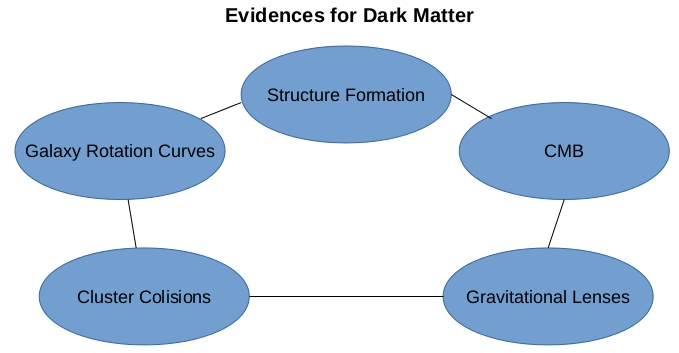
\includegraphics[scale=0.6]{evidences}
\label{fig:evidences}
\caption{Collections of the five most important evidences for Dark Matter. Hacer gáfica...}
\end{figure}

Decribe each one....

\section{Indirect Detection}



Dark matter particles that populate our universe in galactic and extragalactic scales may self-annihilate and produce a flux of gamma-rays, cosmic-rays, neutrinos, anti-matter which can appear as an excess over the expected background. The flux originated from dark matter annihilation should be proportional to the number density squared of particles, i.e. $\rho_{\chi}^2/m_{\chi}^2$, to the annihilation cross section $\sigma v$, to the element of volume of the sky observed accounted by $\Omega$, and the number of particles of interest produced per annihilation ($dN/dE$). Hence, it can we written as,

\begin{equation}
\underbrace{\frac{d\Phi}{d\Omega dE}}_{Diff. Flux} = {\color{blue} \frac{ \underbrace{ \sigma v }_{Anni.\, Cross\, Section}}{8\pi m_{\chi}^2}} \times {\color{green} \underbrace{\frac{dN}{dE}}_{Energy\, Spectrum}} \times {\color{red} \int_{l.o.s} ds} {\color{red}  \underbrace{\rho^2 (\overrightarrow{r}(s,\Omega))}_{Dark\, Matter\, Distribution}},
\label{eq:flux}
\end{equation}where $\Omega$ is truly the solid angle of the region of interest, $dN/dE$ is the energy spectrum (e.g. the number of photons produced per annihilation in case of gamma-rays), and $\rho (\overrightarrow{r}(s,\Omega))$ is the dark matter density which should integrated over the line of sight (l.o.s) from the observer to the source, which is often assumed to be described by either a Navarro-Frenk-White,
\begin{equation}
\rho(r) \propto \frac{r_s}{r[1+ r/r_s]^2},
\end{equation}or Einasto profile,
\begin{equation}
\rho(r) \propto exp \left[ \frac{-2.0}{\alpha} \left(\,  (r/r_s)^{\alpha}-1 \right) \right],
\end{equation}where $r_s=20$~kpc is the scale radius of the halo, and $\alpha=0.17$.



perfiles...

%\chapter{The Singlet-Doublet Fermion DM model (SDFDM)}
%%
\section{The model}
\label{sec:model}
The particle content of the model consists of two $SU(2)_L$-doublets of
Weyl fermions $\widetilde{R}_u$, $R_d$  with opposite hypercharges and one singlet
Weyl fermion $N$ of zero hypercharge. 
All of them are odd under one imposed $Z_2$ symmetry, under which the SM
particles are even. 
The new particle content is summarized in Table~\ref{tab:partcont}.
%
\begin{table}
  \centering
  \begin{tabular}{|l|l|l|l|}
    \hline  
    Symbol     & $\left( SU(2)_L, U(1)_Y \right)$ & $Z_2$ & \text{Spin}\\ \hline
    $N$  & $(1,0)$ & $-$ & 1/2\\
     $\widetilde{R}_u$, & $(2, +1/2)$ & $-$ & 1/2\\ 
     $R_d$ & $(2, -1/2)$ & $-$ & 1/2\\ \hline
  \end{tabular}
  \caption{$\alpha$-set of Weyl fermions of the model.}
  \label{tab:partcont}
\end{table}
%
The most general $Z_2$-invariant Lagrangian is given by
\begin{align}
\label{eq:lt13A}
 \mathcal{L}= &\mathcal{L}_{\text{SM}}+\mathcal{L}_{\text{Kin}}+ M_D \epsilon_{ab}R^a_d \widetilde{R}^b_u-\tfrac{1}{2}M_N NN-\lambda_d\, \epsilon_{ab}H^a R_d^b N-\lambda_u \epsilon_{ab}\widetilde{H}^a \widetilde{R}_u^b N+\text{h.c}
\end{align}
where $L_{i}$ are the lepton doublets,  we have defined the new $SU(2)_L$--doublets in terms of left-handed Weyl fermions as
\begin{align}
  R_{d}=&
  \begin{pmatrix}
    \psi_{L}^{0}\\
    \psi_{L}^{-}
  \end{pmatrix}
&  
\widetilde{R}_{u}=&
  \begin{pmatrix}
   - \left( \psi_{R}^{-} \right)^{\dagger}\\
     \left(\psi_{R}^{0}\right)^{\dagger}
  \end{pmatrix},
\end{align}
and $H$ is the SM Higgs doublet with $\widetilde{H}=i\sigma_2H^*$ and $v=246$ GeV.

Using the unitary gauge where  $H=\begin{pmatrix}0 & (h+v)/\sqrt{2}\end{pmatrix}^{\operatorname{T}}$ in the Eq.~\eqref{eq:lt13A} we have
\begin{align}
\label{eq:lt13a-expanded}
\mathcal{L}= &\mathcal{L}_{\text{SM}}+\mathcal{L}_{\text{Kin}}+ M_D(R_d^1\widetilde{R}_u^2-R_d^2\widetilde{R}_u^1)-\tfrac{1}{2}M_N NN
-\lambda_d(H^1R_d^2-H^2R_d^1)N-\lambda_u(\widetilde{H}^1R_u^2-\widetilde{H}^2R_u^1)N+\text{h.c}\nonumber \\
=&\mathcal{L}_{\text{SM}}+\mathcal{L}_{\text{Kin}}+ M_D(\psi_L^0{\psi_{R}^0 }^{\dagger}+\psi_L^-{\psi_{R}^- }^{\dagger})-\tfrac{1}{2}M_N NN
+\dfrac{\lambda_d (h+v)}{\sqrt{2}}\psi_L^0N - \dfrac{\lambda_u (h+v)}{\sqrt{2}}{\psi_R^0}^{\dagger}N +\text{h.c}\nonumber\\
=&\mathcal{L}_{\text{SM}}+\mathcal{L}_{\text{Kin}}+ \left[M_D\psi_L^0{\psi_{R}^0 }^{\dagger}-\tfrac{1}{2}M_N NN + \dfrac{\lambda_d v}{\sqrt{2}}\psi_L^0N - \dfrac{\lambda_u v}{\sqrt{2}}{\psi_R^0}^{\dagger}N\right]
+ M_D\psi_L^-{\psi_{R}^- }^{\dagger}
\nonumber\\ & 
+ \dfrac{h}{\sqrt{2}}\left(\lambda_d\psi_L^0N - \lambda_u{\psi_R^0}^{\dagger}N\right)+\text{h.c}.
%
\end{align}

The $Z_2$-odd fermion spectrum is composed by a
charged Dirac fermion $\chi^-=(\psi^-_L,\, \psi^-_R)^T$ with a tree
level mass $m_{\chi^\pm}=M_D$, and three Majorana fermions $\chi_i^0$ $(i=1,2,3)$ arisen from
the mixture between the neutral parts of the $SU(2)_L$ doublets and
the singlet fermion. 



%%%%%%%%%%%%%%%%%%%%%%%%%%%%%%%%%%%%%%%%%%%%%%%%%%%%%%%%%%%%%%%%%%%%%%%%%%%%%%%%%%%%%%%%%%%%%%%%%%%%%%
\subsection{Neutral mass spectra}
%
By defining the fermion basis through the vector:
\begin{align}
\label{eq:vecgauge}
\boldsymbol{\Xi}^{0}=
\begin{pmatrix}
N & R_d^1 & \widetilde{R}_u^2   
\end{pmatrix}^{\operatorname{T}}=
\begin{pmatrix}
N & \psi_L^0 & \psi_R^{0\dagger}
\end{pmatrix}^{\operatorname{T}},
\end{align} 
the neutral part of the Lagrangian can be writing like
\begin{align}
\label{eq:neutral_lagrangian}
\mathcal{L}_{\Xi}
=& \left[ M_D\psi_L^0{\psi_{R}^0 }^{\dagger}-\tfrac{1}{2}M_N NN
+\dfrac{\lambda_d v}{\sqrt{2}}\psi_L^0N 
- \dfrac{\lambda_u v}{\sqrt{2}} {\psi_R^0}^{\dagger}N\right] +\text{h.c}\nonumber\\
=&-\dfrac{1}{2}\bigg[M_N NN - M_D(\psi_L^0{\psi_{R}^0 }^{\dagger}+{\psi_{R}^0 }^{\dagger}\psi_L^0)
-\dfrac{\lambda_d v}{\sqrt{2}}(\psi_L^0N+N\psi_L^0) 
+\dfrac{\lambda_u v}{\sqrt{2}} ({\psi_R^0}^{\dagger}N+N{\psi_R^0}^{\dagger})\bigg] +\text{h.c}
\nonumber\\
  =&-\frac{1}{2}
\boldsymbol{\Xi}^{0\operatorname{T}}
\mathbf{M}^{\chi}\boldsymbol{\Xi}^0
+\text{h.c}\,,
\end{align}
where
\begin{align}
\label{eq:Mchi}
  \mathbf{M}^{\chi}=\begin{pmatrix}
  M_N                 &-\dfrac{\lambda_d v}{\sqrt{2}}&\dfrac{\lambda_u v}{\sqrt{2}}\\
-\dfrac{\lambda_d v}{\sqrt{2}} &  0                  & -M_D\\
\dfrac{\lambda_u v}{\sqrt{2}}&  -M_D                &  0  \\
\end{pmatrix}\,.
\end{align} 
If we define
%%%%%%%%%%%%%%%%%%%%%%%%%%%%%%%%%%%%%%%%%%%%%%%%%%%%%%%%
\begin{align}
  \label{eq:etabeta}
m_{\lambda}=&  \frac{\lambda v }{\sqrt{2}}\,,&
  \lambda=&\sqrt{\lambda_u^2+\lambda_d^2}\,,&
  \tan\beta=&\frac{\lambda_u}{\lambda_d}\, ,
\end{align}
the neutral fermion mass matrix will be given by
\begin{align}
\label{eq:Mchi}
  \mathbf{M}^{\chi}=\begin{pmatrix}
 M_N                 &-m_{\lambda}\cos\beta&m_{\lambda}\sin\beta\\
-m_{\lambda}\cos\beta &  0                  & -M_D\\
m_{\lambda}\sin\beta&  -M_D                &  0  \\
\end{pmatrix}\,,
\end{align}
which follow the same
convention of the bino-higgsino sector in the neutralino mass matrix of the
minimal supersymmetric standard model (MSSM)~\cite{Martin:2012us}. This convention facilitates the comparison between the present study and previous analysis
regarding the bino-higgsino DM limit of the MSSM. 
Such a limiting scenario occurs in the MSSM when the winos are decoupled from the spectrum and is accommodated within the SDFDM model when
$m_\lambda=m_Z\sin\theta_W$ ($\lambda=g'/\sqrt{2}$).




%%%%%%%%%%%%%%%%%%%%%%%%%%%%%%%%%%%%%%%%%%%%%%%%%%%%%%%%%%%%%%%%%%%%%%%%%%%%%%%%%%%%%%%%%%%%%%%%%
\subsection{Neutral mass eigenstates}
The Majorana fermion mass eigenstates $\mathbf{X}=(\chi_1^0,\chi_2^0,\chi_3^0)^T$ are obtained through the rotation
matrix $\mathbf{N}$\footnote{In~\cite{Horiuchi:2016tqw} we use $\mathbf{U}$ instead $\mathbf{N}$. The equivalence is $\mathbf{N}=\mathbf{U}^T$.} as 

%\begin{align}
%\mathbf{X}= \begin{pmatrix}\chi_1^0\\ \chi_2^0 \\ \chi_3^0\end{pmatrix}
%=\mathbf{U}  \begin{pmatrix}N\\ \psi_L^0 \\ (\psi_R^0)^\dagger\end{pmatrix}=\mathbf{U} \boldsymbol{\Xi}^0\,,
%\end{align}

\begin{align}
\label{eq:rotation}
\boldsymbol{\Xi}^0 = \begin{pmatrix}N\\ \psi_L^0 \\ (\psi_R^0)^\dagger\end{pmatrix}= 
\mathbf{N}\begin{pmatrix}\chi_1^0\\ \chi_2^0 \\ \chi_3^0\end{pmatrix}= \mathbf{N}\mathbf{X}
\end{align}
such that:

\begin{align}
\label{eq:chidiag}
 \mathbf{N}^{\operatorname{T}}\mathbf{M}^\chi \mathbf{N}=\mathbf{M}^\chi_\text{diag}\,,
\end{align}
%The usual suppersymmetric convention is E=N'^{\dagger}X -> N'^{*}M^{\chi}N'^{\dagger}=M^{\chi}_{diag}.
with
$\textbf{M}^\chi_{\text{diag}}=\operatorname{Diag}(m^\chi_1,m^\chi_2,m^\chi_3)$ and $m^\chi_n$ being the corresponding masses (no mass ordering is implied). 
In which follows we assume CP invariance and therefore $\mathbf{N}$ can be chosen real. Therefore, using the neutral Lagrangian Eq.~\eqref{eq:neutral_lagrangian} and the rotation Eq.~\eqref{eq:rotation}  we know that masses will be given by:

\begin{align}
\label{eq:masses_diag}
m^\chi_1=&\tfrac{1}{2}M_NN_{11}^2 - M_D N_{21}N_{31}-\dfrac{\lambda_dv}{\sqrt{2}}N_{11}N_{21}+\dfrac{\lambda_uv}{\sqrt{2}}N_{11}N_{31},\\
m^\chi_2=&\tfrac{1}{2}M_NN_{12}^2 - M_D N_{22}N_{32}-\dfrac{\lambda_dv}{\sqrt{2}}N_{12}N_{22}+\dfrac{\lambda_uv}{\sqrt{2}}N_{12}N_{32},\\
m^\chi_3=&\tfrac{1}{2}M_NN_{13}^2 - M_D N_{23}N_{33}-\dfrac{\lambda_dv}{\sqrt{2}}N_{13}N_{23}+\dfrac{\lambda_uv}{\sqrt{2}}N_{13}N_{33}\,.
\end{align}
%
The analytical diagonalization of the neutral fermion mass matrix is
carried out in Appendix~\ref{sec:analyt-form-mass} 
and for some analysis is convenient to have some approximate expressions in
the limit of small doublet-fermion mixing ($m_\lambda\ll M_D,M_N)$.
Expanding the analytical expressions for the eigensystem of
Eq.~\eqref{eq:chidiag} given in Appendix~\ref{sec:analyt-form-mass}
up to order $m_{\lambda}^2$, the fermion masses are given by
\begin{align}
\label{eq:ml2}
m^\chi_1=&M_{N} + \frac{M_{D} \sin{\left (2 \beta \right )} + M_{N}}{M_{N}^{2}- M_{D}^{2} }\, m_{\lambda}^{2}+\mathcal{O}\left( m_{\lambda}^4 \right) \nonumber\\
m^\chi_2=&M_{D} + \frac{ \sin(2 \beta ) + 1}{2 \left( M_{D} -  M_{N} \right)}\,m_{\lambda}^{2}+\mathcal{O}\left( m_{\lambda}^4 \right) \nonumber\\
m^\chi_3=&- M_{D} + \frac{ \sin(2 \beta ) - 1}{2 \left( M_{D} + M_{N} \right) }\,m_{\lambda}^{2}+\mathcal{O}\left( m_{\lambda}^4 \right)\,.
\end{align}
Approximate expressions for the mixing matrix are also given in the Appendix~\ref{sec:analyt-form-mass}.







%%%%%%%%%%%%%%%%%%%%%%%%%%%%%%%%%%%%%%%%%%%%%%%%%%%%%%%%%%%%%%%%%%%%%%%%%%%%%%%%%%%%%%%%%%%%%%%%%%%%%%%%%%%
\subsection{The interaction's Lagrangian}
%
Using the Lagrangian Eq.~\eqref{eq:lt13a-expanded}, the interaction terms in this model are
%
\begin{align}
\label{eq:lint1}
\mathcal{L} \, \supset \, \mathcal{L}_{\text{Int}}=&\mathcal{L}_{\text{Kin}}
- \dfrac{h}{\sqrt{2}}\left(-\lambda_d\psi_L^0N + \lambda_u{\psi_R^0}^{\dagger}N\right)+\text{h.c}\nonumber\\
= & \dfrac{1}{2}\bar{N}i\slashed{\partial}N + \bar{R_d}i\slashed{D}R_d + \bar{\widetilde{R}_u}i\slashed{D}\widetilde{R}_u
- \dfrac{h}{\sqrt{2}}\left(-\lambda_d\psi_L^0N + \lambda_u{\psi_R^0}^{\dagger}N+\text{h.c}\right)\,,
\end{align}
%
where $\slashed{D}$ is the covariant derivative. 
In the  Appendix~\ref{sec:lag-interaction}
we construct the Majorana spinor $X_i^0$ and the Dirac spinor $X^{\pm}$  as
\begin{align}
X_i^0=\begin{pmatrix}
(\chi_{i}^0)_\alpha \\ (\chi_i^{0\dagger})^{\dot{\alpha}}
\end{pmatrix}
=\begin{pmatrix}
N_{ji}\,\boldsymbol{\Xi}^{0}_j \\
N_{ji}^{\dagger}\,\boldsymbol{{\Xi}^{\dagger}}^{0}_j
\end{pmatrix}
\hspace{1.5 cm}
X^{\pm}=\begin{pmatrix}
\chi^{\pm}_{\alpha} \\ {\chi^{\mp}}^{\dagger\dot{\alpha}}
\end{pmatrix}
=\begin{pmatrix}
\psi_L^{\pm} \\
{\psi_R^{\mp}}^{\dagger}
\end{pmatrix}\,,
\end{align}
%
and we show that the interaction's Lagrangian is given by
%
\begin{align}
\label{eq:lint4}
\mathcal{L}_{\text{Int}}= & 
-\dfrac{g}{\sqrt{2}}\left(\bar{X}^-\slashed{W}\left(N_{2i}P_L-N_{3i}P_R\right)X_i^0 + \text{h.c}\right)
+ \dfrac{g}{4\cos\theta}\bar{X}_i^0\slashed{Z}\left(N_{2i}N_{2j}-N_{3i}N_{3j}\right)\gamma^5X_j^0 \nonumber\\
+& g\left(\dfrac{2\cos^2\theta_W-1}{2\cos\theta_W}\right)
\bar{X}^-\slashed{Z}X^-
-e\bar{X}^-\slashed{A}X^- 
-\dfrac{1}{\sqrt{2}}h\bar{X}_i^0\left(-\lambda_dN_{2i}N_{1j} + \lambda_uN_{3i}N_{1j}\right)X_j^0\,.
\end{align}
%
In particular, the interaction of the DM particle $X_i^0$ with the $W$, $Z$ and $h$ SM gauge boson is given by~\cite{Abdallah:2015ter}
%
\begin{align}
\mathcal{L^{\chi}}_{\text{Int}}=-\bar{X}^-\slashed{W}c_{WXX_i}X_i^0
-c_{ZX_iX_j}Z_{\mu}\bar{X}_i^0\gamma^{\mu}\gamma^{5}X_j^0
-c_{hX_iX_j}h\bar{X}_i^0X_j^0 \,,
\end{align}
where 
\begin{align}
c_{WXX_i}=& \dfrac{g}{\sqrt{2}}\left(N_{2i}P_L-N_{3i}P_R\right)  \label{eq:cWXXi}\\
c_{ZX_iX_j}=&\frac{g}{4\cos\theta_W}(N_{3i}N_{3j}-N_{2i}N_{2j}) \label{eq:cZXiXj}\\
%problema en el orden
c_{hX_iX_j}=&\frac{1}{\sqrt{2}}(-\lambda_dN_{2i}N_{1j}+\lambda_uN_{3i}N_{1j})\label{eq:cHXiXj}\,.
\end{align}
 
As is usually done, we denote the lightest stable particle in our model by $\chi^0$, whose couplings with the $Z$ and $h$ gauge bosons can explicitly written as~\cite{Calibbi:2015nha}
\begin{align}
c_{Z\chi^0\chi^0}&=-\frac{m_Z\lambda^2v(m_{\chi^0}^{2}-M_D^2)\cos2\beta}{2(m_{\chi^0}^{2}-M_D^2)^2+\lambda^2v^2\left(2\sin2\beta m_{\chi^0} M_D+m_{\chi^0}^{2}+M_D^2\right)},\label{eq:cZXX}\\
c_{h\chi^0\chi^0}&=-\frac{(M_D\sin 2\beta+m_{\chi^0})\lambda^2v}{M_D^2+\lambda^2v^2/2+2M_N\,m_{\chi^0}-3m_{\chi^0}^{2}}\label{eq:cHXX}.
\end{align}



%%%%%%%%%%%%%%%%%%%%%%%%%%%%%%%%%%%%%%%%%%%%%%%%%%%%%%%%%%%%%%%%%%%%%%%%%%%%%%
\section{Indirect detection}

%\subsection{DM self-annihilation channels}

\begin{figure}
\begin{center}
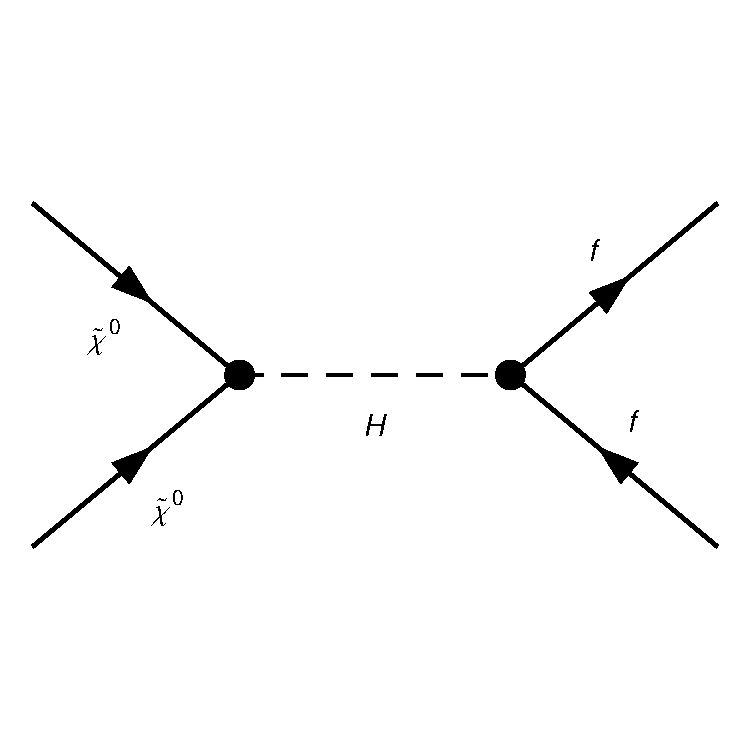
\includegraphics[scale=0.4]{XXHff}
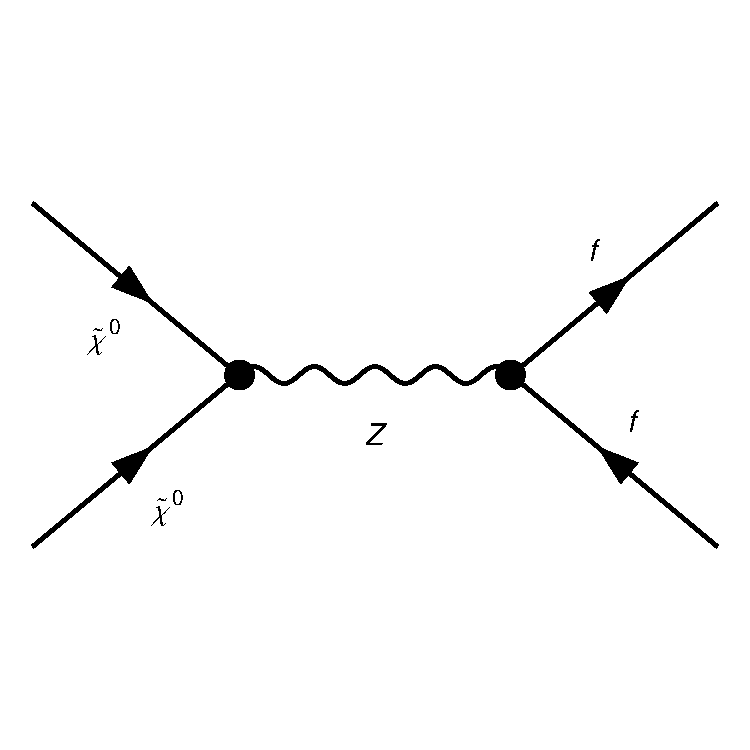
\includegraphics[scale=0.4]{XXZff}
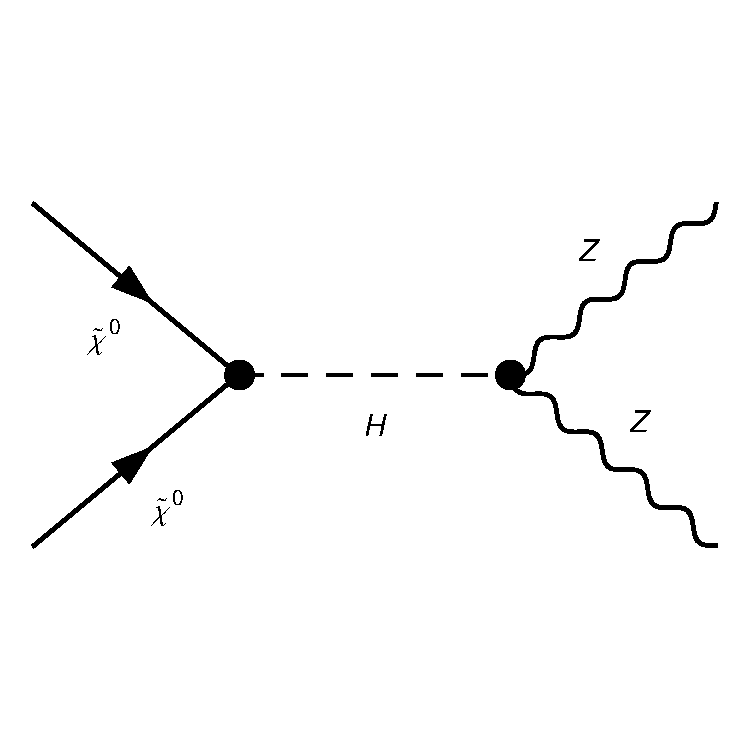
\includegraphics[scale=0.4]{XXHZZ}
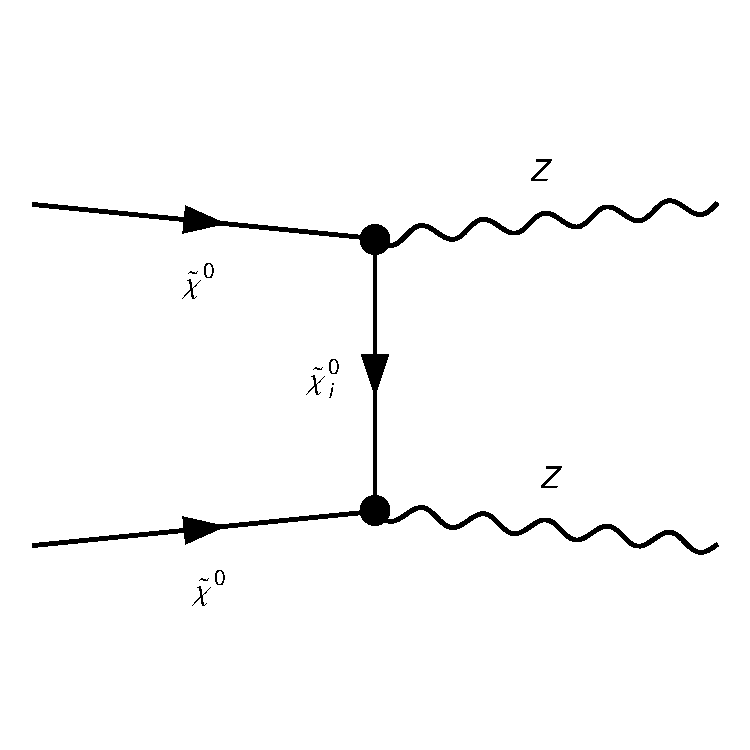
\includegraphics[scale=0.4]{XXXZZ}
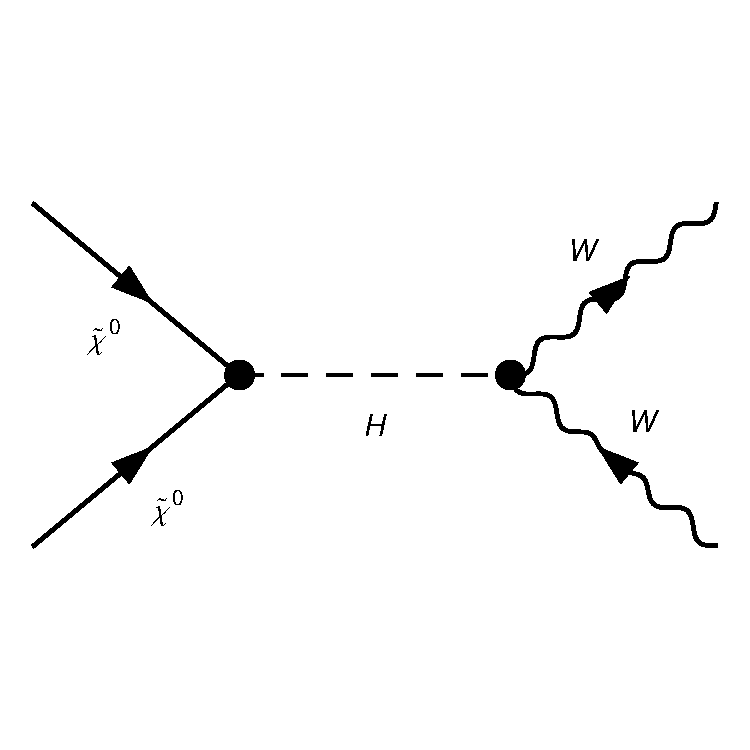
\includegraphics[scale=0.4]{XXHWW}
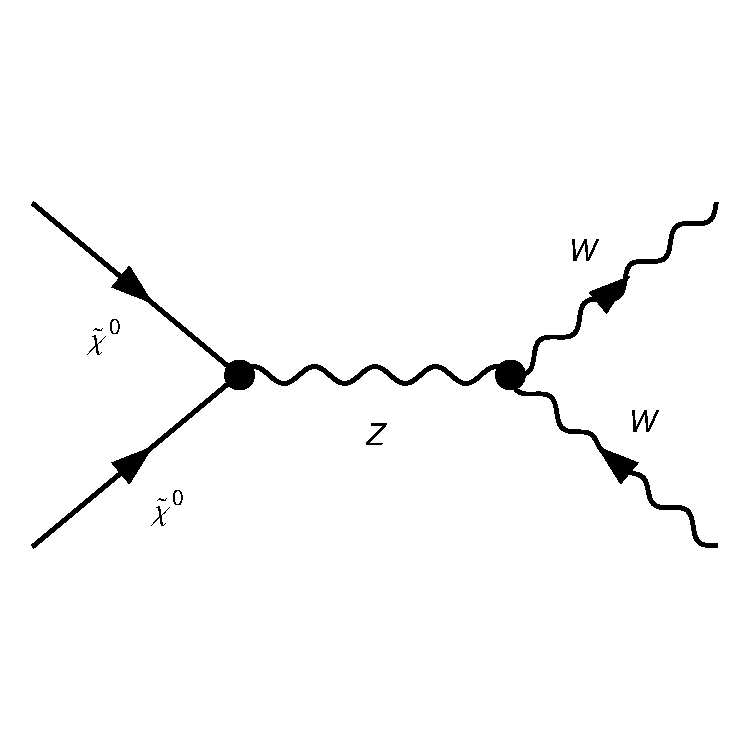
\includegraphics[scale=0.4]{XXZWW}
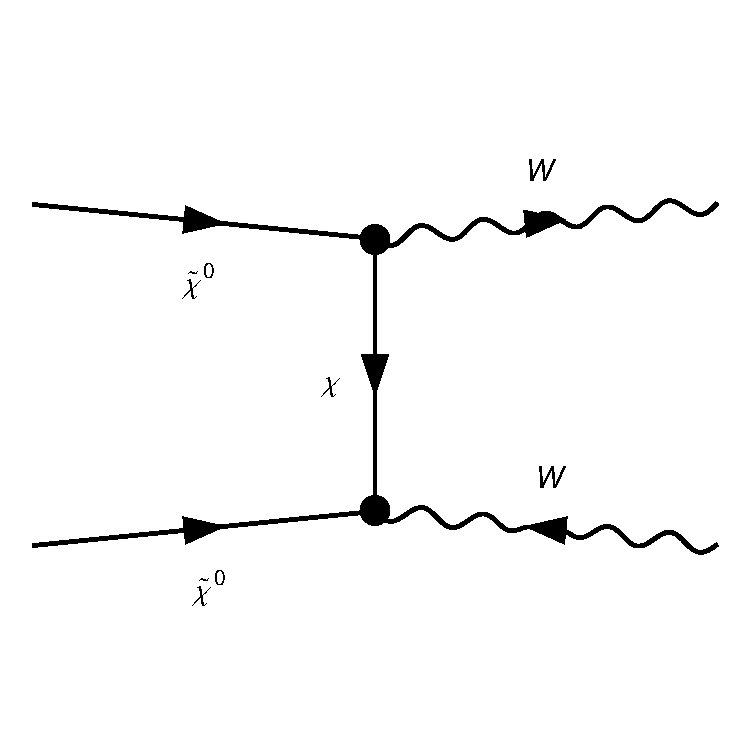
\includegraphics[scale=0.4]{XXXWW}
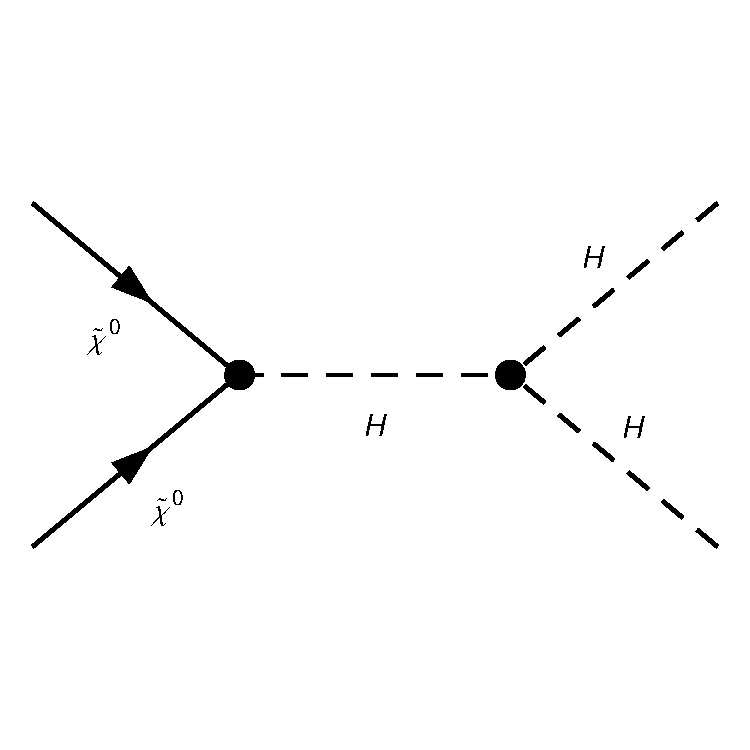
\includegraphics[scale=0.4]{XXHHH}
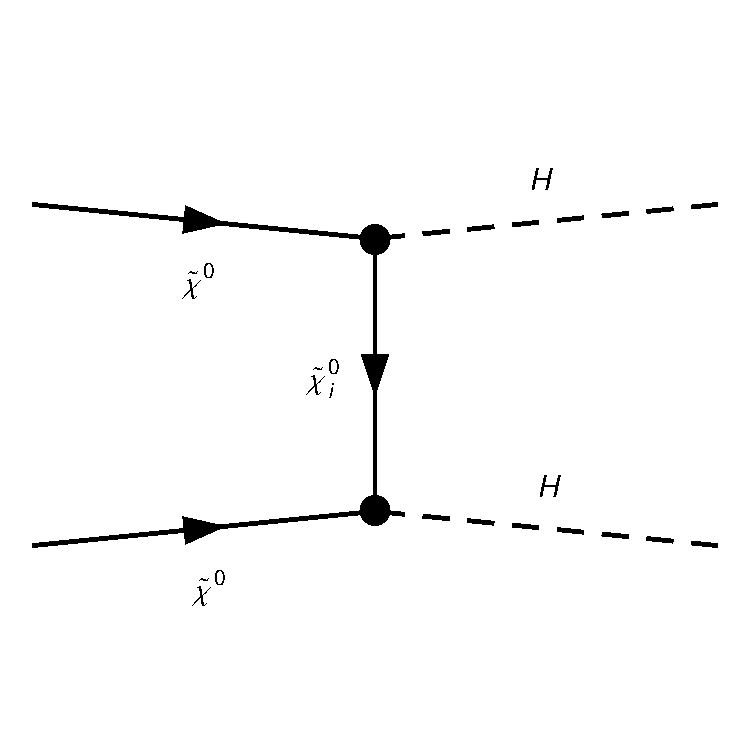
\includegraphics[scale=0.4]{XXXHH}
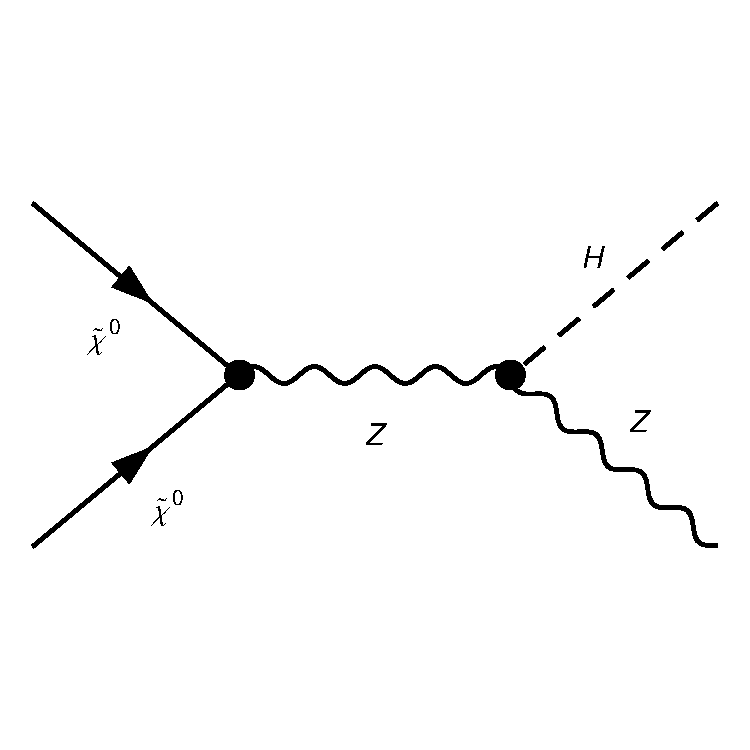
\includegraphics[scale=0.4]{XXZHZ}
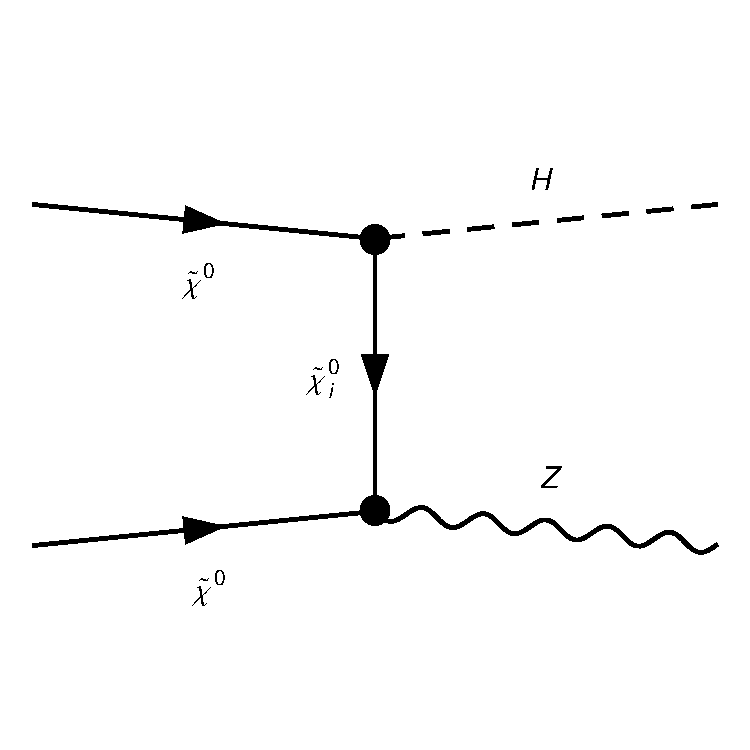
\includegraphics[scale=0.4]{XXXHZ}
\end{center}
\caption{Self-annihilation channels a tree level in the SDFDM model. The u-channels are not shown. They were generated using our implementation in \textsc{FeynArts}~\cite{Hahn:2000kx}.}
\label{fig:self-channels}
\end{figure}

At tree level, the interaction between the DM and the SM sector is mediated by the $W$, $Z$ and $H$ gauge bosons.
In this model, DM particles ($\chi^0$) can self-annihilate into $\bar{f}f$, $ZZ$, $W^+W^-$ and $hh$ final states through  $s$-channel Higgs and $Z$ boson exchange and into $ZZ$, $W^+W^-$ states via $t$-channel $\chi_i^0$ and $\chi^{\pm}$ exchange. Annihilations into a mixture of weak gauge bosons $Zh$ are also possible through the exchange of a $\chi_i\neq\chi^0$  in the $t$-channel or a $Z$ in the $s$-channel. Those annihilations channels are shown in the Fig.~\ref{fig:self-channels}.  We remark in passing that gamma-ray lines $\gamma\gamma$ and $\gamma Z$ can also be produced at one-loop level and it will be extensively discussed in the sec.~\ref{sec:gammarays-SDFDM}. 

Of particular importance for indirect detection studies in this framework is the fact that since DM annihilations into fermion pairs mediated by the Higgs are $p$-wave suppressed (there is no $s$-wave amplitude), the annihilations produced through $Z$ exchange are dominant. We note that the later is also helicity suppressed, this implies that the main annihilation channel is the $t\bar{t}$ ($b\bar{b}$) for a dark matter mass above (below) the top mass, with $\langle\sigma v \rangle\lesssim 10^{-27}$ cm$^3$ s$^{-1}$ for $m_{\chi^0}<m_W$ \cite{Calibbi:2015nha}. 

In the case scenario of DM particles going into gauge bosons, we find that only those processes in the $t$-channel are relevant because they do not suffer velocity suppression. Such a non-velocity suppression is also present in $s$ and $t$ channels for the annihilation into $Zh$. 
In contrast, we get that processes in which DM self-annihilates into a couple of Higgs bosons are velocity suppressed. 

%%%%%%%%%%%%%%%%%%%%%%%% PLOT SV %%%%%%%%%%%%%%%%%%%%%%%%%%%
\begin{figure}[h]
\begin{center}
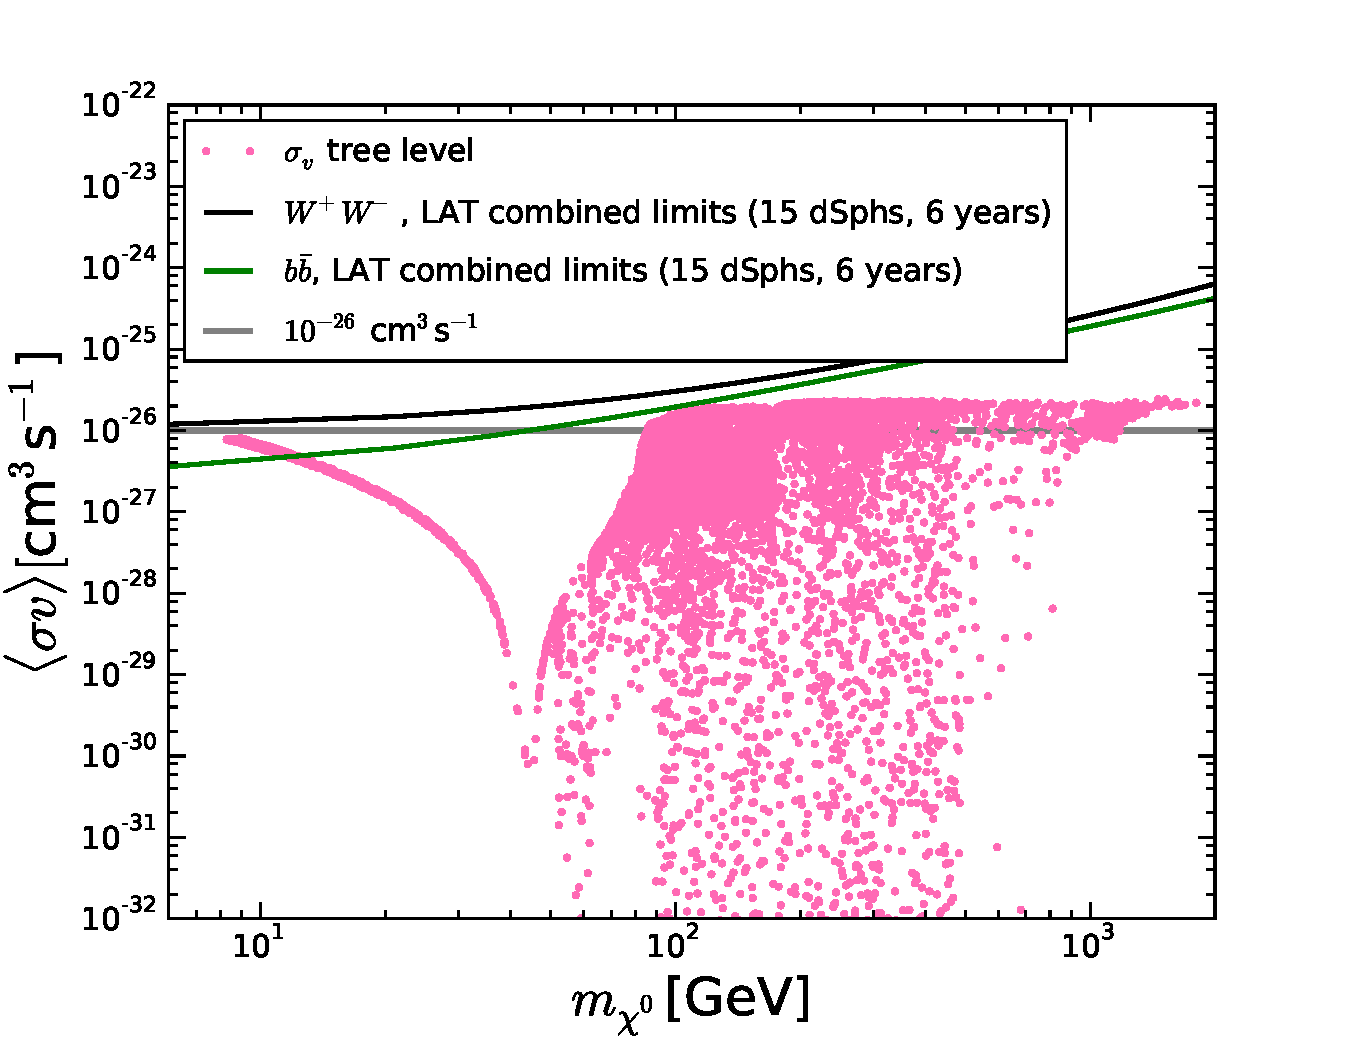
\includegraphics[scale=0.5]{sigmav-T13A}
\end{center}
\caption{Velocity average cross-section $\langle\sigma v\rangle$, generated randomly for a big sample of the parameters of the SDFDM model that take into account the correct relic density (see section~\ref{sec:Parameter-scan}). The green (black) line is the current constraint of indirect detection for DM annihilation into $b\bar{b}$ ($W^+W^-$) in the Dwarf spheroidal galaxies (dSph) at 95$\%$ C.L~\cite{Ackermann:2015zua}. The gray line represent the prediction of the WIMP paradigm where the $\langle\sigma v\rangle$ reach the thermal value $10^{-26}\text{cm}^{3}\text{s}^{-1}$.}
\label{fig:sigmav-random}
\end{figure}
%%%%%%%%%%%%%%%%%%%%%%%%%%%%%%%%%%%%%%%%%%%%%%%%%%%%%%%%%%%%%%%%%

In the Fig.~\ref{fig:sigmav-random} we show the total velocity average cross-section $\langle\sigma v\rangle$ for the self-annihilation of DM into SM particles including two and three final states compute with \textsc{micrOMEGAs 4.1.8}~\cite{Belanger:2014vza} through \textsc{Feynrules 2.3}~\cite{Christensen:2008py}. Each individual model (point) saturates the Planck measurement value for the relic density $\Omega h^2=(0.1199\pm0.0027)$~\cite{Ade:2013zuv} at $3\sigma$ level because we are interested in considering the case where this model accounts for the majority of the DM. It was generate randomly for a big sample of the parameters of the SDFDM model that we will describe latter in the section \ref{sec:Parameter-scan}. Also, we show the current and strogest \textit{Fermi}  Large Area Telescope (LAT) \footnote{\textit{Fermi}  Large Area Telescope: \url{http://fermi.gsfc.nasa.gov/}.} constraints of DM self-annihilation into $b\bar{b}$ quarks and $W^+W^-$ gauge bosons in the Dwarf spheroidal galaxies (dSph)~\cite{Ackermann:2015zua}. We see that indirect detection doesn't put strong constrains for the parameter space of the SDFDM model. All the models are alive with the current indirect detection constrains.    



%%%%%%%%%%%%%%%%%%%%%%%%%%%%%%%%%%%%%%%%%%%%%%%%%%%%%%%%%%%%%%%%%%%%%
\section{Direct detection}
Regarding direct detection, the Higgs $h$ ($Z$ gauge bosson) exchange leads to spin independent (spin dependent) DM nucleon scattering (see Fig.~\ref{fig:SD_SI}). From Eq.~\eqref{eq:cZXX} we get that the spin dependent (SD) cross section vanishes for $\cos2\beta=0$ or $|m_{\chi^0}|=M_D$, implying for both cases that $\tan\beta=\pm1$. In the same vein, from Eq.~\eqref{eq:cHXX} the spin independent (SI) cross section vanishes (i.e. a blind spot as discussed by Ref.~\cite{Cheung:2013dua}) for $\sin2\beta=-m_{\chi^0}/M_D$, which leads to $m_{\chi^0}=M_N, M_D$ using the characteristic equation of the Appendix~\eqref{sec:analyt-form-mass}. Note that $\sigma_{SI}=0$ if $\tan\beta<0$ and that only if $M_N>M_D$ both $\sigma_{SI}$ and $\sigma_{SD}$ can be zero simultaneously. 
%
\begin{figure}[h]
  \centering
  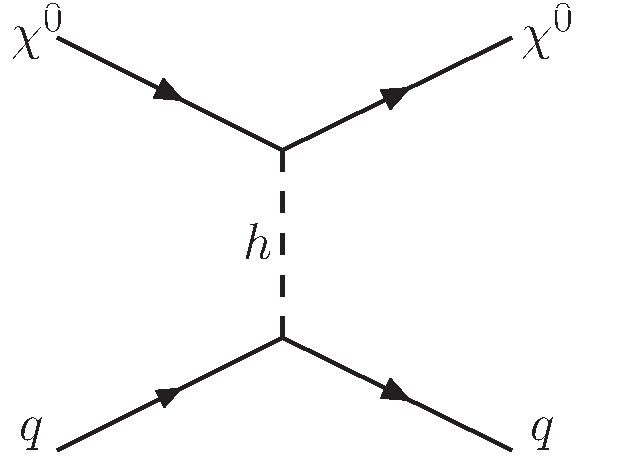
\includegraphics[scale=0.5]{SI} 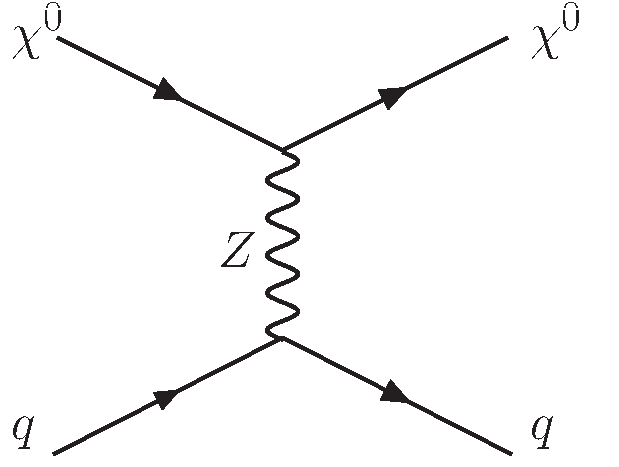
\includegraphics[scale=0.5]{SD}
  \caption{DM inelastic scattering with the quarks that compose the nucleons (protons and neutrons).}
  \label{fig:SD_SI}
\end{figure}





%%%%%%%%%%%%%%%%%%%%%%%%%%%%%%%%%%%%%%%%%%%%%%%%%%%%%%%%%%%%%%%%%%%%%%%%%%%%%%%%%%%%%%%%%%%%%%%%%%%%
\subsection{The spin independent cross section $\sigma_{SI}$}

The last scattering of the DM with the nucleons $N$ (protons and neutrons) is an effective interaction because nucleons are made of quarks. When the mediator is the Higgs gauge boson ($h$), we have an scalar interaction spin independent. In order to compute this scattering is reasonable to think in the next $h$ effective interaction with nucleons  
\begin{align}
\mathcal{L}_{\text{SM}}\supset & \sum_{q}\dfrac{m_q}{v}h\bar{q}q
= |N\rangle\langle N|\sum_{q}\dfrac{m_q}{v}h\bar{q}q |N\rangle\langle N|
= \dfrac{h}{v}\langle N|\sum_{q}m_q\bar{q}q|N\rangle |N\rangle\langle N|
=\dfrac{m_Nf_N}{v}h\bar{N}N\,,
\end{align}
where $\langle N|\sum_{q}m_q\bar{q}q|N\rangle=m_Nf_N$ is a QCD form factor~\cite{Belanger:2014vza},~\cite{Abdallah:2015ter} which is experimentally determined. 

The spin independent cross section a tree level is compute in the Appendix~\ref{sec:SI-amplitude}. It is given by
\begin{align}
\label{eq:SI-tree-level}
\sigma_{SI}=\dfrac{m_r^2}{\pi}\left(\dfrac{c_{hX_1X_1}}{vm_h^2}\right)^2f_N^2m_N^2\,,
\end{align}
%
where $m_r=\dfrac{m_Nm_{\chi^0}}{(m_N+m_{\chi^0})}$
is the DM nucleon reduce mass ($m_N\approx 0.939 \text{GeV}$ for the neutron and $m_N\approx 0.938 \text{GeV}$ for the proton). 

%%%%%%%%%%%%%%%%%%%%%%%%%%%%%%%%%%%% PLOT: SI %%%%%%%%
\begin{figure}[h]
\begin{center}
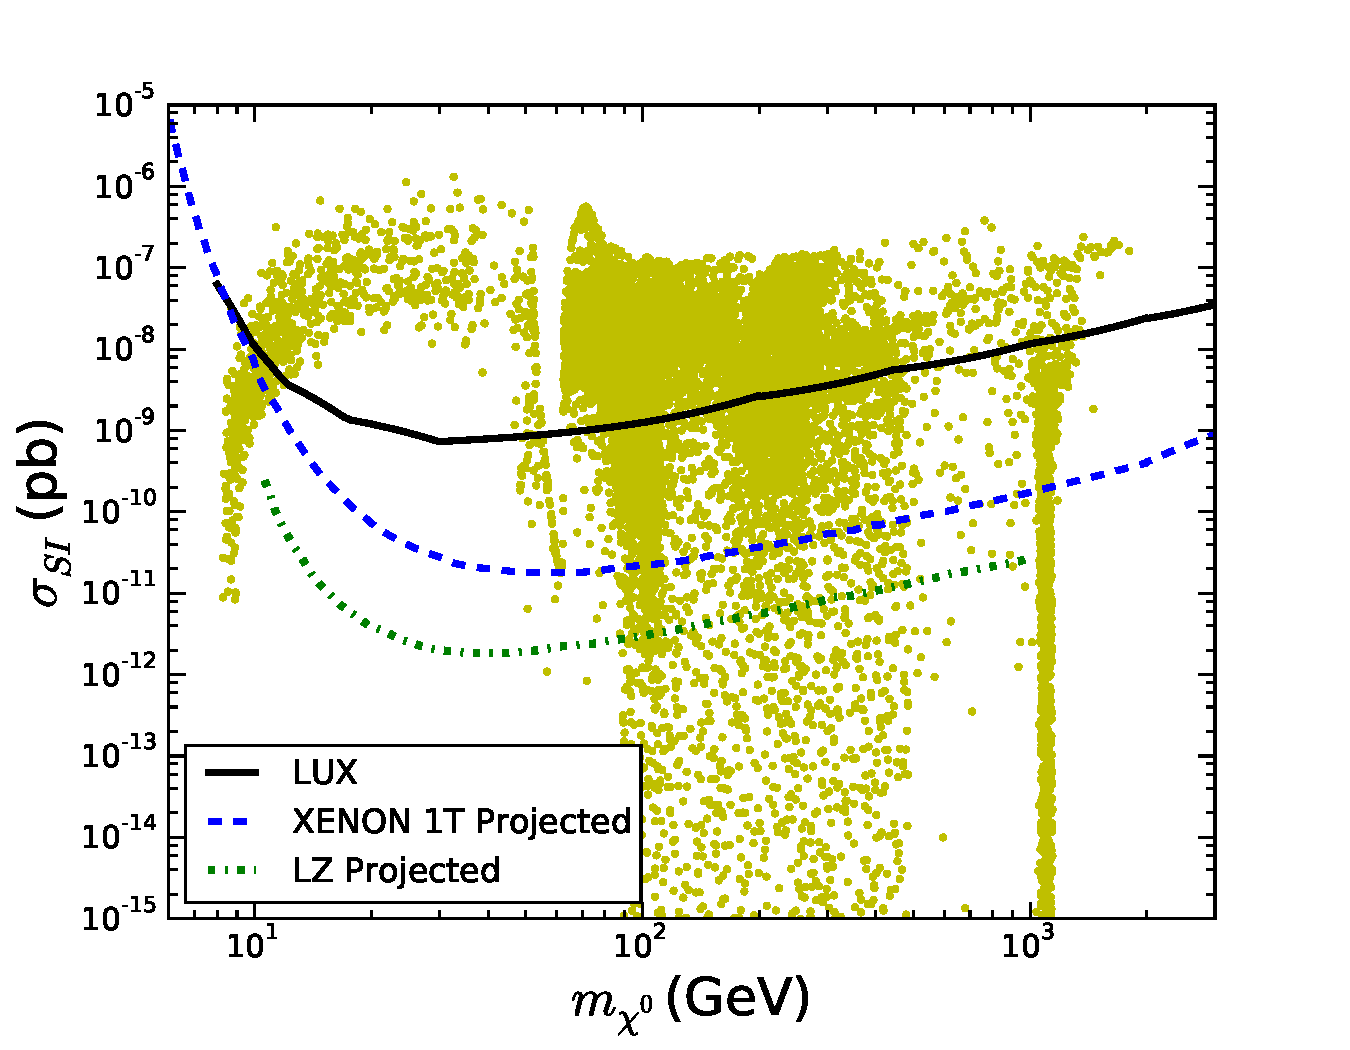
\includegraphics[scale=0.5]{sigmaSI-T13A}  
\caption{Spin-independent $\sigma_{SI}$  direct detection cross sections in the SDFDM model in comparison to current and future direct detection limits. 
The panel displays current limits from the LUX experiment (black solid line)~\cite{2013arXiv1310.8214L} and the expected limits from the forthcoming XENON-1T and LZ~\cite{Cushman:2013zza} experiments (blue dashed and green dot-dashed lines).
}
\label{fig:sigma-SI}
\end{center}
\end{figure}
%%%%%%%%%%%%%%%%%%%%%%%%%%%%%%%%%%%%%%%%%%%%%%%%%%%%%%

In the Fig.~\ref{fig:sigma-SI} we show the spin-independent $\sigma_{SI}$  direct detection cross sections compute with \textsc{micrOMEGAs 4.1.8}~\cite{Belanger:2014vza} through \textsc{Feynrules 2.3}~\cite{Christensen:2008py}. Each individual model (point) saturates the Planck measurement value for the relic density $\Omega h^2=(0.1199\pm0.0027)$~\cite{Ade:2013zuv} at $3\sigma$ level because we are interested in considering the case where this model accounts for the majority of the DM. It was generate randomly for a big sample of the parameters of the SDFDM model that we will describe latter in the section \ref{sec:Parameter-scan}. 
Also, we show the current limits from the LUX experiment (black solid line)~\cite{2013arXiv1310.8214L} and the expected limits from the forthcoming XENON-1T and LZ~\cite{Cushman:2013zza} experiments (blue dashed and green dot-dashed lines.  
We see that direct detection rule out some parameters space of this model. However some of the models are alive with the current direct detection constrains.     



%%%%%%%%%%%%%%%%%%%%%%%%%%%%%%%%%%%%%%%%%%%%%%%%%%%%%%%%%%%%%%%%%%%%%%%%%%%%%%%%%%%%%%%%%%%%%%%%%%%%%%%%%%%
\subsection{The spin dependent cross section $\sigma_{SD}$}

As we say before, when the mediator in the scattering of the DM with nucleons $N$ (protons and neutrons) 
is the $Z$ gauge boson, we have an interaction spin dependent.

%%%%%%%%%%%%%%%%%%%%%%%%%%%%%%%%%%%% PLOT: SD  %%%%%%%%%%%
\begin{figure}[h]
\begin{center}
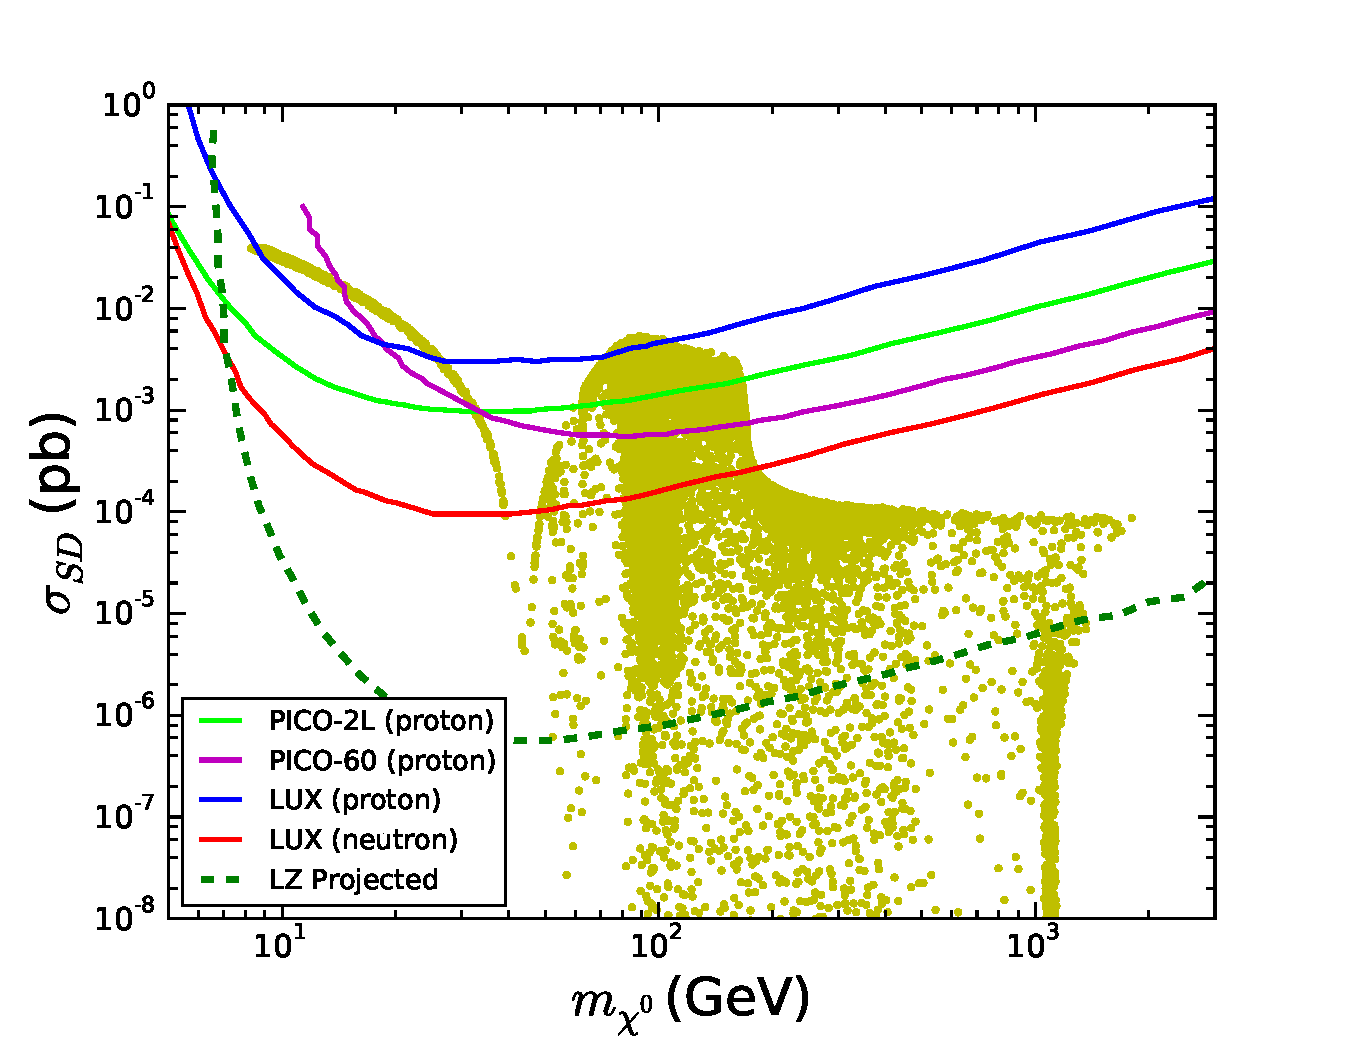
\includegraphics[scale=0.5]{sigmaSD-T13A} 
\caption{Spin-dependent $\sigma_{SD}$ direct detection cross sections in the SDFDM model in comparison to current and future direct detection limits. 
The panel shows the PICO-2L~\cite{Amole:2016pye} (green light solid line) and PICO-60~\cite{Amole:2015pla} (magenta solid line) limits as well as the LZ sensitivity (green dashed line). The most recent constraints from LUX~\cite{Akerib:2016lao} (red and blue solid lines) are also overlaid. 
}
\label{fig:sigma-SD}
\end{center}
\end{figure}
%%%%%%%%%%%%%%%%%%%%%%%%%%%%%%%%%%%%%%%%%%%%%%%%%%%%%%%%%%%%%%%

In the Fig.~\ref{fig:sigma-SD} we show the spin-dependent $\sigma_{SD}$  direct detection cross sections compute with \textsc{micrOMEGAs 4.1.8}~\cite{Belanger:2014vza} through \textsc{Feynrules 2.3}~\cite{Christensen:2008py}. Each individual model (point) saturates the Planck measurement value for the relic density $\Omega h^2=(0.1199\pm0.0027)$~\cite{Ade:2013zuv} at $3\sigma$ level because we are interested in considering the case where this model accounts for the majority of the DM. As we did for the $\sigma_{SI}$, it was compute randomly for a big sample of the parameters of the SDFDM model that we will describe latter in the section \ref{sec:Parameter-scan}. 
Also, we shows the PICO-2L~\cite{Amole:2016pye} (green light solid line) and PICO-60~\cite{Amole:2015pla} (magenta solid line) limits as well as the LZ sensitivity (green dashed line). The most recent constraints from LUX~\cite{Akerib:2016lao} (red and blue solid lines) are also overlaid. 
We see that direct detection rule out some parameters space of this model. However some of the models are alive with the current direct detection constrains, but in the future the LZ experiment will rule out or confirm this model.



%%%%%%%%%%%%%%%%%%%%%%%%%%%%%%%%%%%%%%%%%%%%%%%%%%%%%%%%%%%%%%%%%%%%%%%%%%%%%%%%%%%%%%%%%%%%%%%%%%%%%%%%%%%%
\section{Invisible decays}
In this model we have a new contribution to the Higgs and Z boson invisible decay fraction. Those are given by:

\begin{align}
\Gamma(h \rightarrow \chi\chi) = \dfrac{m_h}{4\pi}\bigg(1-\dfrac{4m_{\chi_1}^2}{m_h^2}\bigg)^{3/2}|c_{h\chi_1\chi_1}|^2
\end{align}
and
\begin{align}
\Gamma(Z \rightarrow \chi\chi) = \dfrac{m_Z}{6\pi}\bigg(1-\dfrac{4m_{\chi_1}^2}{m_Z^2}\bigg)^{3/2}|c_{Z\chi_1\chi_1}|^2 .
\end{align}

Therefore, in order to do a good an viable study in this model, we must to restrict the parameter space to all the points that have a BR($h\rightarrow\chi\chi) < 0.19$ to $2\sigma$ in accord with the LCH an ILC prospects~\cite{Bechtle:2014ewa} and $\Gamma(Z\rightarrow\chi\chi) \lesssim 3$ MeV in accord with LEP~\cite{ALEPH:2005ab}.





%%%%%%%%%%%%%%%%%%%%%%%%%%%%%%%%%%%%%%%%%%%%%%%%%%%%%%%%%%%%%%%%%%%%%%%%%%%%%%%%%%%%%%%%%%%%%%%%%%%%%%%%%%%
\section{STU parameters}
%
In this model, we have new contribution to the EW precision observables (EWPO). The oblique parameters $\Delta S$ and $\Delta T$ have new contributions. The strongest constraints come from $T$ parameters where $\Delta T$ scales as $\sim (\lambda_d^2-\lambda_u^2)^2$ ~\cite{Enberg:2007rp},~\cite{Calibbi:2015nha}. We see that this constraints is important for large $\lambda$ and large $\tan\beta$. We have took care of that.

%\chapter{The Singlet-Doublet Fermion DM model with real scalars singlets}
%\begin{flushright}
This chapter in based in our work publish in \textbf{PhysRevD.92.013005 (2015)}\\ 
\url{http://dx.doi.org/10.1103/PhysRevD.92.013005}
\end{flushright}
\begin{center}
\textbf{Abstrac}
\end{center}

  When the singlet-doublet fermion dark matter model is extended with
  additional $Z_2$--odd real  singlet scalars, neutrino masses and mixings
  can be generated at one-loop level.  In this work, we discuss the salient 
 features arising from the combination of the two resulting
  simplified dark matter models.  When the $Z_2$-lightest odd particle is a
  scalar singlet, $\operatorname{Br}(\mu\to e \gamma)$ could be
  measurable provided that the singlet-doublet fermion mixing is small
  enough. In this scenario, also the new decay channels of vector-like
  fermions into scalars can generate interesting leptonic plus
  missing transverse energy signals at the LHC. On the other hand, in
  the case of doublet-like fermion dark matter, scalar coannihilations
  lead to an increase in the relic density which allows to lower the bound of
  doublet-like fermion dark matter.

\section{Introduction to the neutrino masses in the SDFDM model}
%
In view of the lack of signals of new physics in strong production at the
LHC, there is a growing interest in simplified models where the
production of new particles is only through electroweak processes,
with lesser constraints from LHC limits.
In particular, there are simple standard model (SM) extensions with
dark matter (DM) candidates, such as the singlet scalar dark
matter (SSDM)
model~\cite{Silveira:1985rk,McDonald:1993ex,Burgess:2000yq}, or the
singlet-doublet fermion dark matter (SDFDM)
model~\cite{ArkaniHamed:2005yv,Mahbubani:2005pt,D'Eramo:2007ga,Enberg:2007rp,Cohen:2011ec,Cheung:2013dua}.
In this kind of models, the prospects for signals at LHC are in general
limited because of the softness of final SM particles coming from the
small charged to neutral mass gaps of the new particles, which is usually required 
to obtain the proper relic density.
In this sense, the addition of new particles, motivated for example by
neutrino physics, could open new detection possibilities, either
through new decay channels or additional mixings which increase the
mass gaps.

On those lines, scotogenic models~\cite{Ma:2006km}, featuring neutrino masses suppressed
by the same mechanism that stabilizes dark matter, have been thoroughly studied with specific predictions in almost all the
current terrestrial and satellite detector experiments (For a review
see for example~\cite{Boucenna:2014zba}).
The simplest models correspond to extensions of the inert doublet
model~\cite{Deshpande:1977rw,Barbieri:2006dq} with extra singlet or
triplet fermions.
Recently, the full list of 35 scotogenic models with neutrino masses at
one-loop~\cite{Ma:1998dn,Bonnet:2012kz}\footnote{The general
  realization of the Weinberg operator at two-loops have been undertaken
  in~\cite{Sierra:2014rxa}}, and at most triplet representations of
$SU(2)_L$, was presented in~\cite{Restrepo:2013aga} (and partially
in~\cite{Law:2013saa}).
The next to simplest scotogenic model is possibly the one where the
role of the singlet fermions is played by singlet scalars, and the role
of the scalar inert doublet is played by a vector-like doublet fermion.
One additional singlet fermion is required to generate neutrino masses
at one-loop level.
This kind of extension of the singlet dark matter model is labeled
as the model T13A with $\alpha=0$ in \cite{Restrepo:2013aga}. The
extra fermion, required in order to have radiative neutrino masses, can
be the singlet in the SDFDM model.

In the simplest scotogenic model~\cite{Ma:2006km}, singlet fermion
dark matter is possible but quite restricted by lepton flavor
violation (LFV)~\cite{Toma:2013zsa,Vicente:2014wga}. 
In contrast, we will show that in the present model the region of the
parameter space, corresponding to fermion dark matter, is well below
the present and near future constraints on $\operatorname{Br}(\mu\to
e\gamma)$.

On the other hand, when the lightest $Z_2$-odd particle (LOP) is one
of the scalar singlets, in the regions of the parameter space 
compatible with constraints from LFV, we could have promising signals at colliders,
thanks to the electroweak production of fermion doublets and possible
large branchings into charged leptons.

The dark matter phenomenology of both the SSDM and SDFDM models has
been extensively studied in the literature and recently
revisited in~\cite{Abe:2014gua}.
Here, we consider the possible effect of coannihilations with the
scalar singlets for fermion dark matter. 
We will see that these coannihilations tend to increase the relic
density of dark matter and may modify the viable parameter space of
the model. 
Specifically, they allow to reduce the lower bound on the mass of the
doublet-like dark matter particle from around $\SI{1100}{GeV}$ down to
about $\SI{900}{GeV}$.


%%%%%%%%%%%%%%%%%%%%%%%%%%%%%%%%%%%%%%%%%%%%%%%%%%%%%%%%%%%%%%%%%%%%%%%%%%%%%%%%%%%%%%%%%%%%%%%%%%%%%
\section{The model}
\label{sec:model-with-scalars}
This is an extension o the SDFDM model with a set of 
real scalar singlets  $S_{\alpha}$ of zero hypercharge
and odd under the imposed $Z_2$ symmetry. 
The new particle content is summarized in Table~\ref{tab:partcont}.
%
\begin{table}
  \centering
  \begin{tabular}{|l|l|l|l|}
    \hline  
    Symbol     & $\left( SU(2)_L, U(1)_Y \right)$ & $Z_2$ & \text{Spin}\\ \hline
    $S_{\alpha}$ & $(1,0)$ & $-$ & 0\\
    $N$  & $(1,0)$ & $-$ & 1/2\\
     $\widetilde{R}_u$, & $(2, +1/2)$ & $-$ & 1/2\\ 
     $R_d$ & $(2, -1/2)$ & $-$ & 1/2\\ \hline
  \end{tabular}
  \caption{$\alpha$-set of scalars and Weyl fermions of the model.}
  \label{tab:partcont}
\end{table}
%
Now with this extension, the most general $Z_2$-invariant Lagrangian is given by
\begin{align}
\label{eq:lt13a}
 \mathcal{L}= &\mathcal{L}_{\text{SM}}+ M_D \epsilon_{ab}R^a_d \widetilde{R}^b_u-\tfrac{1}{2}M_N NN-h_{i\alpha} \epsilon_{ab}\widetilde{R}_u^a L_{i}^b S_{\alpha}-\lambda_d\, \epsilon_{ab}H^a R_d^b N-\lambda_u \epsilon_{ab}\widetilde{H}^a \widetilde{R}_u^b N+\text{h.c}\nonumber\\
&-\left[ 
\tfrac{1}{2}\left({M}_S^2\right)_{\alpha\beta} S_{\alpha}S_\beta
   +\lambda^{SH}_{\alpha\beta} \epsilon_{ab}\widetilde{H}^{a}H^bS_{\alpha}S_{\beta}+\lambda^{S}_{\alpha\beta\gamma\delta}S_{\alpha}S_{\beta}S_{\gamma}S_{\delta} 
\right], 
\end{align}
where $L_{i}$ are the lepton doublets, $H$ is the SM Higgs, $N$ the new singlet fermion and $R_d$ and $\widetilde{R_u}$ the new $SU(2)_L$--doublets fermions of the SDFDM model.

In the scalar potential, we assume that the $M_{S}^{2}$ matrix has only
positive entries and $\left(M_S^2 \right)_{\alpha\beta}+\lambda^{SH}_{\alpha\beta}v^2=0$ for $\alpha\ne\beta$,  which means $S_\alpha$ are mass eigenstates with masses $m_{S_{\alpha}}^{2}=\left({M}_S^2 \right)_{\alpha\alpha}+\lambda^{SH}_{\alpha\alpha}v^2$ and $m_{S_\alpha}<m_{S_{\alpha+1}}$.
%

%In particular
%\begin{align*}
%  (\psi_R^{0})^\dagger=\mathbf{N}_{3m}\chi_m=[\mathbf{N}\mathbf{X}]_3\,.
%\end{align*}
%where $m=1,2,3$.
%
%
%The neutral Lagrangian  in the mass eigenstate basis includes
%\begin{align}
%\label{eq:masseig}
%  \mathcal{L}_0=&h_{i\alpha}\mathbf{N}_{3n}\chi_n \nu_{Li}S_\alpha+\frac{1}{2}\mathbf{X}^{\operatorname{T}}\mathbf{N}^T \mathbf{M}^{\chi}\mathbf{N}\mathbf{X}+\text{h.c}\nonumber\\
%=&h_{i\alpha}\mathbf{N}_{3n}\chi_n \nu_{Li}S_\alpha+\frac{1}{2}\chi_{m}\left( \mathbf{M}^{\chi}_{\text{diag}} \right)_{mn} \chi_{n} +\text{h.c}\nonumber\\
%=&h_{i\alpha}\mathbf{N}_{3n}\chi_n \nu_{Li}S_\alpha+\frac{1}{2}M_{\chi_n}\chi_n\chi_n +\text{h.c}\,.
%\end{align}

%%%%%%%%%%%%%%%%%%%%%%%%%%%%%%%%%%%%%%%%%%%%%%%%%%%%%%%%%%%%
\subsection{One-loop neutrino masses}

In this model, the new fields do not carry lepton number so that the
only lepton-number violating terms is the one with coupling $h_{i\alpha}$. The radiative neutrino mass matrix is obtained 
using the realization of the Weinberg operator a one-loop. In particular, we used the topology {\color{red}Tiii} described in the {\color{red}Appendix D}. 
The computation of the neutrino mass matrix can be done in the interaction basis as we show in the Appendix~\ref{sec:mass-interaction-basis}.
However, it is more illustrative if we do the computation in the basis of mass eigenstates. After the EWSB, each entry of the neutrino mass matrix have the three fermion contributions ($n=1,2,3$) displayed in Fig.~\ref{fig:T13Aweylme}, each one with a divergent parts which must cancel between them.  
\begin{figure}
  \centering
  %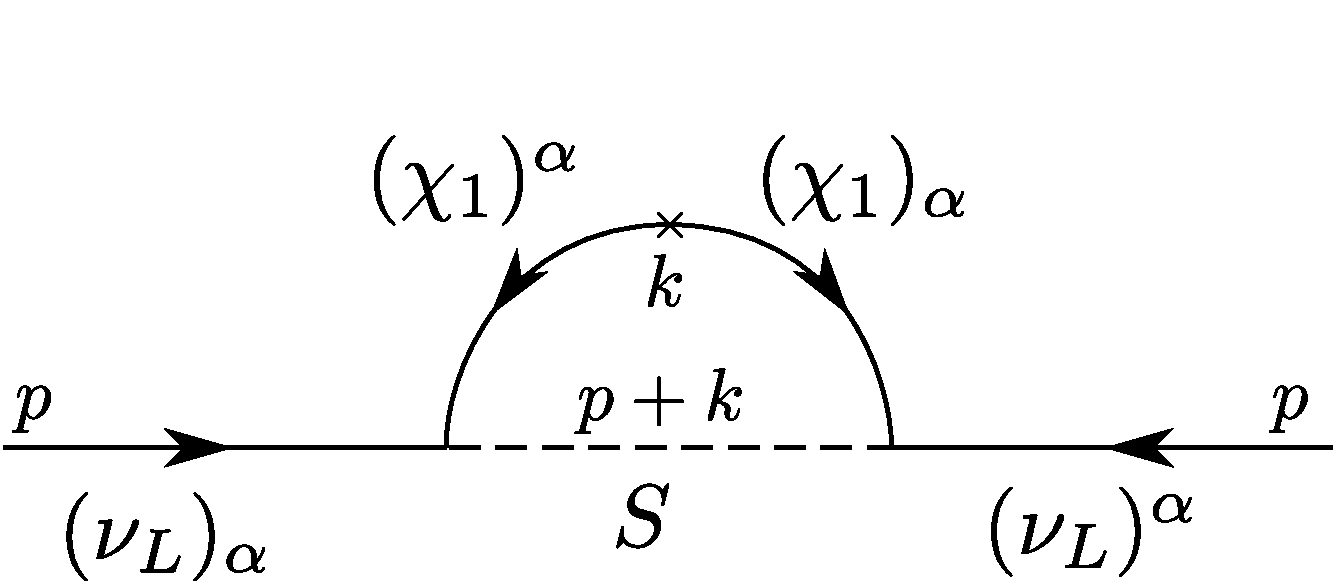
\includegraphics[scale=0.25]{T13Aweylme1} 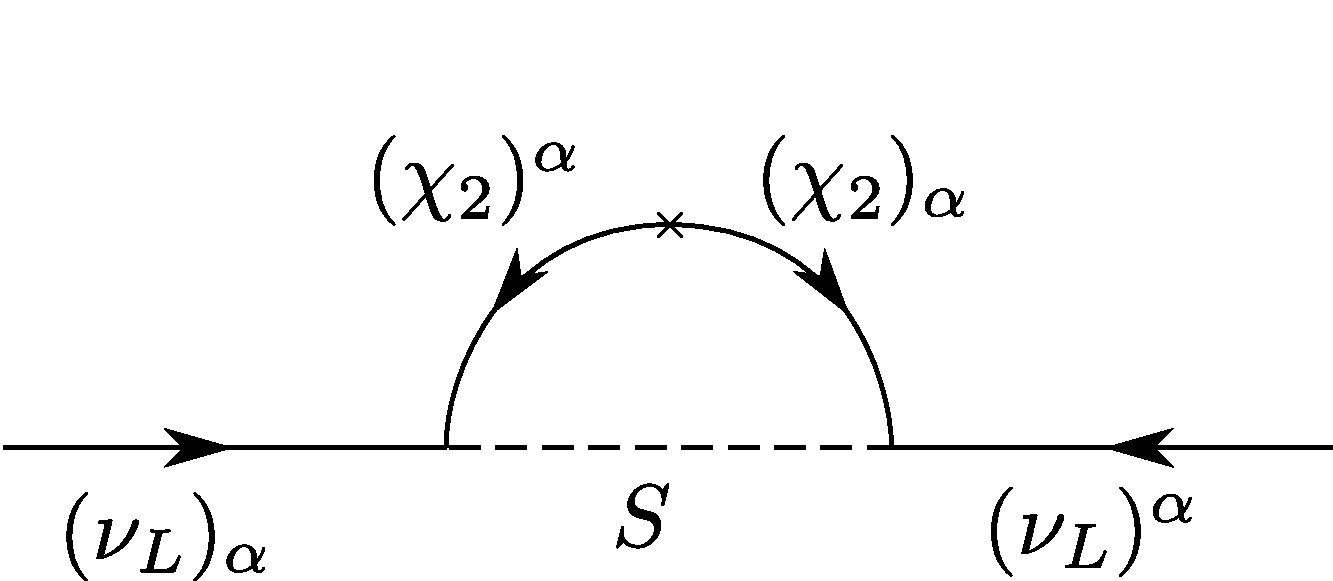
\includegraphics[scale=0.25]{T13Aweylme2} 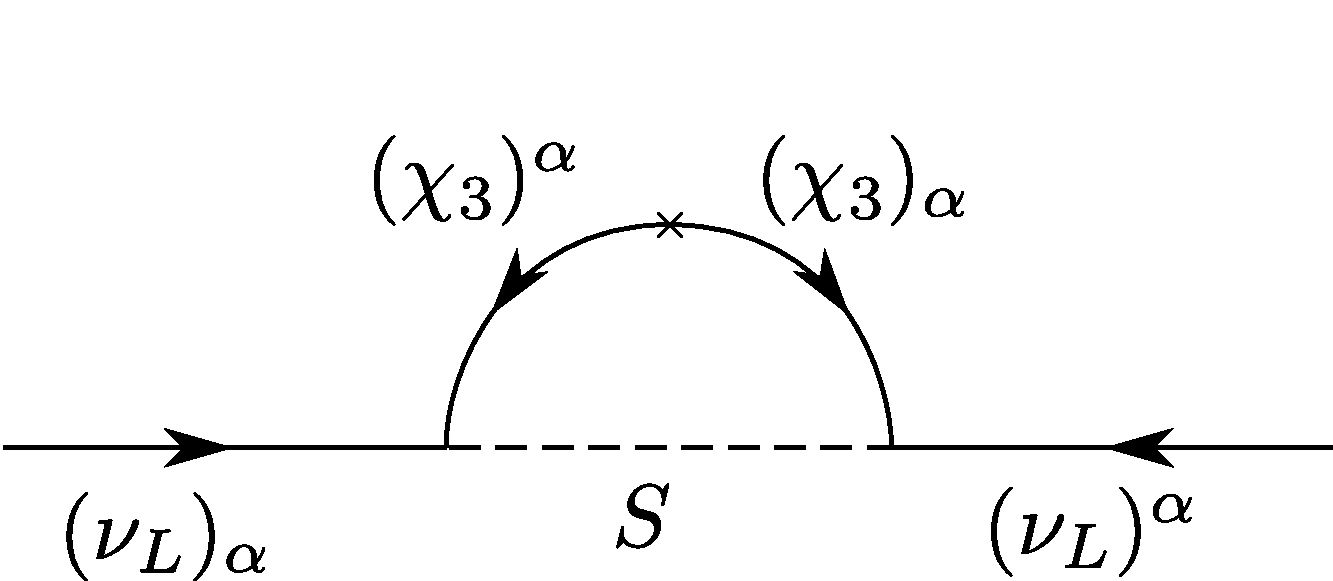
\includegraphics[scale=0.25]{T13Aweylme3}
  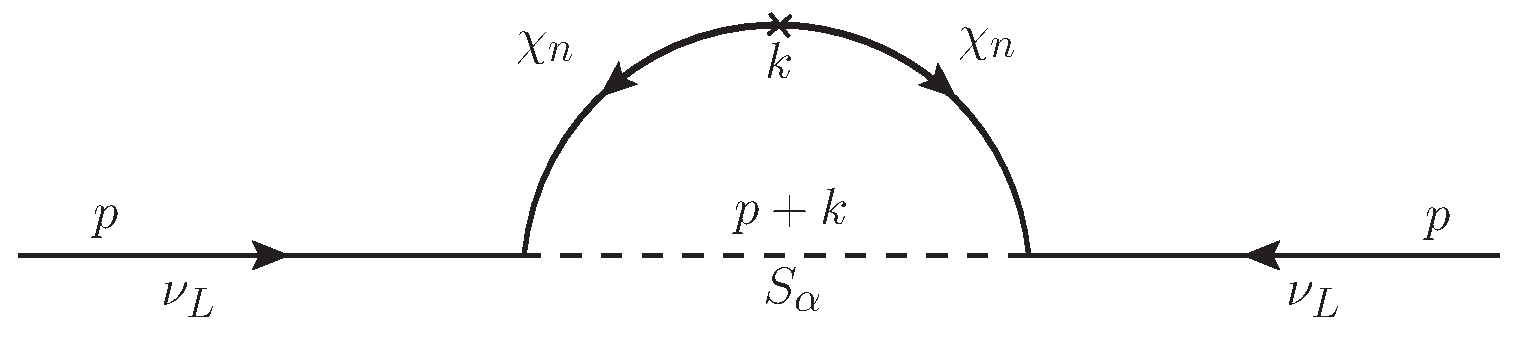
\includegraphics[scale=0.4]{neutrino_mass_diagram}
  \caption{Contributions to the neutrino mass matrix.}
  \label{fig:T13Aweylme}
\end{figure}

The neutrino mass matrix in this basis is given by
\begin{align*}
  M^{\nu}_{ij}=&i\sum_{\alpha}\int \frac{d^4k}{(2\pi)^4}\sum_{n=1}^3 \left( -i h_{i\alpha} N_{3n} \right) i S_F(k)\left( -i h_{j\alpha} N_{3n} \right)i\Delta_F(p+k)\nonumber\\
=&i\sum_{\alpha}\frac{h_{i\alpha}h_{j\alpha}}{16\pi^2}\sum_{n=1}^3 \left( N_{3n} \right)^2\int \frac{d^4k}{\pi^2}\frac{\cancel{k}+m_{\chi_n}}{\left(k^2-m_{\chi_n}^2  \right)\left[\left(p+k\right)^2-m_{S_\alpha}^2\right]}\,.
\end{align*}
In the limit $p\to 0$, we have
\begin{align}
\label{eq:mnueig}
  M^{\nu}_{ij}=&i^2\sum_{\alpha}\frac{h_{i\alpha}h_{j\alpha}}{16\pi^2}\sum_{n=1}^3 \left( N_{3n} \right)^2m_{\chi_n}\; B_0 \left(0;m_{\chi_n}^2,m^2_{S_{\alpha}} \right)\,,
\end{align}
where
\begin{align}
B_0 \left(0;m_{\chi_n}^2,m^2_{S_{\alpha}} \right)=&\int \frac{d^4k}{i\pi^2}\frac{1}{\left(k^2-m_{\chi_n}^2\right)\left(k^2-m_{S_\alpha}^2\right)}
=\frac{1}{m_{\chi_n}^2-m_{S_\alpha}^2}\left[ A_0\left(m_{\chi_n}^2\right)-A_0\left(m_{S_\alpha}^2\right)  \right],
\end{align}
with $A_0\left(m^2\right)=m^2 \left[ \Delta+1-\ln \left( m^2/\mu^2 \right) \right]$ and $ \Delta=\left( \frac{2}{\epsilon}-\ln\pi+\gamma_E \right)$, are Passarino Veltman functions~\cite{Passarino:1978jh}. 

In order to compute our matrix, we use two known things. 
First, if we use the Eq.~\eqref{eq:mnueig}, we have that the term
\begin{align}
\label{eq:mnueigdev}
\sum_{n=1}^3& \left( N_{3n} \right)^2m_{\chi_n}\; B_0 \left(0;m_{\chi_n}^2,m^2_{S_\alpha} \right)\nonumber\\
  &=\sum_{n=1}^3 \left( N_{3n} \right)^2m_{\chi_n}
   \left\{\frac{1}{m_{\chi_n}^2-m_{S_\alpha}^2}\left[m^2_{\chi_n} \left[ \Delta+1-\ln \left( m_{\chi_n}^2/\mu^2 \right) \right]   
-m_{S_\alpha}^2 \left[ \Delta+1-\ln \left( m_{S_\alpha}^2/\mu^2 \right) \right]\right] \right\}\nonumber\\
&=\sum_{n=1}^3 \left( N_{3n} \right)^2m_{\chi_n}
   \left\{(\Delta+1)+\frac{m_{S_\alpha}^2\ln \left( m_{S_\alpha}^2/\mu^2 \right)-m_{\chi_n}^2\ln \left( m_{\chi_n}^2/\mu^2 \right)}{m_{\chi_n}^2-m_{S_\alpha}^2} \right\}\nonumber\\
&=\sum_{n=1}^3 \left( N_{3n} \right)^2m_{\chi_n}
   \left\{\left[\Delta+1+\ln\left( \mu^2 \right) \right]+\frac{m_{S_\alpha}^2\ln \left( m_{S_\alpha}^2 \right)-m_{\chi_n}^2\ln \left( m_{\chi_n}^2 \right)}{m_{\chi_n}^2-m_{S_\alpha}^2} \right\}\,,
\end{align}
%
and second, y we use the Eq.~\eqref{eq:chidiag}, we obtain 
$\mathbf{N} \mathbf{M}^\chi_{\text{diag}}\mathbf{N}^{\operatorname{T}}=\mathbf{M}^\chi\Rightarrow \sum_mN_{lm}m_{\chi_m} N_{nm}=(M^\chi)_{ln}\,,$
and therefore,
\begin{align}
\label{eq:divcan}
  \sum_m N_{3m}^2m_{\chi_m}=(M^\chi)_{33}=0\,,
\end{align}
where we used the explicit expression for $\mathbf{M}^{\chi}$ given in the Eq.~\eqref{eq:Mchi} for $l=n=3\,$.
 
Therefore, using the Eq.~\eqref{eq:mnueigdev} and Eq.~\eqref{eq:divcan} we finally get that
\begin{align}
\label{eq:neutrino-mass-matrix}
M^{\nu}_{ij}=&\sum_{\alpha}\frac{h_{i\alpha}h_{j\alpha}}{16\pi^2}\sum_{n=1}^3 \left( N_{3n} \right)^2m_{\chi_n}
\left[ \frac{m_{\chi_n}^2\ln \left( m_{\chi_n}^2 \right)-m_{S_\alpha}^2\ln \left( m_{S_\alpha}^2 \right)}{m_{\chi_n}^2-m_{S_\alpha}^2} \right]\,.
\end{align}

%%%%%%%%%%%%%%%%%%%%%%%%%%%%%%%%%%%%%%
\subsection{Casas-Ibarra parametrization in the this model}
We can write the neutrino mass matrix~\eqref{eq:neutrino-mass-matrix} as 
%
\begin{align}
   M^{\nu}_{ij}=&\sum_{\alpha}\frac{h_{i\alpha}h_{j\alpha}}{16\pi^2}\sum_{n=1}^3 \left( N_{3n} \right)^2m_{\chi_n}
\,f\left( m_{S_\alpha},m_{\chi_n} \right) ,\\\label{eq:Mnuij}
=&\sum_{\alpha} h_{i\alpha} \Lambda_{\alpha} h_{j\alpha}\\\label{eq:CI}
=&\left( \mathbf{h}\mathbf{\Lambda}\mathbf{h}^{\operatorname{T}} \right)_{ij}\,,
\end{align}
with
$f \left( m_1,m_2 \right)= (m_1^2\,\ln  m_1^2 -m_2^2\,\ln m_2^2 )/(m_1^2-m_2^2)$, $\boldsymbol{\Lambda}=\operatorname{Diag}\left(\Lambda_1,\Lambda_2,\Lambda_3\right)$ and
\begin{align}
\label{eq:Lambda}
  \Lambda_\alpha=&\frac{1}{16\pi^2}\sum_{n=1}^3 \left( N_{3n} \right)^2m_{\chi_n}\,f\left( m_{S_\alpha},m_{\chi_n} \right).
\end{align}

As we described in the Appendix~\ref{sec:casas-ibarra}, the flavor structure of the neutrino mass matrix $M^{\nu}_{ij}$, given
by Eq.~\eqref{eq:CI}, allows us to express the Yukawa couplings in
terms of the neutrino oscillation observables (ensuring the proper
compatibility with them) through the Casas-Ibarra parametrization introduced in
\cite{Casas:2001sr,Ibarra:2003up}. 
Thus, by using an arbitrary complex orthogonal rotation matrix
$\boldsymbol{\mathcal{R}}$, the Yukawa couplings $h_{i\alpha}$ are
given by
\begin{align}
  \label{eq:ht}
  \mathbf{h}^{T}=\mathbf{D}_{\sqrt{{\Lambda}^{-1}}}\,\boldsymbol{\mathcal{R}}\,\mathbf{D}_{\sqrt{m_{\nu}}}\,\mathbf{U}^{\dagger} \,,
\end{align}
where $\mathbf{D}_{\sqrt{m_\nu}}=\operatorname{Diag}
\left(\sqrt{m_{\nu 1}} , \sqrt{m_{\nu2}},\sqrt{m_{\nu3}}\right)$,
$\mathbf{D}_{\sqrt{\Lambda^{-1}}}=\operatorname{Diag}
\left(\sqrt{\Lambda_1^{-1}} , \sqrt{\Lambda_2^{-1}},\cdots\right)$ and
$\mathbf{U}$ is the PMNS~\cite{Maki:1962mu} neutrino mixing matrix.

Henceforth
we will consider the case of three scalar singlets, $\alpha=1,2,3$,
where the Yukawa couplings take the form
\begin{align}
\label{eq:Y_CIww}
 h_{i\alpha}=&\frac{\sqrt{m_{\nu 1}}{\mathcal{R}}_{\alpha 1}U_{i1}^*+\sqrt{m_{\nu 2}}{\mathcal{R}}_{\alpha 2} U^{*}_{i2}+ \sqrt{m_{\nu 3}}{\mathcal{R}}_{\alpha 3} U^{*}_{i3}}{\sqrt{\Lambda_\alpha}}.
\end{align}
In the above equation, the $3\times3$ matrix
$\boldsymbol{\mathcal{R}}$ can be cast in terms of three rotation
angles $\theta_{23},\theta_{13},\theta_{12}$, which are assumed to be real. 
It is worth mentioning that for the case two scalar singlets
$\alpha=1,2$ a viable scenario is also possible with the remarks that
one massless neutrino is obtained. 
To fully exploit the generality of $h_{i\alpha}$ couplings obtained
from~\eqref{eq:Y_CIww}, we stick to the case with three scalar singlets.


In summary, the set of input parameters of the model are the scalar masses
$m_{S_\alpha}$, $M_N$, $M_D$, $\lambda$,
$\tan\beta$, the lightest neutrino mass $m_{\nu1}$, the three rotation 
angles present in $\boldsymbol{\mathcal{R}}$  
and $\lambda^{SH}_{\alpha\beta}$\footnote{The couplings $\lambda^{S}_{\alpha\beta\gamma\delta}$ are irrelevant for phenomenological purposes.}. Without not loss of generality we assume for the latter to be small $\lambda^{SH}_{\alpha\beta}\lesssim0.01$, except for the case of scalar dark matter where $\lambda^{SH}_{11}$ is set to give 
the proper relic density.

In order to have an approximate expression for $\Lambda_\alpha$ in terms of this set of input parameters, we can use the identity~(\ref{eq:divcan}) to obtain
\begin{align*}
\Lambda_\alpha=&\frac{1}{16\pi^2}\left\{N_{31}^2\,m^\chi_1\left[ f(m_{S_\alpha},m^\chi_1)-f(m_{S_\alpha},m^\chi_3)\right]
                                +N_{32}^2\,m^\chi_2\left[f(m_{S_\alpha},m^\chi_2)-f(m_{S_\alpha},m^\chi_3)\right]\right\}\,.
\end{align*}
The expression for the matrix elements $N_{31}^2$ at $\mathcal{O}\left( m_{\lambda}^2 \right)$ are given in the Appendix~\ref{sec:analyt-form-mass}. Since $N_{31}^2$ and $f(m_{S_\alpha},m^\chi_2)-f(m_{S_\alpha},m^\chi_3)$ are already $\mathcal{O}\left( m_{\lambda}^2 \right)$, we can use the leading order values for the other masses and mixings parameters to obtain
\begin{align*}
  \Lambda_\alpha\approx&\frac{1}{16\pi^2}\left\{N_{31}^2 M_N\left[ f(m_{S_\alpha},M_N)-f(m_{S_\alpha},M_D)\right]
                                +\frac{1}{2}M_D\left[f(m_{S_\alpha},m^\chi_2)-f(m_{S_\alpha},m^\chi_3)\right]\right\}
+\mathcal{O}\left( m_\lambda^4 \right)\,.
\end{align*}
With the last two approximate formula for masses in \eqref{eq:ml2},  and the $N_{31}^2$  mixing in~\eqref{eq:mixl2}, we have
\begin{align}
\label{eq:lambdaappr}
16\pi^2\frac{\Lambda_\alpha}{m_{\lambda}^{2}}\approx & \left(\frac{M_{D} \cos\beta + M_{N} \sin\beta}{M_{D}^{2} - M_{N}^{2}}\right)^{2}
                                  M_{N}\left[f(m_{S_\alpha},M_N)-f(m_{S_\alpha},M_D)\right]\nonumber\\
&+\frac{ M_{D}^{2}\left[M_{D} \sin\left(2 \beta \right ) + M_{N}\right] 
        }{\left(M_{D}^{2} - M_{N}^{2}\right) \left(M_{D}^{2} - m_{S_\alpha}^{2}\right)^{2}} \left\{M_{D}^{2} - m_{S_\alpha}^{2} \left[\log{\left (\frac{M_{D}^{2}}{m_{S_\alpha}^{2}} \right )} + 1\right]\right\}+\mathcal{O}\left( m_\lambda^2 \right)\,.
\end{align}
%
To illustrate the dependence in $\tan\beta$ of $\Lambda_{\alpha}$, we consider the following set of input masses (SIM) compatible with singlet scalar dark matter:
\begin{align}
\label{eq:bp}
  m_{S_1}&=\SI{60}{GeV} & m_{S_2}=&\SI{800}{GeV} & m_{S_3}=&\SI{1500}{GeV}\, \nonumber\\
  m_N&=\SI{100}{GeV} & m_D=&\SI{550}{GeV}\,.
\end{align}
The results for $\lambda=\num{5E-3}$ are shown in
Fig.~\ref{fig:Lambdaa}(a). For large values of $\tan\beta$, the
$\Lambda_{\alpha}$ are positive. However, there are specific values of $\tan\beta$ for which each $\Lambda_{\alpha}$ 
goes to zero and turns to negative values, as illustrated by the red lines in the plot. 
The specific point with $\beta=\pi/6$ is depicted by the yellow stars in the figure.

\begin{figure}
\centering
(a) \hfill (b)\\
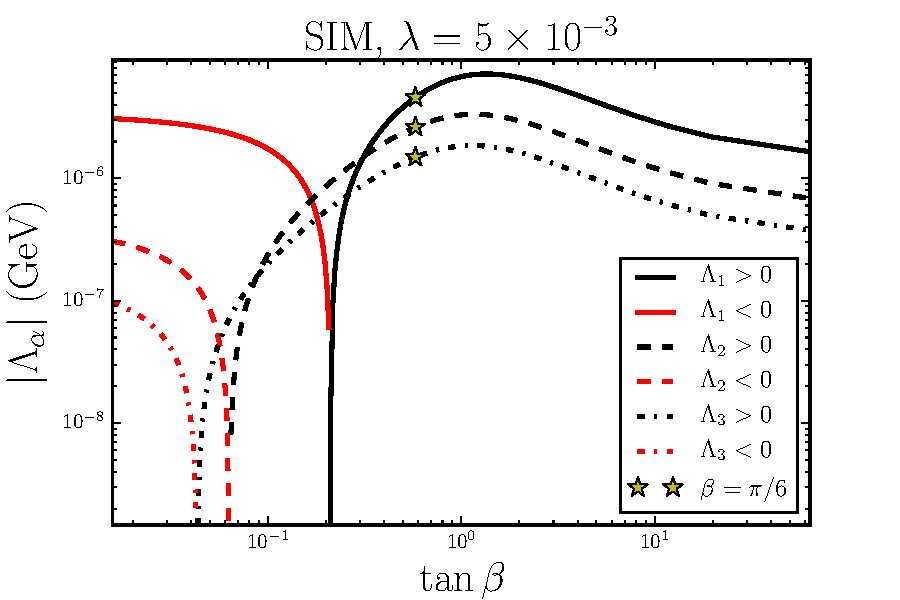
\includegraphics[scale=0.58]{tanbdependence}    
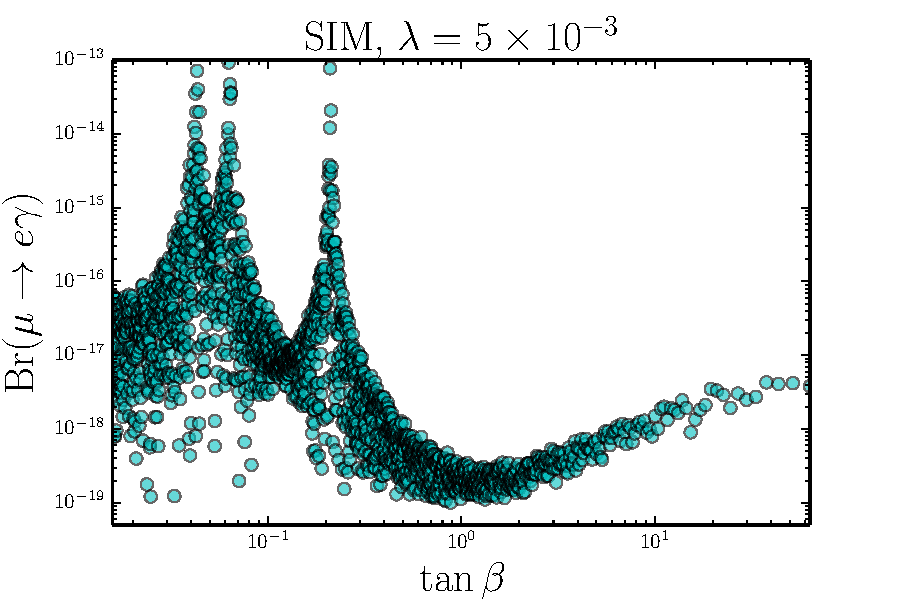
\includegraphics[scale=0.58]{brmuegammatanb}
\caption{$\tan\beta$ dependence of (a) $\Lambda_a$ and (b) $\operatorname{Br}(\mu \rightarrow e \gamma)$, for the set of input masses in eq.~\eqref{eq:bp} with
$\lambda=\num{5E-3}$.}
\label{fig:Lambdaa}
\end{figure}

%%%%%%%%%%%%%%%%%%%%%%%%%%%%%%%%%%%%%%%%%%%%%%%%%%%%%%%%%%%%%%%%%%%%%%%%%%%%%%%%%%%%%%%%%%%%%%%%%%%%
\section{Lepton flavor violation}
\label{sec:lept-flav-viol}

The size of the lepton flavor violation (LFV) is controlled by the lepton
number violating couplings $h_{i\alpha}$.  
From the approximate expression for $\Lambda_{\alpha}$
in~\eqref{eq:lambdaappr} and the analysis of the previous section, we
will show that these couplings are inversely related to the Yukawa
coupling strength $\lambda$.
Since in SDFDM the observed dark matter abundance is typically
obtained for $\lambda\gtrsim 0.1$~\cite{Cheung:2013dua}, the lepton
flavor observables are not expected to give better constraints than
the obtained from direct detection experiments. Therefore, we will
focus our discussion of LFV in regions of the parameter space
where $S_1$ is the dark matter candidate.

\begin{figure}[h]
\label{fig:muegamma}
\centering
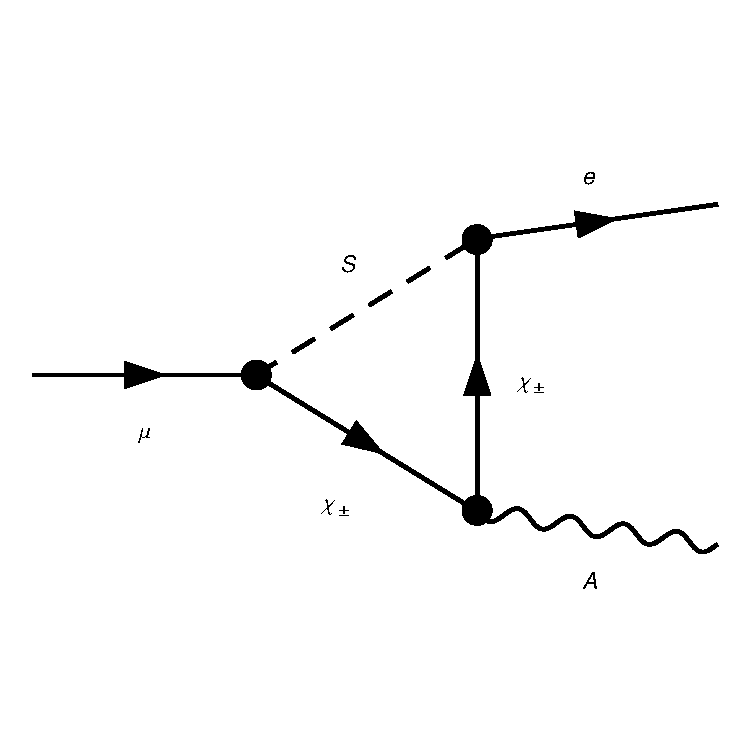
\includegraphics[scale=0.45]{t13a-muegamma1}
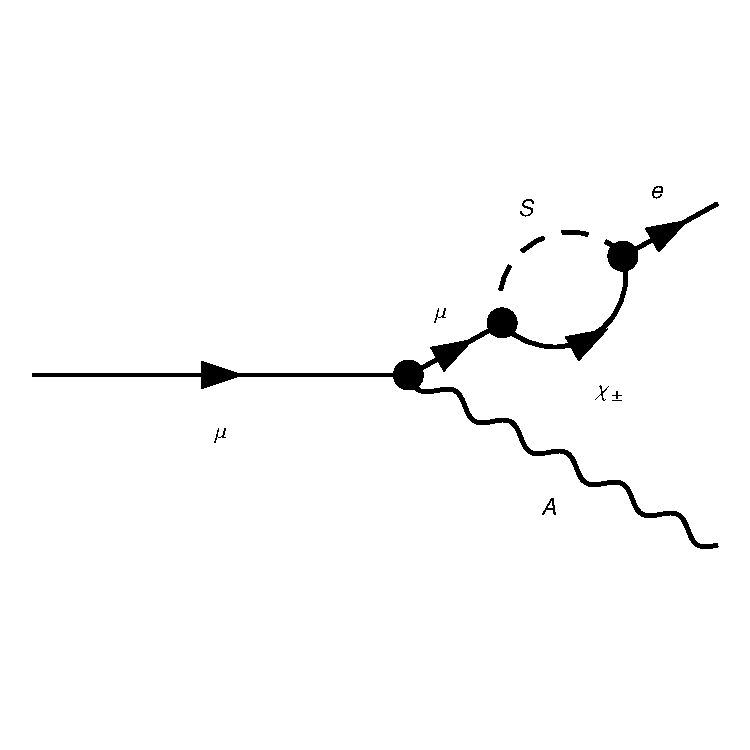
\includegraphics[scale=0.45]{t13a-muegamma2}
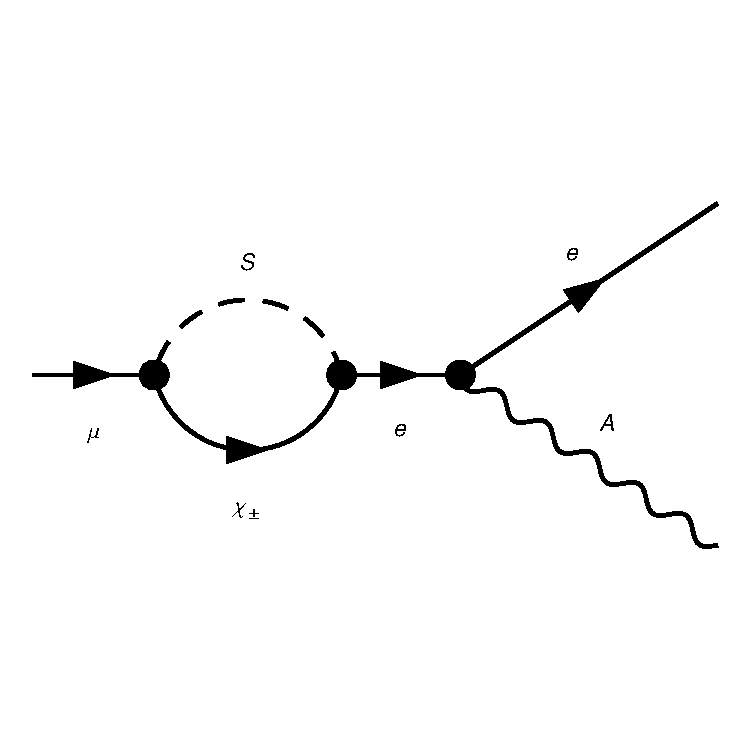
\includegraphics[scale=0.45]{t13a-muegamma3}
\caption{$\mu \to e \gamma$ process generated using \textsc{FeynArts}~\cite{Hahn:2000kx}.}
\end{figure}

It is well known that LFV processes put severe constraints on the LFV
couplings and, in general, on the model's parameter space. 
One of the most restrictive LFV processes is the radiative muon decay
$\mu\to e\gamma$, which in the present model is mediated by same
particles present in the internal lines of the one-loop neutrino mass
diagram, Fig.~\ref{fig:muegamma}. 
The corresponding expression for the branching ratio is computed in the Appendix~\ref{sec:Ap-muegamma}. It is given by
%
\begin{align}
\label{eq:muegamma}
\operatorname{Br}(\mu \rightarrow e \gamma)=&\dfrac{3}{4}\dfrac{\alpha_{\text{em}}}{16 \pi G_F^2}\left|\sum_{\alpha}
h_{1\alpha}\frac{F\left(M_D^2/m_{S_{\alpha}}^2  \right) }{m_{S_\alpha}^2}h_{2\alpha}^{*}  \right|^2 ,
\end{align}
where
\begin{align}
F(x)=\dfrac{x^3-6x^2+3x+2+6x\ln x}{6(x-1)^4}\,.
\end{align}
%
With the implementation of the model in the
\texttt{BSM-Toolbox}~\cite{Staub:2011dp} of
\texttt{SARAH}~\cite{Staub:2008uz,Staub:2013tta}, we have crosschecked
the one-loop results for both neutrino masses and $\operatorname{Br}(\mu
\rightarrow e \gamma)$.
Moreover, with the \texttt{SARAH}
\texttt{FlavorKit}~\cite{Porod:2014xia}, we have also checked that the
most restrictive lepton flavor violating process in the scan, to be
described below, is just Br($\mu\to e\gamma$).
%
From Eqs.~\eqref{eq:Mnuij} and~\eqref{eq:ht}, we obtain
\begin{align}
  M^{\nu}_{12}=\sum_{\alpha} h_{1\alpha} \Lambda_{\alpha}
  h_{2\alpha}=\left[ \mathbf{U}^{*}\mathbf{M}^{\nu}_{\text{diag}}\mathbf{U}^{\dagger} \right]_{12}\,.%=\sum_{j}m_{\nu j}U_{1j}^{*}U_{2j}^{*}\,.
\end{align}
Comparing this result with the corresponding combination of couplings
in the expression for Br$(\mu\to e\gamma)$ in Eq.~\eqref{eq:muegamma},
we expect that for a set of fixed input masses $\operatorname{Br}(\mu
\rightarrow e \gamma)$ turns out to be inversely proportional to
$\Lambda_\alpha^2$.
This is illustrated in Fig.~\ref{fig:Lambdaa}(b)
for $\lambda=\num{5E-3}$, where the scatter plot of
$\operatorname{Br}(\mu\to e \gamma)$ is shown for the same range of $\tan\beta$ values 
 than in Fig.~\ref{fig:Lambdaa}(a).  In such a case, once
$h_{i\alpha}$ are obtained from the Casas-Ibarra parametrization, the
specific hierarchy of $\Lambda_{\alpha}$ fixes the several contributions
to $\operatorname{Br}(\mu \rightarrow e \gamma)$.  The dispersion of
the points is due to the 3-$\sigma$ variation of neutrino oscillation
data~\cite{Forero:2014bxa} used in the numerical implementation of the Casas-Ibarra
 parametrization, along with the random variation of the parameters of
$\boldsymbol{\mathcal{R}}$. The minimum value of
$\operatorname{Br}(\mu \rightarrow e \gamma)$ around $\tan\beta=1$
corresponds to the maximum value of $\Lambda_{\alpha}$, while the
maximum values happen at the cancellation points of each
$\Lambda_{\alpha}$. In the subsequent analysis, and for a fixed SIM and $\lambda$, we allow 
for cancellations only by two orders of magnitude from the maximum
value of each $\Lambda_{\alpha}$. 

The full scan of the input masses up to $\SI{2}{TeV}$, with
$m_{S_1}>\SI{53}{GeV}$~\cite{Abe:2014gua} as the dark matter candidate,
$M_D>\SI{100}{GeV}$ to satisfy LEP constraints, and
$10^{-2}\le\tan\beta\le 10^2$, give to arise the dark-gray plus
light-gray regions in Fig.~\ref{fig:brmuegamma}. In particular, the
$\lambda$ variation for the SIM with $\beta=\pi/6$, denoted by yellow
stars in Fig.~\ref{fig:Lambdaa}(a), is illustrated
with the white dots in Fig.~\ref{fig:brmuegamma}.   The
corresponding dashed line is obtained for the best-fit values of the
neutrino oscillation data and $\boldsymbol{\mathcal{R}}$ fixed to the
identity. The horizontal dotted line in the plot corresponds to the
current experimental bound for $\operatorname{Br}(\mu\to e
\gamma)<\num{5.7E-13}$ at $90\%\,\si{CL}$~\cite{Adam:2013mnn}.  
The upper part of the 
light-gray region is restricted by our imposition to avoid too strong
cancellation in  $\Lambda_{\alpha}$ . We check that for all the sets of
input masses in the random scan, this cancellation region always
happens when $\tan\beta<1$. In this way, points with $\tan\beta>1$ are
absent from the light-gray region, as labeled in
Fig.~\ref{fig:brmuegamma}. For the same reason, in the dark-gray
region there are not points with $\Lambda_{\alpha}\ll
\Lambda_{\beta}\sim \Lambda_\gamma$ ($\alpha\ne\beta\ne\gamma$). We can check for example that
points with $\Lambda_1\ll \Lambda_2<\Lambda_3$ are absent inside the
dark-gray region of Fig.~\ref{fig:brmuegamma}.


\begin{figure}
  \centering
  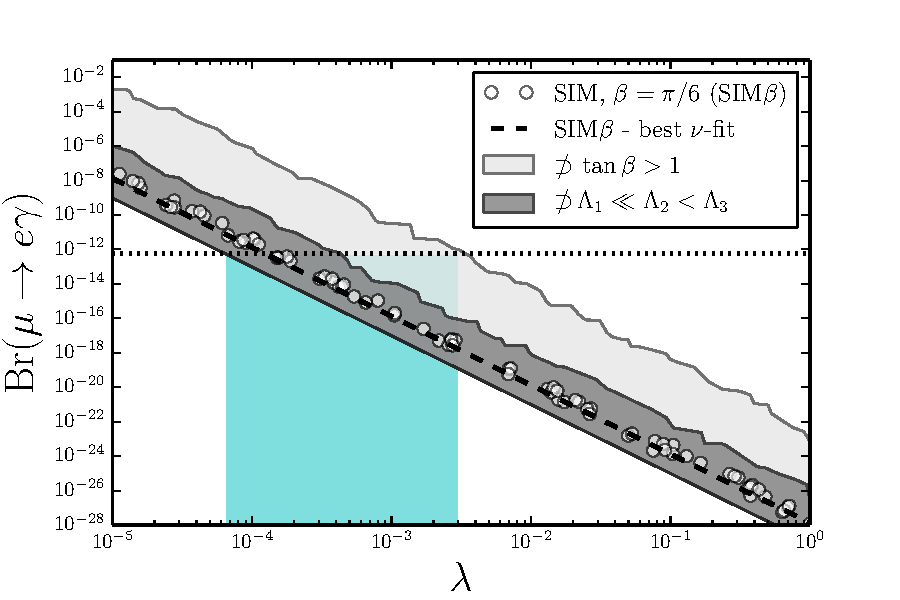
\includegraphics[scale=0.7]{brmuegamma}
  \caption{$\operatorname{Br}(\mu \rightarrow e \gamma)$ in terms of
    the Yukawa coupling strength $\lambda$ for the SIM in
    Eq.~\eqref{eq:bp} with $\beta=\pi/6$, and the general scan
    described in the text.}
  \label{fig:brmuegamma}
\end{figure}



The lower part of the dark-gray region is saturated by the values of
$M_{D}=\SI{2}{TeV}$, and gives rise to the lower bound $\lambda\gtrsim
\num{6E-5}$. 
With our restriction in the cancellation of
$\Lambda_{\alpha}$,  points in the scan with $\lambda\lesssim\num{3E-3}$ 
can be excluded from the Br$(\mu\to e\gamma)$ limit.    


\section{Collider phenomenology}
\label{sec:collider-phenomenology}

The LHC phenomenology in the case of the singlet-doublet fermion
dark matter was already analyzed in~\cite{Abe:2014gua}. They concluded that
the recast of the current LHC data is easier to evade, but the
long-run prospects are promising, since the region $M_N,m_\lambda\ll M_D$ could be 
probed up to $M_D\lesssim 600-\SI{700}{GeV}$ for the 14-TeV run of the LHC with 
$\SI{3000}{fb}^{-1}$. 

On the other hand, in the case of the singlet scalar dark matter, the
main production processes associated with the new fermions remain the
same, but there are new signals from the mediation, or presence in the
final decay chains, of the new scalars.
The most promising possibility is the dilepton plus missing
transverse energy signal coming from the production of
charged fermions decaying into leptons and the lightest scalar.
This signal can be important when $\lambda$ is
not too large, $\lambda\lesssim 0.1$, and $M_N\gtrsim M_D$. 
For a fixed set of input parameters, the random phases in the
Casas-Ibarra can be chosen to have all the possibilities in the lepton
flavor space associated with the coupling $h_{i1}$, with
$i=e,\mu,\tau$. 
In view of that, we will focus in the best scenario where
$\operatorname{Br}(\chi^\pm\to l^\pm \, S_1 )\approx 1$ ($l^\pm=e^\pm$ or
$\mu^\pm$). 
The Feynman diagram for the processes is displayed in
Fig.~\ref{fig:chain_signal}.

   
The mass of the  charged  Dirac fermion $\chi^{\pm}$, can be
constrained from dilepton plus missing transverse energy  searches at the  LHC.
In~\cite{Aad:2014vma}, this kind of signals was used by the ATLAS
collaboration to establish bounds on the slepton masses from the
search for $pp \rightarrow \tilde{l}^+\tilde{l}^- \rightarrow l^+l^-
\tilde{\chi}^0\tilde{\chi}^0$, where $\tilde{\chi}^{0}$ are the neutralinos,
and the same exclusion is reported for $l=e$ or $\mu$.
Purely left-handed sleptons produced and decaying this way, have been
excluded up to masses of about $300$ GeV at 95\% CL, from the data
with integrated luminosity of 20.3 fb$^{-1}$ and the $pp$ collision
energy of 8 TeV. 
This corresponds to an excluded cross section of $\SI{1.4}{fb}$ at NLO
calculated with \texttt{PROSPINO}~\cite{Beenakker:1996ed}.

In the present model, the charged fermion field may decay in the
mode $\chi^{\pm} \rightarrow e_i^{\pm}S_1$ which are
proportional to the Yukawa couplings $h_{i1}$. 
Therefore, a similar final state as in the slepton pair production is
obtained through the process $pp \rightarrow \chi^+\chi^- \rightarrow
l^+l^- S_1 S_1$, as can be seen in Fig.~\ref{fig:chain_signal}.


\begin{figure}[h]
\begin{center}
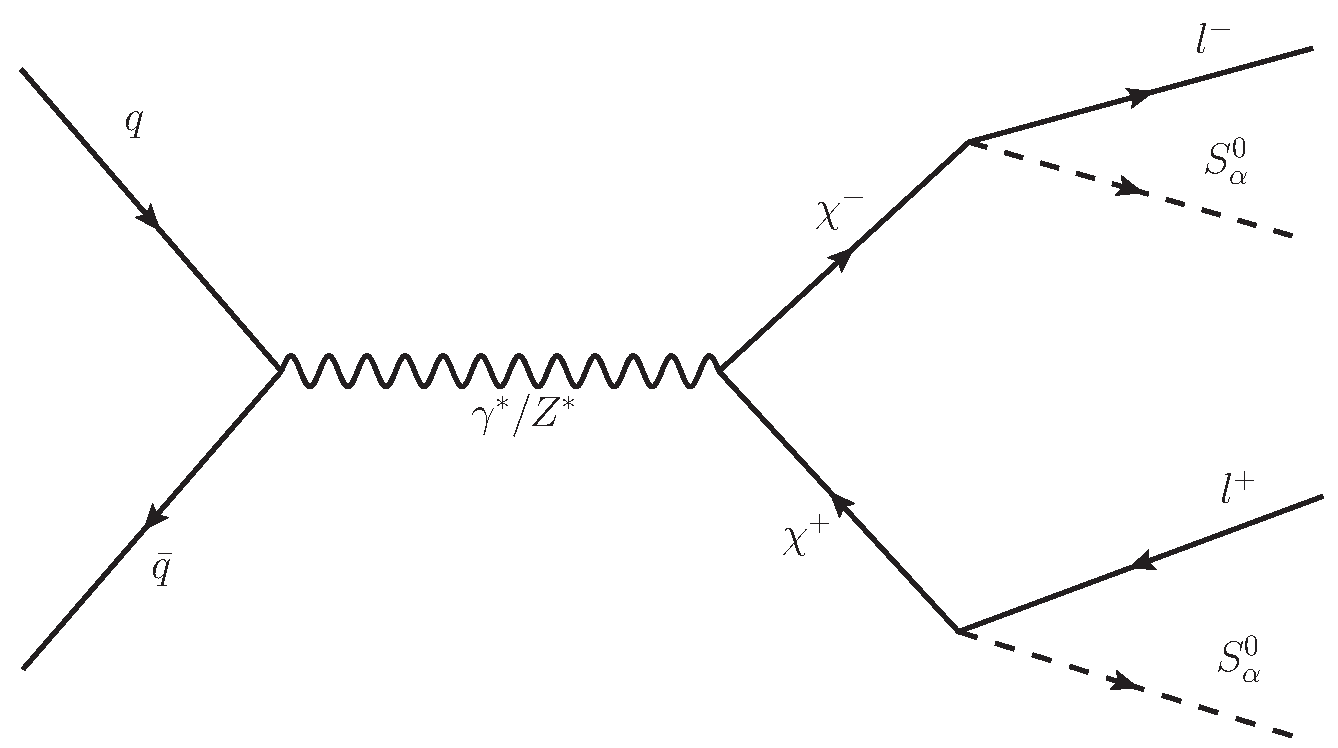
\includegraphics[scale=0.4]{chain1}
\caption{Feynman diagram for $pp \rightarrow \chi^+\chi^- \rightarrow l^+l^- S_{\alpha}S_{\alpha}$ (Drell-Yan process).}
\label{fig:chain_signal}
\end{center}
\end{figure}

In this case, the excluded cross section of this process can be estimated from:

\begin{align}
\label{eq:exccs}
\sigma(pp \rightarrow l^+l^-S_1 S_1)=\sigma(pp \rightarrow \chi^+\chi^-)\times \operatorname{Br}(\chi^{\pm} \rightarrow l^{\pm}S_1)^2 ,
\end{align}
where $\sigma(pp \rightarrow \chi^+\chi^-)$ is the pair production
cross section of charged Dirac fermion, and
$\operatorname{Br}(\chi^{\pm} \rightarrow l^{\pm}S_1)$ is the
branching fraction for $\chi^{\pm} \rightarrow l^{\pm}S_1$
mode.

The pair production of charged Dirac fermions can be
calculated in the pure-higgsino limit of the minimal supersymmetric
standard model. 
The NLO cross section calculated with \texttt{PROSPINO} is displayed
in Fig.~\ref{fig:chargino_production} as a function of the charged
Dirac fermion.

For points in the parameter space where the Casas-Ibarra solution is
chosen such that $\operatorname{Br}(\chi^\pm\to l^\pm\,S_1)\approx 1$,
and assuming the same efficiency as for the dilepton plus missing
transverse energy signal coming from left-sleptons in
Eq.~\eqref{eq:exccs}, the charged Dirac fermions of the present model
can be excluded up to $\SI{510}{GeV}$, as illustrated in
Fig.~\ref{fig:chargino_production}.

\begin{figure}[h]
\begin{center}
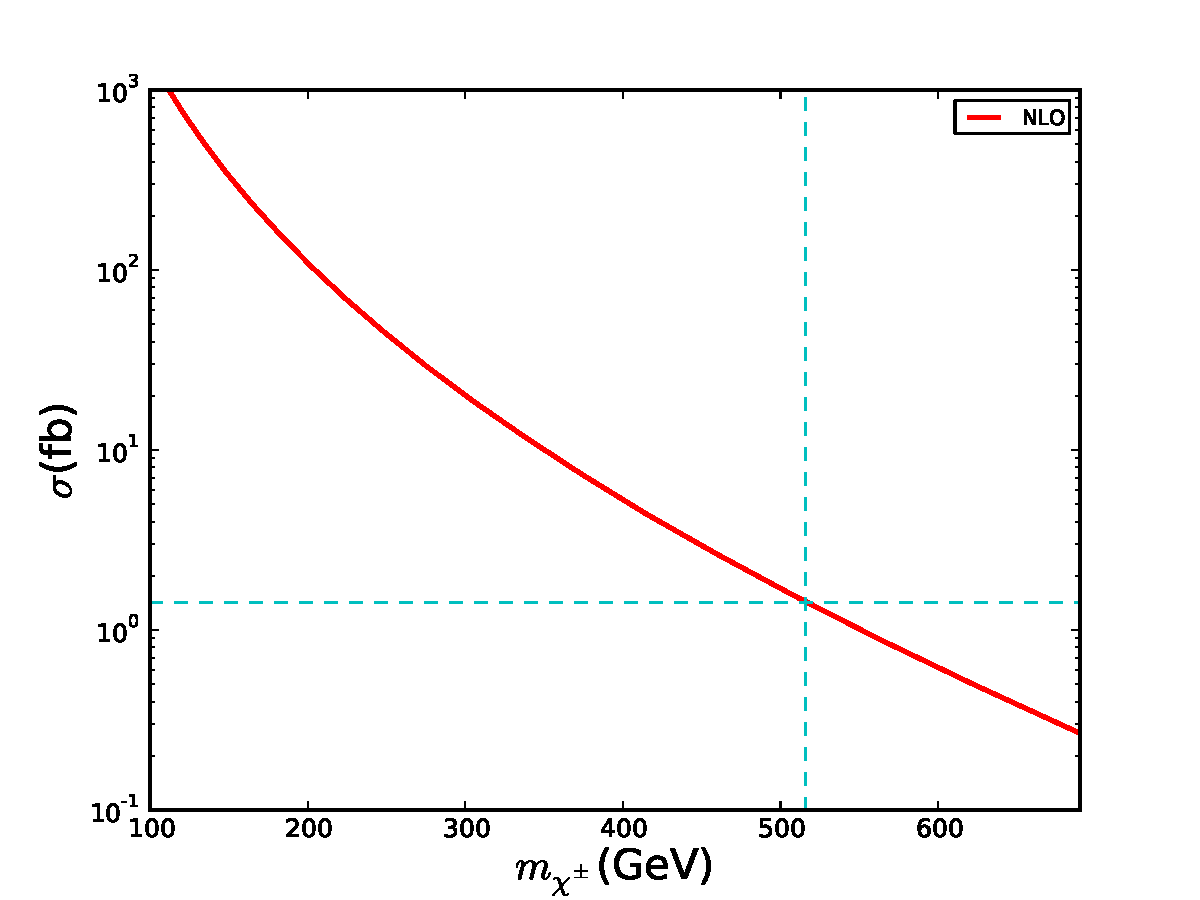
\includegraphics[scale=0.5]{cs2_chacha_prospino}
\caption{NLO cross section for the charged Dirac fermion pair
  production at the LHC with $pp$ collisions at $\sqrt{s}=8$ TeV. 
  The horizontal dashed line for the excluded cross section of
  $\SI{1.4}{fb}$, corresponds to the mass about $\SI{510}{GeV}$
  illustrated by the vertical dashed line.}
\label{fig:chargino_production}
\end{center}
\end{figure}

Note that many points in the scan of Fig.~\ref{fig:brmuegamma} with
$\lambda\lesssim 0.1$ and featuring $m_{S_1}\ll M_D$, could be
excluded by this LHC constraint. 
However, a detailed analysis of the restriction from the Run~I of the
LHC, in the full parameter space of the model, is beyond the scope of this
work.

\section{Coannihilation in the SDFDM model}
\label{sec:singlet-doublet-dark}
In this model, the role of the dark matter particle can be played by
either the lightest of the fermions $\chi_{\text{LOP}}$ or the lightest of the
scalars $S_1$. 
In the latter case, the present model resembles the
singlet scalar DM model
\cite{Silveira:1985rk,McDonald:1993ex,Burgess:2000yq} as long as the
other $Z_2$-odd particles do not contribute to the total annihilation
cross section of $S_1$, namely through to the addition of new
(co)annihilation channels. 
Therefore, by choosing a non-degenerate mass spectrum and small Yukawa
couplings (which is in agreement with neutrino masses) the effects of these particles on dark matter can be neglected. 
Hence, we expect that the dark matter phenomenology to be similar to
that of the SSDM \cite{Cline:2013gha}. 

On the other hand, regarding the case of fermion DM, the present model includes the
singlet doublet fermion DM model
\cite{ArkaniHamed:2005yv,Mahbubani:2005pt,D'Eramo:2007ga,Enberg:2007rp,Cohen:2011ec,Cheung:2013dua}.
In such a scenario, when the dark matter candidate is mainly singlet
(doublet), the relic density is in general rather large (small). 
In particular, a pure doublet has the proper relic density for
$M_{D}\sim\SI{1}{TeV}$~\cite{Mahbubani:2005pt,Cheung:2013dua,Chattopadhyay:2005mv}
with decreasing  values as $M_D$ decreases.  
Nonetheless, in the present model we have the additional possibility
of coannihilations between the $Z_2$-odd scalars and fermions. 
In this work, we explore at what extent coannihilation with
scalars may allow to recover pure-doublet DM regions with
$M_D\lesssim\SI{1}{TeV}$ and $\lambda\lesssim0.3$, while keeping the
proper relic density.  
Hereafter, we focus in that specific region.


In the simple radiative seesaw model with inert
doublet scalar dark matter, the coannihilations with singlet fermions can enhance
rather than reduce the relic density, as shown in~\cite{Klasen:2013jpa}. That work also presented a review of the several
models~\cite{Servant:2002aq,Kong:2005hn,Burnell:2005hm,Edsjo:2003us,Profumo:2006bx}
where such an enhancement also occurs.
In particular, supersymmetric models where
the neutralino is higgsino-like were considered in~\cite{Profumo:2006bx} and it
was shown that slepton coannihilations not only lead to an increase in
the relic density but also to an enhancement in the predicted
indirect detection signals. 
Below, we show that the singlet scalars can play the role of the
sleptons in our generalization of the higgsino-like dark matter with
radiative neutrino masses.


\begin{figure}
  \centering
  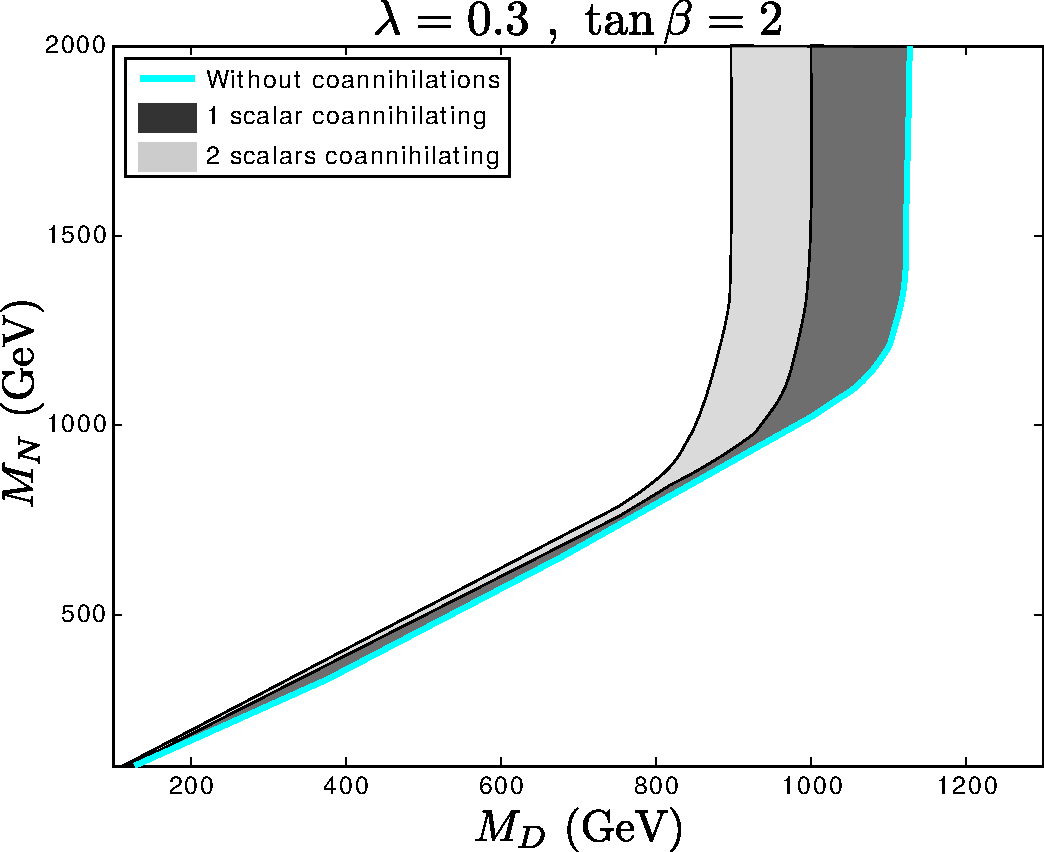
\includegraphics[scale=0.5]{sdfdm}
  \caption{Regions consistent with the observed relic density for $\lambda=0.3$
   and $\tan\beta=2$.    The solid cyan line corresponds to the observed relic density
   without coannihilations which were shown to be compatible with the
   current direct detection bounds from LUX~\cite{Akerib:2013tjd}
   in~\cite{Cheung:2013dua}.
   The effect of the coannihilations with the new scalars is shown for
   a mass degeneracy of 0.1 to 10\% between the scalars and the DM
   candidate. 
   The dark-gray region corresponds to coannihilations with one scalar
   singlet, while the dark plus light-gray regions correspond to
   coannihilations with two scalar singlets.  }
  \label{fig:5b}
\end{figure}


The interactions of the scalars $S_\alpha$ are described by the
$h_{i\alpha}$, $\lambda_{\alpha\beta}^{SH}$ terms in
Eq.~\eqref{eq:lt13a}. 
It turns out that Yukawa interactions are suppressed by neutrino
masses ($h_{i\alpha}\lesssim10^{-4}$) and the same occurs for the interaction
with the Higgs boson if we impose
$\lambda_{\alpha\beta}^{SH}\lesssim10^{-2}$.
In this way, the coannihilating scalars $S_\alpha$ act as parasite
degrees of freedom at freeze-out, leading to an increase of the
singlet-doublet fermion relic density. 

By following the discussion in~\cite{Klasen:2013jpa}, the maximum
enhancement of the relic density is achieved when
$\Delta_{S_\alpha}=(m_{S_{\alpha}}-m_{\text{LOP}}^{\chi})/m_{\text{LOP}}^{\chi}$
becomes negligible. 
Accordingly, one can write
\begin{align}
\frac{  \Omega^{S_{\alpha}}}{\Omega^{0}}\approx\left( \frac{g_0+g_{S_{\alpha}}}{g_0} \right)^2,
\end{align}
where $\Omega^{S_{\alpha}}$ ($\Omega^{0}$) denotes the relic density
with (without) including $S_{\alpha}$ coannihilations,
$g_{S_{\alpha}}$ represents the total number of internal degrees of
freedom related to the scalars participating in the in the
coannihilation process, and $g_{0}$ is the total number of internal
degrees of freedom when $\Delta_{S_\alpha}\gg1$. 
When the DM particle is pure doublet ($M_D\sim1$ TeV and $M_N\gg M_D$),
the fermion masses are $m_1^{\chi}=M_N,\,m_{2,3}^{\chi}\approx
m_{\chi^\pm}=M_D$ and therefore
$g_{0}=g_{\chi_2}+g_{\chi_3}+g_{\chi^\pm}=8$.
Since each real scalar has one degree of freedom, we have
$g_{S_{\alpha}}=1,2,3$ depending on the number of scalars
coannihilating. Thus, it follows that the maximum enhancement is
$\Omega^{S_{\alpha}}/\Omega^{0}=1.27,\, 1.56,\,1.89$, respectively. 
This enhancement results in that, for the present model with
doublet-like DM and $\lambda\lesssim0.3$, the $M_D$ required to explain
the correct relic density lies in the range $[0.9,1.1]$~TeV instead of
taking a single value as in the SDFDM model.  
The values inside this range arise due to no mass-degeneracy
between the fermions and scalars. 
In Fig.~\ref{fig:5b}, we show the effect of coannihilations on the
relic density~\footnote{The relic density is calculated with the
  \texttt{BSM-Toolbox} chain: 
\texttt{SPheno}~3.3.6~\cite{Porod:2011nf}-\texttt{MicrOMEGAs}~4.1.7~\cite{Belanger:2006is,Belanger:2014vza}.}
of $m_{\text{LOP}}^{\chi}$ for a mass degeneracy of 0.1
to 10\% between  scalar singlets and the DM candidate and for
$\lambda=0.3$ and $\tan\beta=2$. 
In particular, in the light-gray region we plot the coannihilations
with two scalars to facilitate the comparison with the results
in~\cite{Profumo:2006bx} for higgsino-like dark matter coannihilating
with a right-handed stau ($g\approx 2$ in their plots).
As expected, the upper limit in the LOP mass is about $20\%$ smaller
with respect to the case without coannihilation, and we could 
expect similar enhancements for indirect DM searches
as  in ~\cite{Profumo:2006bx} for $g\approx 2$.
Note that, when $M_D,\,M_N<\SI{1}{TeV}$, the impact of the $S_\alpha$ coannihilation is reduced because, in such case, the
dark matter particle is a mixture of singlet and doublet
(well-tempered DM \cite{ArkaniHamed:2006mb}), and the non-negligible
splitting among the fermion particles $\chi$ leads to a non-zero
Boltzmann suppression. 
We have checked that the same results are obtained when
$\lambda\lesssim0.3$.

With regard to DM direct detection in the pure-doublet DM scenario
discussed above, it is not restricted by the current LUX~\cite{Akerib:2013tjd} bounds as
long as $\tan\beta>0$.  
This is due to the existence of zones, known as blind spots, where the
spin-independent cross section vanishes identically and they occur
only for positive values of $\tan\beta$
\cite{Cheung:2013dua}\footnote{Note that $\tan\beta>0$ corresponds to
  $\tan\theta<0$ in notation of  \cite{Cheung:2013dua}.}. 
In consequence, the recovered pure-doublet DM regions are still viable
in light of the present results of direct searches of dark matter.  
%%%%%%%%%%%%%%%%%%%%%%%%%%%%%%%%%%%%%%%%%%%%%%%%%%%%%%%%%%%%%%%%%%%%%%%%







%
%\chapter{The \textit{Fermi}-LAT gamma-ray excess at the Galactic Center in the singlet-doublet
%fermion dark matter model}
%\begin{flushright}
This chapter in based in our work publish in \textbf{JCAP03(2016)048}\\ 
\url{doi.org/10.1088/1475-7516/2016/03/048}
\end{flushright}
\begin{center}
\textbf{Abstrac}
\end{center}
The singlet-doublet fermion dark matter model (SDFDM) provides a good DM candidate as well as the possibility of generating neutrino masses radiatively.
 The search and identification of DM requires the combined effort of both indirect and direct DM detection experiments in addition to the LHC.
 Remarkably, an excess of GeV gamma rays from the Galactic Center (GCE) has been measured with the \textit{Fermi}  Large Area Telescope (LAT) which appears to be robust with respect to changes in the diffuse galactic background modeling.
 Although several astrophysical explanations have been proposed, DM remains a simple and well motivated alternative.
 In this work, we examine the sensitivities of dark matter searches in the SDFDM scenario using \textit{Fermi}-LAT, CTA, IceCube/DeepCore, LUX, PICO and LHC with an emphasis on exploring the regions of the parameter space that can account for the GCE.
 We find that DM particles present in this model with masses close to $\sim 99$ GeV and $\sim (173-190)$ GeV annihilating predominantly into the $W^+W^-$ channel and $t\bar{t}$ channel respectively, provide an acceptable fit to the GCE while being consistent with different current experimental bounds. We also find that much of the obtained parameter space can be ruled out by future direct search experiments like LZ and XENON-1T, in case of null results by these detectors. Interestingly, we show that the most recent data by LUX is starting to probe the best fit region in the SDFDM model.

\section{Introduction to the Galactic Center Excess (GCE)}
%
WIMP particles appear effortlessly in many extensions of the SM that resolve outstanding theoretical and phenomenological problems which are not necessarily related to the DM puzzle.
 In some of these models, WIMPs can be produced in high energy colliders (collider DM searches), elastically scatter off nuclei (direct DM searches) or annihilate and produce observable particles in astrophysical environments (indirect DM searches).
 High-energy photons in the gamma-ray ($\gamma$-ray) frequency is the most notable search channel of the later category, as they can travel almost unperturbed from their sources to the detectors.
 The Large Area Telescope on board the \textit{Fermi} satellite (\textit{Fermi}-LAT)~\cite{Fermi} is the most sensitive $\gamma$-ray detector in the few GeVs energy range.

At the bottom of the gravitational well of the Milky Way Galaxy, the Galactic Center (GC) is expected to be the region displaying the brightest emission of DM annihilations in the $\gamma$-ray sky~\cite{Funk:review}.
 However, a multitude of non-thermal astrophysical sources present in that region complicate the identification of a tentative DM signal~\cite{Funk:review}. Observations of the inner few degrees around the GC with the \textit{Fermi}-LAT have revealed an excess of $\gamma$-rays ~\cite{Goodenough2009gk,Vitale:2009hr,Hooper:2010mq,hooper,AbazajianKaplinghat2012,AbazajianKaplinghat2013,GordonMacias2013}. 
The spectrum of the Galactic Center excess (GCE) peaks at about 1-3 GeV and its spatial morphology is spherically symmetric varying with radius $r$ around the GC as $r^{-2\gamma}$ with  $\gamma\sim 1.2$ which is clearly compatible with the DM density profile. 
This emission has been found to extend out in Galactic latitude ($b$) up to about $|b|\lesssim 20^\circ$ ~\cite{hooperslatyer2013,Daylan:2014,CaloreCholisWeniger2015,TheFermi-LAT:2015kwa} and its presence appears  to be robust with respect to systematic uncertainties~\cite{GordonMacias2013,MaciasGordon2014,Daylan:2014,Zho2015,CaloreCholisWeniger2015,PorterMurgia2015,TheFermi-LAT:2015kwa}.

In the Fig.~\ref{fig:GCE-less2} we show the GCE observed for $|b|<2^{\circ}$ and Galactic longitude $|l|<2^{\circ}$. This is the remaining excess after subtracting the Gamma Diffuse Emission of gamma rays (GDE) generate by cosmic rays that generate pions $\pi^0$ in collisions with the interstellar gas that latter decay and produce photons, by cosmic rays electrons that produce photon by bremsstrahlung emission and by photons accelerate by Inverse Compton scattering (ICS).
In the Fig.~\ref{fig:GCE-bigger2} we show all the completed signal observed of the Galaxy for   $|b|>2^{\circ}$ and the remaining GCE after clean the map using the best GDE models. 

\begin{figure}[h]
\begin{center}
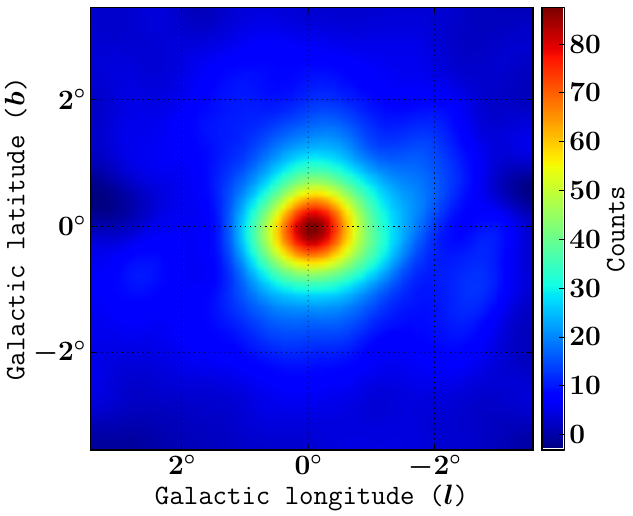
\includegraphics[scale=0.4]{latitude-less2}
\end{center}
\caption{Residual map or GCE signal~\cite{GordonMacias2013} for $|b,l|<2^{\circ}$. The counts were summed over the energy range 
$300$ MeV-$10$ GeV. The map spans a $7^{\circ}\times 7^{\circ}$ region of the sky centred in the Sgr A$^*$ position with a pixel size of $0.1^{\circ}\times 0.1^{\circ}$.}
\label{fig:GCE-less2}
\end{figure}
%
\begin{figure}[h]
\begin{center}
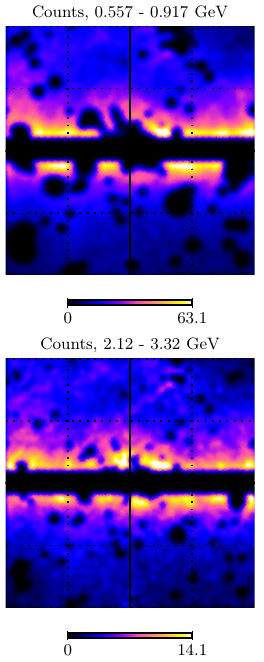
\includegraphics[scale=0.6]{latitude-bigger2a}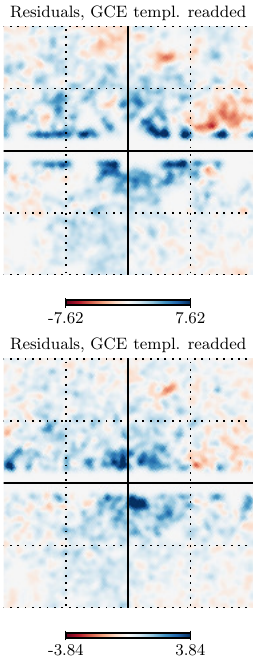
\includegraphics[scale=0.6]{latitude-bigger2b}
\end{center}
\caption{\textit{Left panels}: Counts map a various energies, with the disk cut $|b|>2^{\circ}$. \textit{Right panels}: Residual after sustracting the best Gamma Difuse emition model (GDE)~\cite{CaloreCholisWeniger2015}.}
\label{fig:GCE-bigger2}
\end{figure} 
 

There is an ongoing and intense debate as to what the origin of this signal is. A tentative explanation is an unresolved population of $\sim 10^3$ millisecond pulsars (MSPs)~\cite{Abazajian:2010zy,AbazajianKaplinghat2012,Wharton2012,GordonMacias2013,GordonMacias2013erratum,Mirabal2013,MaciasGordon2014,YuanZhang2014,BrandtKocsis2015,Lacroix:2015wfx,O'Leary:2016osi} or young pulsars \cite{OLeary2015,O'Leary:2016osi}.
 Nevertheless, some studies~\cite{Hooper2013,CholisHooperLinden2015,PetrovicSerpicoZaharijas2015,Lee2015,BartelsKrishnamurthyWeniger2015,Linden2015} have pointed out about the difficulties of reconciling this hypothesis with the GCE extending out as far as $\sim 10^\circ$ from the GC. On the other hand, recent works claim that the GCE is not smooth~\cite{Lee:2015fea,Bartels:2015aea}, and if confirmed, this would lend support to the MSPs alternative.
 Another scenario put forward is a series of energetic cosmic-ray injections in the GC \cite{CarlsonProfumo,Petrovic2014}.
 However, if the injected particles are mainly protons, it has been shown~\cite{MacGorCroProf2015} that this scenario is incompatible with the spatial morphology of the GCE in the inner $\sim 2^\circ$ of the Galaxy.
 In case the burst events contain protons as well as leptons, Ref~\cite{Cholis2015} finds suitable models that appear fine-tuned.

Despite these astrophysical uncertainties, a DM interpretation of the GCE cannot be ruled out yet~\cite{Goodenough2009gk,Hooper:2010mq,hooper,AbazajianKaplinghat2012,AbazajianKaplinghat2013,GordonMacias2013,MaciasGordon2014,Abazajian2014,Daylan:2014,Lacroix:2015wfx}.
   In this context, the spatial morphology of the GCE can be accommodated with a Navarro-Frenk-White (NFW) profile with a mildly contracted cusp of $\gamma\sim 1.2$, the measured spectrum implies a WIMP mass in the GeV energy range and an interaction cross section that coincides with the thermal relic cross section. 

A recent study of the GCE~\cite{CaloreCholisWeniger2015} selected a target region ($|b|>2^\circ$) that excluded the core of the GC. Additionally, the systematic uncertainties in the Galactic diffuse emission were estimated in a manner that made the low and high energy tails of the spectrum more uncertain than in previous analyses~\cite{GordonMacias2013,MaciasGordon2014,Abazajian2014,Daylan:2014}, which focused on a smaller region containing the inner $\sim 2^\circ$ of the GC. Although it is possible that the greater degree of uncertainty in the tails found by~\cite{CaloreCholisWeniger2015} is due to an intricate overlap of the GCE with the Fermi Bubbles~\cite{suslatyerfinkbeiner2010,Fermi-LAT:AnnaFranckowiak}, it is interesting that this uncertainty also allows much more freedom for DM models fitting the GCE~\cite{Logan:2010nw,Buckley:2010ve,Zhu:2011dz,Marshall:2011mm,Boucenna:2011hy,Buckley:2011mm,Anchordoqui:2013pta,Buckley:2013sca,Hagiwara:2013qya,Okada:2013bna,Huang:2013apa,Modak:2013jya,Boehm:2014hva,Alves:2014yha,Berlin:2014tja,Agrawal:2014una,Izaguirre:2014vva,Cerdeno:2014cda,Ipek:2014gua,Boehm:2014bia,Ko:2014gha,Abdullah:2014lla,Ghosh:2014pwa,Martin:2014sxa,Basak:2014sza,Berlin:2014pya,Cline:2014dwa,Han:2014nba,Detmold:2014qqa,Wang:2014elb,Chang:2014lxa,Arina:2014yna,Cheung:2014lqa,McDermott:2014rqa,Huang:2014cla,Balazs:2014jla,Ko:2014loa,Okada:2014usa,Ghorbani:2014qpa,Banik:2014eda,Borah:2014ska,Cahill-Rowley:2014ora,Guo:2014gra,Freytsis:2014sua,Heikinheimo:2014xza,Arcadi:2014lta,Richard:2014vfa,Cao:2014efa,Bell:2014xta,Cerdeno:2015ega,Caron:2015wda,Bertoneetal,Freeseetal}.  


Significant effort has been made in exploring the properties of DM models that can explain the GCE while being consistent with other indirect, direct and collider constraints~\cite{Logan:2010nw,Buckley:2010ve,Zhu:2011dz,Marshall:2011mm,Boucenna:2011hy,Buckley:2011mm,Anchordoqui:2013pta,Buckley:2013sca,Hagiwara:2013qya,Okada:2013bna,Huang:2013apa,Modak:2013jya,Boehm:2014hva,Alves:2014yha,Berlin:2014tja,Agrawal:2014una,Izaguirre:2014vva,Cerdeno:2014cda,Ipek:2014gua,Boehm:2014bia,Ko:2014gha,Abdullah:2014lla,Ghosh:2014pwa,Martin:2014sxa,Basak:2014sza,Berlin:2014pya,Cline:2014dwa,Han:2014nba,Detmold:2014qqa,Wang:2014elb,Chang:2014lxa,Arina:2014yna,Cheung:2014lqa,McDermott:2014rqa,Huang:2014cla,Balazs:2014jla,Ko:2014loa,Okada:2014usa,Ghorbani:2014qpa,Banik:2014eda,Borah:2014ska,Cahill-Rowley:2014ora,Guo:2014gra,Freytsis:2014sua,Heikinheimo:2014xza,Arcadi:2014lta,Richard:2014vfa,Cao:2014efa,Bell:2014xta,Cerdeno:2015ega,Caron:2015wda,Bertoneetal,Freeseetal}.
 Of great interest are the properties of minimal supersymmetric extensions of the SM (MSSM)~\cite{Cheung:2014lqa,Cahill-Rowley:2014ora,Cao:2014efa,Cerdeno:2015ega,Caron:2015wda,Bertoneetal,Freeseetal} that can fit the GCE.
 When these extensions are studied in light of the GCE extracted from the region $|b|>2^\circ$ of the GC, the required neutralino annihilation rates to mainly the $W^+W^-$ and $\bar{t}t$ channels are found to comply with the LEP or LHC bounds on sfermion masses.
 
 
Here, we do not restrict ourselves to supersymmetric models. Instead, we take the approach of studying a simplified DM model in which the DM candidate is a mixture, generated by the interaction with the Higgs boson, of a SM fermion singlet and the neutral components of an electroweak doublet vector-like fermion~\cite{ArkaniHamed:2005yv,Mahbubani:2005pt,D'Eramo:2007ga,Enberg:2007rp}. This model, also known as the singlet$-$doublet fermion DM (SDFDM) model, is one of the simplest UV realizations of the fermion Higgs portal ~\cite{Patt:2006fw} with the SM Higgs boson as the mediator between the visible and dark sectors. In fact, the dark sector of the SDFDM model (along with the stabilizing discrete symmetry) is part of the minimal setup expected when the SM is extended by new physics which is to some extent related to lepton and baryon number conservation~\cite{Arbelaez:2015ila,Arkani-Hamed:2015vfh}. While being free of many theoretical biases, this  model allows us to extract maximal phenomenological information from a framework that is a good representation of the WIMP paradigm \cite{ArkaniHamed:2005yv,Mahbubani:2005pt,D'Eramo:2007ga,Enberg:2007rp,Cohen:2011ec,Cheung:2013dua,Abe:2014gua,Calibbi:2015nha,Freitas:2015hsa,Abdallah:2015ter}\footnote{ If scalar singlets are added to its particle content, neutrino masses can also be radiatively generated in this generic class of models~\cite{Restrepo:2015ura}.}.     
Accordingly, the SDFDM model is set to become one of the models to be implemented in future searches for DM particles at the LHC \cite{Abdallah:2015ter} and a future 100 TeV hadron collider \cite{Gori:2014oua,Arkani-Hamed:2015vfh}.  


In this chapter, we examine the coverage of WIMP parameter space in the SDFDM model by using mainly indirect and direct DM search techniques in light of the recent detection of the GCE. We show the set of parameters in the SDFDM model that are compatible with the GCE while being consistent with current experimental bounds. Following the same methods explained in Ref.~\cite{Silverwood:2014yza} we compute the expected limits in the annihilation cross-section by the Cherenkov Telescope Array (CTA) and find that observations toward the GC by this instrument will not be able to confirm this model as an explanation of the GCE. However, we find that the viable models can be ruled out by future
direct search experiments such as LZ and XENON-1T, in the case of null results by these detectors. Interestingly, we show that the most recent data by LUX is starting to probe the best fit region in the SDFDM model.

\section{Self-annihilation channels in the high region of the SDFDM model}
\label{sec:modelgce}

In the SDFDM model, DM particles ($\chi^0$) can self-annihilate into $\bar{f}f$, $ZZ$, $W^+W^-$ and $hh$ final states through  $s$-channel Higgs and $Z$ boson exchange and into $ZZ$, $W^+W^-$ states via $t$-channel $\chi_i^0$ and $\chi^{\pm}$ exchange. Annihilations into a mixture of weak gauge bosons $Zh$ are also possible through the exchange of a $\chi_i\neq\chi^0$  in the $t$-channel or a $Z$ in the $s$-channel.  We remark in passing that gamma-ray lines $\gamma\gamma$ and $\gamma Z$ can also be produced at one-loop level. 

Of particular importance for indirect detection studies in this framework is the fact that since DM annihilations into fermion pairs mediated by the Higgs are $p$-wave suppressed (there is no $s$-wave amplitude), the annihilations produced through $Z$ exchange are dominant. We note that the later is also helicity suppressed, this implies that the main annihilation channel is the $t\bar{t}$ ($b\bar{b}$) for a dark matter mass above (below) the top mass, with $\langle\sigma v \rangle\lesssim 10^{-27}$ cm$^3$ s$^{-1}$ for $m_{\chi^0}<m_W$ \cite{Calibbi:2015nha}. In the case scenario of DM particles going into gauge bosons, we find that only those processes in the $t$-channel are relevant to our analysis as they do not suffer velocity suppression. Such a non-velocity suppression is also present in $s$ and $t$ channels for the annihilation into $Zh$. 
In contrast, we get that processes in which DM self-annihilates into a couple of Higgs bosons are velocity suppressed. 
At higher order in scattering theory the loop suppression leads to small values of the corresponding thermal cross sections \cite{Calibbi:2015nha}. One of the prime motivations of the present study is to explore the viable regions of the parameter space where the velocity averaged cross-section $\langle\sigma v\rangle$ can exhibit values comparable to those predicted by the WIMP paradigm (see Fig.~\ref{fig:good-sv}). It is in this sense that we will not consider DM annihilations into $\gamma\gamma,\gamma Z,hh$ and $ b\bar{b}$ in the discussion that follows.  

\begin{figure}[h]
\begin{center}
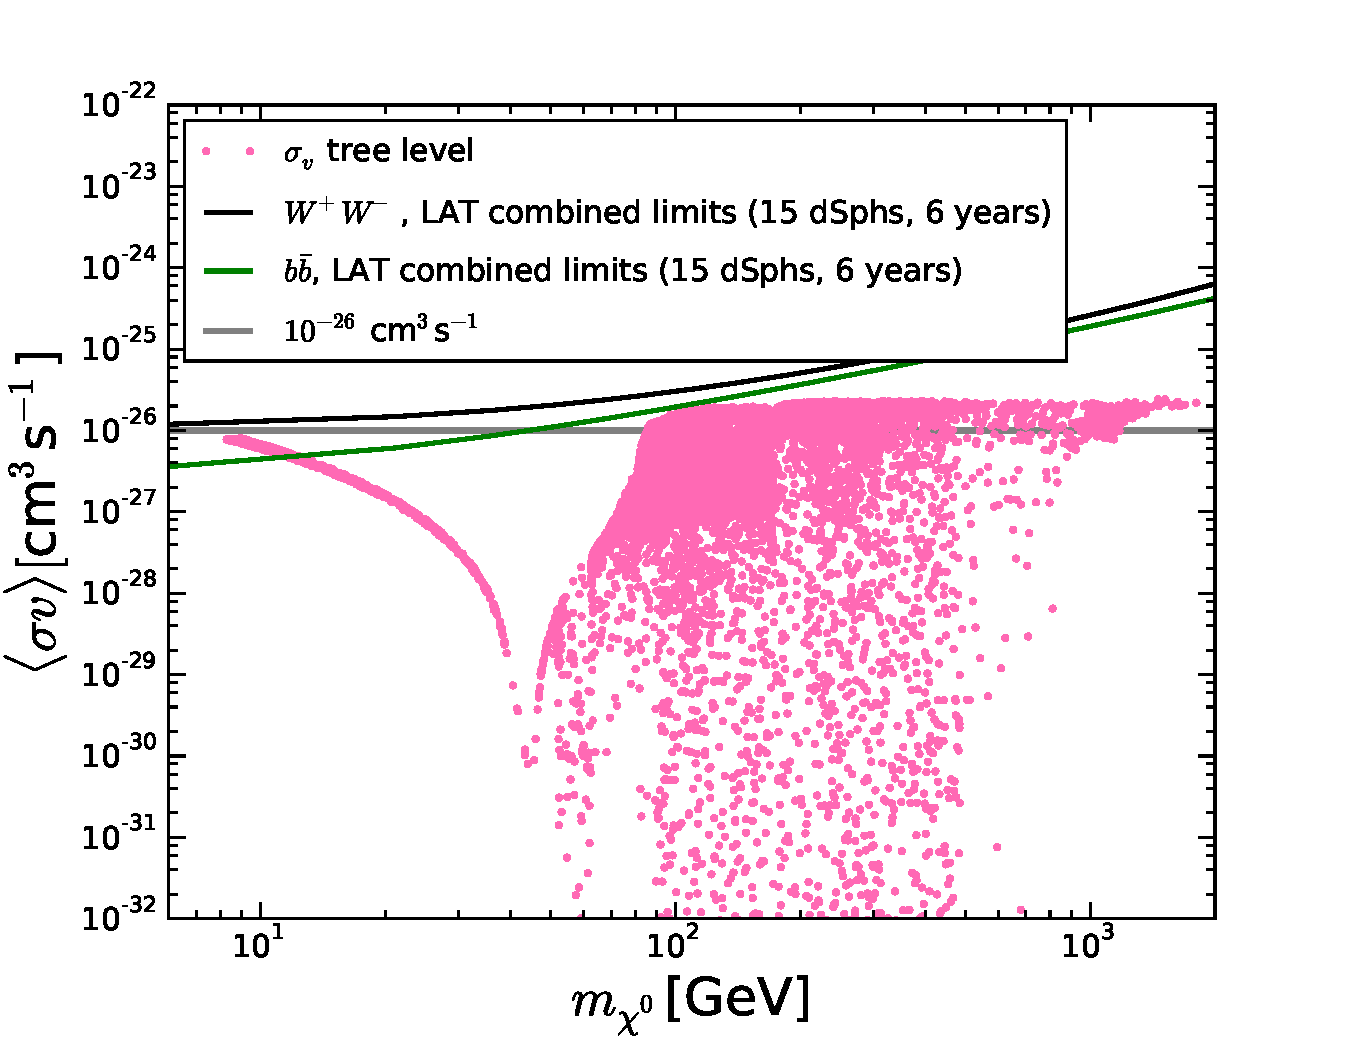
\includegraphics[scale=0.41]{sigmav-T13A}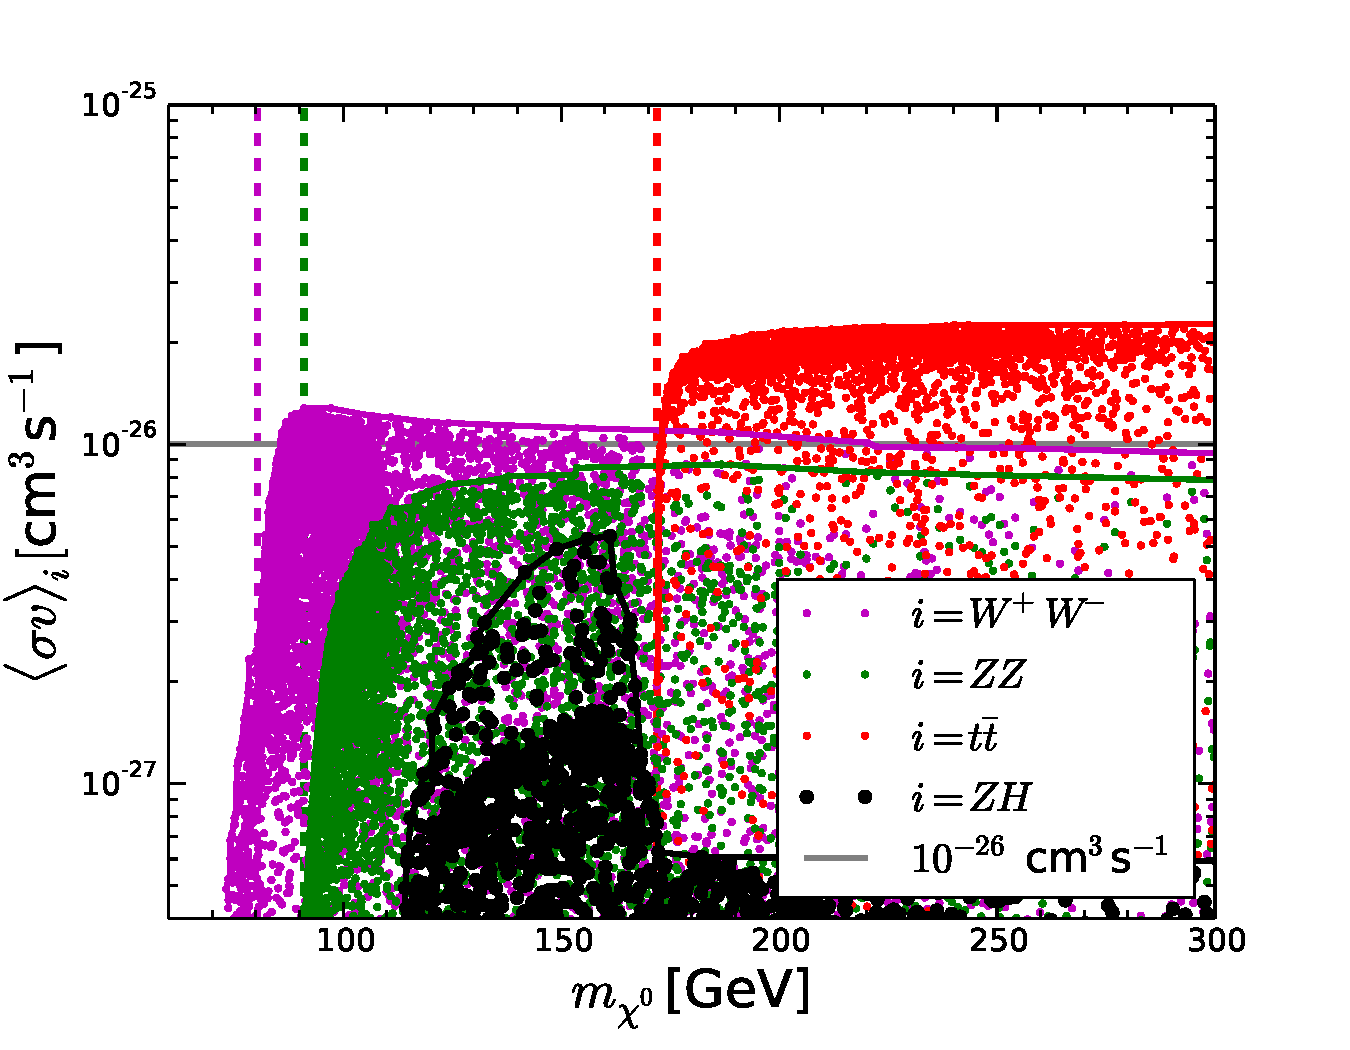
\includegraphics[scale=0.41]{GCE_MDM_vs_canales}
\end{center}
\caption{\textit{Left:} Velocity average cross-section $\langle\sigma v\rangle$, generated randomly for a big sample of the parameters of the SDFDM model (see section \ref{sec:Parameter-scan}). The green (black) line is the current constraint of indirect detection for DM annihilation into $b\bar{b}$ ($W^+W^-$) in the Dwarf spheroidal galaxies (dSph)~\cite{Ackermann:2015zua}. The gray line represent the prediction of the WIMP paradigm where the $\langle\sigma v\rangle$ reach the thermal value $10^{-26}\text{cm}^{3}\text{s}^{-1}$. \textit{Right:} Specific region where the $\langle\sigma v\rangle$ reach the the thermal value and the specific channels of DM annihilation.}
\label{fig:good-sv}
\end{figure}

Regarding direct detection, the Higgs ($Z$) exchange leads to spin independent  (spin dependent) DM nucleon scattering. From Eq. (\ref{eq:cZXX}) we get that the spin dependent (SD) cross section vanishes for $\cos2\beta=0$ or $|m_{\chi^0}|=M_D$, implying for both cases that $\tan\beta=\pm1$. In the same vein, from Eq.~(\ref{eq:cHXX}) the spin independent (SI) cross section vanishes (i.e. a blind spot as discussed by Ref.~\cite{Cheung:2013dua}) for $\sin2\beta=-m_{\chi^0}/M_D$, which leads to $m_{\chi^0}=M_N, M_D$, via Appendix~\eqref{eq:characteristic-equation}. Note that $\sigma_{SI}=0$ if $\tan\beta<0$ and that only if $M_N>M_D$ both $\sigma_{SI}$ and $\sigma_{SD}$ can be zero simultaneously. 

\section{Gamma-rays from the Galactic Center }
\label{sec:gammarays_from_the_GC}
%
The Galactic $\gamma$-ray intensity $\Phi(E_{\gamma},b,l)$ produced in self-annihilations of DM particles, where $b$ and $l$ are the Galactic latitude and longitude respectively, can be obtained from the following relation~\cite{Baltz, Bergstrom,Rott}
\begin{equation}
\Phi(E_{\gamma},b,l)= \frac{1}{2}\frac{\left\langle\sigma v \right\rangle}{4\pi m_{\chi^0}}\sum_{f} \frac{dN_{f}}{dE_{\gamma}}B_f \times J(b,l),
\label{Phi}
\end{equation}
which is the product of a term that depends solely on the inherent properties of the DM particle and an astrophysical factor $J(b,l)$ accounting for the amount of DM in the line of sight.
 The former is given in terms of the velocity-averaged annihilation cross-section $\left\langle \sigma v \right\rangle$, the differential $\gamma$-ray multiplicity per annihilation $dN_{f}/dE_{\gamma}$, the DM mass $m_{\chi^0}$ and the branching ratio $B_f$ where $f$ denotes the final state particles resulting from the annihilation. 
The astrophysical factor can be drawn as ~\cite{Bergstrom, Rott}
\begin{equation}
J(b,l)=\int^{\infty}_0 ds\; \rho\left(\sqrt{R^2_{\odot}-2sR_{\odot}\cos(b)\cos(l)+s^2}\right)^2,
\label{J}
\end{equation}
where the DM density-square is integrated along the line-of-sight $s$ and $R_{\odot}=8.25$ kpc is the distance from the solar system to the GC.

The DM halo density $\rho(r)$ is determined by N-body cosmological simulations, with recent studies preferring a generalized NFW profile~\cite{navarrofrenkwhite1997} of the form
\begin{equation}
\rho(r)=\frac{\rho_s}{\left(\frac{r}{r_s}\right)^{\gamma}\left[1+\left(\frac{r}{r_s}\right)^{\alpha}\right]^{(\beta-\gamma)/\alpha}},
\label{nfw}
\end{equation}
where we adopt the scale radius $r_s=23.1$ kpc and the parameters $\alpha=1$, $\beta=3$ as default choices.
 Recent analyses of the GCE~\cite{GordonMacias2013,Daylan:2014,CaloreCholisWeniger2015} find a best fit profile inner slope $\gamma \simeq 1.2$, corresponding to a mildly contracted DM halo.
 We normalized the density profile by fixing the local dark matter $\rho(R_\odot=8.25\; \mbox{kpc})=0.36$ GeV cm$^{-3}$.
 This was done by maximizing the likelihood of microlensing and dynamical data for the chosen profile slope (see Fig.5 of Ref.~\cite{ioccopatobertone2011}). 

The $\gamma$-ray spectra ($dN_{f}/dE_{\gamma}$) resulting from $\chi^0$ annihilations was generated with the software package \textsc{PPPC4DMID} \cite{Cirelli_cookbook}.
 We noticed that for some channels, the interpolation functions provided by this useful tool are incomplete close to the rest mass thresholds.
 In such cases, we instead generated the spectra with the Monte Carlo event generator \textsc{PYTHIA 8.1} \cite{Sjostrand:2007gs} making sure that these were in agreement with the ones in \textsc{PPPC4DMID} for higher mass ranges.
 
Because of the quadratic dependence of Eq.~\ref{Phi} on the dark matter density, the GC is expected to be the brightest DM source in the $\gamma$-ray sky. However this region also harbours many $\gamma$-ray compact objects and the Galaxy's most intense diffuse $\gamma$-ray emission produced by the interaction of cosmic rays with interstellar material. The impact of these uncertainties in the interpretation of the GCE is currently not very well understood and is the subject of many recent studies.

There are also large uncertainties associated with the predicted signal from DM self-annihilations in the GC. The DM distribution in the innermost region of our Galaxy is poorly constrained by numerical DM-only simulations and kinematic measurements of Milky Way constituents. In principle, ordinary matter is expected to affect the inner dark matter profile obtained from simulations at a certain level. The DM density could be either flattened by star burst activity that ejects baryonic material from the inner region or steepened through adiabatic contraction. Indeed, depending on the assumed DM distribution, different estimates of the expected $\gamma$-ray emission can differ by a factor of up to $\sim 50$ (see Ref.~\cite{Funk:review,Catena:2009mf}).

Dwarf spheroidal galaxies (dSph) of the Milky Way are generally thought to be much simpler targets for indirect DM detection. Although their  $J(b,l)$ factor is orders of magnitude lower than that of the GC, they contain a much cleaner $\gamma$-ray background. Reference~\cite{Ackermann:2015zua} shows that the null detection of $\gamma$-ray emission from such objects impose strong constraints on the properties of DM models. In the next sections, we will discuss the effects of these limits on the DM interpretation of the GCE. 

Here we entertain the possibility that the SDFDM model can account for the GCE while being consistent with a variety of experimental limits on DM. This is accomplished by following closely the procedure developed in Ref.~\cite{CaloreCholisWeniger2015} and expanded upon in  Ref.~\cite{Caron:2015wda,Bertoneetal}. In summary, the $\gamma$-ray fluxes obtained from our model scans are compared to the GCE data made available in Ref.~\cite{CaloreCholisWeniger2015}. In that work, the systematic and statistical uncertainties in the Galactic diffuse emission model were provided in the form of a covariance matrix $\Sigma_{ij}$, which we use here to the full extent (we refer the reader to the aforementioned article for details on the statistical formalism and the implementation of the $\chi^2$ function). As was done in Refs.~\cite{Caron:2015wda,Bertoneetal}, we modified the covariance matrix to also account for theoretical uncertainties in the $\gamma$-ray spectra generation. Namely, we rewrite $\Sigma_{ij}$ as 
\begin{equation}
\Sigma_{ij} \rightarrow \Sigma_{ij} + \delta_{ij} d^2_{i} \sigma^2_s,
\end{equation}
where $\delta_{ij}$ is the Kronecker delta, $d_i$ are the measured photon fluxes and $\sigma_s=10$\% is the adopted theoretical uncertainty~\cite{Caron:2015wda,Bertoneetal}.


For each of the SDFDM models, we calculate the corresponding $\chi^2$ (or $p$-value) and make sure that these are consistent with the null \textit{Fermi}-LAT detection of $\gamma$-rays in dSphs. As recommended in the 3FGL catalog article~\cite{Acero:2015hja}, a given source spectral model is rejected when its associated $p$-value is less than $10^{-3}$. This is the same as to say that for $24-4$ degrees of freedom ($d.o.f$), model points having a $\chi^2>45.37$ are considered bad fits to the GCE. In all relevant figures, we incorporate the 95\% upper limits on the value of $\left\langle\sigma v \right\rangle$ as extracted from Ref.~\cite{Ackermann:2015zua}.


\section{Numerical analysis}
\label{sec:Parameter-scan}

Having identified the main annihilation channels and established the procedure to calculate the $\gamma$-ray fluxes, we move to explore the regions of the parameter space that can account for the {\it Fermi} GeV excess. Namely, in this section we determine the regions that are compatible with current constraints coming from colliders, electroweak phase transition (EWPT), indirect and direct DM searches, and then assess them in light of the quality of the fit to the GCE.     

\subsection{Scan and constraints}

To this end, we scan the parameter space of our model by considering the following ranges for the model parameters:    
\begin{align}\label{eq:scan}
100<M_D/\text{GeV}<1000,&\hspace{1cm}10 <M_N/\text{GeV}<1000,\nonumber\\
10^{-4}<\lambda<10,&\hspace{1cm} 1\leq\left|\tan\beta\right|<60.
\end{align}

Essentially, we throw darts into this large space, generating several million random model points, and for each generated point we compute the DM relic density and the direct and indirect DM observables using \textsc{micrOMEGAs 4.1.8}~\cite{Belanger:2014vza} through \textsc{Feynrules 2.3}~\cite{Christensen:2008py}. Each individual model is then subjected to a large set of dark matter, precision measurement and collider constraints. In particular, we assume that the DM  relic density saturates the Planck measurement $\Omega h^2=(0.1199 \pm 0.0027)$~\cite{Ade:2013zuv} at the $3\,\sigma$ level as we are interested in considering in considering the case where this model accounts for the majority of DM. The model points are also required to be compatible with \textit{Fermi}-LAT constraints coming from dwarf spheroidal galaxies~\cite{Ackermann:2015zua}, as well as LUX~\cite{Akerib:2013tjd}, IceCube~\cite{2013PhRvL.110m1302A}, PICO-2L~\cite{Amole:2016pye} and PICO-60~\cite{Amole:2015pla}  limits for spin independent and spin dependent detection studies. 
Since the SDFM model presents new contributions to the EW precision observables (EWPO) \cite{D'Eramo:2007ga}, we impose the condition that $\Delta T < 0.2$ given that the contribution to $S$ is always negligible \cite{Calibbi:2015nha}.  Finally, the limit obtained from searches of charged vector-like particles by LEP~\cite{ALEPH:2005ab} has been taken into account by imposing the condition $M_D > 100$~GeV in Eq. (\ref{eq:scan}). 


%%%%%%%%%%%%%%%%%%%%%%%%%%%%%%%%%%%% PLOT: MD, MN, TANBETA, LAMBDA parameters
\begin{figure}[h]
\begin{center}
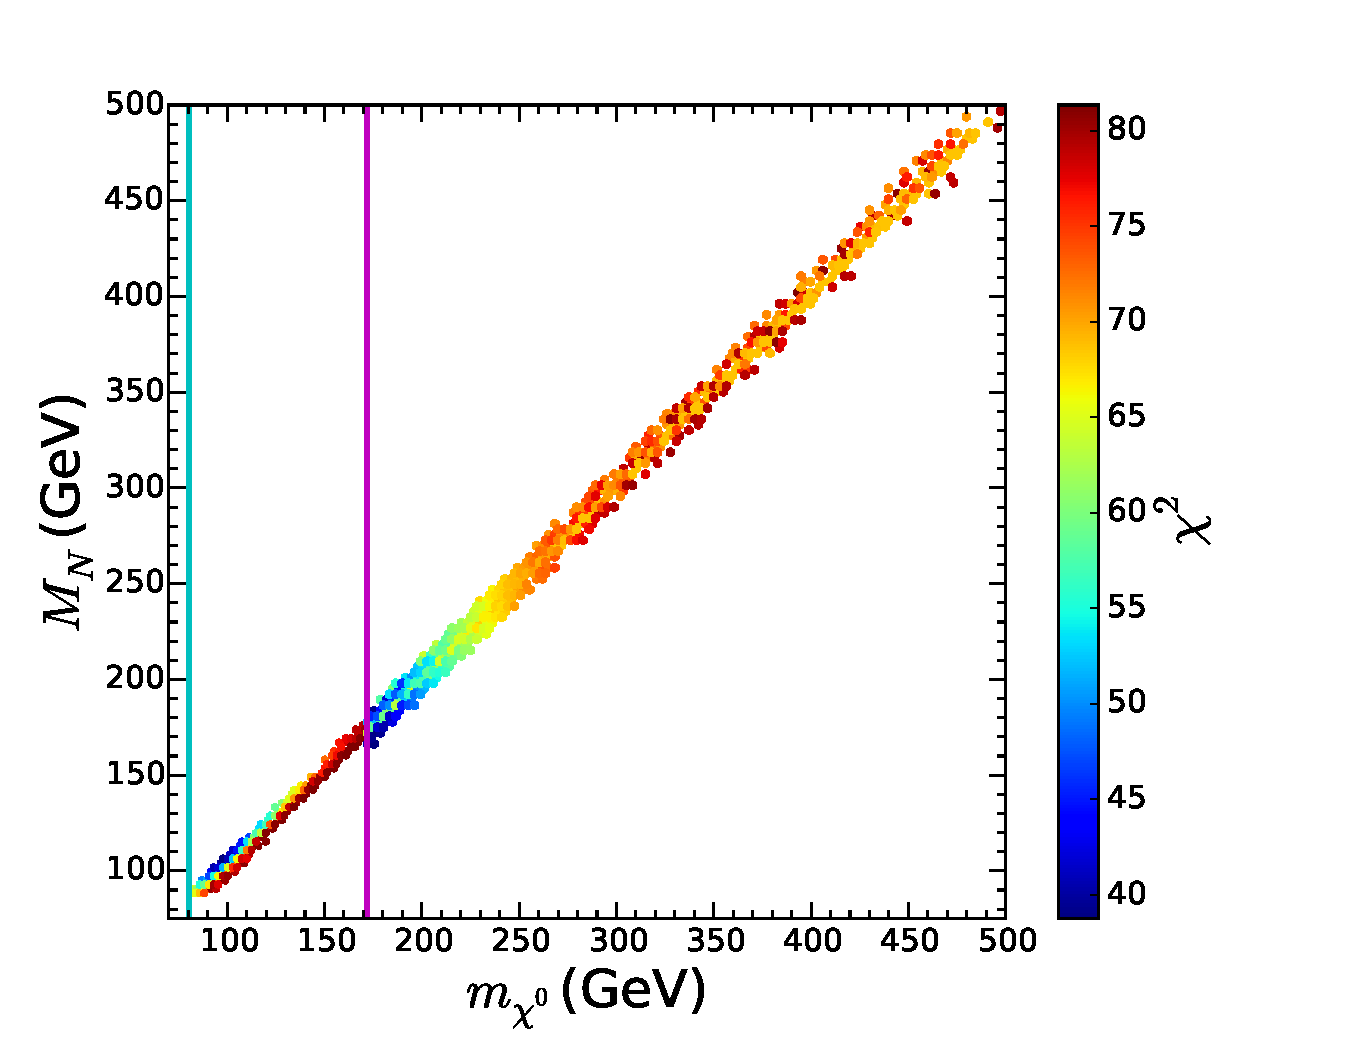
\includegraphics[scale=0.35]{GCE_MDM_vs_MN_2}  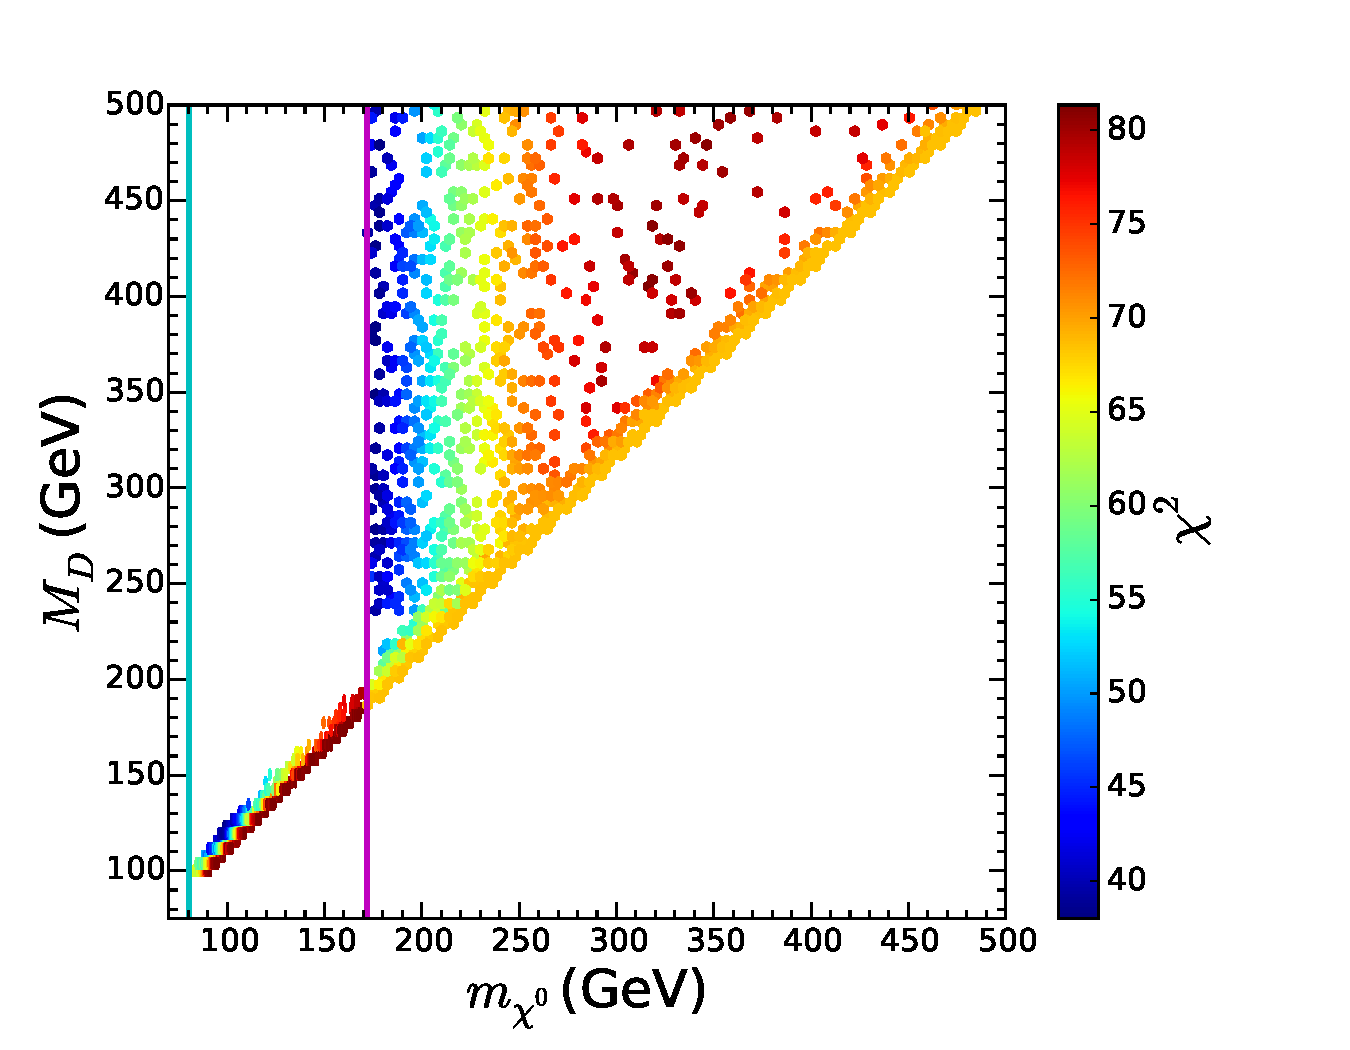
\includegraphics[scale=0.35]{GCE_MDM_vs_MD_2} 
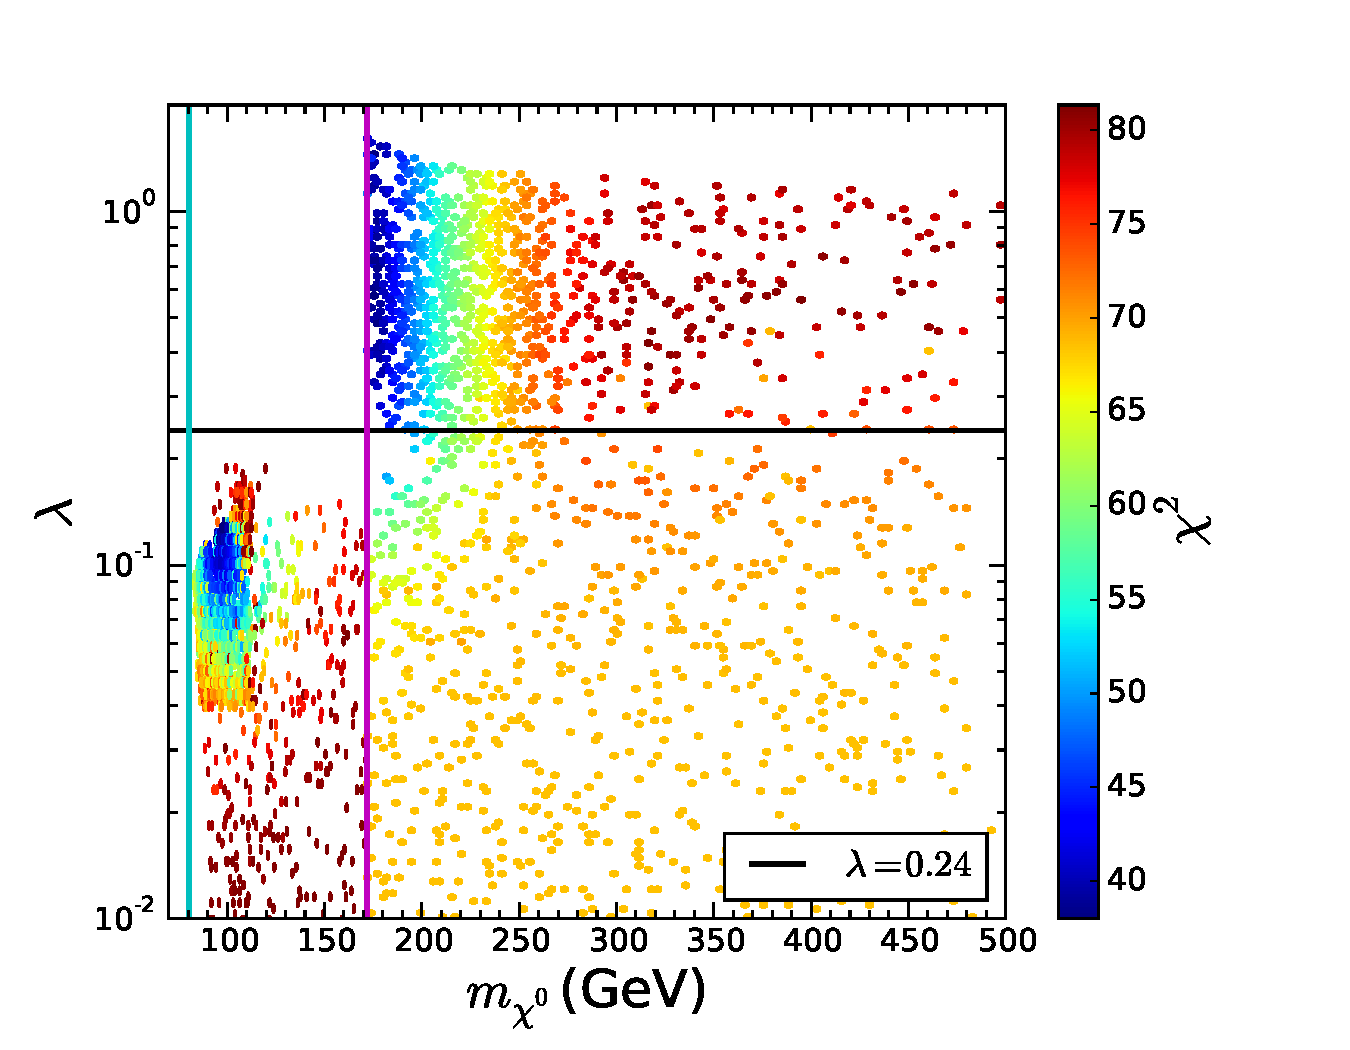
\includegraphics[scale=0.35]{GCE_MDM_vs_lambda_2}  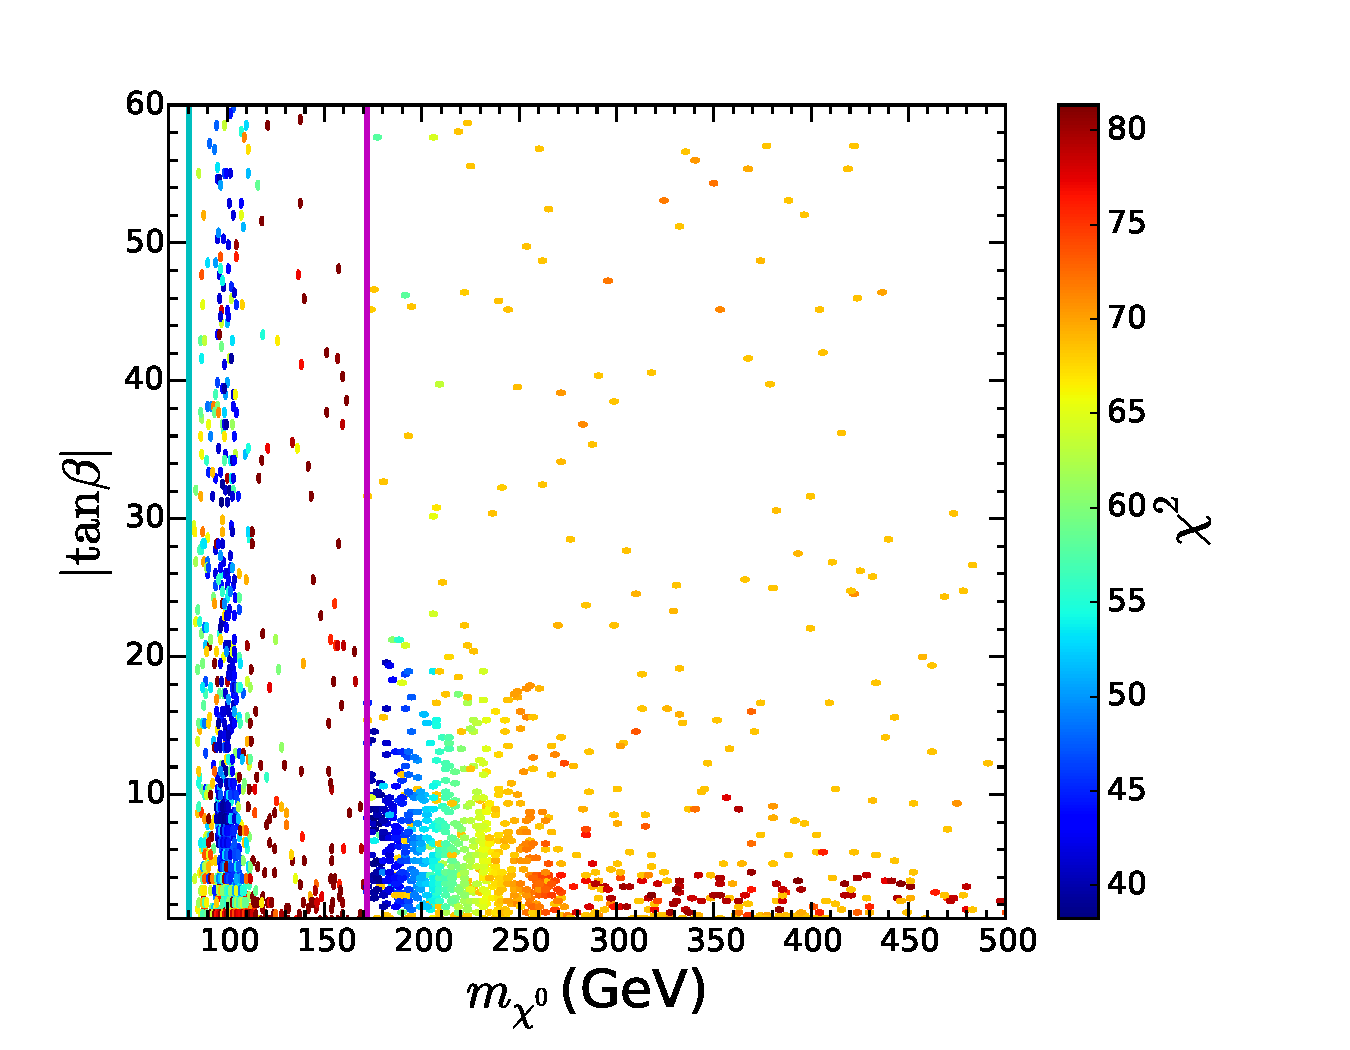
\includegraphics[scale=0.35]{GCE_MDM_vs_tanb_2}
\caption{Two-dimensional projection of the $\chi^2$ values of our fit, showing each one of the four free parameters in the SDFDM model ($M_N$, $M_D$, $\lambda$ and $|\tan \beta|$) versus the dark matter mass ($m_{\chi^0}$). 
In the bottom left panel the black line represents the supersymmetry value $\lambda\sim 0.24$, while the cyan and magenta vertical lines in all panels represent the $W$ boson mass and the top quark mass, respectively. Model points able to fit the GCE are those having a $\chi^2<45.37$ for $24-4$ d.o.f.}
\label{fig:parameters}
\end{center}
\end{figure}
%%%%%%%%%%%%%%%%%%%%%%%%%%%%%%%%%%%%%%%%%%%%%%%%%%%%%%%%%%%%%%%%%%%%%%%%%%%%%


\subsection{Results}
\label{subsec:Results}
Fig.~\ref{fig:parameters} displays the viable models in the planes ($M_N$, $m_{\chi^0}$),  ($M_D$, $m_{\chi^0}$),  ($\lambda$, $m_{\chi^0}$) and  ($|\tan\beta|$, $m_{\chi^0}$), along with the corresponding $\chi^2$ values obtained from a fit to the GCE. 
Since the fit tends to be worse for large values of $m_{\chi^0}$, we only considered DM masses  below 500 GeV. 
Furthermore, as it was discussed in Sec.~\ref{sec:modelgce}, we only studied models with $m_{\chi^0}$ above the $W$ gauge boson mass. 
It is convenient to split the results of our scan into two different regions (DM mass ranges): one in which $m_{\chi^0}$ is below the top mass (Region I) and a second one in which $m_{\chi^0}$ is larger than the mass of the top quark (Region II).  

The viable models belonging to Region I are characterized for having  $M_N\approx M_D\approx m_{\chi^0}$, that is, the DM particle is a mixture of singlet and doublet states (well-tempered DM \cite{ArkaniHamed:2006mb,Cheung:2013dua}). 
The non-observation of direct detection signals constrains the Yukawa coupling to small values ($y<0.2$). We note that this limit excludes the MSSM value $\lambda \sim 0.24$. However, $|\tan\beta|$ is not constrained to a specific value or range. 
Regarding Region II, our analysis shows that $M_N\approx m_{\chi^0}$ while $M_D\gtrsim m_{\chi^0}$. For $y\lesssim 0.3$ the DM particle should be again well tempered ($M_D\approx M_N$) whereas for larger values of $y$ we have that $M_D$ is larger than $M_N$.      
In this case the upper bound $y\lesssim 5$ comes from the Planck measurement of the DM relic density.

The viable solutions to the GCE found in Region I feature the following parameters: $M_N\sim 105$ GeV, $M_D\sim 120$ GeV, $\lambda\sim 0.12$ and $|\tan\beta|\sim 9$ which generates a DM mass of $\sim 99$ GeV with a $\chi^2$ value of $45.3$. For these parameters the dark matter annihilates mostly into $W^+W^-$. 
While for the Region II we found that the viable solutions correspond to the sample:
\begin{align}
166  < & \, M_N/\text{GeV} < \, 197 , \nonumber \\
236  < & \, M_D/\text{GeV} < \, 988 , \nonumber \\ 
0.25  < & \, \lambda < \, 1.60 ,\nonumber \\
1.87 <  &\, \tan\beta < \, 19.6,
%0.067 <  \, \tan\beta < \, 0.62,&\,\,\,\, \text{and}\,\,\,\, 1.87 <  \, \tan\beta < \, 19.6,
\end{align}
which leads to a DM mass in the range $(173-190)$ GeV with $\langle\sigma v\rangle_{t\bar{t}}/\langle\sigma v\rangle\geq 0.9$ and $\langle\sigma v\rangle_{WW}/\langle\sigma v\rangle\leq 0.1$. The fact that $\chi^0\chi^0\to t\bar{t}$ dominates, via $s$-channel exchange of a $Z$, is reflected in the required values for $y$, because it controls the coupling $c_{Z\chi^0\chi^0}$ whenever $|\tan\beta\neq1|$. 
Note also that, since $\tan\beta>0$ and $\tan\beta\neq1$, the SI and SD cross sections respectively can not be zero (no blind spot occurs). This means that the hypothesis of the SDFDM model being an explanation of the GCE can be probed in future experiments (see next section). Concerning the best $\chi^2$ obtained, we have obtained the value $38.0$ which is represented by white star in Fig.~\ref{fig:sigmav} and Fig.~\ref{fig:sigma-SI-SD}. 

Overall, the two sets of models capable of explaining GCE have DM particles $\chi^0$ with masses around $99$ GeV and $173-190$ GeV annihilating into $W^+W^-$ and $t\bar{t}$, respectively\footnote{The fact that the DM should annihilate into $W^+W^-$ and $t\bar{t}$ in order to explain the GCE is in accordance with what was stated in Ref.~\cite{Agrawal:2014oha}.}. As explained above, all of our solutions saturate the thermal relic density, making them also consistent with cosmological constraints on dark matter. 

\subsection{Probing the viable solutions with future observations}
%%%%%%%%%%%%%%%%%%%%%%%%%%%%%%%%%%%% PLOT: SIGMAV %%%%%%%%%%%%%%%%%%%%%%%%
\begin{figure}[t]
\begin{center}
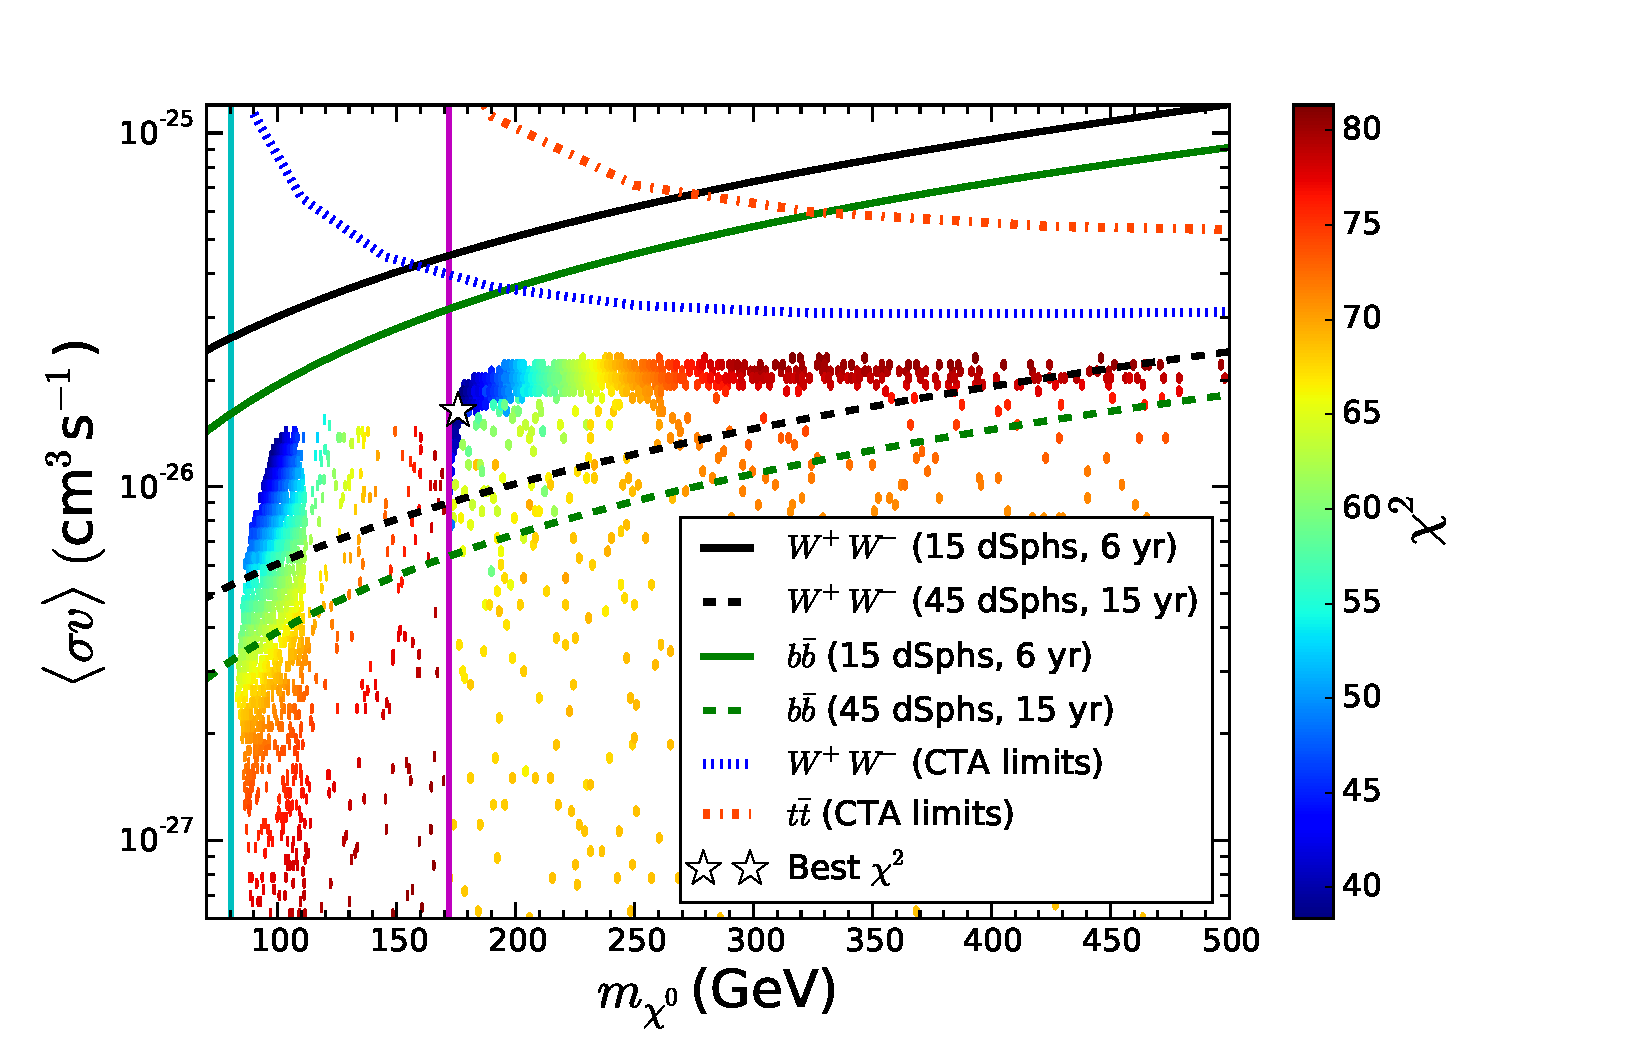
\includegraphics[scale=0.5]{GCE_MDM_vs_sigmav_3} 
\caption{The present velocity averaged annihilation cross-section as a function of the dark matter mass in comparison to current indirect detection limits in different channels. 
The 95\% C.L gamma-ray upper limits from dSphs are extracted from Ref.~\cite{Ackermann:2015zua}. The CTA limits correspond to future 100 hr of $\gamma$-rays observations of the GC and assume a generalized NFW profile with an inner slope of $\gamma=1.2$.
The star is the best-fitting model obtained from our scan. 
Vertical lines and color code are the same as in Fig.~\ref{fig:parameters}.}
\label{fig:sigmav}
\end{center}
\end{figure}
%%%%%%%%%%%%%%%%%%%%%%%%%%%%%%%%%%%%%%%%%%%%%%%%%%%%%%%%%%%%%%%%%%%%%%%%%%
The velocity averaged annihilation cross-section as a function of the dark matter mass in
comparison to current indirect detection limits in different channels along with the $\chi^2$ values found in a fit to the GCE are shown in Fig.~\ref{fig:sigmav}. 
Note that current upper limits from dSphs~\cite{Ackermann:2015zua} do not presently constrain any of the viable points. This is a consequence of the imposed requirement that models must comply with the observed DM relic density. Once this condition is applied, it generally restricts the parameter space of the SDFDM model to have a $\langle\sigma v\rangle$ less than $\sim 2\times 10^{-26}$ cm$^3$s$^{-1}$.

Future dSphs analyses with the \textit{Fermi}-LAT telescope will benefit from larger statistics and potential discoveries of new ultra-faint dwarfs. At low energies the point spread function (PSF) sensitivity for the LAT instrument increases approximately as the square-root of the observation time, while at high energies, the PSF increases roughly linearly with time. The $\gamma$-ray bounds reported in Ref.~\cite{Ackermann:2015zua} used 6 years of \textsc{Pass8} \textit{Fermi} data taken from 15 dwarf spheroidals. Thus, we can conservatively estimate that with 15 years of \textit{Fermi} data and 3 times more dSphs discovered (45 dSphs) in the next few years, the LAT constraints will improve by a factor of $(\sqrt{15}/\sqrt{6})\times 3 \simeq 5$ compared to the current ones. 

As can be seen in Fig.~\ref{fig:sigmav}, the 15 years \textit{Fermi}-LAT forecast in the $W^{+}W^{-}$ channel indicates that future dSphs observations will be in significant tension with the set of favoured models found in Region I. Although the \textit{Fermi} collaboration have not yet released equivalent limits for $t\bar{t}$ final states, these should be comparable at the percentage level~\cite{Cirelli_cookbook} with those in the $b\bar{b}$ channel. We thus use the latest limits accordingly, and show that \textit{Fermi}-LAT dwarfs will also have the ability to test our $t\bar{t}$ solution (Region II). However, here an important remark is in order. As discussed in Ref.~\cite{Caloreetal:Taleoftails}, astrophysical uncertainties in the DM parameters can affect the expected $\gamma$-ray emission in a manner that makes the annihilation cross-section uncertain by a factor of $\sim 5$ up and down. Hence, both of our solutions could in principle still escape future \textit{Fermi}-LAT dwarfs limits if astrophysical uncertainties are taken into consideration. Also, as there is likely to be at least some millisecond pulsar contribution, the actual $\langle\sigma v\rangle$ could be correspondingly lower and so even harder to detect.     

Using the method presented in Ref.~\cite{Silverwood:2014yza}, we compute the 95\% confidence level upper limits on the annihilation cross section that will be achievable with the upcoming ground-based $\gamma$-ray observatory CTA~\cite{2011ExA....32..193A}, assuming annihilation into $W^+W^-$ and $t\bar{t}$ channels and the halo model described earlier in this paper. These limits use the 28 spatial bin morphological analysis, and include a systematic uncertainty of 1\% and the effects of the galactic diffuse emission. We find the 95\% confidence level upper limits by first calculating the best fit annihilation cross section, and then correctly increasing the cross section until $-2 \ln \mathcal{L}$ increases by 2.71 whilst profiling over the remaining signal model parameters. These limits are shown in Figure~\ref{fig:sigmav}, and show that observations towards the GC by CTA will be unable to confirm or exclude the SDFDM model as an explanation of the GCE. 

%
%%%%%%%%%%%%%%%%%%%%%%%%%%%%%%%%%%%% PLOT: SI , SD  %%%%%%%%%%%
\begin{figure}[t]
\begin{center}
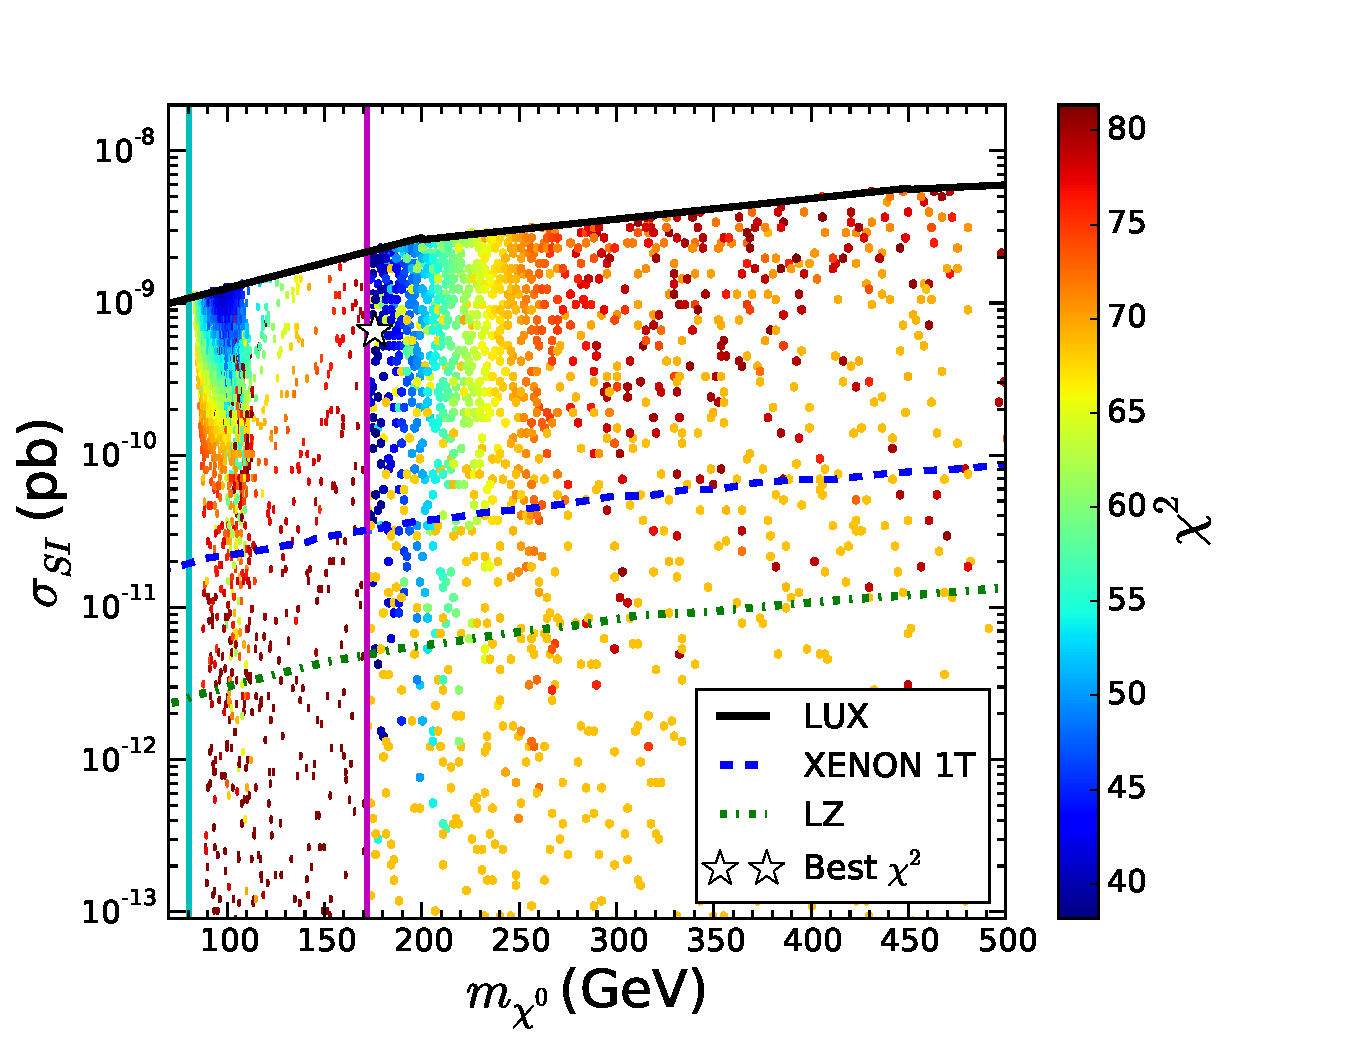
\includegraphics[scale=0.39]{GCE_MDM_vs_sigmaSI_5}  
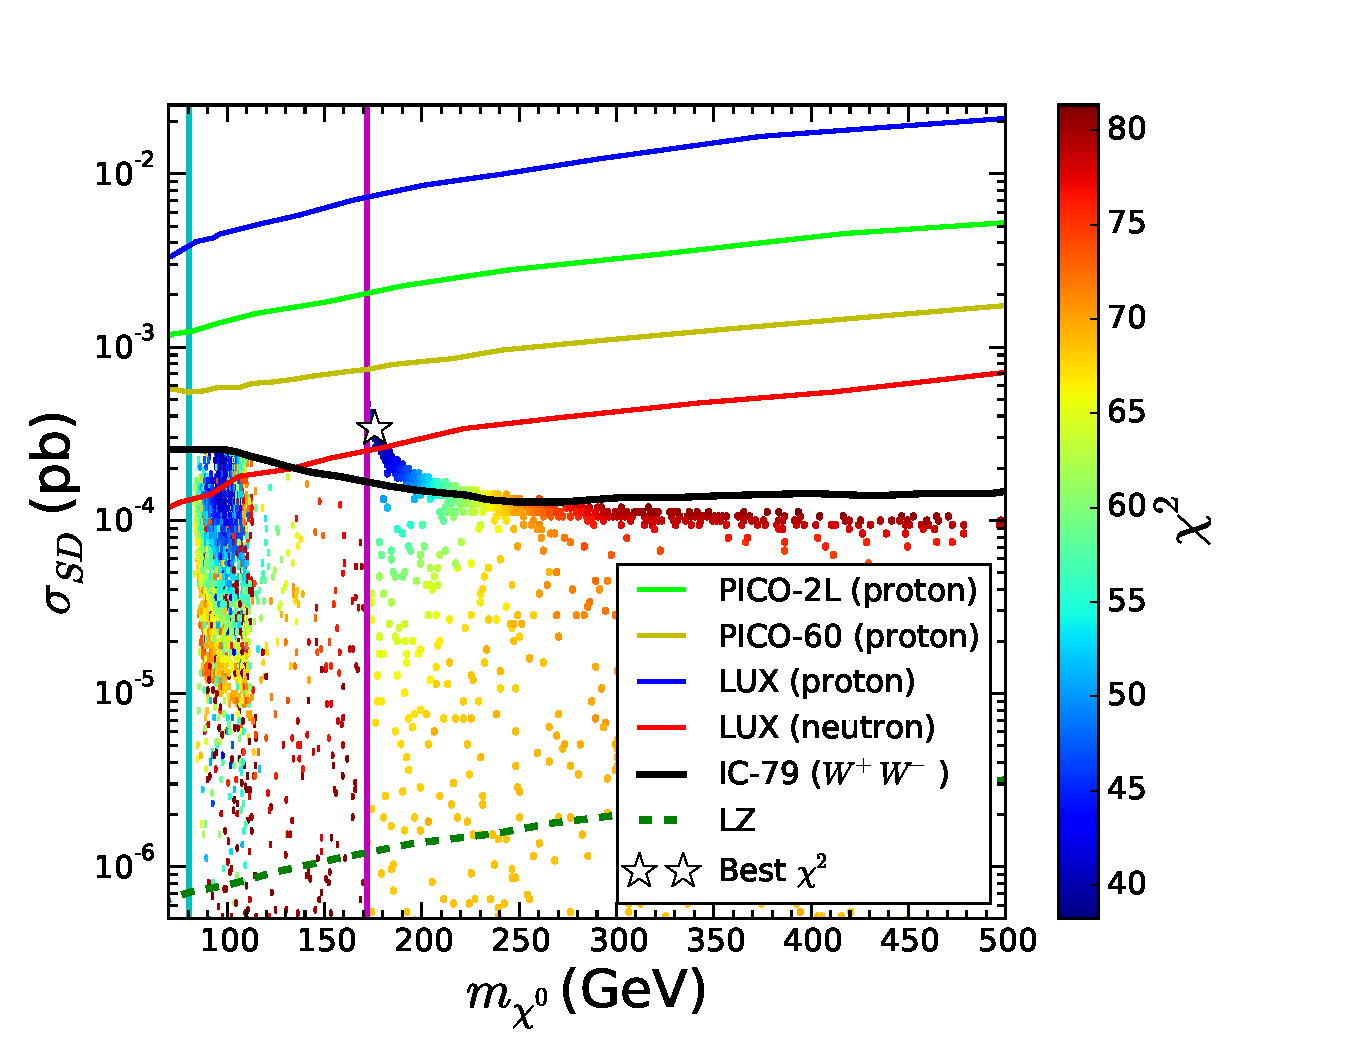
\includegraphics[scale=0.39]{GCE_MDM_vs_sigmaSD_5} 
\caption{Spin-independent $\sigma_{SI}$ (left) and spin-dependent $\sigma_{SD}$ (right) direct detection cross sections in the SDFDM model in comparison to current and future direct detection limits. 
The left panel displays current limits from the LUX experiment (black solid line) and the expected limits from the forthcoming XENON-1T and LZ~\cite{Cushman:2013zza} experiments (blue dashed and green dot-dashed lines).
The right panel shows the IceCube limits in the $W^+W^-$ channel (black solid line) from null observations of the sun,  the PICO-2L~\cite{Amole:2016pye} (green light solid line) and PICO-60~\cite{Amole:2015pla} (yellow solid line) limits as well as the LZ sensitivity (green dashed line). The most recent constraints from LUX~\cite{Akerib:2016lao} (red and blue solid lines) are also overlaid. 
The star is the best-fitting model obtained from our scan. 
Vertical lines and color code are the same as in Fig.~\ref{fig:parameters}.
}
\label{fig:sigma-SI-SD}
\end{center}
\end{figure}
%%%%%%%%%%%%%%%%%%%%%%%%%%%%%%%%%%%%%%%%%%%%%%%%%%%%%%%%%%%%%%%
%
The SDFDM model can also be tested through direct dark matter detection searches. This results from either the spin-independent (SI) or spin-dependent (SD) scattering of the $\chi^0$ particle off a target nucleus. Fig.~\ref{fig:sigma-SI-SD} displays the predicted SI and SD cross sections for our model set together with several present and anticipated experimental constraints. Namely, we overlaid the upper limits from the LUX experiment, and the expected limits from XENON-1T and LZ~\cite{Cushman:2013zza}. As can be seen, these future experiments, in particular LZ, will be able to cut deeply into the model set and confirm or rule out the DM explanation of the GCE if it is the only extended source emitting high energy photons in the GC. We also note that available constrains from IceCube are just on the edge of probing the set of models that could account for the excess. In fact, the most recent limits on the spin-dependent WIMP-nucleon elastic cross-section from LUX~\cite{Akerib:2016lao} have begun to disfavour the best fit region. This is per se, a great example of the importance of a combined effort of different search techniques in the quest for dark matter.    
 

%\section{Conclusions}
%\label{sec:conclusions}
%
%In this work we have entertained the possibility of finding model points in the SDFDM model that can explain the GCE while being in agreement with a multitude of different direct and indirect DM detection constrains. We found two viable regions: (i) DM particles present in the model with masses of $\sim 99$ GeV annihilating mainly into $W$ bosons with branching ratios greater than $\sim 70\%$, (ii) and a second region where the DM particle mass is in the range $\sim (173-190)$ GeV annihilating predominantly into the $t\bar{t}$ channel with branching ratios greater than $\sim 90\%$. Our analysis assumed that the DM is made entirely out of the lightest stable particle $\chi^0$ of the SDFDM model. Despite this being a very restrictive assumption, we have demonstrated that there exist models capable of accounting for the GeV excess in the GC that can be fully tested by the forthcoming XENON-1T and LZ experiments as well as by future \textit{Fermi}-LAT observations in dwarf galaxies. Interestingly, the most recent limits presented by LUX are able to probe a fraction of the good fitting models to the GCE found in this work. We also showed through realistic calculations of CTA performance when observing the GC that this instrument will not have the ability to confirm the SDFDM model if it is causing the GCE.

         



%
%\chapter{Gamma rays lines in the SDFDM model with real scalars singlets}
%\label{sec:gammarays-SDFDM}
%
After the freeze-out of the Dark Matter (DM) in the early Universe, the annihilation continuous to today but in smaller rate, principally in regions where the concentration of DM is high, like the center of our Galaxy.
Therefore, exits the possibility to see this annihilations looking for in the flux that reach the earth and in that way check the freeze-out mechanism. However to measure the expected flux after DM annihilation is so challenging because It is typically much smaller than the background flux generated for Astrophysical processes.

One strategy to identify DM signals is to search for gamma ray spectral features as gamma ray lines.
In the case of the Milky Way center, DM particles are expected to be very non-relativistic, $v\approx 10^{-3}$, thus generating monoenergety photons in the annihilation process. They are qualitatively very different from the ones expected from the known astrophysical background and for that reason a good form to find the DM in the Universe.
Search for gamma ray spectral features provide limits on the model parameter space and sometimes are competitive with direct detection.  

In the particular case of the SDFDM model with real scalars singlets we can have scalar or fermionic DM like we described in the Sec.~\ref{sec:model-with-scalars}. The goal of this chapter is to describe the spectral features generated in this two cases.





%%%%%%%%%%%%%%%%%%%%%%%%%%%%%%%%%%%%%%%%%%%%%%%%%%%%%%%%%%%%%%%%%%%%%%%%%%%%%%%%%%%%%%%%%%%%%%%%%
\section{DM annihilation into $\gamma\gamma$ and $\gamma Z$}

\subsection{Four-momentum for DM annihilation into $\gamma\gamma$ and $\gamma Z$}

\begin{figure}[h]
\begin{center}
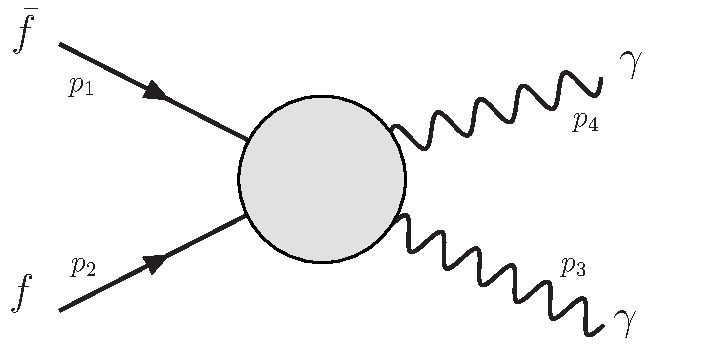
\includegraphics[scale=0.45]{annihilation_in_gammagamma}
\end{center}
\caption{General annihilation into two photons.}
\label{fig:annihilationgg}
\end{figure}

In the s-wave approximation we consider an initial state of two particles (fermions or scalars) non-relativistic with a initial relative velocity going to zero. In this case, we have an initial state with orbital angular momentum $L=0$ and spin $S=0$. The momentum shown in the Fig.~\eqref{fig:annihilationgg} for the case of fermions annihilation process in the CM frame are approximately given by
\begin{align}
p_{1}=&(E,m\vec{v})\approx(m,0,0,0)\nonumber\\
p_{2}=&(E,-m\vec{v})\approx(m,0,0,0)\nonumber\\
p_{3}=&(E_{\gamma},0,0,E_{\gamma})\nonumber\\
p_{4}=&(E_{\gamma},0,0,-E_{\gamma})\,.
\end{align}
%
Therefore, in this limit, the Mandelstan variables are
\begin{align*}
s=&(p_1+p_2)^2=4E^2=4m^2(1+v^2)=4m^2\left(1+\dfrac{v_r^2}{4}\right)=4m^2(1+\epsilon)\\
t=&(p_1-p_3)^2=p_1^2+p_3^2-2p_1p_3\approx m^2-2mE_{\gamma}\\
u=&(p_1-p_4)^2=p_1^2+p_4^2-2p_1p_4\approx m^2-2mE_{\gamma}\,,
\end{align*}
where $v_r=\sqrt{4\epsilon}$ is the relative velocity of the two initial particles in the CM frame.
Now, using the known relation $s+t+u=\sum_im_i^2=2m^2$ and the last equation, we get that $E_{\gamma}\approx m$ and therefore we get the next approximate relation for the Mandelstan variables
\begin{align}
u&\rightarrow t \nonumber\\
t&\rightarrow m^2-\dfrac{s}{2} \nonumber\\
s&\rightarrow 4m^2(1+\epsilon)\,,
\end{align}
where $\epsilon\approx 0$ take into account the non-zero initial velocity of the particles.



\begin{figure}[h]
\begin{center}
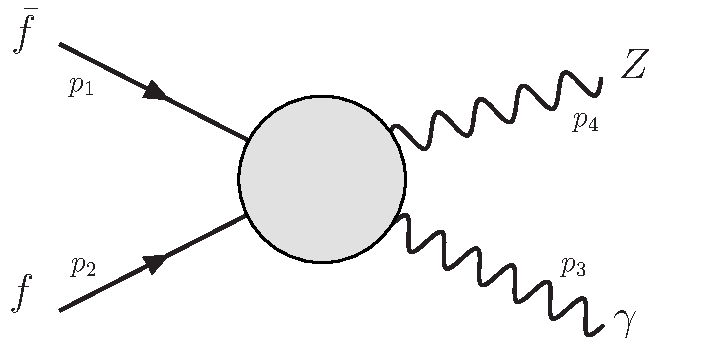
\includegraphics[scale=0.45]{annihilation_in_gammaz}
\end{center}
\caption{General annihilation into one photon and one Z gauge boson.}
\label{fig:annhilation-gz}
\end{figure}
%
In this case of DM annihilation into $\gamma Z$, the momentums shown in the Fig.~\eqref{fig:annhilation-gz} in the s-wave limit are
\begin{align}
p_1=&(E,m\vec{v})\approx(m,0,0,0)\nonumber\\
p_2=&(E,-m\vec{v})\approx(m,0,0,0)\nonumber\\
p_3=&(E_{\gamma},0,0,E_{\gamma})\nonumber\\
p_4=&(E_{Z},0,0,-|\vec{p}_{Z}|=-E_{\gamma})\,.
\end{align}
Using the conservation of the energy and the momentum we have
\begin{align}
E_{\gamma}=&m-\dfrac{m_{Z}^2}{4m}\nonumber\\
E_{Z}=&2m-E_{\gamma}\,.
\end{align}
%
The Mandelstan variables for this process are
\begin{align}
s=&(p_1+p_2)^2=p_1^2+p_2^2+2p_1p_2 = 4m^2(1+\epsilon)\nonumber\\
t=&(p_1-p_3)^2=p_1^2+p_3^2-2p_1p_3\approx m^2-2mE_{\gamma}=-m^2+\dfrac{m_Z^2}{2}\nonumber\\
u=&(p_1-p_4)^2=p_1^2+p_4^2-2p_1p_4\approx m^2+m_{Z}^2-2mE_{Z}=-m^2+\dfrac{m_Z^2}{2}\,.
\end{align}
%
Thus, using the equation $s+t+u=\sum_im_i^2=2m^2+m_Z^2$, we get the next relation 
\begin{align}
u&\rightarrow t \nonumber\\
t&\rightarrow m^2+\dfrac{m_Z^2}{2}-\dfrac{s}{2} \nonumber\\
s&\rightarrow 4m^2(1+\epsilon)\,,
\end{align}
where $\epsilon\approx 0$ take into account the non-zero initial velocity of the particles.







%%%%%%%%%%%%%%%%%%%%%%%%%%%%%%%%%%%%%%%%%%%%%%%%%%%%%%%%%%%%%%%%%%%%%%%%%%%%%%%%%%%%%%%%%%%%%%%%%%%%%%%%%%%%
\section{Gamma-ray lines spectral features from scalar DM}

\begin{figure}
\centering
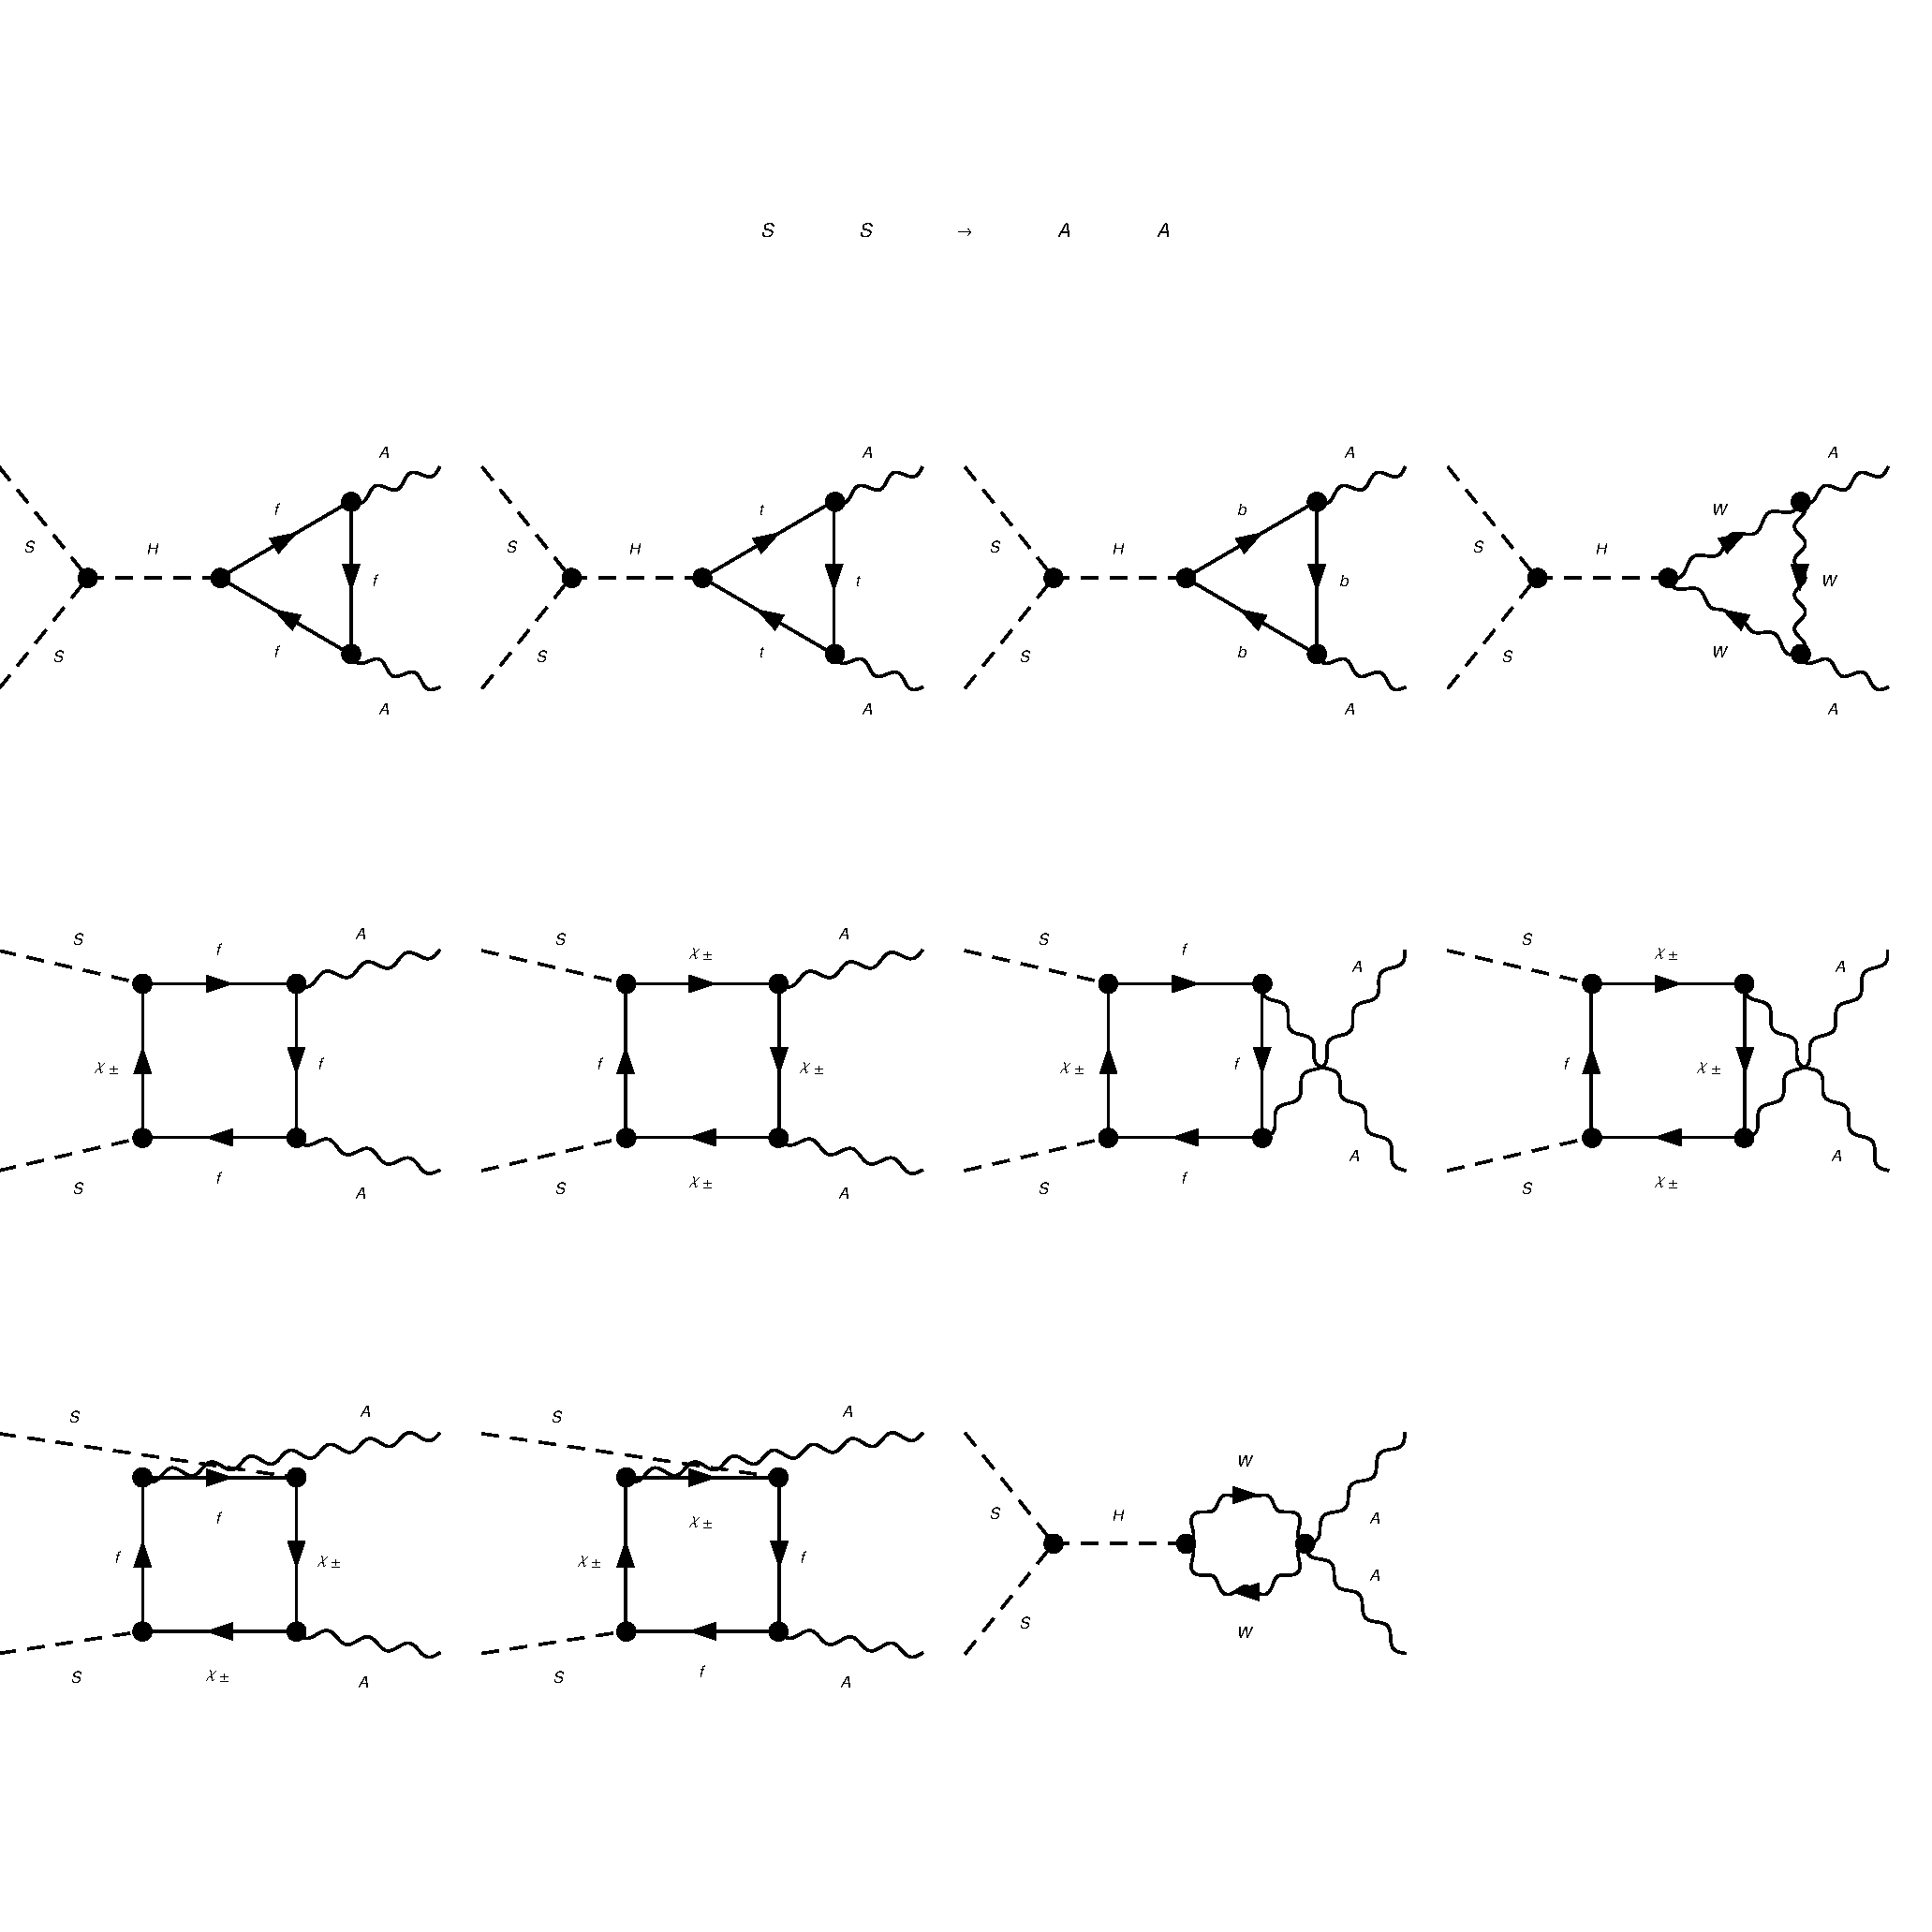
\includegraphics[scale=0.52]{T13A-scalar-to-GG-diagrams}
\caption{Feynman diagrams for $S S \to\gamma\gamma$ generated with \textsc{FeynArts}~\cite{Hahn:2000kx}. The diagrams generating the annihilation into $\gamma Z$ can be obtained by replacing one $\gamma$ in the final state by a Z-boson. In order to be more readable we show the diagrams in the unitary gauge. We only used the third family of quarks and one lepton family $f$.  We don't show the equivalent topologies with crossed initial or final state legs.}
\label{fig:scalar-to-GG}
\end{figure}

In general, the DM annihilation into $\gamma\gamma$ and $\gamma Z$ are processes generated at one loop level. They are so complicated and we have to use some computational tools that we will describe latter and use some analytical fats as the gauge and the $CP$ symmetry invariance.

In general, we used the Feynman gauge which is mandatory for the implementation in \textsc{FormCalc}~\cite{Hahn:1998yk} via \textsc{FeynRules}~\cite{Christensen:2008py}. In the Fig.~\ref{fig:scalar-to-GG} we show the Feynman diagrams for DM annihilation into $\gamma\gamma$ generated with \textsc{FeynArts}~\cite{Hahn:2000kx}. The diagrams for the annihilation into $\gamma Z$ are the same. They can be obtained by replacing one photon in the final state by the Z boson. In order to be more readable we show the diagrams in the unitary gauge. We only used the third family of quarks and one lepton family $f$.  We don't show the equivalent topologies with crossed initial or final state legs.

\subsection{Amplitude for scalar DM annihilation}

In general, it can be shown that the amplitude for scalar DM annihilation into $\gamma\gamma$ can be cast as
%
\begin{align}
\mathcal{M_{\gamma\gamma}}=&(\mathcal{M_{\gamma\gamma}})^{\mu\nu}\epsilon_{\mu}^*(p_3)\epsilon_{\nu}^*(p_4)
=\mathcal{A}_{\gamma\gamma}\left(g^{\mu\nu}-\dfrac{p_4^{\mu}p_3^{\nu}}{2m^2}\right)\epsilon_{\mu}^*(p_3)\epsilon_{\nu}^*(p_4)\,,
\end{align} 
%
where, $\mathcal{A}_{\gamma\gamma}$ is an scalar function (form factor), $\epsilon^*(p_3)_{\mu}$ and $\epsilon^*(p_4)_{\nu}$ are the polarization vectors of the photons and $m$ is the DM mass. Note that $\mathcal{M}^{\mu\nu}$ satisfied the Ward identity
$p_{3\mu}\mathcal{M}^{\mu\nu}=p_{4\nu}\mathcal{M}^{\mu\nu}=0\,$.
Even more, in the limit of zero relative velocity it can be shown that
%
\begin{align}
\label{eq:M-scalar-GG}
\mathcal{M_{\gamma\gamma}}=\mathcal{A}_{\gamma\gamma}\,g^{\mu\nu}\epsilon_{\mu}^*(p_3)\epsilon_{\nu}^*(p_4)\,.
\end{align}

On the other hand, the amplitude for annihilation into $\gamma Z$ can be cast, in the zero velocity limit, as
\begin{align}
\label{eq:M-scalar-GZ}
\mathcal{M}_{\gamma Z}=\mathcal{A}_{\gamma Z}\,g^{\mu\nu}\epsilon_{\mu}^*(p_3)\epsilon_{\nu}^*(p_4)\,,
\end{align} 
%
where $\mathcal{A}_{\gamma Z}$ is the corresponding form factor. 
As you can see, it is almost equal to the Eq.~\eqref{eq:M-scalar-GG} with the corresponding form factor. 


Now, we use the programs \textsc{FeynArts}~\cite{Hahn:2000kx} and \textsc{FormCalc}~\cite{Hahn:1998yk} to compute the amplitudes $\mathcal{M}_{\gamma\gamma}$ and $\mathcal{M}_{\gamma Z}$. In general, when \textsc{FeynArts} and \textsc{FormCalc} compute the amplitude we get an big expression that in general depend of the Passarino Veltman one loop integrals that we describe in the Appendix~\ref{sec:passarino-veltman}. Numerically we can evaluated this expression using \textsc{LoopTools}~\cite{Hahn:1998yk}. However, our goal is to get an analytical result and for that reason we implement an algorithm that we describe in the Appendix~\ref{sec:CD-reduction} in order to reduce the Passarino Veltman integrals in the \textsc{FormCalc} output. The algorithm reduce the fourth-point function to three point functions and all the coefficients tensor of the loop integrals. Usually, the results are given in terms of the scalar Passarino Veltman $C_0$ which can be given in terms of the dilogarithm Li$_{2}$ functions. In this case, the notation is more compact and readable.

The form factor obtained are:
\begin{align}
\label{eq:form-factor-SSGG}
\mathcal{A}_{\gamma\gamma}=\mathcal{A}^{h_i}_{\gamma\gamma} + \mathcal{A}^{\lambda_{SH}}_{\gamma\gamma}
\end{align}
%
\begin{align}
\mathcal{A}^{h_i}_{\gamma\gamma}
=&-\dfrac{\alpha\, h_{i}^2}{\pi} \Bigg{\{ } 2+m^2 \Big{[}
 \dfrac{1-\mu+\epsilon}{1+\mu-\epsilon}\dfrac{2\epsilon}{\mu-\epsilon}C_0(-m^2,m^2,0;m_{fi}^2,M_D^2,m_{fi}^2)\nonumber \\
+&\dfrac{1-\mu-\epsilon}{1-\mu+\epsilon}\dfrac{2\mu}{\epsilon-\mu}C_0(-m^2,m^2,0;M_D^2,m_{fi}^2,M_D^2)
+\dfrac{4\epsilon(1-\epsilon)}{1+\mu-\epsilon}C_0(4m^2,0,0;m_{fi}^2,m_{fi}^2,m_{fi}^2)\nonumber \\
+&\dfrac{4\mu(1-\mu)}{1+\epsilon-\mu}C_0(4m^2,0,0;M_D^2,M_D^2,M_D^2) \Big{] } \Bigg{\} } 
\end{align}
%

\begin{align}
\mathcal{A}^{\lambda_{SH}}_{\gamma\gamma}
=&\dfrac{\alpha}{\pi}\lambda^{SH} \bigg(\dfrac{12 m^2 + 3 m_h^2 + 16 m_t^2 + 18 m_W^2}{3(4 m^2 -  m_h^2)} +\dfrac{32 (m^2 - m_t^2) m_t^2}{3 (-4 m^2 + m_h^2)}C_0(4m^2,0,0;m_t^2,m_t^2,m_t^2)\\
&+\dfrac{m_W^2 (-24 m^2 + m_h^2 + 12 m_W^2)}{(4 m^2 - m_h^2)}C_0(4m^2,0,0;m_W^2,m_W^2,m_W^2) \bigg)\,,
\end{align}
%
where $\epsilon = m_{fi}^2/m^2$ and $\mu = M_D^2/m^2$.
$C_0$ is the scalar three-point Passarino-Veltman integral~\cite{Passarino:1978jh}. \\
Note that wee split the amplitude in two gauge invariant parts; $\mathcal{A}^{h_i}_{\gamma\gamma}$ which only depend of the coupling $h_{i}$ of the Lagrangian~\eqref{eq:lt13a} and generated the boxes diagrams shown in the Fig.~\ref{fig:scalar-to-GG}. This amplitude were computed and analyzed in~\cite{Ibarra:2014qma}, for that reason we didn't do an detailed analysis of this case, it only help us to check that our algorithm of the loop integrals is working properly. 
The other contribution $\mathcal{A}^{\lambda_{SH}}_{\gamma\gamma}$ seems to be less important because $\lambda^{SH}$ needs to be small~\cite{Ibarra:2014qma} according to direct detection's experiments (LUX and XENON1T).


%\begin{widetext}
\begin{eqnarray}
\label{eq:form-factor-SSGZ}
\mathcal{A}_{\gamma Z}\!\!&\,=\,&\!\!
-\dfrac{\alpha\, h_{i}^2 \tan\theta_W}{\pi} \Bigg{\{ } 
2-\frac{\xi}{4-\xi}B_0\left(m_Z^2;m_{fi}^2,m_{fi}^2\right)
-\frac{\xi}{4-\xi}B_0\left(m_Z^2;M_D^2,M_D^2\right)\nonumber\\
&&
+\frac{2\xi\left(1+\mu+\epsilon\right)}
{\left(4-\xi\right)\left(1+\mu-\epsilon\right)\left(1+\epsilon-\mu\right)}
\left[1-\frac{1-\mu+\epsilon}{1+\mu+\epsilon}\frac{\epsilon}{2}\right]
B_0\left(m^2;m_{fi}^2,M_D^2\right)\nonumber\\
&&
-\frac{\epsilon}{1+\mu-\epsilon}\frac{\xi}{4-\xi}
B_0\left(4m^2;m_{fi}^2,m_{fi}^2\right)
-\frac{2\mu}{1+\epsilon-\mu}\frac{\xi}{4-\xi}
B_0\left(4m^2;M_D^2,M_D^2\right)\nonumber\\
&&
+m_\chi^2\left\{
\frac{\epsilon}{2}\frac{4-4\epsilon-\xi}{1+\mu-\epsilon}
C_0\left(m_Z^2,4m^2,0;m_{fi}^2,m_{fi}^2,m_{fi}^2\right)
+\mu\frac{4-4\mu-\xi}{1+\epsilon-\mu}
C_0\left(m_Z^2,4m^2,0;M_D^2,M_D^2,M_D^2\right)\right.\nonumber\\
&&
+\frac{\epsilon}{2}\left[\frac{\left(4+\xi\right)\left(-2+2\mu+2\epsilon+\xi\right)}
{\left(1+\mu-\epsilon\right)\left(4\epsilon-4\mu+\xi\right)}
+\frac{1}{2}\frac{4-4\epsilon-\xi}{1+\mu-\epsilon}
\right]
C_0\left(-m^2+\frac{m_Z^2}{2},m^2,0;m_{fi}^2,M_D^2,m_f^2\right)\nonumber\\
&&
+\frac{\mu}{2}\left[\frac{\left(4+\xi\right)\left(-2+2\epsilon+2\mu+\xi\right)}
{\left(1+\epsilon-\mu\right)\left(4\mu-4\epsilon+\xi\right)}
-\frac{8\epsilon}{4\mu-4\epsilon+\xi}
\right]
C_0\left(-m^2+\frac{m_Z^2}{2},m^2,0;M_D^2,m_{fi}^2,M_D^2\right)\nonumber\\
&&
+\left[
\frac{2\xi\left(1+\mu\right)+\epsilon\left(4\mu-\xi\right)}{4\left(1+\mu-\epsilon\right)}
-\frac{4\left(1+\mu\right)}{4-\xi}+\frac{4\mu\left(1+\mu-2\epsilon\right)}{4\mu-4\epsilon+\xi}
\right]C_0\left(-m^2+\frac{m_Z^2}{2},m^2,m_Z^2;m_{fi}^2,M_D^2,m_{fi}^2\right)\nonumber\\
&&
+\left[
\frac{2\mu\left(1-\mu+3\epsilon\right)+\xi\left(1+\epsilon\right)}
{2\left(1+\epsilon-\mu\right)}
-\frac{4\left(1+\mu+\epsilon\right)}{4-\xi}
+\frac{4\epsilon\left(1+3\mu+\epsilon\right)}{4\epsilon-4\mu+\xi} \right]\nonumber \\
&&
\left. C_0\left(-m^2+\frac{m_Z^2}{2},m^2,m_Z^2;M_D^2,m_{fi}^2,M_D^2\right)
\right\} \Bigg{\} } \,,
\end{eqnarray}
%\end{widetext}
where $\xi=m_Z^2/m^2$ and $B_0$ is the Passarino Veltaman two-point function defined in the Appendix~\ref{sec:passarino-veltman}.
%\begin{equation}
%B_0\left(p_1^2;m_1^2,m_2^2\right)=
%\int\frac{d^d\ell}{i\pi^2}
%\frac{1}{\ell^2-m_1^2}\frac{1}{\left(\ell+p_1\right)^2-m_2^2}\,.
%\end{equation}



%%%%%%%%%%%%%%%%%%%%%%%%%%%%%%%%%%%%%%%%%%%%%%%%%%%%%%%%%%%%%%%%%%%%%%%%%%%%%%%%%%%%%%%%%%%%%%%%%%%%%
\subsection{Velocity averaged annihilation cross section $\langle \sigma v \rangle$ for scalar DM annihilation into $\gamma\gamma$ and $\gamma Z$}

In the the Appendix~\ref{sec:sigmav} we compute the thermal velocity averaged annihilation cross section for each process.
For the case of DM annihilation into two photons~Fig.\ref{fig:annihilationgg}, $\chi^0\chi^0\rightarrow\gamma\gamma$: $m_1=m_2=m$, $m_3=m_4=0$, it is given by
%
\begin{align}
\langle\sigma v_r\rangle=&\dfrac{1}{32\pi\, m^2}\overline{{|\mathcal{M}_{\gamma\gamma}|^2}}\left(1-\dfrac{v_r^2}{8}+\mathcal{O}(v_r^4)\right)\,.
\end{align}
Thus, using the Eq.~\eqref{eq:M-scalar-GG}, the s-wave contribution is
\begin{align}
\langle\sigma v_r\rangle\Big{\vert}_{\text{s-wave}}
=&\dfrac{1}{32\pi\, m^2}\overline{{|\mathcal{M}_{\gamma\gamma}|^2}}
=\dfrac{1}{32\pi\, m^2}\dfrac{1}{2}\sum_{r_3r_4=\pm 1}{|\mathcal{M}_{\gamma\gamma}|^2}
=\dfrac{1}{32\pi\, m^2}\dfrac{1}{2}\sum_{r_3r_4=\pm 1} |\mathcal{A}_{\gamma\gamma}\,g^{\mu\nu}\epsilon_{\mu}^*(p_3,r_3)\epsilon_{\nu}^*(p_4,r_4)|^2\nonumber \\
=&\dfrac{1}{32\pi\, m^2} |\mathcal{A}_{\gamma\gamma}|^2 \,,
\end{align}
%
where $r_{3,4}$ are the polarization of final states and the form factor $\mathcal{A}_{\gamma\gamma}$ is given by Eq.~\ref{eq:form-factor-SSGG}.

For the case of DM annihilation into one photon and one $Z$ gauge boson~Fig.\ref{fig:annhilation-gz}, $\chi^0\chi^0\rightarrow\gamma Z$: $m_1=m_2=m$, $m_3=0$ and $m_4=m_Z$, it is given by
%
\begin{align}
\langle\sigma v_r\rangle
= &  \dfrac{1}{32\pi\, m^2}\left[ 1- \left(\dfrac{m_Z}{2m}\right)^2 +\dfrac{1}{8}\left(-1+3\left(\dfrac{m_Z}{2m}\right)^2\right) v_r^2 + \mathcal{O}(v_r^4)\right]\overline{{|\mathcal{M}_{\gamma Z}|^2}} \,.
\end{align}
%
Thus,  using the Eq.~\eqref{eq:M-scalar-GZ}, the s-wave contribution is
\begin{align}
\langle\sigma v_r\rangle\Big{\vert}_{\text{s-wave}}
= & \dfrac{1}{32\pi\, m^2}\left( 1- \dfrac{m_Z^2}{4m^2} \right)\overline{{|\mathcal{M}_{\gamma Z}|^2}} 
=\dfrac{1}{32\pi\, m^2}\left( 1- \dfrac{m_Z^2}{4m^2} \right)\sum_{r_3r_4=\pm 1}{|\mathcal{M}_{\gamma Z}|^2}\nonumber \\
=&\dfrac{1}{32\pi\, m^2}\left( 1- \dfrac{m_Z^2}{4m^2} \right)\sum_{r_3r_4=\pm 1} |\mathcal{A}_{\gamma Z}\,g^{\mu\nu}\epsilon_{\mu}^*(p_3,r_3)\epsilon_{\nu}^*(p_4,r_4)|^2
=\dfrac{1}{16\pi\, m^2}\left( 1- \dfrac{m_Z^2}{4m^2} \right) |\mathcal{A}_{\gamma Z}|^2\,,
\end{align}
where $r_{3,4}$ are the polarization of final states and the form factor $\mathcal{A}_{\gamma Z}$ is given by Eq.~\ref{eq:form-factor-SSGZ}.
%








%%%%%%%%%%%%%%%%%%%%%%%%%%%%%%%%%%%%%%%%%%%%%%%%%%%%%%%%%%%%%%%%%%%%%%%%%%%%%%%%%%%%%%%%%%%%%%%%%%%%%%%%%%%%
\section{Gamma-ray lines spectral features from fermion DM}

The DM anniquilation into $\gamma\gamma$ and $\gamma Z$ are generated at one loop level. In general, for the processes $\chi^0\chi^0\to\gamma\gamma$ and $\chi^0\chi^0\to\gamma Z$ there are 148 and 220 diagrams respectively in the Feynman gauge which is mandatory for the implementation in \textsc{FormCalc}~\cite{Hahn:1998yk} via \textsc{FeynRules}~\cite{Christensen:2008py}. In the Fig.~\ref{fig:2F-to-GG} and Fig.~\ref{fig:2F-to-GZ} of the Appendix~\ref{sec:xxtogz} we show the diagrams for the unitary gauge in order to be more readable.  We only used the third family for the quarks and SM lepton and  we don't show the equivalent topologies with crossed initial or final state legs.

%
\begin{figure}
\centering
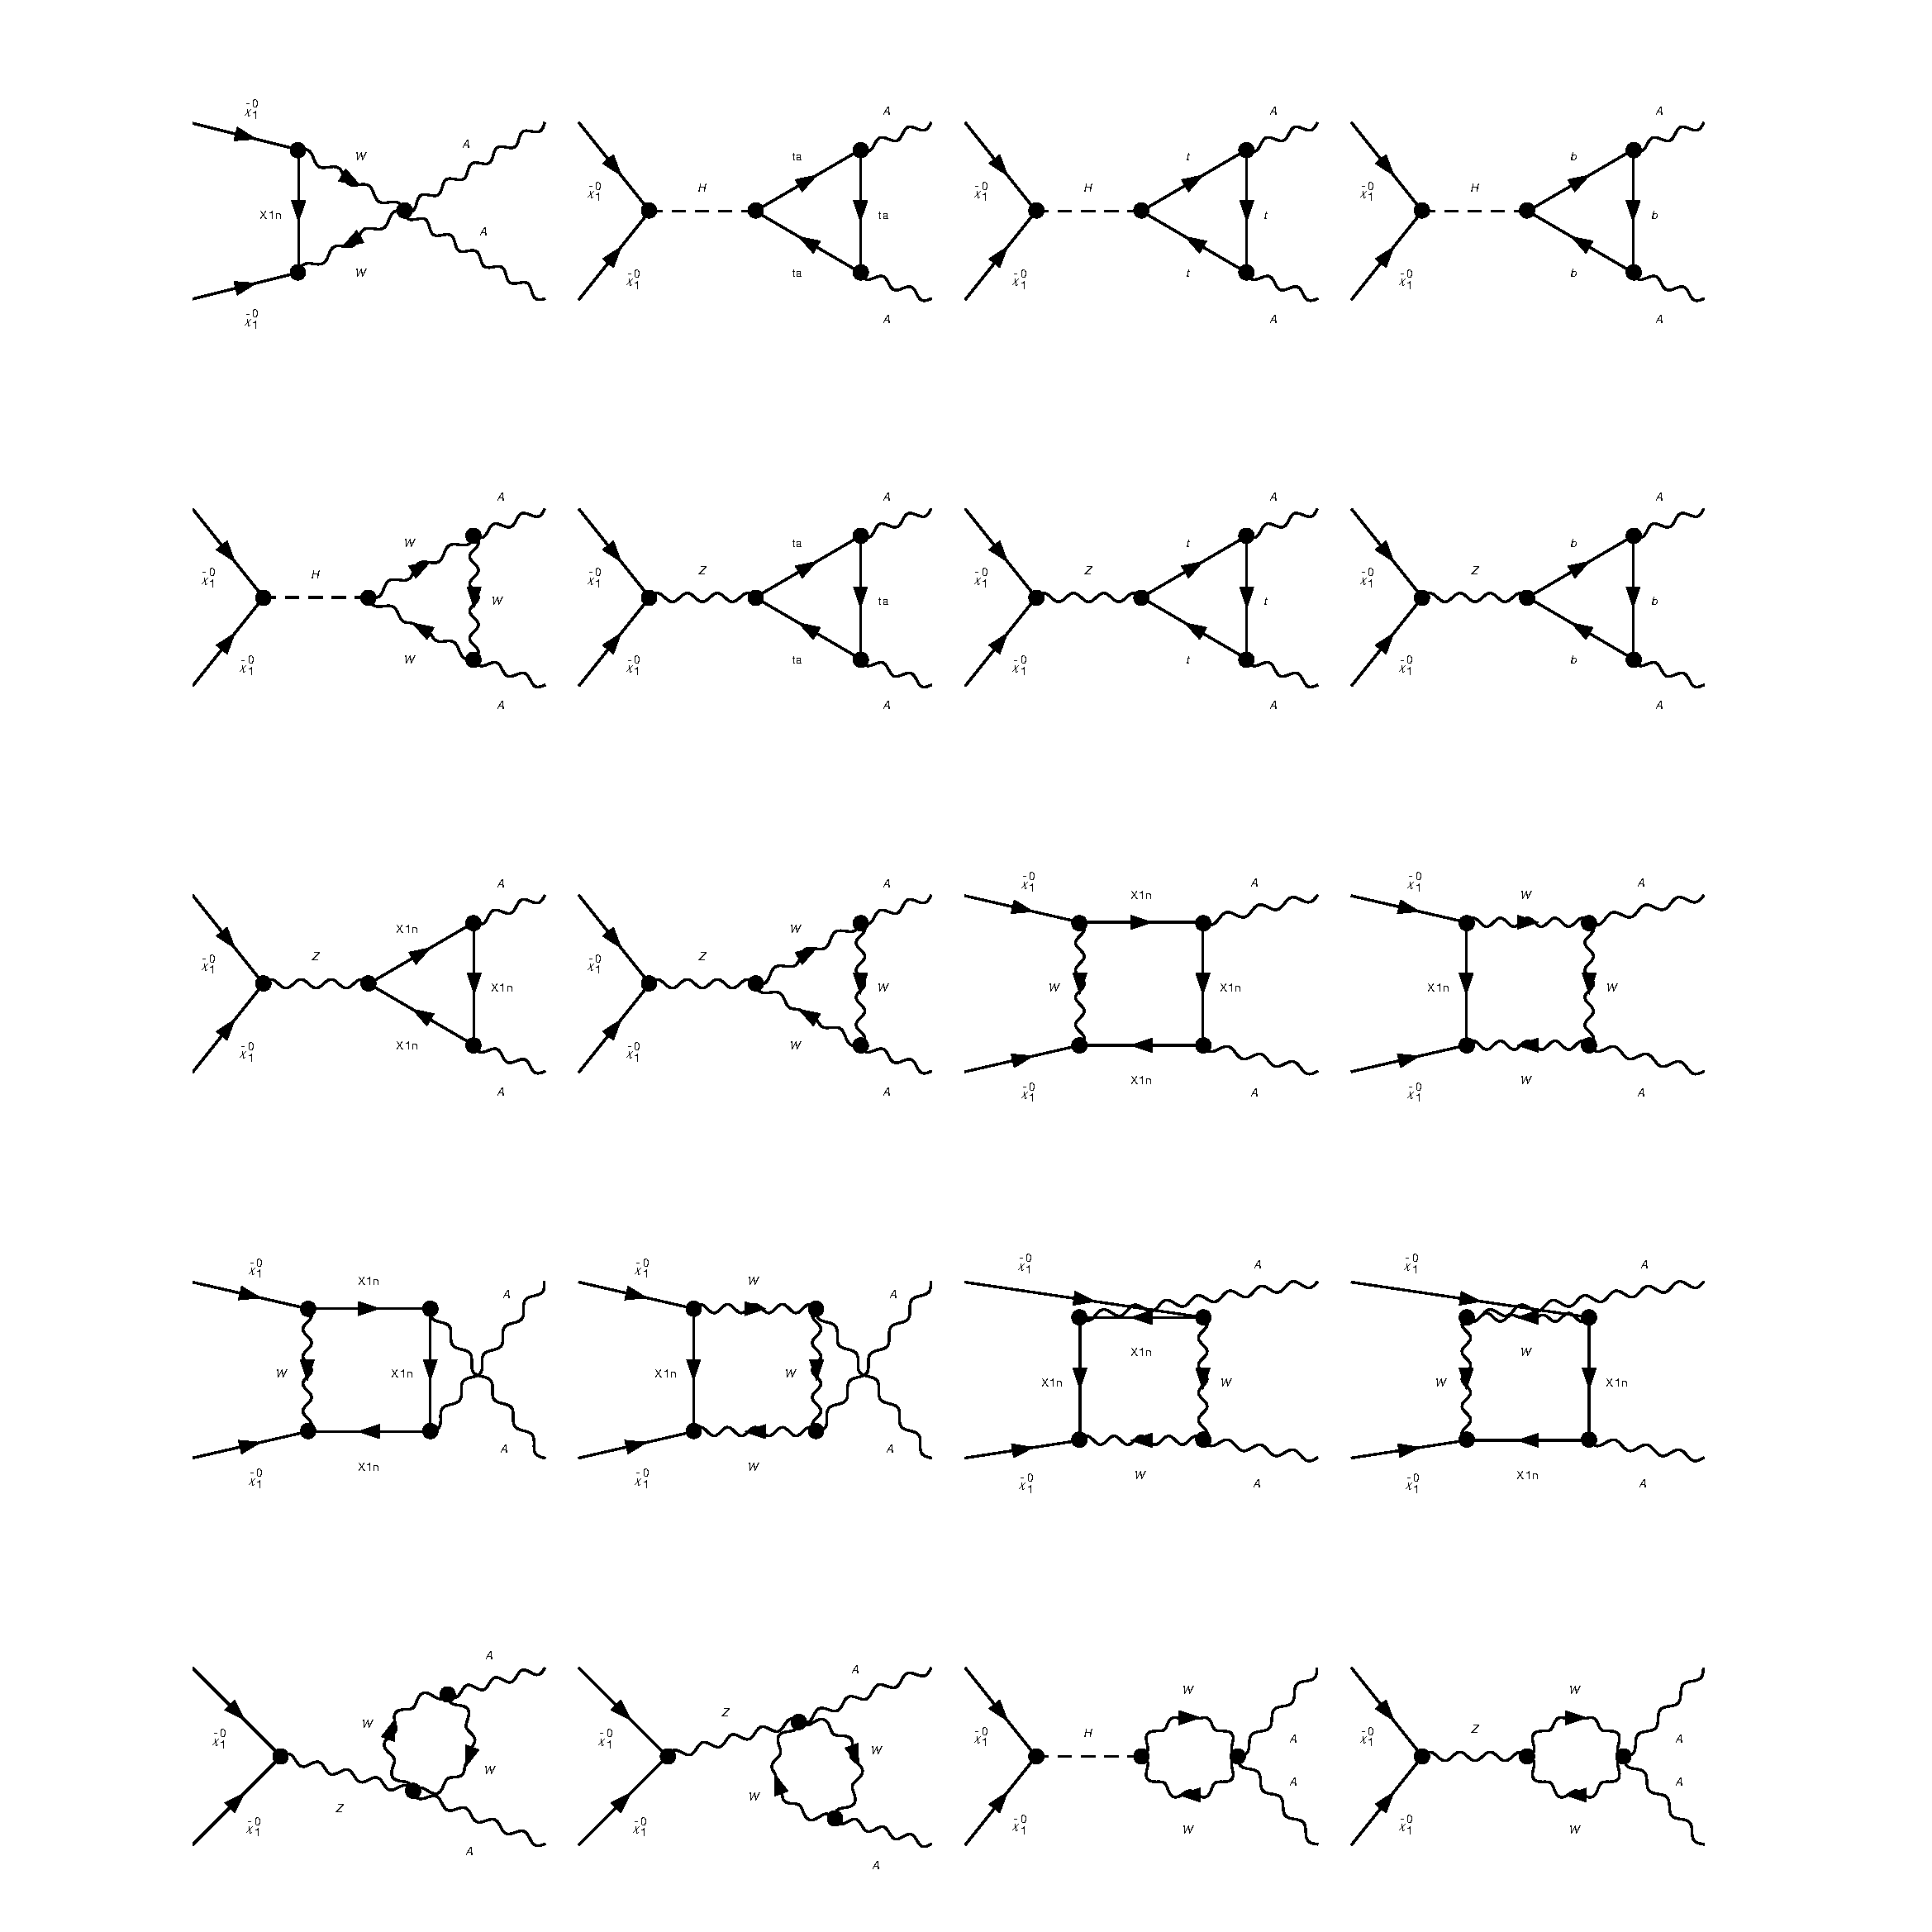
\includegraphics[scale=0.52]{2F-2g-diagrams}
\caption{Feynman diagrams for $\chi^0\chi^0 \to\gamma\gamma$ generated with \textsc{FeynArts}~\cite{Hahn:2000kx}. In order to be more readable we show the diagrams in the unitary gauge. We only used the third family of quarks and one lepton family $\tau= $ ta.  We don't show the equivalent topologies with crossed initial or final state legs.}
\label{fig:2F-to-GG}
\end{figure}
%
%\begin{figure}
%\centering
%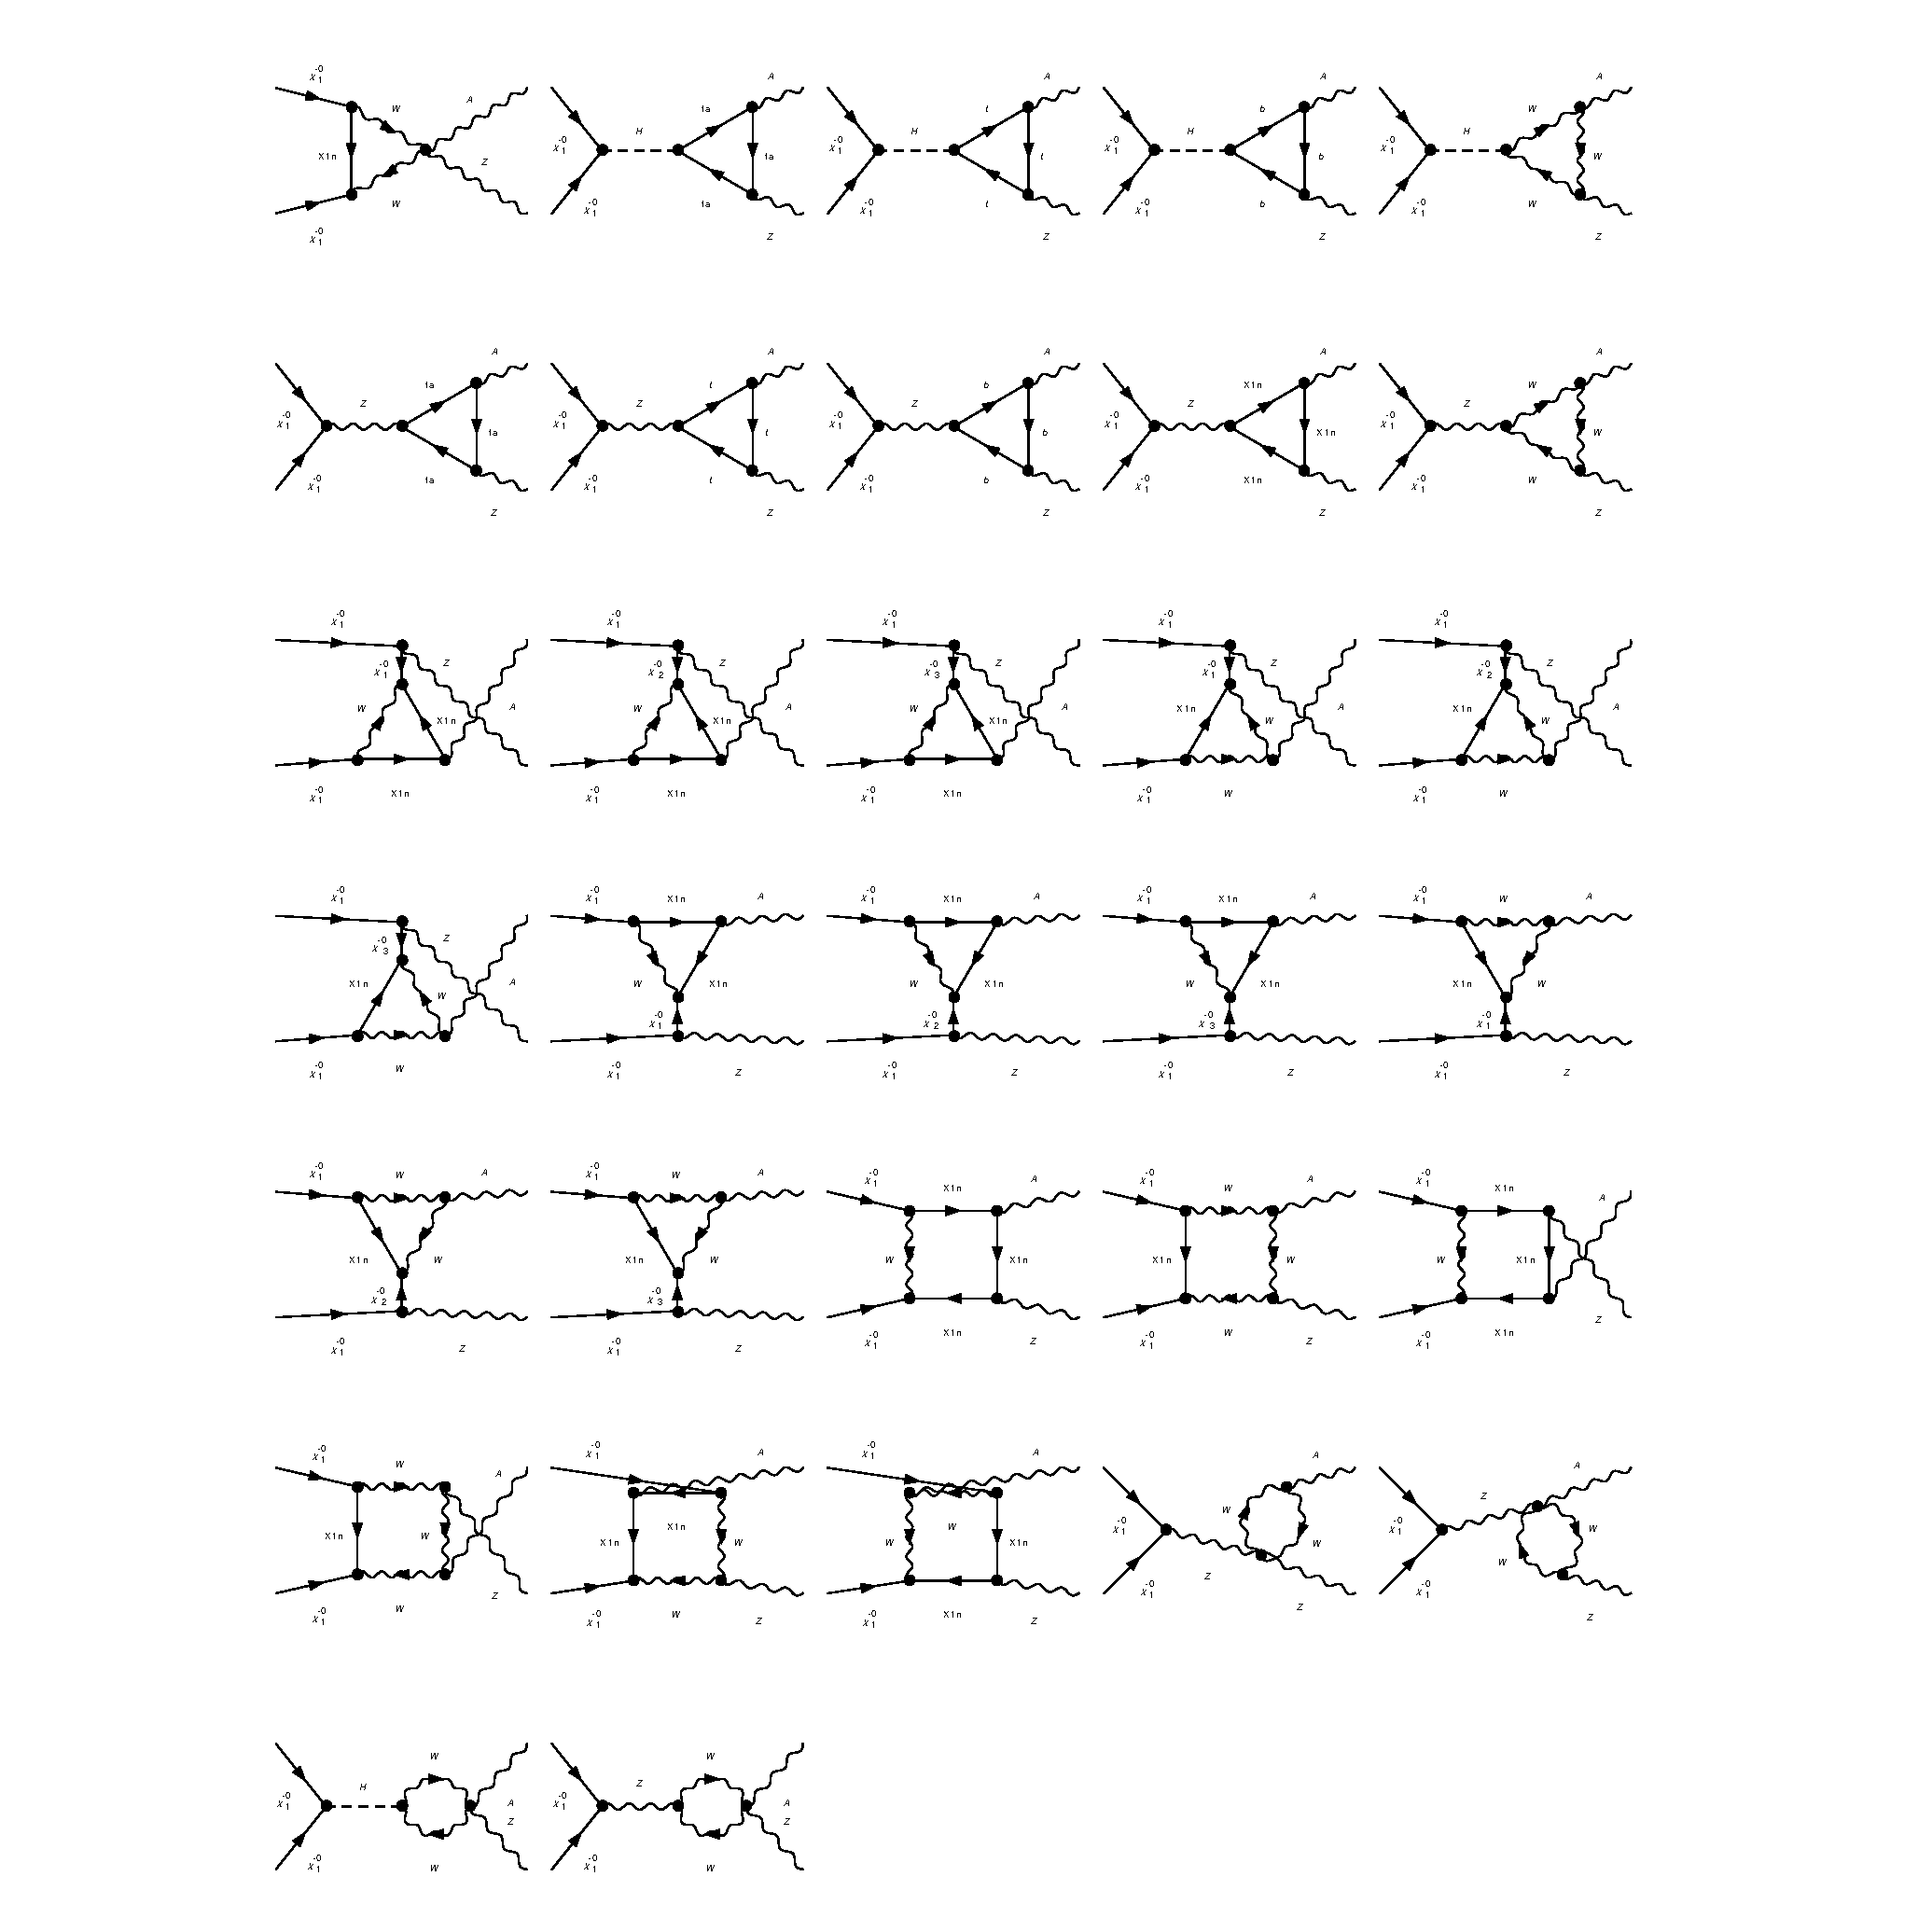
\includegraphics[scale=0.57]{2F-gz-diagrams}
%\caption{Feynman diagrams for $\chi^0\chi^0 \to\gamma Z$ generated with \textsc{FeynArts}~\cite{Hahn:2000kx}. In order to be more readable we show the diagrams in the unitary gauge. We only used the third family of quarks and one lepton family $f$.  We don't show the equivalent topologies with crossed initial or final state legs.}
%\label{fig:2F-to-GZ}
%\end{figure}
%%


%%%%%%%%%%%%%%%%%%%%%%%%%%%%%%%%%%%%%%%%%%%%%%%%%%%%%%%%%
\subsection{Amplitude for fermion DM annihilation}

In the annihilation of the dark matter into two photons show in the Fig.~\ref{fig:annihilationgg}, in general the amplitude is given by
\begin{align}
\label{eq:M1-fermion-GG}
\mathcal{M}_{\gamma\gamma}=\mathcal{M}^{\mu\nu}\epsilon_{\mu}^*(p_3)\epsilon_{\nu}^*(p_4)=\left[\bar{v}_{\sigma 1}\Gamma^{\mu\nu}u_{\sigma 2}\right]\epsilon_{\mu}^*(p_3)\epsilon_{\nu}^*(p_4)\,,
\end{align}
%
where $\Gamma^{\mu\nu}$ comes for the Lorentz structure of the annihilation process, $v_{\sigma 1}$ and $v_{\sigma 2}$ are Dirac spinors for the fermions with spin $\sigma 1,2$ respectively and $\epsilon_{\mu},\epsilon_{\nu}$ are the polarization vectors of the photons. 

In the s-wave limit, the initial state has orbital angular momenta $L=0$ and its wave function $\Psi(p,s)$ must to be antisymmetry because we have two identity fermions in the initial state. Therefore, it must be spin antisymmetry with $S=0$.
%
Considering the wave function $|\Psi_{s=0}\rangle=\tfrac{1}{\sqrt{2}}\left[\uparrow\downarrow|\rangle-|\downarrow\uparrow\rangle\right]$ for the antisymmetry initial state, the amplitude $\mathcal{M^{\mu\nu}}$ in the Eq.~\eqref{eq:M1-fermion-GG} will be given by:
%
\begin{align}
\label{eq:muv}
\mathcal{M}^{\mu\nu}
&=\dfrac{1}{\sqrt{2}}\left[\bar{v}_{\uparrow}\Gamma^{\mu\nu}u_{\downarrow}
-\bar{v}_{\downarrow}\Gamma^{\mu\nu}u_{\uparrow}\right]\nonumber \\
&=\dfrac{1}{\sqrt{2}}\text{Tr}\left[\Gamma^{\mu\nu}u_{\downarrow}\bar{v}_{\uparrow}
-\Gamma^{\mu\nu}u_{\uparrow}\bar{v}_{\downarrow}\right]\,.
\end{align}   
In the last equation we used the properties
\begin{align*}
a^*Mb=\sum_{ij}a_i^*b_j=\sum_{ij}M_{ij}b_ja^*_i=\sum_{ij}M_{ij}(ba^*)_{ji}=\sum_i(Mba^*)_{ii}
=\text{Tr}[Mba^*].
\end{align*}
%
According to the Weyl represestation for the spinors:
\begin{align}
\label{eq:weyl_spinors}
u_{\downarrow}=\sqrt{m}
\begin{pmatrix}
1 \\ 0 \\ 1 \\ 0
\end{pmatrix}\hspace{1 cm}
u_{\uparrow}=\sqrt{m} 
\begin{pmatrix}
0 \\ 1 \\ 0 \\ 1
\end{pmatrix}
\hspace{1.0 cm}
v_{\downarrow}=\sqrt{m}
\begin{pmatrix}
1 \\ 0 \\ -1 \\ 0
\end{pmatrix}\hspace{1 cm}
v_{\uparrow}= -\sqrt{m} 
\begin{pmatrix}
0 \\ 1 \\ 0 \\ -1
\end{pmatrix}\,,
\end{align}
we have
\begin{align}
\mathcal{M}^{\mu\nu}
%=&\tfrac{1}{\sqrt{2}}\text{Tr}\left[\Gamma^{\mu\nu}u_{\downarrow}\bar{v}_{\uparrow}
%-\Gamma^{\mu\nu}u_{\uparrow}\bar{v}_{\downarrow}\right]\nonumber \\
=&\dfrac{m}{\sqrt{2}}\text{Tr}\left[
\Gamma^{\mu\nu}\begin{pmatrix}
0\\1\\0\\1
\end{pmatrix}
(-1)\begin{pmatrix}
0&1&0&-1
\end{pmatrix}\gamma^0 -
\Gamma^{\mu\nu}\begin{pmatrix}
1\\0\\1\\0
\end{pmatrix}
\begin{pmatrix}
1&0&-1&0
\end{pmatrix}\gamma^0
\right] \nonumber\\
=&-\dfrac{m}{\sqrt{2}}\text{Tr}\left[
\Gamma^{\mu\nu}\left\{\begin{pmatrix}
0&0&0&0\\0&1&0&-1\\0&0&0&0\\0&1&0&-1
\end{pmatrix}+\bigg{\}}
\begin{pmatrix}
1&0&-1&0\\0&0&0&0\\1&0&-1&0\\0&0&0&0
\end{pmatrix}
\right\}\gamma^0
\right]\nonumber\\
=&\dfrac{-m}{\sqrt{2}}\text{Tr}
\left[\Gamma^{\mu\nu}\begin{pmatrix}
-1&1\\
-1&1
\end{pmatrix}
\right]
=\dfrac{-m}{\sqrt{2}}\text{Tr}
\left[\Gamma^{\mu\nu}\begin{pmatrix}
-1&0\\
0&1
\end{pmatrix}\left(\begin{pmatrix}
1&0\\0&1
\end{pmatrix}-\begin{pmatrix}
0&1\\1&0
\end{pmatrix}\right)
\right]
\nonumber\\
=&-\dfrac{m}{\sqrt{2}}\text{Tr}\left[\Gamma^{\mu\nu}\gamma^5(1-\gamma^0)\right]\,.
\end{align} 
Therefore, in the s-wave limit where the momentum of the DM is approximately $p\approx (m,0,0,0)$, the amplitude $\mathcal{M}^{\mu\nu}$ will be given by
\begin{align}
\label{eq:projector}
\mathcal{M}^{\mu\nu}=-\dfrac{m}{\sqrt{2}}\text{Tr}\left[\Gamma^{\mu\nu}\gamma^5\left(1-\dfrac{\slashed{p}}{m}\right)\right]
=-\dfrac{m}{\sqrt{2}}\text{Tr}\left[\Gamma^{\mu\nu}\left(1+\dfrac{\slashed{p}}{m}\right)\gamma^5\right]\,,
\end{align}  
where we have shown that the amplitude is been project by the operator~\cite{Bergstrom:1997fh}\,,
\begin{align}
\mathcal{O}_{Ps}=-\dfrac{m}{\sqrt{2}}\left(1+\dfrac{\slashed{p}}{m}\right)\gamma^5\,.
\end{align}

%
In order to compute the amplitude is important to have in mind the relations given in the Tab.~\ref{tab:traza-gammas} for the Dirac $\gamma$-matrices.
%
\begin{table}[h]
\centering
\begin{tabular}{|l|l|}\hline
$\text{Tr}(1)=4$ & $\text{Tr}(\gamma^5)=0$ \\ \hline
$\text{Tr}(\gamma^{\mu})=0$ & $\text{Tr}(\gamma^5\gamma^{\mu})=0$ \\ \hline
$\text{Tr}(\gamma^{\mu}\gamma^{\nu})=4\,g^{\mu\nu}$ & $\text{Tr}(\gamma^5\gamma^{\mu}\gamma^{\nu})=0$ \\ \hline
$\text{Tr}(\gamma^{\mu}\gamma^{\nu}\gamma^{\sigma})=0$ & $\text{Tr}(\gamma^5\gamma^{\mu}\gamma^{\nu}\gamma^{\sigma})=0$ \\ \hline
$\text{Tr}(\gamma^{\mu}\gamma^{\nu}\gamma^{\sigma}\gamma^{\rho})=4\left(g^{\mu\nu}g^{\sigma\rho}-g^{\mu\sigma}g^{\nu\rho}+g^{\mu\rho}g^{\nu\sigma}\right)$ & $\text{Tr}(\gamma^5\gamma^{\mu}\gamma^{\nu}\gamma^{\sigma}\gamma^{\rho})=4\,i\,\epsilon^{\mu\nu\sigma\rho}$ \\ \hline
$\cdots$ & $\cdots$ \\\hline
\end{tabular}
  \caption{Traces of Dirac $\gamma$-matrices.}
  \label{tab:traza-gammas}
\end{table}
%
In general, we know that $\gamma^5=i\gamma^0\gamma^1\gamma^2\gamma^3$ and the trace of odd $\gamma-$matrices are zero. It can be shown to that the trace also vanishes if $\gamma^5$ is accompanied by two $\gamma$-matrices. 

Now, we use the programs \textsc{FeynArts}~\cite{Hahn:2000kx} and \textsc{FormCalc}~\cite{Hahn:1998yk} to compute all the Dirac chains $\left[\bar{v}_{\sigma 1}\Gamma^{\mu\nu}u_{\sigma 2}\right]$ in the Eq.~\eqref{eq:M1-fermion-GG} in order to know the $\Gamma^{\mu\nu}$ tensor elements. Latter, we use the projection operator given in the equation Eq.~\eqref{eq:projector} and in this way  to find an analytic expression for the amplitude $\mathcal{M}^{\mu\nu}$ in the annihilation process. In the Tab.~\ref{tab:dirac-chains} we show the Dirac chains for the The Singlet Doublet Fermion Dark matter model (SDFDM). We noticed, that the chain $[\bar{v}_{k1}\slashed{\epsilon}_3\slashed{\epsilon}_4\slashed{k}_3u_{k2}]$ comes to the boxes diagrams and the others come from triangular diagrams \footnote{$r_3$ and $r_4$ equal to $\pm 1$ depend of the polarization of the photons an will be explain in the Appendix~\ref{sec:polarization-vectors}}. Even more, we notice that all the chains that contribute to the amplitude are proportional to the $\epsilon^{\mu\nu\rho\sigma}$ tensor, and therefore, it can be written as
%
\begin{table}
\centering
\begin{tabular}{|l|c|c|}\hline
& $\chi^0\chi^0\rightarrow\gamma\gamma$ & $\chi^0\chi^0\rightarrow\gamma Z$ \\ \hline \hline
$\bar{v}_{k1}(\mathds{1})u_{k2}$ &  $ 0$ &0 \\ \hline
$-i\epsilon_{\mu\nu\rho\sigma}(\epsilon_3^{\mu}\epsilon_4^{\nu}k_3^{\rho}k_4^{\sigma})[\bar{v}_{k1}\gamma^5u_{k2}]$  & $ -\tfrac{4m^3}{\sqrt{2}}(r_3+r_4)$ &
$\tfrac{-m}{\sqrt{2}}(4m^2-m_Z^2)(r_3+r_4)$\\ \hline 
$[\bar{v}_{k1}\slashed{k}_3u_{k2}]$  & $ 0$ &0\\ \hline 
$-i\epsilon_{\mu\nu\rho\sigma}(\epsilon_3^{\mu}\epsilon_4^{\nu}k_3^{\rho}k_4^{\sigma})[\bar{v}_{k1}\gamma^5\slashed{k}_3u_{k2}]$  & $-\tfrac{4m^4}{\sqrt{2}}(r_3+r_4)$ &
$\tfrac{-m^2}{\sqrt{2}}(4m^2-m_Z^2)(r_3+r_4)$\\ \hline 
$[\bar{v}_{k1}\slashed{\epsilon}_3\slashed{\epsilon}_4u_{k2}]$  &$ 0$ &0\\ \hline 
$[\bar{v}_{k1}\slashed{\epsilon}_3\slashed{\epsilon}_4\slashed{k}_3u_{k2}]$ 
$=-i\sqrt{2}\epsilon_{\mu\nu\rho\sigma}k_3^{\rho}k_4^{\sigma}\epsilon_3^{\nu}\epsilon_4^{\rho}$  & $\tfrac{2m^2}{\sqrt{2}}(r_3+r_4)$ & $ -\tfrac{1}{2\sqrt{2}}(m_Z^2-4m^2)(r_3+r_4)$  \\ \hline 
$-i\epsilon_{\mu\nu\rho\sigma}(\epsilon_3^{\nu}\epsilon_4^{\rho}k_1^{\sigma})[\bar{v}_{k1}\gamma^{\mu}u_{k2}]$  & $ 0$ & 0\\ \hline 
$-i\epsilon_{\mu\nu\rho\sigma}(\epsilon_3^{\nu}\epsilon_4^{\rho}k_1^{\sigma})[\bar{v}_{k1}\gamma^5\gamma^{\mu}u_{k2}]$  & $ 0$ & 0\\ \hline 
$-i\epsilon_{\mu\nu\rho\sigma}(\epsilon_3^{\nu}\epsilon_4^{\rho}k_2^{\sigma})[\bar{v}_{k1}\gamma^{\mu}u_{k2}]$  & $ 0$ &0\\ \hline 
$-i\epsilon_{\mu\nu\rho\sigma}(\epsilon_3^{\nu}\epsilon_4^{\rho}k_2^{\sigma})[\bar{v}_{k1}\gamma^5\gamma^{\mu}u_{k2}]$  & $ 0$ & 0\\ \hline 
$-i\epsilon_{\mu\nu\rho\sigma}(\epsilon_3^{\nu}\epsilon_4^{\rho}k_3^{\sigma})[\bar{v}_{k1}\gamma^{\mu}u_{k2}]$  & $0$ & 0\\ \hline 
$-i\epsilon_{\mu\nu\rho\sigma}(\epsilon_3^{\nu}\epsilon_4^{\rho}k_3^{\sigma})[\bar{v}_{k1}\gamma^5\gamma^{\mu}u_{k2}]$  & $ \tfrac{2m^2}{\sqrt{2}}(r_3+r_4)$ & 
$\tfrac{1}{2\sqrt{2}}(4m^2-m_Z^2)(r_3+r_4)$\\ \hline 
$-i\epsilon_{\mu\nu\rho\sigma}(\epsilon_3^{\nu}\epsilon_4^{\rho}k_4^{\sigma})[\bar{v}_{k1}\gamma^{\mu}u_{k2}]$  & $0$ & 0 \\ \hline 
$-i\epsilon_{\mu\nu\rho\sigma}(\epsilon_3^{\nu}\epsilon_4^{\rho}k_4^{\sigma})[\bar{v}_{k1}\gamma^5\gamma^{\mu}u_{k2}]$  & $-\tfrac{2m^2}{\sqrt{2}}(r_3+r_4)$ &
$-\tfrac{1}{2\sqrt{2}}(4m^2-m_Z^2)(r_3+r_4)$\\ \hline 
\end{tabular}
  \caption{Dirac chains and the projection for the DM self-annihilation into $\gamma\gamma$ and $\gamma Z$. In this notation of \textsc{FormCalc}, $k_i=p_i$.}
  \label{tab:dirac-chains}
\end{table}

\begin{align}
\label{eq:M-fermion-GG}
\mathcal{M}_{\gamma\gamma}=\mathcal{A}_{\gamma\gamma}\,\epsilon^{\mu\nu\sigma\rho}p_{3\sigma}p_{4\rho}\,\epsilon_{\mu}^*(p_3)\epsilon_{\nu}^*(p_4)\,,
\end{align}
%
how is expected by the invariance under the $CP$ symmetry, because we know that the initial state is $CP$ odd for a Majorana fermion \footnote{$ CP(\chi^0)=i \Rightarrow CP(\chi^0\chi^0)=-1$.} and the only tensor in the Lorentz group that is odd under $CP$ is the Levi-Civita tensor $\epsilon^{\mu\nu\sigma\rho}$.

On the other hang, for the DM annihilation into $\gamma Z$, we have
\begin{align}
\label{eq:M-fermion-GZ}
\mathcal{M}_{\gamma Z}=\mathcal{A}_{\gamma Z}\,\epsilon^{\mu\nu\sigma\rho}p_{3\sigma}p_{4\rho}\,\epsilon_{\mu}^*(p_3)\epsilon_{\nu}^*(p_4)\,,
\end{align}
%
where $\mathcal{A}_{\gamma Z}$ is the corresponding form factor.

As we described for the case of the scalar DM, when \textsc{FeynArts}~\cite{Hahn:2000kx} and \textsc{FormCalc}~\cite{Hahn:1998yk} compute the amplitudes $\mathcal{M}_{\gamma\gamma}$ and $\mathcal{M}_{\gamma Z}$ we get an big expression that in general depend of the Passarino Veltman one loop integrals that we describe in the Appendix~\ref{sec:passarino-veltman}. Numerically, we can evaluated this expression using \textsc{LoopTools}~\cite{Hahn:1998yk}. However, our goal is to get an analytical result and for that reason we implement the algorithm that we describe in the Appendix~\ref{sec:CD-reduction} in order to reduce the Passarino Veltman integrals of the \textsc{FormCalc} output.
%
The algorithm reduce the fourth-point function to three point functions and all the coefficients tensor of the loop integrals. Usually, the results are given in terms of the scalar Passarino Veltman $C_0$ which can be written in terms of the dilogarithm Li$_{2}$ function. In this case, the notation is more compact and readable.

The amplitudes $\mathcal{M}_{\gamma\gamma}$ and $\mathcal{M}_{\gamma Z}$ obtained where:


\begin{align}
\label{eq:M-FFGG}
&\mathcal{M}_{\gamma\gamma}=\mathcal{M}_{\gamma\gamma}^{SM}+\mathcal{M}_{\gamma\gamma}^{box}\,
\end{align}
where,
\begin{align}
\label{eq:M-FFGG1}
\mathcal{M}_{\gamma\gamma}^{SM}
=&-\dfrac{2 \sqrt{2} \alpha^2 m^2 (N_{21}^2 - N_{31}^2)
(-4 + 4 \sin^2\theta_W - \epsilon) }{3(4 m^2 - M_Z^2) \sin^2\theta_W  (-1 + \sin^2\theta_W ) \epsilon}
(r_3+r_4)\bigg{\{}
m_b^2C_0(4 m^2,0,0, m_b^2, m_b^2, m_b^2)\nonumber\\
-&4m_t^2C_0(4 m^2,0,0, m_t^2, m_t^2, m_t^2)+3m_{\tau}^2C_0(4 m^2,0,0, m_{\tau}^2, m_{\tau}^2, m_{\tau}^2)
\bigg{\}}
\end{align}
%
\begin{align}
\label{eq:M-FFGG2}
\mathcal{M}_{\gamma\gamma}^{box}&
=-\dfrac{\alpha}{\pi}\dfrac{ g^2 m^2}{2 \sqrt{2}}(r_3+r_4)
\bigg{\{}
\dfrac{8 (N_{21}^2 + N_{31}^2)(-1 +\epsilon)}{(-1 - u + \epsilon)}C_0(4 m^2,0,0, m_W^2, m_W^2, m_W^2)\nonumber\\
-&\dfrac{2\sqrt{u}(-2 N_{21} N_{31}(-1 + u - 4 \epsilon) 
-(N_{21}^2+N_{31}^2)\sqrt{u}(-1 + u - 2 \epsilon) }{(-1 + u - \epsilon) \epsilon}C_0(4 m^2,0,0, M_D^2, M_D^2, M_D^2)\nonumber\\
+& \dfrac{\left[12 N_{21}N_{31}\sqrt{u}(1+u-\epsilon)+(N_{21}^2+N_{31}^2)(1+u^2 +u(-6 +\epsilon)+\epsilon -
2 \epsilon^2)\right]}{(u-\epsilon)(1+u-\epsilon)}C_0(0,m^2,-m^2,m_W^2, m_W^2, M_D^2)\nonumber\\
+&\dfrac{\sqrt{u} (12 N_{21} N_{31} \epsilon + (N_{21}^2 +N_{31}^2)\sqrt{u} (1 + u^2 + u (-2 + \epsilon) - 3 \epsilon - 2 \epsilon^2) )}{(-1 + u - \epsilon) (u - \epsilon)\epsilon}C_0(0,m^2,-m^2,M_D^2, M_D^2, m_W^2)
\bigg{\}}\,
\end{align}
%

%
where $\epsilon=m_W^2/m^2 $ , $ u=M_D^2/m^2$ and $r_{3,4}$ are the polarization of final states.
%
\begin{align}
\label{eq:M-FFGZ}
\mathcal{M}_{\gamma Z}=
\end{align}

{\color{red} in proces}













%%%%%%%%%%%%%%%%%%%%%%%%%%%%%%%%%%%%%%%%%%%%%%%%%%%%%%%%%%%%%%%%%%%%%%%%%%%%%%%%%%%%%%%%%%%%%%%%%%%%%
\subsection{Velocity averaged annihilation cross section $\langle \sigma v \rangle$ for fermion DM annihilation into $\gamma\gamma$ and $\gamma Z$}

As we did for the scalar case, the thermal velocity averaged annihilation cross section for the case of fermion DM annihilation into two photons~Fig.\ref{fig:annihilationgg} it is given by
%
\begin{align}
\langle\sigma v_r\rangle=&\dfrac{1}{32\pi\, m^2}\overline{{|\mathcal{M}_{\gamma\gamma}|^2}}\left(1-\dfrac{v_r^2}{8}+\mathcal{O}(v_r^4)\right)\,,
\end{align}
thus, using the Appendix~\ref{sec:sigmav}, the s-wave contribution is
\begin{align}
\langle\sigma v_r\rangle\Big{\vert}_{\text{s-wave}}
=&\dfrac{1}{32\pi\, m^2}\overline{{|\mathcal{M}_{\gamma\gamma}|^2}}
=\dfrac{1}{32\pi\, m^2}\dfrac{1}{2}\sum_{r_3r_4=\pm 1}\dfrac{1}{4}\sum_{s_3s_4}{|\mathcal{M}_{\gamma\gamma}|^2} \,,
\end{align}
%
where $r_{3,4}$ are the polarization of final states, $s_{3,4}$ are the spin of the initial fermions and the amplitude $\mathcal{M}_{\gamma\gamma}$ is given by Eq.~\eqref{eq:M-FFGG}.

For the case of fermion DM annihilation into one photon and one $Z$ gauge boson~Fig.\ref{fig:annhilation-gz} we have
%
\begin{align}
\langle\sigma v_r\rangle
= &  \dfrac{1}{32\pi\, m^2}\left[ 1- \left(\dfrac{m_Z}{2m}\right)^2 +\dfrac{1}{8}\left(-1+3\left(\dfrac{m_Z}{2m}\right)^2\right) v_r^2 + \mathcal{O}(v_r^4)\right]\overline{{|\mathcal{M}_{\gamma Z}|^2}} \,.
\end{align}
%
Thus, using the Appendix~\ref{sec:sigmav}, the s-wave contribution is
\begin{align}
\langle\sigma v_r\rangle\Big{\vert}_{\text{s-wave}}
= & \dfrac{1}{32\pi\, m^2}\left( 1- \dfrac{m_Z^2}{4m^2} \right)\overline{{|\mathcal{M}_{\gamma Z}|^2}} 
=\dfrac{1}{32\pi\, m^2}\left( 1- \dfrac{m_Z^2}{4m^2} \right)\sum_{r_3r_4}\dfrac{1}{4}\sum_{s_3s_4}|\mathcal{M}_{\gamma Z}|^2
\end{align}
%
where $r_{3,4}$ are the polarization of final states, $s_{3,4}$ are the spin of the initial fermions and the amplitude $\mathcal{M}_{\gamma Z}$ is given by Eq.~\eqref{eq:M-FFGZ}.





%%%%%%%%%%%%%%%%%%%%%%%%%%%%%%%%%%%%%%%%%%%%%%%%%%%%%%%%%%%%%%%%%%%%%%%%%%%%%%%%%%%%%%%%%%%%
\subsection{ Matrix of gauge contribution to gamma rays }
%
In the SDFDM model the DM is a composition of the gauge eigenstates $\boldsymbol{\Xi}_i^0$ Eq.~\eqref{eq:rotation} such that $\chi_1=N_{11}N+N_{21}\psi_L^0+N_{31}{\psi_R^0}^{\dagger}=N_{i1}\boldsymbol{\Xi}_i^0$. For that reason, the amplitudes of DM annihilation into $\chi_1\chi_1\to\gamma\gamma$ or $\chi_1\chi_1\to\gamma Z$ must to have the form 
\begin{align}
\mathcal{M}=\langle\chi_1|\Gamma^{\mu\nu}\epsilon_{\mu}\epsilon_{\nu}|\chi_1\rangle
=\sum_{ij}N_{i1}N_{j1}\langle\boldsymbol{\Xi}_i^0|\Gamma^{\mu\nu}\epsilon_{\mu}\epsilon_{\nu}|\boldsymbol{\Xi}_i^0\rangle
=\sum_{ij}N_{i1}N_{j1}\langle\boldsymbol{\Xi}_i^0|\Gamma|\boldsymbol{\Xi}_j^0\rangle\,.
\end{align}
According to the last equation, we can extract the Bino $N=\boldsymbol{\Xi}_1^0$ or the Higgsino $\psi_{L}^0=\boldsymbol{\Xi}_2^0$, ${\psi_{R}^0}^{\dagger}=\boldsymbol{\Xi}_3^0$ components that contribute to the process. Even more,  we know that a pure Bino contribution to the scattering must to be zero because the Bino itself do not couple to the gauge bosons and only must to remains the $SU(2)$ gauge contribution. In order to take this in account, we construct the symmetry matrix $\mathcal{R}$ witch in the case of DM annihilation into photons is given by
%
\begin{align}
\label{eq:Dmatrix}
\mathcal{R}_{ij}
=&\begin{pmatrix}
NN\to\gamma\gamma & N\psi_L^0\to\gamma\gamma & N\psi_R^0\to\gamma\gamma\\
\psi_LN\to\gamma\gamma & \psi_L\psi_L^0\to\gamma\gamma & \psi_L\psi_R^0\to\gamma\gamma\\
\psi_R^0N\to\gamma\gamma & \psi_R^0\psi_L^0\to\gamma\gamma & \psi_R^0\psi_R^0\to\gamma\gamma
\end{pmatrix}\nonumber\\
=&\dfrac{\partial}{\partial N_{i1}}\dfrac{\partial}{\partial N_{j1}}\mathcal{M}
=\dfrac{\partial}{\partial N_{i1}}\dfrac{\partial}{\partial N_{j1}}\sum_{kl}N_{k1}N_{l1}\langle\boldsymbol{\Xi}_k| \Gamma|\boldsymbol{\Xi}_l\rangle 
=\begin{pmatrix}
0  & 0 & 0 \\
0 & \dfrac{\partial^2}{\partial N_{21}^2}\mathcal{M} & \dfrac{\partial}{\partial N_{21}}\dfrac{\partial}{\partial N_{31}}\mathcal{M} \\
0 & \dfrac{\partial}{\partial N_{31}}\dfrac{\partial}{\partial N_{21}}\mathcal{M} & \dfrac{\partial^2}{\partial N_{31}^2}\mathcal{M} 
\end{pmatrix}\,.
\end{align}
%
$\mathcal{R}_{22}$ and $\mathcal{R}_{33}$ gives us the contribution to the amplitude coming from the gauge $SU(2)$ components $\psi_L^0$ and ${\psi_R^0}^{\dagger}$ respectively, and $\mathcal{R}_{23}$ gives us a possible contribution coming from the mixing term $\psi_L^0{\psi_R^0}^{\dagger}$.
\\
We compute the $\mathcal{R}_{ij}$ matrix  using \textsc{FeynArts}~\cite{Hahn:2000kx} and \textsc{FormCalc}~\cite{Hahn:1998yk} and checked that $\mathcal{R}_{22}=\mathcal{R}_{33}$  in the case when we take the SM without fermions. We understood this because $\psi_L^0$ and ${\psi_R^0}^{\dagger}$ are the two components of one vector like $SU(2)$ doublet fermion which components couple in the same way to the SM fermions. In order to check that, we used the relations 
\begin{align}
\lambda_u =& \dfrac{(m_1N_{31} - N_{21}M_D)}{N_{11}}\dfrac{\sqrt{2}}{v} \nonumber\\ 
\lambda_d =& \dfrac{(-m_1N_{21} + N_{31}M_D)}{N_{11}}\dfrac{\sqrt{2}}{v}\,,
\end{align}
in order to simplified the analytically expression.









%%%%%%%%%%%%%%%%%%%%%%%%%%%%%%%%%%%%%%%%%%%%%%%%%%%%%%%%%%%%%%%%%%%%%%%%%%%%%%%%%%%%%%%%%%%%%%%%%%%%%%
%\subsection{Diagrams in the unitary gauge}
%%
%\begin{figure}
%\centering
%\includegraphics[scale=0.46]{gg1}
%\includegraphics[scale=0.46]{gg2}
%\caption{Feynman diagrams for annihilation into two photons in unitary gauge.}
%\end{figure}
%%
%\begin{figure}
%\centering
%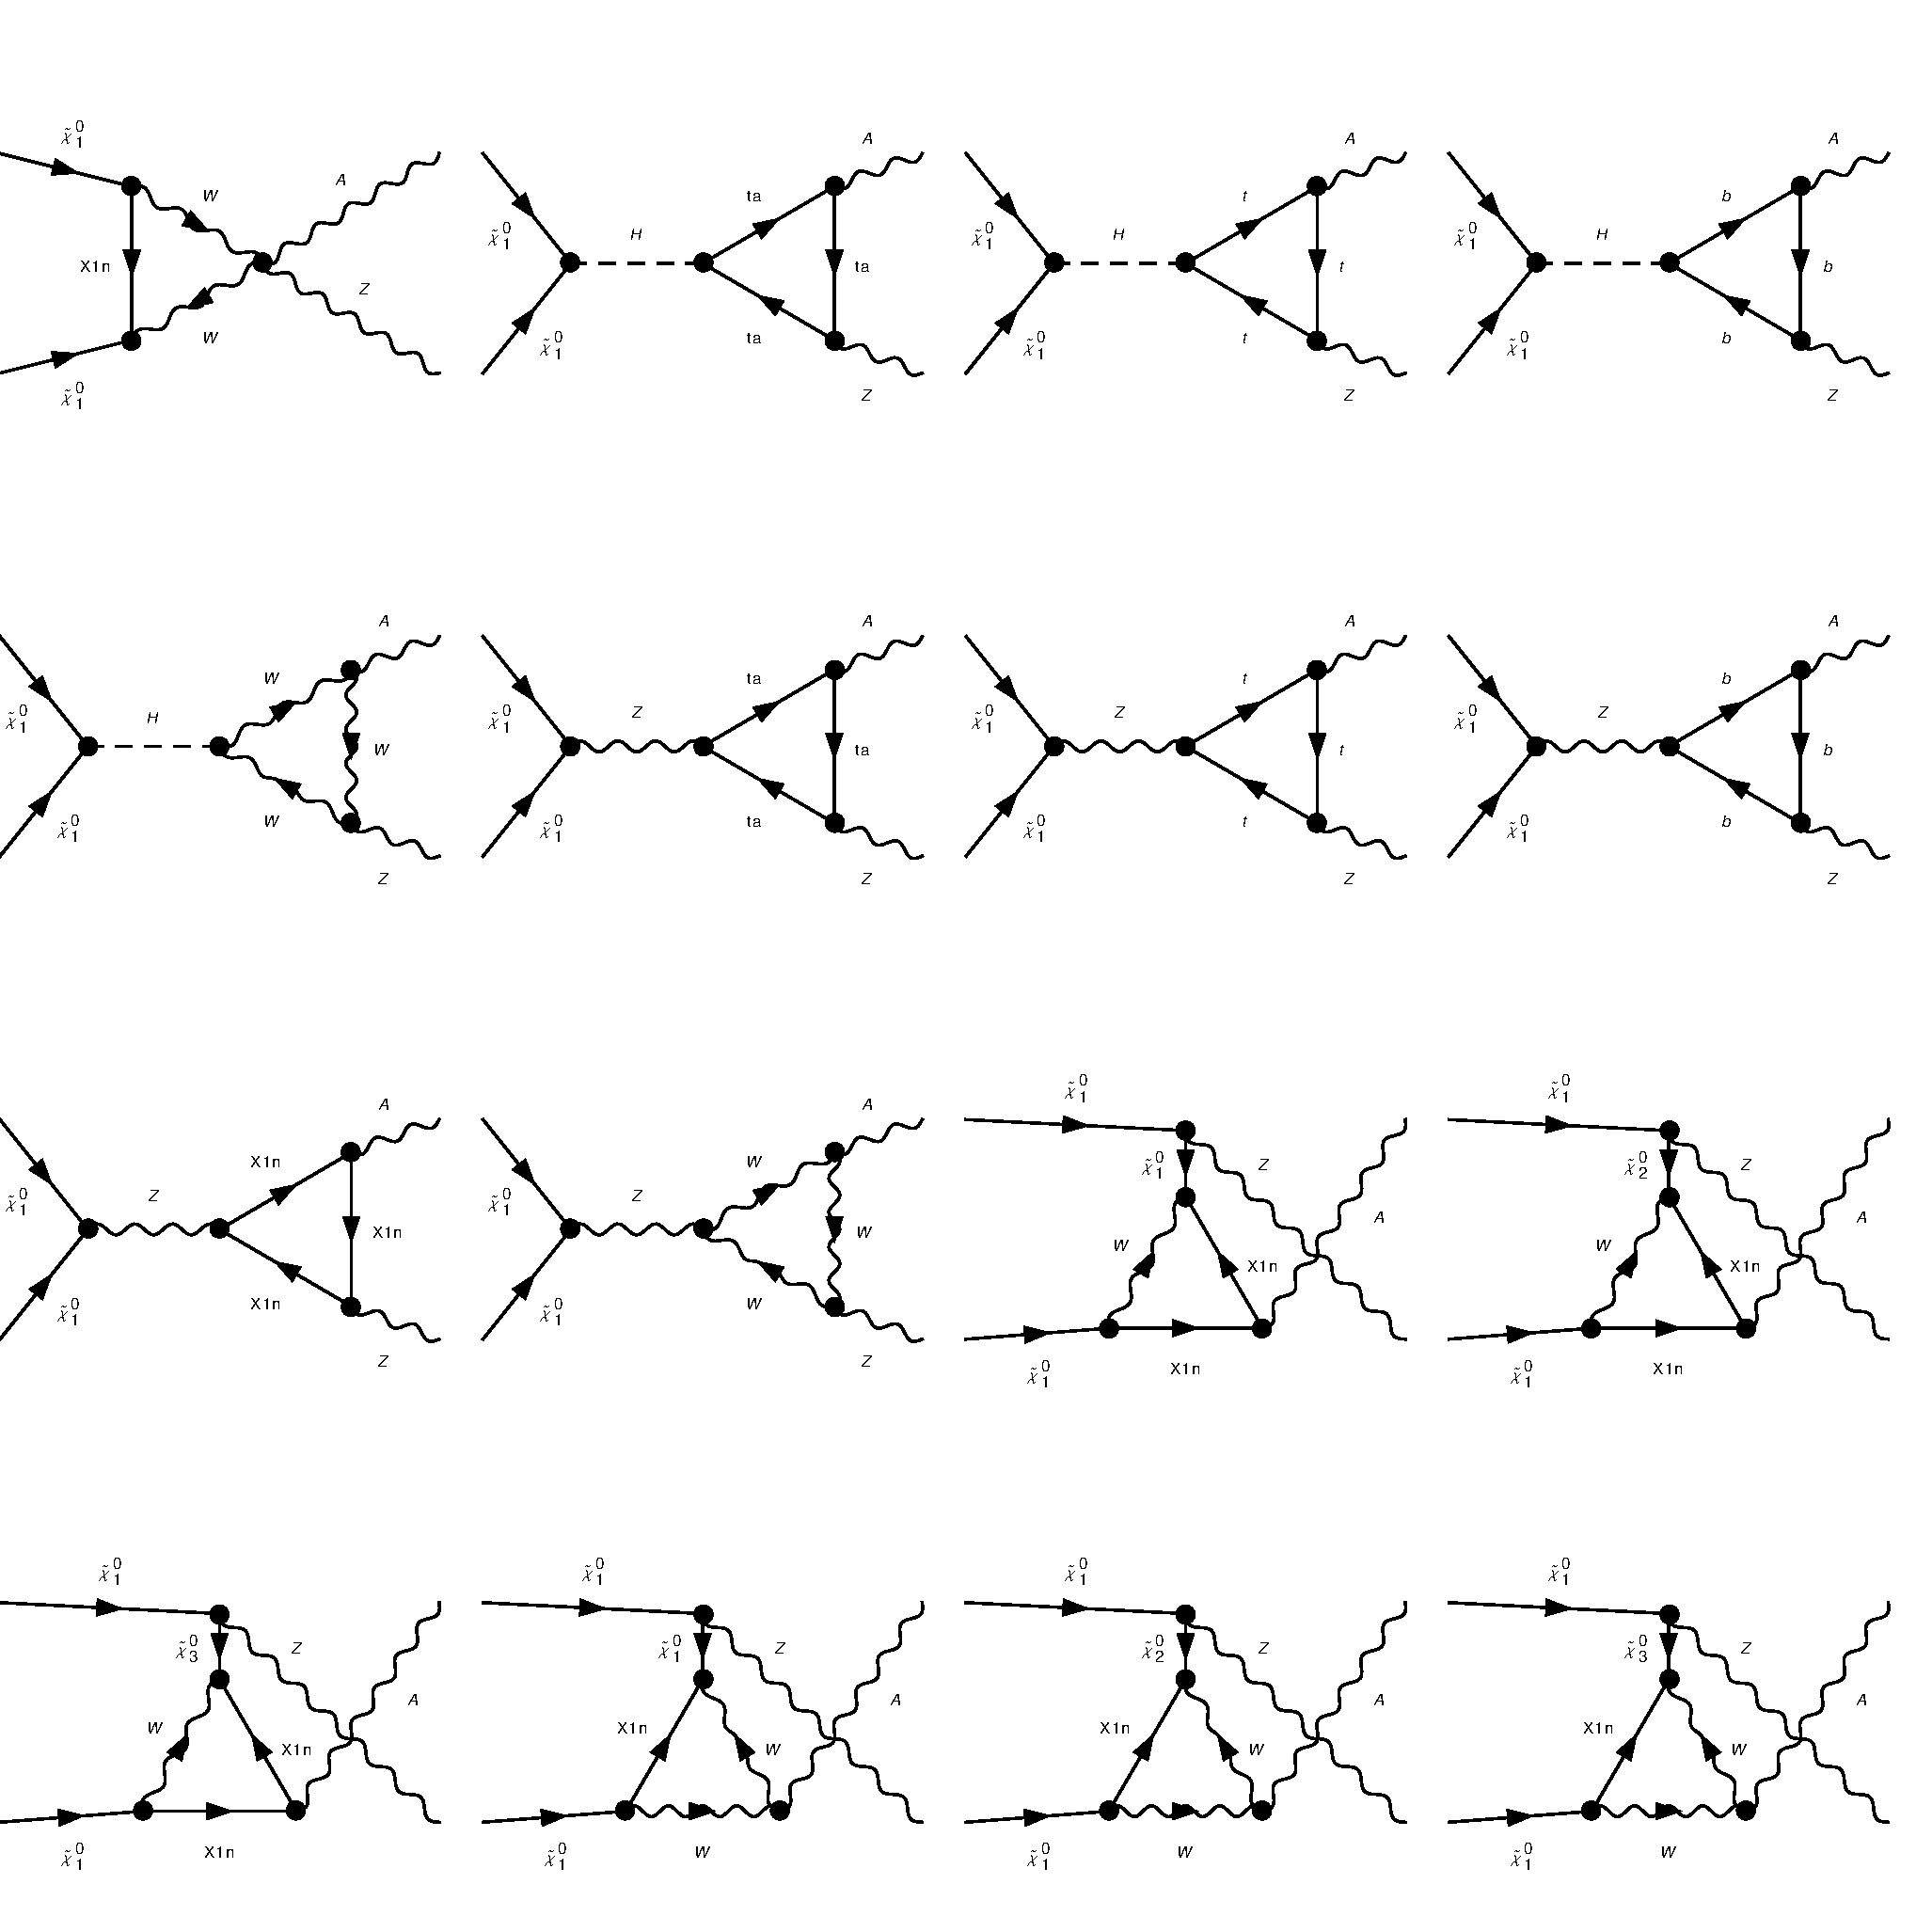
\includegraphics[scale=0.46]{gz1}
%\end{figure}
%%
%\begin{figure}
%\centering
%\includegraphics[scale=0.46]{gz2}
%\caption{Feynman diagrams for annihilation into $\gamma Z$ in unitary gauge.}
%\end{figure}
%%
%
%\chapter*{Conclusions\markboth{Conclusions}{Conclusions}}
%\label{sec:Conclusions}
%\addcontentsline{toc}{chapter}{Conclusions}
%\section{For the SDFDM model with scalars}
We have combined the singlet-doublet fermion dark matter (SDFDM) and
the singlet scalar dark matter (SSDM) models into a framework that generates radiative neutrino masses. 
The required lepton number violation only happens if the scalars are
real.   
We have then explored the novel features of the final model in flavor
physics, collider searches, and dark matter related experiments.  
In the case of SSDM, for example, the singlet-doublet fermion mixing
cannot be too small in order to be compatible with lepton flavor
violating (LFV) observables like $\operatorname{Br}(\mu\to e\gamma)$,
while in the case of fermion dark matter the LFV constraints are
automatically satisfied.
The presence of new decay channels for the next to lightest odd
particle opens the possibility of new signals at the LHC.
In particular, when the singlet scalar is the lightest
odd-particle and the singlet-like Majorana fermion is heavier than the
charged Dirac fermion, the production of the later yields dilepton plus missing transverse energy signals. For large enough
$e^\pm$ or $\mu^\pm$ branchings, these signals could exclude charged
Dirac fermion masses
of order $\SI{500}{GeV}$ in the Run I of the LHC. 
Finally, the effect of coannihilations with the scalar singlets was
studied in the case of doublet-like fermion dark matter.  In that
case, it is possible to obtain the observed dark matter relic density
with lower values of the LOP mass.


\section{For the GCE}
In this work we have entertained the possibility of finding model points in the SDFDM model that can explain the GCE while being in agreement with a multitude of different direct and indirect DM detection constrains. We found two viable regions: (i) DM particles present in the model with masses of $\sim 99$ GeV annihilating mainly into $W$ bosons with branching ratios greater than $\sim 70\%$, (ii) and a second region where the DM particle mass is in the range $\sim (173-190)$ GeV annihilating predominantly into the $t\bar{t}$ channel with branching ratios greater than $\sim 90\%$. Our analysis assumed that the DM is made entirely out of the lightest stable particle $\chi^0$ of the SDFDM model. Despite this being a very restrictive assumption, we have demonstrated that there exist models capable of accounting for the GeV excess in the GC that can be fully tested by the forthcoming XENON-1T and LZ experiments as well as by future \textit{Fermi}-LAT observations in dwarf galaxies. Interestingly, the most recent limits presented by LUX are able to probe a fraction of the good fitting models to the GCE found in this work. We also showed through realistic calculations of CTA performance when observing the GC that this instrument will not have the ability to confirm the SDFDM model if it is causing the GCE.
%
%%%%APENDIX
%\appendix\chapter{Lagrangian in the T13A model}
%

\section{The model}
 The particle content consist of two $SU(2)_L$-doublets vector-like
 Weyl fermions of opposite hypercharges $\eta_u$, $\eta_d$; one singlet
 Weyl fermion of zero hypercharge $N$, and three of singlet real
 scalars of zero hypercharges. All of them odd under some $Z_2$
 symmetry.

\section{Preliminars}

Weyl spinors tranform under Lorentz as shown in Table~\ref{tab:electron}, illustrated for the case of the electron.

\begin{table}
  \centering
  \begin{tabular}{llll}
    Name & Symbol & Lorentz & $U(1)_Q$\\\hline
   $e_L^-$: left electron & $\xi_{\alpha}$ & ${M_{\alpha}}^{\beta}$ & $e^{i\theta}$\\
   $\left( e_L^- \right)^{\dagger}$: right positron    & $\left( \xi_{\alpha} \right)^{\dagger}=\xi^{\dagger}_{\dot{\alpha}}$ & ${{M^{*}}_{\dot{\alpha}}}^{\dot{\beta}}$ & $e^{-i\theta}$\\
   $e_R$: right electron   & $\left( \eta^{\alpha} \right)^{\dagger}=\eta^{\dagger\;\dot{\alpha}}$ & ${\left[ \left( M^{-1} \right)^\dagger \right]^{\dot{\alpha}}}_{\dot{\beta}}$& $e^{i\theta}$\\
   $\left( e_R^{-} \right)^{\dagger}$: left positron &$\eta^{\alpha}$& ${\left[ \left( M^{-1} \right)^T \right]^{\alpha}}_{\beta}$ & $e^{-i\theta}$\\\hline
  \end{tabular}
  \caption{Electron components}
  \label{tab:electron}
\end{table}



\section{Weyl spinors}
Consider the following set of Weyl spinor
\begin{align*}
  L=&
  \begin{pmatrix}
  \xi_{1\alpha}\\
  \xi_{2\alpha}
  \end{pmatrix}
  =
  \begin{pmatrix}
  \nu_L\\
  e_L    
  \end{pmatrix}&
  N=&\eta_1^{\alpha} \nonumber\\
  R_u=&
  \begin{pmatrix}
  \eta_2^{\dagger\dot{\alpha}}\\
  \eta_3^{\dagger\dot{\alpha}}\\
  \end{pmatrix}
  =
  \begin{pmatrix}
   \psi_R^0\\
   \psi_R^-    
  \end{pmatrix}&R_d=&
  \begin{pmatrix}
       \xi_{3\alpha}\\
       \xi_{4\alpha}
  \end{pmatrix}=
  \begin{pmatrix}
      \psi_L^0\\
      \psi_L^-    
  \end{pmatrix}
.\end{align*}
In order to have all the new fields in term of Weyl \emph{left}-fermions, it is convinient to define (the $\dagger$ for Weyl spinors just stands for conjugate)  
\begin{align}
  \widetilde{R}_u= i\sigma_2 R_u^{\dagger}=&i
  \begin{pmatrix}
    0 &-i\\
    i & 0\\
  \end{pmatrix}\begin{pmatrix}
  \eta_2^{\dagger\dot{\alpha}}\\
  \eta_3^{\dagger\dot{\alpha}}\\
  \end{pmatrix}^{\dagger}\nonumber\\
=&
  \begin{pmatrix}
    0 &1\\
    -1 & 0\\
  \end{pmatrix}  \begin{pmatrix}
 \left(   \eta_2^{\dagger\dot{\alpha}} \right)^{\dagger}\\
  \left( \eta_3^{\dagger\dot{\alpha}} \right)^{\dagger}\\
  \end{pmatrix}\nonumber\\
=&\begin{pmatrix}
  \eta_3^{\alpha}\\
  -\eta_2^\alpha\\
  \end{pmatrix}.
 \end{align}


A $SU(2)$-doublet of vector-like fermions can be written in terms
\emph{two} $SU(2)$-doublets of Weyl left-fermions with opposite
hypercharges, $Y=-1/2$ and $Y=+1/2$, as
\begin{align*}
  \widetilde{R}_{u}=&\begin{pmatrix}
\widetilde{R}_{u}^+\\    
\widetilde{R}_{u}^0
  \end{pmatrix}=
  \begin{pmatrix}
    \left( \psi_{R}^{-} \right)^{\dagger}\\
    -{\psi_{R}^{0}}^{\dagger}
  \end{pmatrix}
&  R_{d}=&\begin{pmatrix}
R_{d}^0\\    
R_{d}^-
  \end{pmatrix}=
  \begin{pmatrix}
    \psi_{L}^{0}\\
    \psi_{L}^{-}
  \end{pmatrix}
\end{align*}
Following the usual convention to contract the index
\begin{align}
  {}_{\alpha}\ {}^{\alpha} \qquad {}^{\dot{\alpha}}\ {}_{\dot{\alpha}}\;,
\end{align}
the Lagrangian is
\begin{align}
\label{eq:lt13aib}
  -\mathcal{L}=&M_D \epsilon_{ab}R^a_d \widetilde{R}^b_u+\tfrac{1}{2}M_N NN-h'_{i\alpha} \epsilon_{ab}\widetilde{R}_u^a L_{i}^b S'_{\alpha}-\lambda_d\, \epsilon_{ab}H^a R_d^b N-\lambda_u \epsilon_{ab}\widetilde{H}^a \widetilde{R}_u^b N+\text{h.c}\nonumber\\
&-\left[ \mu^2 \epsilon_{ab}\widetilde{H}^{a}H^b+\tfrac{1}{2}\lambda_1 \left( \epsilon_{ab} \widetilde{H}^{a}H^b\right)^2+\tfrac{1}{2}\left({M'}_S^2\right)_{\alpha\beta} S'_{\alpha}S'_\beta
   +\lambda^{\prime SH}_{\alpha\beta} \epsilon_{ab}\widetilde{H}^{a}H^bS'_{\alpha}S'_{\beta}+\lambda^{\prime S}_{\alpha\beta\gamma\delta}S'_{\alpha}S'_{\beta}S'_{\gamma}S'_{\delta}  \right]
\end{align}
where
\begin{align*}
  {H}=&  \begin{pmatrix}
    H^+ \\ H^0
  \end{pmatrix}&
  \widetilde{H}=&  \begin{pmatrix}
    {H^0}^{*} \\ -H^-
  \end{pmatrix}
\end{align*}
Note that a term like $\epsilon_{ab}\widetilde{R}_d^a L^b$ have the wrong Lorentz sctructure $\xi_{\dot{\alpha}}^{\dagger}\xi_{\alpha}$. 

For the $Z_2$--odd scalars we have in the basis
$
  \mathbf{S}=
  \begin{pmatrix}
    S_1&
    S_2&
    \cdots&
    S_{\alpha}
  \end{pmatrix}^{\operatorname{T}}
$, where now $\alpha,\beta$ is the number of real scalar fields
\begin{align*}
    \mathcal{L}_S=&\frac{1}{2}{\mathbf{S}'}^{\operatorname{T}}{\mathbf{M}'}_S^2\mathbf{S}'
+ \epsilon_{ab}\widetilde{H}^a H^b {\mathbf{S}'}^{\operatorname{T}}\boldsymbol{\lambda}^{\prime SH}\mathbf{S}' 
+ S'_{\gamma}\left( {\mathbf{S}'}^{\operatorname{T}}\boldsymbol{\lambda}^{\prime S}\mathbf{S}' \right)_{\gamma\delta} S'_{\delta} \nonumber\\
=&\frac{1}{2}{\mathbf{S}'}^{\operatorname{T}}{\mathbf{M}'}_S^2\mathbf{S}'
+ \epsilon_{ab}\widetilde{H}^a H^b {\mathbf{S}'}^{\operatorname{T}}\boldsymbol{\lambda}^{\prime SH}\mathbf{S}' 
+ \mathbf{S'}^{\operatorname{T}}\left( {\mathbf{S}'}^{\operatorname{T}}\boldsymbol{\lambda}^{\prime S}\mathbf{S}' \right)\mathbf{S'} \,,
\end{align*}


After the spontaneous symmetry breaking
\begin{align}
  \mathcal{L}_S\supset&\frac{1}{2}{\mathbf{S}'}^{\operatorname{T}}{\boldsymbol{\mathcal{M}}'}_S^2\mathbf{S}' \nonumber\\
=&\frac{1}{2}{\mathbf{S}}^{\operatorname{T}}\left( \mathbf{R}^T{\boldsymbol{\mathcal{M}}'}_S^2\mathbf{R} \right)\mathbf{S} \nonumber\\
=&\frac{1}{2}\sum_{\alpha}m^2_{S_{\alpha}}S_{\alpha}^2\,,
\end{align}
where
\begin{align}
  \left( {\mathcal{M}'}_S ^2\right)_{\alpha\beta}
=&\left( {M'}_S^2 \right)_{\alpha\beta}+\lambda^{\prime SH}_{\alpha\beta}v^2\,.
\end{align}
is diagonilized by the ortogonal matriz $\mathbf{R}$. In what follows, we assume a basis in which $\boldsymbol{\mathcal{M}}_S^2$ is already diagonal with
\begin{align*}
 \mathbf{M}_S^2=&\mathbf{R}^{\operatorname{T}} {\mathbf{M}'}_S^2\mathbf{R} \nonumber\\
\boldsymbol{\lambda}^{SH}=&  \mathbf{R}^{\operatorname{T}}\boldsymbol{\lambda}^{\prime SH} \mathbf{R}
\end{align*}
and  the conditions
\begin{align*}
  \left( {M}_S^2 \right)_{\alpha\beta}+\lambda^{SH}_{\alpha\beta}v^2=0\qquad \text{for} \qquad \alpha\ne\beta\,.
\end{align*}
the corresponding Lagrangian is
\begin{align}
\label{eq:lt13a}
  -\mathcal{L}=&M_D \epsilon_{ab}R^a_d \widetilde{R}^b_u+\tfrac{1}{2}M_N NN-h_{i\alpha} \epsilon_{ab}\widetilde{R}_u^a L_{i}^b S_{\alpha}-\lambda_d\, \epsilon_{ab}H^a R_d^b N-\lambda_u \epsilon_{ab}\widetilde{H}^a \widetilde{R}_u^b N+\text{h.c}\nonumber\\
&-\left[ \mu^2 \epsilon_{ab}\widetilde{H}^{a}H^b+\tfrac{1}{2}\lambda_1 \left( \epsilon_{ab} \widetilde{H}^{a}H^b\right)^2+\tfrac{1}{2}\left({M}_S^2\right)_{\alpha\beta} S_{\alpha}S_\beta
   +\lambda^{SH}_{\alpha\beta} \epsilon_{ab}\widetilde{H}^{a}H^bS_{\alpha}S_{\beta}+\lambda^{S}_{\alpha\beta\gamma\delta}S_{\alpha}S_{\beta}S_{\gamma}S_{\delta}  \right]
\end{align}


\section{Dirac and Majorana Fermions}

A fermion is defined to be vector-like if its left- and right-handed chiralities belongs to the same representation of
$SU(3)_C\times SU(2)_L\times U(1)_Y$. For a vector like singlet see \cite{Aoki:2011yk}. We will follow the notation of \cite{Yoshikawa:1995et}.   We now define the corresponding Dirac fermions denoted with a hat. In terms of its Weyl fermions components (without specify the undotted and dotted indices), we have
\begin{align*}
  \widehat{\psi}^-=&
  \begin{pmatrix}
   \psi_{L}^{-}\\
   \psi_{R}^{-}\\
  \end{pmatrix}
&
    \widehat{\psi}^0=&
  \begin{pmatrix}
    \psi_{L}^0\\
    \psi_{R}^0
  \end{pmatrix}
\end{align*}
moreover
\begin{align*}
  \widehat{\psi}_{(L,R)}^-=&P_{L,R}\widehat{\psi}^-&
  \widehat{\psi}_{(L,R)}^0=&P_{L,R}\widehat{\psi}^0
\end{align*}
and Dirac $SU(2)$ doublets
\begin{align*}
  \widehat{\Psi}_{(L,R)}=&P_{L,R}\widehat{\Psi}=P_{L,R}
  \begin{pmatrix}
    \widehat{\psi}^0\\
        \widehat{\psi}^-\\
  \end{pmatrix}=
  \begin{pmatrix}
    \widehat{\psi}^0_{(L,R)}\\
        \widehat{\psi}^-_{(L,R)}\\
  \end{pmatrix},&
  \overline{\widehat{\Psi}_{(L,R)}}=&  \begin{pmatrix}
    \overline{\widehat{\psi}^0}&
        \overline{\widehat{\psi}^-}\\
  \end{pmatrix}P_{R,L}=  \begin{pmatrix}
    \overline{\widehat{\psi}^0_{(L,R)}}&
        \overline{\widehat{\psi}^-_{(L,R)}}\\
  \end{pmatrix}
\end{align*}

Following the notation of \cite{Martin:2012us}
\begin{align*}
  \overline{\widehat{\psi}^-}=\left( {\widehat{\psi}^-} \right)^{\dagger}
  \begin{pmatrix}
    0 & 1\\
   1 & 0
  \end{pmatrix}=&
    \begin{pmatrix}
      \left( \psi_{R}^- \right)^{\dagger} & \left( \psi_{L}^- \right)^{\dagger}
    \end{pmatrix}&
  \overline{\widehat{\psi}^0}=\left( \widehat{\psi}^0 \right)^{\dagger}  \begin{pmatrix}
    0 & 1\\
   1 & 0
  \end{pmatrix}=&\begin{pmatrix}
{\psi_{R}^0 }^{\dagger} & {\psi_{L}^0 }^{\dagger} 
\end{pmatrix}
\end{align*}
We can now check the $SU(2)$ mass term
\begin{align}
\label{eq:mdpsipsi}
  \left( \overline{\widehat{\Psi}}_{L}\widehat{\Psi}_{R}+\overline{\widehat{\Psi}}_{R}\widehat{\Psi}_{L} \right)=&  \overline{\widehat{\Psi}}\widehat{\Psi} \nonumber\\
=&   \begin{pmatrix}
    \overline{\widehat{\psi}^0} &  \overline{\widehat{\psi}^-} 
  \end{pmatrix}
  \begin{pmatrix}
    \widehat{\psi}^0 \\
    \widehat{\psi}^-
  \end{pmatrix}\nonumber\\
= & \left(     \overline{\widehat{\psi}^0}\widehat{\psi}^0 +
    \overline{\widehat{\psi}^-} \widehat{\psi}^-
 \right) \nonumber\\
= & \left[
\begin{pmatrix}
{\psi_{R}^0 }^{\dagger} & {\psi_{L}^0 }^{\dagger} 
\end{pmatrix} \begin{pmatrix}
    \psi_{L}^0\\
    \psi_{R}^0
  \end{pmatrix}
+\begin{pmatrix}
      \left(\psi_{R}^{-}\right)^\dagger & \left(\psi_{L}^{-}\right)^\dagger
    \end{pmatrix} \begin{pmatrix}
   \psi_{L}^{-}\\
   \psi_{R}^{-}\\
  \end{pmatrix}
 \right] \nonumber\\
= & \left(
    {\psi_{R}^0 }^{\dagger}\psi_{L}^0+
   {\psi_{L}^0 }^{\dagger} \psi_{R}^0+
   \left(\psi_{R}^{-}\right)^\dagger\psi_{L}^{-}+
   \left(\psi_{L}^{-}\right)^\dagger\psi_{R}^{-}
 \right) \nonumber\\
= & \left(
    {\psi_{R}^0 }^{\dagger}\psi_{L}^0+
    \left(\psi_{R}^{-}\right)^\dagger\psi_{L}^{-}+
 \text{h.c}
 \right)\,.
\end{align}



Then
\begin{align}
\overline{\widehat{\Psi}}\widehat{\Psi} 
=& \left(\widetilde{R}_u^0 R_{d}^0-\widetilde{R}_u^{+}R_d^- +\text{h.c}  \right)  \nonumber\\
=& \left(R_d^1 \widetilde{R}_u^2-R_d^2 \widetilde{R}_u^1 +\text{h.c} \right) \nonumber\\
=& \left(\epsilon_2R_d^1 \widetilde{R}_u^2+ \epsilon_{21}R_d^2 \widetilde{R}_u^1 +\text{h.c} \right) \nonumber\\
=& \left(\epsilon_{ab}R_d^a \widetilde{R}_u^b +\text{h.c} \right)\,.
\end{align}

Since
\begin{align*}
  \widehat{e}=&
  \begin{pmatrix}
    e_L\\
    e_R
  \end{pmatrix}&
\widehat{\nu}=&
\begin{pmatrix}
\nu_L\\
0\\  
\end{pmatrix}\nonumber\\
\widehat{e}_L= P_L\widehat{e}=&
  \begin{pmatrix}
    e_L\\
    0
  \end{pmatrix}&
\widehat{\nu}_L=P_L\widehat{\nu}=&
\begin{pmatrix}
\nu_L\\
0\\  
\end{pmatrix}
\end{align*}
\begin{align*}
    \overline{\widehat{e}}=&
  \begin{pmatrix}
  e_R^{\dagger} &   e_L^{\dagger} \\
  \end{pmatrix}&
    \overline{\widehat{\nu}}=&
  \begin{pmatrix}
  0 &   \nu_L^{\dagger} \\
  \end{pmatrix}&
\end{align*}
\begin{align*}
  \widehat{L}=
  \begin{pmatrix}
  \widehat{\nu}_L\\
  \widehat{e}_L    
  \end{pmatrix}
\end{align*}
we have
\begin{align*}
  \epsilon_{ab}\widetilde{R}_{u}^a L^b S +\text{h.c}=
&\left[\widetilde{R}_u^1 L^2- \widetilde{R}_u^2 L^1 \right]S+\text{h.c}\nonumber\\
=&\left[ \widetilde{R}_u^+ e_L -\widetilde{R}_u^0 \nu_L\right]S+\text{h.c}\nonumber\\
=&-\left[ {\psi_{R}^0}^{\dagger}\nu_L  
+\left(\psi_{R}^-\right)^{\dagger} e_L    
 \right]S+\text{h.c} \nonumber\\
=&-\left[   \begin{pmatrix}
  {\psi_{R}^0}^{\dagger} &0\\
\end{pmatrix}
\begin{pmatrix}
\nu_L\\
0
\end{pmatrix}-  \begin{pmatrix}
   \left( \psi_{R}^- \right)^{\dagger} & 0
  \end{pmatrix}
  \begin{pmatrix}
    e_L\\ 
    0
  \end{pmatrix}
 \right]S +\text{h.c}\nonumber\\
=&-\overline{\widehat{\psi}^0}P_L\; P_L\widehat{\nu}S 
+\overline{\widehat{\psi}^-}P_L\;P_L\widehat{e}S
+\text{h.c}\nonumber\\
=&-\overline{\widehat{\psi}_{R}^0}\widehat{\nu}_LS
+\overline{\widehat{\psi}_{R}^-}\widehat{e}_LS
+\text{h.c}\nonumber\\
=&-\overline{\widehat{\Psi}_{R}} {\widehat{L}} S+\text{h.c}\,.
\end{align*}
If we define
\begin{align}
\label{eq:NM}
\widehat{N}=&
\begin{pmatrix}
  N & N^{\dagger}
\end{pmatrix}&
\overline{\widehat{N}}=
\begin{pmatrix}
N & N^{\dagger}   
\end{pmatrix}
\end{align}

\begin{align}
\label{eq:HRdN}
\epsilon_{ab}H^a R_d^b N+\text{h.c}=&H^1 R_d^2 N-H^2 R_d^1 N+\text{h.c}\nonumber\\
 =&H^+ R_d^- N-H^0 R_d^0 N+\text{h.c}\nonumber\\
=&-N H^0 \psi_L^0  +N H^+ \psi_{L}^- +\text{h.c}\nonumber\\
=&- \begin{pmatrix}
   N & 0
 \end{pmatrix}
H^0 
\begin{pmatrix}
  \psi_L^0\\
   0
\end{pmatrix}
+
\begin{pmatrix}
N & 0  
\end{pmatrix}
 H^+ 
  \begin{pmatrix}
\psi_{L}^-\\
   0    
  \end{pmatrix}
+\text{h.c}\nonumber\\
=&-\overline{\widehat{N}}P_L H^0 P_L\widehat{\psi}^0+\overline{\widehat{N}}P_L H^+P_L \widehat{\psi}^-+\text{h.c} \nonumber\\
=&-\overline{\widehat{N}}H^0 P_L\widehat{\psi}^0+\overline{\widehat{N}}H^+P_L \widehat{\psi}^-+\text{h.c} \nonumber\\
=&-\overline{\widehat{N}} H^0 \widehat{\psi}^0_L+\overline{\widehat{N}} H^+\widehat{\psi}^-_L +\text{h.c}\nonumber\\
=&-\overline{\widehat{N}}
\begin{pmatrix}
  H^0 & -H^{+}
\end{pmatrix}
\begin{pmatrix}
\widehat{\psi}_L^0\\
\widehat{\psi}_L^-  
\end{pmatrix}+\text{h.c}\nonumber\\
=&-\overline{\widehat{N}}\widetilde{H}^{\dagger} \widehat{\Psi}_L-\overline{\widehat{\Psi}_L}\widetilde{H} \widehat{N}\,.
\end{align}

Finally
\begin{align}
\label{eq:HRuN}
  \epsilon_{ab}\widetilde{H}^a \widetilde{R}_u^b N+\text{h.c}=&\widetilde{H}^1 \widetilde{R}_u^2 N-\widetilde{H}^2 \widetilde{R}_u^1 N +\text{h.c}\nonumber\\
=&{H^0}^* \widetilde{R}_u^0 N+{H}^-\widetilde{R}_u^+ N +\text{h.c}\nonumber\\
=&-{H^0}^* {\psi_R^0}^{\dagger} N+{H}^- \left( \psi_R^- \right)^{\dagger} N +\text{h.c}\nonumber\\
  =&-\begin{pmatrix}
{\psi_R^0}^{\dagger} & 0    
  \end{pmatrix}{H^0}^*
  \begin{pmatrix}
N\\
0    
  \end{pmatrix}
 +\begin{pmatrix}
\left( \psi_R^- \right)^{\dagger} & 0\\   
 \end{pmatrix}{H}^-
 \begin{pmatrix}
   N\\
   0
 \end{pmatrix}
 +\text{h.c}\nonumber\\
  =&-\overline{\widehat{\psi}^0}P_L{H^0}^* P_L \widehat{N} +
 \overline{\widehat{\psi}^-}P_L{H}^-P_L\widehat{N} +\text{h.c}\nonumber\\
  =&-\overline{\widehat{\psi}^0}P_L{H^0}^* \widehat{N} +
 \overline{\widehat{\psi}^-}P_L{H}^-\widehat{N} +\text{h.c}\nonumber\\
  =&-\overline{\widehat{\psi}^0_R}{H^0}^* \widehat{N} +
 \overline{\widehat{\psi}^-_{R}}{H}^-\widehat{N} +\text{h.c}\nonumber\\
  =&  \begin{pmatrix}
 \overline{\widehat{\psi}^0_R} &  \overline{\widehat{\psi}^-_{R}}
  \end{pmatrix}
  \begin{pmatrix}
{H^0}^*\\
-{H}^-    
  \end{pmatrix}
\widehat{N} +\text{h.c}\nonumber\\
=&-\overline{\widehat{\Psi}_{R}}\widetilde{H}\widehat{N} -\overline{\widehat{N}}\widetilde{H}^{\dagger}\widehat{\Psi}_R\,.
\end{align}


The Full Lagrangian for Dirac and Majorana Fermions is 
\begin{align}
\label{eq:lfull}
  -\mathcal{L}=&M_D \overline{\widehat{\Psi}}\widehat{\Psi}+\tfrac{1}{2}M_N\overline{\widehat{N}}\widehat{N}
+h_{i\alpha} \overline{\widehat{\Psi}_{R}} \widehat{L}_i S_{\alpha}
+\lambda_d\overline{\widehat{\Psi}_L}\widetilde{H} \widehat{N}
+\lambda_u\overline{\widehat{\Psi}_{R}}\widetilde{H}\widehat{N}+\text{h.c}\nonumber\\
&-\left[ \mu^2 H^{\dagger}H+\lambda_1 \left(H^{\dagger}H \right)^2+\tfrac{1}{2}\left(M_S^2\right)_{\alpha\beta} S_{\alpha}S_\beta
   +\lambda^{SH}_{\alpha\beta} H^{\dagger}H S_{\alpha}S_{\beta}+\lambda^{S}_{\alpha\beta\gamma\delta}S_{\alpha}S_{\beta}S_{\gamma}S_{\delta} \right]
\end{align}

\section{Alternative notation}
In the Lagrangian implemented in Feynrules the right-handed neutrino have implicitly the proyectors:
\begin{align}
    \mathcal{L}_A=&\left[ h_{i\alpha}\overline{\widehat{L}}\widehat{\Psi} S'_{\alpha}+\lambda_d \overline{\widehat{\Psi}^c}\left( i\sigma_2 \right) H {N}^{c}
+\lambda_u \overline{\widehat{\Psi}^c}\left( i\sigma_2 \right) H {N}+\text{h.c} \right]
+M_D\overline{\widehat{\Psi}}\widehat{\Psi}+\tfrac{1}{2}M_N\overline{\widehat{N}}\widehat{N}
\end{align}
By writing explicitly the projectors we have
\begin{align*}
    \mathcal{L}_A=&\left[ h_{i\alpha}\overline{\widehat{L}}\widehat{\Psi} S'_{\alpha}+\lambda_d \overline{\widehat{\Psi}^c}\left( i\sigma_2 \right) H P_L\widehat{N}^{c}
+\lambda_u \overline{\widehat{\Psi}^c}\left( i\sigma_2 \right) H P_R\widehat{N}+\text{h.c} \right]
+M_D\overline{\widehat{\Psi}}\widehat{\Psi}+\tfrac{1}{2}M_N\overline{\widehat{N}}\widehat{N}\
\end{align*}
We now focus in couplings with the Higgs. 
\begin{align}
 \mathcal{L}_{H} \equiv& \lambda_d \overline{\widehat{\Psi}^c}\left( -i\sigma_2^{*}  H^{*}\right)^{*} (\widehat{N}^{c})_L
+\lambda_u \overline{\widehat{\Psi}^c}\left( -i\sigma_2^{*}  H^{*}\right)^{*} \widehat{N}_R+\text{h.c} \nonumber\\
=&\lambda_d \overline{\widehat{\Psi}^c}\left( i\sigma_2  H^{*}\right)^{*} (\widehat{N}_R)^c
+\lambda_u \overline{\widehat{\Psi}^c}\left( i\sigma_2  H^{*}\right)^{*} \widehat{N}_R+\text{h.c}\nonumber\\
  =&\lambda_d \overline{\widehat{\Psi}^c} \widetilde{H}^{*} (\widehat{N}_R)^c
+\lambda_u \overline{\widehat{\Psi}^c}\widetilde{H}^{*}  \widehat{N}_R+\text{h.c}\,.
\end{align}
Taking into account that
\begin{align*}
  \overline{\widehat{\Psi}^c} \widetilde{H}^{*} (\widehat{N}_{R})^{c}=&\overline{\left[ (\widehat{N}_R)^c \right]^c} \left( \widetilde{H}^{*}  \right)^{\operatorname{T}}\left( \widehat{\Psi}^c \right)^c \nonumber\\
  \overline{\widehat{\Psi}^c} \widetilde{H}^{*} (\widehat{N}_{R})=&\overline{ (\widehat{N}_R)^c } \left( \widetilde{H}^{*}  \right)^{\operatorname{T}}\left( \widehat{\Psi}^c \right)^c \,,
\end{align*}
we have
\begin{align*}
    \mathcal{L}_H=&\lambda_d \overline{\widehat{N}_R} \left( \widetilde{H}^{*} \right)^{\operatorname{T}} \widehat{\Psi}
+\lambda_u \overline{(\widehat{N}_R)^c}\left( \widetilde{H}^{*} \right)^{\operatorname{T}}  \widehat{\Psi}+\text{h.c}\nonumber\\
  =&\lambda_d \overline{\widehat{N}_R} \widetilde{H}^{\dagger} \widehat{\Psi}
+\lambda_u \overline{(\widehat{N}_R)^c}\widetilde{H}^{\dagger} \widehat{\Psi}+\text{h.c}  \nonumber\\
  =&\lambda_d \overline{ \widehat{\Psi}} \widetilde{H}\widehat{N}_R
+\lambda_u \overline{\widehat{\Psi}} \widetilde{H} (\widehat{N}_R)^{c}+\text{h.c}  \nonumber\\
  =&\lambda_d \overline{ \widehat{\Psi}} \widetilde{H}\widehat{N}_R
+\lambda_u \overline{\widehat{\Psi}} \widetilde{H} (\widehat{N}^c)_L+\text{h.c}  \nonumber\\
  =&\lambda_d \overline{ \widehat{\Psi}} \widetilde{H}P_R\widehat{N}
+\lambda_u \overline{\widehat{\Psi}} \widetilde{H} P_L\widehat{N}^{c}+\text{h.c} \nonumber\\
  =&\lambda_d \overline{ \widehat{\Psi}_L} \widetilde{H}\widehat{N}
+\lambda_u \overline{\widehat{\Psi}_R} \widetilde{H} \widehat{N}^{c}+\text{h.c}
\end{align*}

From eq.~\eqref{eq:NM} 
\begin{align}
  \widehat{N}^{c}=&
\begin{pmatrix}
  \left( N^{\dagger} \right)^{\dagger} \\ 
  N^{\dagger} 
\end{pmatrix}+
\begin{pmatrix}
  N \\ 
  N^{\dagger} 
\end{pmatrix}=\widehat{N}
\end{align}
and we have
\begin{align}
    \mathcal{L}_A=&M_D \overline{\widehat{\Psi}}\widehat{\Psi}+\tfrac{1}{2}M_N\overline{\widehat{N}}\widehat{N}
+h_{i\alpha} \overline{\widehat{\Psi}_{R}} \widehat{L}_i S_{\alpha}
+ \lambda_d \overline{\widehat{\Psi}_L}\widetilde{H} \widehat{N}
+\lambda_u \overline{\widehat{\Psi}_{R}}\widetilde{H}\widehat{N}+\text{h.c}\,,
\end{align}
as expected from eq.~\eqref{eq:lfull}

%\chapter{Details T13A model}
%
\section{The interaction's Lagrangian}
\label{sec:lag-interaction}

In the SDFDM model the interaction's Lagrangian is given by
%
\begin{align}
\label{eq:lint1}
\mathcal{L}_{\text{Int}}
= & \dfrac{1}{2}\bar{N}i\slashed{\partial}N + \bar{R_d}i\slashed{D}R_d + \bar{\widetilde{R}_u}i\slashed{D}\widetilde{R}_u
- \dfrac{h}{\sqrt{2}}\left(-\lambda_d\psi_L^0N + \lambda_u{\psi_R^0}^{\dagger}N+\text{h.c}\right)\,.
\end{align}

If we defined, 
\begin{align}
\label{eq:devcov}
\slashed{D}=&\gamma^{\mu}\left(\partial_{\mu}+ig\widetilde{W}_{\mu}(x)+ig'yB_{\mu}(x)\right)\nonumber\\
=&\gamma^{\mu}\left(\partial_{\mu}
+ig\dfrac{1}{2}\begin{pmatrix}
W_{\mu}^3 & \sqrt{2}W_{\mu}^{\dagger} \\
\sqrt{2}W_{\mu} & -W_{\mu}^3
\end{pmatrix}
-ig'\dfrac{1}{2} B^{\mu}(x)\right)
\end{align}
%
as the covariant derivative, then we have to construct the four components Dirac spinors in therms of the two components Weyl spinors that we have in the SDFDM model. 
Therefore, in the following,  we will consider the Dirac spinors $\Psi_{L}^0=(\psi_L^0,0)^{T}=P_{L}\Psi_L^0$ and $\Psi_{L}^-=(\psi_L^-,0)^{T}=P_{L}\Psi_L^-$  of four components that we will construct later explicitly in terms of the Majorana spinors. 

Thus in the Eq.~\eqref{eq:lint1} we get explicitly that
\begin{align}
\label{eq:kinu}
\bar{R_d}i\slashed{D}R_d 
=&\bar{R_d}i\gamma^{\mu}\left(\partial_{\mu}
+ig\dfrac{1}{2}\begin{pmatrix}
W_{\mu}^3 & \sqrt{2}W_{\mu}^{\dagger} \\
\sqrt{2}W_{\mu} & -W_{\mu}^3
\end{pmatrix}
-ig'\dfrac{1}{2} B_{\mu}(x)\right)R_d\nonumber\\
=&\begin{pmatrix}
\bar{\Psi}_L^0 & \bar{\Psi}_L^-
\end{pmatrix} i\gamma^{\mu}\left(\partial_{\mu}
+ig\dfrac{1}{2}\begin{pmatrix}
W_{\mu}^3 & \sqrt{2}W_{\mu}^{\dagger} \\
\sqrt{2}W_{\mu} & -W_{\mu}^3
\end{pmatrix}
-ig'\dfrac{1}{2} B_{\mu}(x)\right)\begin{pmatrix}
\Psi_L^0 \\ \Psi_L^-
\end{pmatrix}\nonumber\\
=&\left(\bar{\Psi}_L^0i\slashed{\partial}\Psi_L^0+\bar{\Psi}_L^-i\slashed{\partial}\Psi_L^-\right)
-\dfrac{g}{2}\left[\bar{\Psi}_L^0\gamma^{\mu}W_{\mu}^3\Psi_L^0+\sqrt{2}\bar{\Psi}_L^-\gamma^{\mu}W_{\mu}\Psi_L^0
+\sqrt{2}\bar{\Psi}_L^0\gamma^{\mu}W_{\mu}^{\dagger}\Psi_L^--\bar{\Psi}_L^-\gamma^{\mu}W_{\mu}^3\Psi_L^-\right]
\nonumber\\
+&\dfrac{g'}{2}\left(\bar{\Psi}_L^0\gamma^{\mu}B_{\mu}\Psi_L^0+\bar{\Psi}_L^-\gamma^{\mu}B_{\mu}\Psi_L^-\right)
\nonumber\\
=&\left(\bar{\Psi}_L^0i\slashed{\partial}\Psi_L^0+\bar{\Psi}_L^-i\slashed{\partial}\Psi_L^-\right)
-\dfrac{g}{\sqrt{2}}\left[\bar{\Psi}_L^-\gamma^{\mu}W_{\mu}\Psi_L^0
+\text{h.c}\right] - \dfrac{g}{2}\left[\bar{\Psi}_L^0\gamma^{\mu}W_{\mu}^3\Psi_L^0-\bar{\Psi}_L^-\gamma^{\mu}W_{\mu}^3\Psi_L^-\right]
\nonumber\\
+&\dfrac{g'}{2}\left(\bar{\Psi}_L^0\gamma^{\mu}B_{\mu}\Psi_L^0+\bar{\Psi}_L^-\gamma^{\mu}B_{\mu}\Psi_L^-\right)\nonumber\\
=&\left(\bar{\Psi}_L^0i\slashed{\partial}\Psi_L^0+\bar{\Psi}_L^-i\slashed{\partial}\Psi_L^-\right)
-\dfrac{g}{\sqrt{2}}\left(\bar{\Psi}_L^-\gamma^{\mu}W_{\mu}\Psi_L^0
+\text{h.c}\right)\nonumber\\
-& \dfrac{1}{2}\left[\bar{\Psi}_L^0\gamma^{\mu}(gW_{\mu}^3-g'B_{\mu})\Psi_L^0-\bar{\Psi}_L^-\gamma^{\mu}(gW_{\mu}^3+g'B_{\mu})\Psi_L^-\right]
\nonumber\\
=&\left(\bar{\Psi}_L^0i\slashed{\partial}\Psi_L^0+\bar{\Psi}_L^-i\slashed{\partial}\Psi_L^-\right)
-\dfrac{g}{\sqrt{2}}\left(\bar{\Psi}_L^-\gamma^{\mu}W_{\mu}\Psi_L^0
+\text{h.c}\right)\nonumber\\
-&\dfrac{1}{2}\left[\bar{\Psi}_L^0\gamma^{\mu}\left(\dfrac{g}{\cos\theta_W}Z_{\mu}\right)\Psi_L^0-\bar{\Psi}_L^-\gamma^{\mu}\left(g\left(\dfrac{2\cos^2\theta_W-1}{\cos\theta_W}\right)Z_{\mu}+2eA_{\mu}\right)\Psi_L^-\right]
\nonumber\\
=&\left(\bar{\Psi}_L^0i\slashed{\partial}\Psi_L^0+\bar{\Psi}_L^-i\slashed{\partial}\Psi_L^-\right)
-\dfrac{g}{\sqrt{2}}\left(\bar{\Psi}_L^-\gamma^{\mu}W_{\mu}\Psi_L^0
+\text{h.c}\right)
-\dfrac{g}{2\cos\theta}\bar{\Psi}_L^0\slashed{Z}\Psi_L^0 \nonumber\\
+& g\left(\dfrac{2\cos^2\theta_W-1}{2\cos\theta_W}\right)\bar{\Psi}_L^-\slashed{Z}\Psi_L^--\bar{\Psi}_L^-e\slashed{A}\Psi_L^-\,.
\end{align}
We used the SM relations:
\begin{align}
g\sin\theta_W=g'\cos\theta_W=e \hspace{1.0 cm} \begin{pmatrix}
Z_{\mu} \\ A_{\mu}
\end{pmatrix}=\begin{pmatrix}
\cos\theta_W & -\sin\theta_W \\
\sin\theta_W & \cos\theta_W
\end{pmatrix}\begin{pmatrix}
W^3_{\mu} \\ B_{\mu}
\end{pmatrix}\,.
\end{align}
Analogue, if  $\Psi_{R}^0=(0,{\psi_R^0}^{\dagger})^{T}=P_{R}\Psi_R^0$ and 
$\Psi_{R}^+=(0,{\psi_R^-}^{\dagger})^{T}=P_{R}\Psi_R^+$
\begin{align}
\label{eq:kind}
\bar{\widetilde{R}}_ui\slashed{D}\widetilde{R}_u 
=&\left(\bar{{\Psi}}_R^0i\slashed{\partial}\Psi_R^0+\bar{\Psi}_R^+i\slashed{\partial}\Psi_R^+\right)
+\dfrac{g}{\sqrt{2}}\left(\bar{\Psi}_R^0\gamma^{\mu}W_{\mu}\Psi_R^+
+\text{h.c}\right)
+\dfrac{g}{2\cos\theta}\bar{\Psi}_R^0\slashed{Z}\Psi_R^0 \nonumber\\
-& g\left(\dfrac{2\cos^2\theta_W-1}{2\cos\theta_W}\right)\bar{\Psi}_R^+\slashed{Z}\Psi_R^+-\bar{\Psi}_R^+e\slashed{A}\Psi_R^+\,.
\end{align}
%
Now, replacing the Eq.~\eqref{eq:kinu} and Eq.~\eqref{eq:kind} in the Eq.~\eqref{eq:lint1} we have: 
%
\begin{align}
\label{eq:lint2}
\mathcal{L_{\text{Int}}} =& \dfrac{1}{2}\bar{N}i\slashed{\partial}N 
+\left(\bar{\Psi}_L^0i\slashed{\partial}\Psi_L^0+\bar{\Psi}_L^-i\slashed{\partial}\Psi_L^-+\bar{{\Psi}_R^0}i\slashed{\partial}
\Psi_R^0+\bar{\Psi}_R^+i\slashed{\partial}\Psi_R^+\right)\nonumber\\
-&\dfrac{g}{\sqrt{2}}\left(\bar{\Psi}_L^-\slashed{W}\Psi_L^0-\bar{\Psi}_R^0\slashed{W}\Psi_R^++\text{h.c}\right)
- \dfrac{g}{2\cos\theta}\left(\bar{\Psi}_L^0\slashed{Z}\Psi_L^0-\bar{\Psi}_R^0\slashed{Z}\Psi_R^0\right) \nonumber\\
+& g\left(\dfrac{2\cos^2\theta_W-1}{2\cos\theta_W}\right)\left(\bar{\Psi}_L^-\slashed{Z}\Psi_L^--\bar{\Psi}_R^+\slashed{Z}\Psi_R^+\right)
-\left(\bar{\Psi}_L^-e\slashed{A}\Psi_L^-+\bar{\Psi}_R^+e\slashed{A}\Psi_R^+\right)
\nonumber\\
-& \dfrac{h}{\sqrt{2}}\left(-\lambda_d\bar{N}\Psi_L^0 + \lambda_u\bar{N}\Psi_R^0+\text{h.c}\right)\,.
\end{align}
Therefore, the interaction's Lagrangian is
\begin{align}
\label{eq:lint3}
\mathcal{L}_{\text{Int}} 
=-&\dfrac{g}{\sqrt{2}}\left(\bar{\Psi}_L^-\slashed{W}\Psi_L^0-\bar{\Psi}_R^0\slashed{W}\Psi_R^++\text{h.c}\right)
- \dfrac{g}{2\cos\theta}\left(\bar{\Psi}_L^0\slashed{Z}\Psi_L^0{\color{red}+}\bar{\Psi}_R^0\slashed{Z}\Psi_R^0\right) \nonumber\\
+& g\left(\dfrac{2\cos^2\theta_W-1}{2\cos\theta_W}\right)\left(\bar{\Psi}_L^-\slashed{Z}\Psi_L^-{\color{red}+}\bar{\Psi}_R^+\slashed{Z}\Psi_R^+\right)
-\left(\bar{\Psi}_L^-e\slashed{A}\Psi_L^-+\bar{\Psi}_R^+e\slashed{A}\Psi_R^+\right)
\nonumber\\
-& \dfrac{h}{\sqrt{2}}\left(-\lambda_d\bar{N}\Psi_L^0 + \lambda_u\bar{N}\Psi_R^0+\text{h.c}\right)\,.
\end{align}
%
Finally, we construct the Majorana spinor $X_i^0$ and Dirac spinor $X^{\pm}$  
\begin{align}
X_i^0=\begin{pmatrix}
(\chi_{i}^0)_\alpha \\ (\chi_i^{0\dagger})^{\dot{\alpha}}
\end{pmatrix}
=\begin{pmatrix}
N_{ji}\,\boldsymbol{\Xi}^{0}_j \\
N_{ji}^{\dagger}\,\boldsymbol{{\Xi}^{\dagger}}^{0}_j
\end{pmatrix}
\hspace{1.5 cm}
X^{\pm}=\begin{pmatrix}
\chi^{\pm}_{\alpha} \\ {\chi^{\mp}}^{\dagger\dot{\alpha}}
\end{pmatrix}
=\begin{pmatrix}
\psi_L^{\pm} \\
{\psi_R^{\mp}}^{\dagger}
\end{pmatrix}\,,
\end{align}
where we used the Eq.~\eqref{eq:vecgauge}. Thus, we can know explicitly the Dirac spinor $\Psi_{LR}^0$ and $\Psi_{LR}^{\pm}$ that we constructed in order to get the Eq.~\eqref{eq:lint3}. Those are
\begin{align}
\Psi_L^0=\begin{pmatrix}
\psi_L^0 \\0
\end{pmatrix}
=N_{2i}\begin{pmatrix}
\chi^i_0 \\ 0
\end{pmatrix}
=N_{2i}P_LX_i^0
\hspace{1.0 cm}
\Psi_R^0=\begin{pmatrix}
0 \\ {{\psi}_R^0}^{\dagger}
\end{pmatrix}=N_{3i}\begin{pmatrix}
0 \\ {\chi_i^0}^{\dagger}
\end{pmatrix}=N_{3i}P_RX_i^0\nonumber
\end{align}
%
\begin{align}
\Psi_L^{\pm}=\begin{pmatrix}
\psi_L^{\pm} \\ 0
\end{pmatrix}=P_LX^{\pm}
\hspace{1.0 cm}
\Psi_R^{\pm}=\begin{pmatrix}
0\\ {\psi_R^{\pm}}^{\dagger}
\end{pmatrix}=P_RX^{\pm}\,,
\end{align}
%
Therefore, replacing these spinors in the Eq.~\eqref{eq:lint3}, we get
\begin{align}
\label{eq:lint4}
\mathcal{L}_{\text{Int}}= & 
-\dfrac{g}{\sqrt{2}}(\bar{X}^-\slashed{W}\left(N_{2i}P_L-N_{3i}P_R\right)X_i^0 + \text{h.c})
+ \dfrac{g}{4\cos\theta}\bar{X}_i^0\slashed{Z}\left(N_{2i}N_{2j}-N_{3i}N_{3j}\right)\gamma^5X_j^0 \nonumber\\
+& g\left(\dfrac{2\cos^2\theta_W-1}{2\cos\theta_W}\right)
\bar{X}^-\slashed{Z}X^-
-e\bar{X}^-\slashed{A}X^- 
-\dfrac{1}{\sqrt{2}}h\bar{X}_i^0\left(-\lambda_dN_{2i}N_{1j} + \lambda_uN_{3i}N_{1j}\right)X_j^0\,.
\end{align}
Therefore, the interaction of the DM with de $W$, $Z$ and $h$ SM gauge boson is given by
\begin{align}
\mathcal{L^{\chi}}_{\text{Int}}=-\bar{X}^-\slashed{W}c_{WXX_i}X_i^0
-c_{ZX_iX_j}Z_{\mu}\bar{X}_i^0\gamma^{\mu}\gamma^{5}X_j^0
-c_{hX_iX_j}h\bar{X}_i^0X_j^0
\end{align}
where 
\begin{align}
c_{WXX_i}=& \dfrac{g}{\sqrt{2}}\left(N_{2i}P_L-N_{3i}P_R\right)  \label{eq:cWXXi}\\
c_{ZX_iX_j}=&\frac{g}{4\cos\theta_W}(N_{3i}N_{3j}-N_{2i}N_{2j}) \label{eq:cZXiXj}\\
%problema en el orden
c_{hX_iX_j}=&\frac{1}{\sqrt{2}}(-\lambda_dN_{2i}N_{1j}+\lambda_uN_{3i}N_{1j})\label{eq:cHXiXj}\,.
\end{align}







%%%%%%%%%%%%%%%%%%%%%%%%%%%%%%%%%%%%%% AMPLITUDE SI CROSS SECTION %%%%%%%%%%%%%%%%%%%%%%%%%%%%%%%%%%%%%%%%%
\section{Spin independent cross section in the SDFDM model}
\label{sec:SI-amplitude}

\begin{figure}[h]
  \centering
  \includegraphics[scale=0.45]{SI_N}
  \caption{Scalar inelastic scattering with nucleons.}
  \label{fig:SI_N}
\end{figure}
%
The amplitude of the process shown in the Fig.~\ref{fig:SI_N} is
\begin{align}
\mathcal{M}=&\bar{u}(s_3,p_3)u(s_1,p_1)\dfrac{im_Nf_N}{v}i\Delta_F(p_1-p_3)ic_{hX_1X_1}\bar{u}(s_4,p_4)u(s_2,p_2)\nonumber\\
=& -i\dfrac{im_Nf_N}{v}c_{hX_1X_1}\Delta_F(p_1-p_3) \bar{u}(s_3,p_3)u(s_1,p_1)\bar{u}(s_4,p_4)u(s_2,p_2)\,,
\end{align}
therefore,
\begin{align}
\sum_{s_i}|\mathcal{M}|^2=&\left(\dfrac{m_Nf_N}{v}c_{hX_1X_1}\Delta_F(p_1-p_3)\right)^2
\sum_{s_{1,3}}\left(\bar{u}_{s_3p_3}u_{s_1p_1}\right)\left(\bar{u}_{s_3p_3}u_{s_1p_1}\right)^{\dagger}
\sum_{s_{2,4}}\left(\bar{u}_{s_4p_4}u_{s_2p_2}\right)\left(\bar{u}_{s_4p_4}u_{s_2p_2}\right)^{\dagger}\nonumber\\
=&\left(\dfrac{m_Nf_N}{v}c_{hX_1X_1}\Delta_F(p_1-p_3)\right)^2
\sum_{s_{1,3}}\left(\bar{u}_{s_3p_3}u_{s_1p_1}\bar{u}_{s_1p_1}u_{s_3p_3}\right)
\sum_{s_{2,4}}\left(\bar{u}_{s_4p_4}u_{s_2p_2}\bar{u}_{s_2p_2}u_{s_4p_4}\right)\nonumber\\
=&\left(\dfrac{m_Nf_N}{v}c_{hX_1X_1}\Delta_F(p_1-p_3)\right)^2
\text{Tr}\left[(\slashed{p}_1+m_N)(\slashed{p}_3+m_N)\right]
\text{Tr}\left[(\slashed{p}_2+m_{\chi^0})(\slashed{p}_4+m_{\chi^0})\right]\nonumber\\
=&\left(\dfrac{m_Nf_N}{v}c_{hX_1X_1}\Delta_F(p_1-p_3)\right)^2
\left(4p_1\cdot p_3+4m_N^2\right)\left(4p_2\cdot
p_4+4m_{\chi^0}^2\right)\,.
\end{align}
Now, doing the approximation of $p_i\to0$ we get
\begin{align}
\sum_{s_i}|\mathcal{M}|^2=\overline{|\mathcal{M}|^2}\approx&\left(\dfrac{m_Nf_N}{v}c_{hX_1X_1}\dfrac{1}{m_h^2}\right)^2 16m_N^2m_{\chi^0}^2
=\dfrac{16f_N^2c_{hX_1X_1}^2m_N^4m_{\chi^0}^2}{v^2m_h^4}\,.
\end{align}
Therefore, for an inelastic scattering, the differential cross section is given by
\begin{align}
\dfrac{d\sigma}{d\Omega}=\dfrac{1}{64\pi^2 s}\overline{|\mathcal{M}|^2}
\approx\dfrac{1}{64\pi^2 (m_N+m_{\chi^0}^2)^2}\dfrac{16f_N^2c_{hX_1X_1}^2m_N^4m_{\chi^0}^2}{v^2m_h^4}
=\dfrac{m_r^2}{4\pi^2}\left(\dfrac{c_{hX_1X_1}}{vm_h^2}\right)^2f_N^2m_N^2\,,
\end{align}
where $s=(E_N+E_{\chi^0})^2\approx(m_N+m_{\chi^0})^2$ in the limit of zero momentum and $m_r=\dfrac{m_Nm_{\chi^0}}{(m_N+m_{\chi^0})}$ is the reduced mass of the system.

Finally, integrating in the solid angle, the spin independent cross section a tree level is given by
\begin{align}
\label{eq:SI-tree-level}
\sigma_{SI}=\dfrac{m_r^2}{\pi}\left(\dfrac{c_{hX_1X_1}}{vm_h^2}\right)^2f_N^2m_N^2\,.
\end{align}
% 





%%%%%%%%%%%%%%%%%%%%%%%%%%%%%%%%%%%%%%%%%%%%%%%%%%%%%%%%%%%%%%%%%%%%%%%%%%%%%%%%%%%%%%%%%%%%%%%%%%%%%%%%%%%%
\section{Analytic formulas for masses and mixing matrix of neutral fermions}
\label{sec:analyt-form-mass}

The characteristic equation of the mass matrix~\eqref{eq:Mchi}
is~\cite{Cheung:2013dua}\footnote{The analytic formulas for the neutralino
  masses and the neutralino mixing matrix was
  analyzed in \cite{ElKheishen:1992yv}.}:
\begin{align}
\left[\left({M}^{\chi}_{\text{diag}}\right)_{ii}^2-M_D^2\right]
\left[M_N-\left({M}^{\chi}_{\text{diag}}\right)_{ii}^{\phantom{2}}
\right]
+\tfrac{1}{2}m_{\lambda}^2\left[\left({M}^{\chi}_{\text{diag}}\right)_{ii}+M_D\sin 2\beta
\right]=0\,.
\label{eq:characteristic-equation}
\end{align}
The solutions to the cubic equation in  $\left({M}^{\chi}_{\text{diag}}\right)_{ii}$ are:
\begin{align}
m_1^\chi=&z_2+\dfrac{M_N}{3}\,,&
m_2^\chi=&z_1+\dfrac{M_N}{3}\,, &
m_3^\chi=&z_3+\dfrac{M_N}{3}\,.
\end{align}
where
\begin{align}
z_1&=\left(-\dfrac{q}{2}+\sqrt{\frac{q^2}{4}+\frac{p^3}{27}}\right)^{1/3} + \left(-\dfrac{q}{2}-\sqrt{\dfrac{q^2}{4}+\dfrac{p^3}{27}}\right)^{1/3}\nonumber\\ 
z_2&=-\frac{z_1}{2}+\sqrt{\frac{z_1^2}{4}+\frac{q}{z_1}} \nonumber\\ 
z_3&=-\frac{z_1}{2}-\sqrt{\frac{z_1^2}{4}+\frac{q}{z_1}}\nonumber\\ 
p&=-\frac{1}{3}M_N^2-\left(M_D^2+m_{\lambda}^2\right)  \nonumber\\ 
q&=-\frac{2}{27}M_N^3-\frac{1}{3}M_N\left(M_D^2+m_{\lambda}^2\right)+\left[M_NM_D^2-m_{\lambda}^2\sin(2\beta) M_D\right].
\end{align}

Notice that ${q^2}/{4}+{p^3}/{27} < 0$ and therefore, we have three real masses $m_i^\chi$ $(i=1,2,3)$.

Expanding the eigensystem in eq.~\eqref{eq:chidiag} by  assuming  that ${N}_{1i}\neq 0$, we have 

\begin{align*}
{M}^{\chi}_{21}\frac{{N}_{2i}}{{N}_{1i}}+{M}^{\chi}_{31}\frac{{N}_{3i}}{{N}_{1i}}&=-({M}^{\chi}_{11}-m_i^\chi)\nonumber \\
({M}^{\chi}_{22}-m_i^\chi)\frac{{N}_{2i}}{{N}_{1i}}+{M}^{\chi}_{32}\frac{{N}_{3i}}{{N}_{1i}}&=-{M}^{\chi}_{12} \nonumber\\
{M}^{\chi}_{23}\frac{{N}_{2i}}{{N}_{1i}}+({M}^{\chi}_{33}-m_i^\chi)\frac{{N}_{3i}}{{N}_{1i}}&=-{M}^{\chi}_{13}\,,
\end{align*}
where
\begin{align}
\label{eq:N1i}
{N}_{1i}=\left[1+\left(\frac{{N}_{2i}}{{N}_{1i}}\right)^2+\left(\frac{{N}_{3i}}{{N}_{1i}}\right)^2\right]^{-1/2}.
\end{align}

Using the matrix $\textbf{M}^{\chi}$ given in the eq. \eqref{eq:Mchi}, we get the ratios

\begin{align}
\label{eq:exNmn}
\frac{{N}_{2i}}{{N}_{1i}}
&=-\frac{m_{\lambda} \cos\beta}{m_i^\chi}+\frac{M_D}{m_i^\chi}\frac{[m_i^\chi(M_N-m_i^\chi)+m_{\lambda}^2\cos\beta^2 ]}{m_{\lambda}(m_i^\chi\sin\beta +M_D\cos\beta )}\,, \nonumber\\  
\frac{{N}_{3i}}{{N}_{1i}}
&=-\frac{[m_i^\chi(M_N-m_i^\chi)+m_{\lambda}^2 \cos\beta^2]}{m_{\lambda} (m_i^\chi\sin\beta+M_D\cos\beta)}.
\end{align}


\subsection{Approximate mixing matrix}
By using the analytical expressions for the mixing ratios of
eq.~\eqref{eq:exNmn} with the approximate eigenvalues~\eqref{eq:ml2}
in eq.~\eqref{eq:N1i}, we obtain

\begin{align}
N_{11}^2=& 1-\frac{\left[M_D^2+M_N^2+2M_DM_N\sin(2\beta)\right]m^2_{\lambda}}{(M_D^2-M_N^2)^2}+\mathcal{O}\left( m_{\lambda}^4 \right)\nonumber\\
N_{12}^2 =&   \frac{[\sin (2 \beta )+1] m_{\lambda }^2}{2 \left(M_N-M_D\right)^2}+\mathcal{O}\left( m_{\lambda}^4 \right)\nonumber\\
N_{13}^2=&  -\frac{[\sin (2 \beta )-1] m_{\lambda }^2}{2 \left(M_D+M_N\right)^2}+\mathcal{O}\left( m_{\lambda}^4 \right)\,.
\end{align}
\begin{align}
N_{21}^2=&\frac{m_{\lambda }^2 \left(\sin\beta  M_D+\cos\beta
   M_N\right)^2}{\left(M_N^2-M_D^2\right)^2}+\mathcal{O}\left( m_{\lambda}^4 \right)\nonumber\\
N_{22}^2=&\frac{1}{2}-\frac{m_{\lambda }^2 (\sin\beta+\cos\beta) \left[\cos\beta M_N-\sin\beta  \left(M_N-2 M_D\right)\right]}{4 M_D \left(M_N-M_D\right)^2}+\mathcal{O}\left( m_{\lambda}^4 \right)\nonumber\\
   N_{23}^2=&\frac{1}{2}+\frac{m_{\lambda }^2 (\cos\beta-\sin\beta) \left[\sin\beta \left(2
   M_D+M_N\right)+\cos\beta M_N\right]}{4 M_D \left(M_D+M_N\right)^2}+\mathcal{O}\left( m_{\lambda}^4 \right).
\end{align}

\begin{align}
\label{eq:mixl2}
N_{31}^2=&\left(\frac{M_{D} \cos\beta + M_{N} \sin\beta}{M_{N}^{2}- M_{D}^{2}} \right)^{2}   m_{\lambda}^{2}
+\mathcal{O}\left( m_{\lambda}^4 \right)\nonumber\\
N_{32}^2=&\frac{1}{2}-\frac{\left[M_{N} \sin\beta - \left( M_{N}- 2 M_{D}\right) \cos\beta\right] \left(\cos\beta+\sin\beta \right)}{4 M_{D} \left(M_{N}- M_{D}\right)^{2}}\,m_{\lambda}^{2}+\mathcal{O}\left( m_{\lambda}^4 \right)  \nonumber\\
N_{33}^2=&\frac{1}{2}- \frac{\left[M_{N} \sin\beta + \left(M_{N} + 2 M_{D}\right) \cos\beta\right] \left(\cos\beta- \sin\beta \right)}{4 M_{D} \left(M_{N} + M_{D} \right)^{2}} \,m_{\lambda}^{2}+\mathcal{O}\left( m_{\lambda}^4 \right).
\end{align}
In particular, with eq.~\eqref{eq:ml2} and the expressions for $N_{3i}^2$, the identity \eqref{eq:divcan}
is satisfied up to terms of order $\mathcal{O}\left( m_{\lambda}^4
\right)$.






%%%%%%%%%%%%%%%%%%%%%%%%%%%%%%%%%%%%%%%%%%%%%%%%%%%%%%%%%%%%%%%%%%%%%%%%%%%%%%%%%%%%%%%%%%%%%%%%%%%%%%%%%%%%
\section{One-loop neutrino masses in the gauge base}
\label{sec:mass-interaction-basis}

By using the Feynman rules for Weyl spinors we have the diagrams for
neutrino masses at 1-loop shown in \ref{fig:t13aweyl}
%
\begin{figure}[h]
  \centering
\includegraphics[scale=0.3]{T13AweylR}\qquad \includegraphics[scale=0.3]{T13AweylRL}
  \caption{1-loop neutrino mass in the interaction basis}
  \label{fig:t13aweyl}
\end{figure}

The results from \cite{Bonnet:2012kz,Suematsu:2010nd} adapted to our case imply that ($\lambda_d \to Y_L\; \lambda_u \to Y_R$)
%check nuint.pdf
\begin{align}
  M^{\nu}_{ij}=2\sum_{\alpha}h_{i\alpha}h_{j\alpha} &\left[  \lambda_u^2\int \frac{d^4 k}{(2\pi)^4}i S_F \left(k,M_D \right)P_R S_F \left(k,M_N \right)P_R i S_F \left(k,M_D \right)
             \Delta_F \left( k+p,m_{S_\alpha} \right)\right. \nonumber\\
          &\left.+\lambda_d^2\int \frac{d^4 k}{(2\pi)^4}i S_F \left(k,M_D \right)P_L S_F \left(k,M_N \right)P_L i S_F \left(k,M_D \right)
             \Delta_F \left( k+p,m_{S_\alpha} \right) 
            \right].
\end{align}

\begin{align}
  M^{\nu}_{ij}=\sum_{\alpha}\frac{2h_{i\alpha}h_{j\alpha}v^2 M_N}{(4\pi)^2} 
      \left[\lambda_u^{2} \, J_4\left(M_D^2,M_D^2,M_N^2,m^{S}_{\alpha}  \right)
            + \lambda_d^2 M_D^2  \, I_4\left(M_D^2,M_D^2,M_N^2,m^2_{S_\alpha}  \right)
      \right],
\end{align}
where
\begin{align}
   J_4\left(M_D^2,M_D^2,M_N^2,m^2_{S}  \right)=&\frac{(4\pi)^2}{i}
   \int \frac{d^4 k}{(2\pi)^4}
\frac{k^2}{\left(k^2-m_D^2\right)^2\left( k^2-M_N^2 \right)\left(k^2-m_{S_\alpha}^2\right)} \nonumber\\
   I_4\left(M_D^2,M_D^2,M_N^2,m^2_{S}  \right)=&\frac{(4\pi)^2}{i}
   \int \frac{d^4 k}{(2\pi)^4}
\frac{1}{\left(k^2-m_D^2\right)^2\left( k^2-M_N^2 \right)\left(k^2-m_{S_\alpha}^2\right)}.
\end{align}
After integration
%see calculoij.pdf
\begin{align*}
  J_4\left(M_D^2,M_D^2,M_N^2,m^2_{S}  \right)=
-&\left\{  \left[\frac{M_D^2}{\left(M_N^2-M_D^2\right)\left(m_{S}^2-M_D^2\right)} 
-\frac{M_D^4 \left(2M_D^2-M_N^2-m_{S_\alpha}^2\right)}{2\left(M_N^2-M_D^2\right)^2\left(m_{S}^2-M_D^2\right)^2} \right]\ln M_D^2\right.\nonumber\\
&-\frac{M_N^4\ln M_N^2}{2\left( m_{S_\alpha}^2-M_N^2 \right)\left( M_D^2-M_N^2 \right)^2}-
\frac{m_{S_\alpha}^4\ln m_{S_\alpha}^2}{2\left( m_N^2-m_{S_\alpha}^2 \right)\left( M_D^2-m_{S_\alpha}^2 \right)^2}
\nonumber\\
 &\left.+\frac{M_D^2}{2\left(M_N^2-M_D^2  \right)\left(m_{S_\alpha}^2-M_D^2  \right)} \right\},
\end{align*}
\begin{align}
      I_4&\left(M_D^2,M_D^2,M_N^2,m^2_{S}  \right)=\nonumber\\
&\left[\frac{M_N^2\ln \left( M_N^2/M_D^2 \right)}{\left( M_N^2-M_D^2 \right)^4\left( M_N^2-m_{S_\alpha}^2 \right)^2}
      -\frac{m_{S_\alpha}^2\ln \left( m_{S_\alpha}^2/M_D^2 \right)}{\left( m_{S_\alpha}^2-M_D^2 \right)^4\left( M_N^2-m_{S_\alpha}^2 \right)^2}-
      \frac{1}{\left(m_{S_\alpha}^2-M_D^2\right)^2\left(M_N^2 -M_D^2 \right)^2} 
 \right],
\end{align}
or
\begin{align}
   I_4\left(M_D^2,M_D^2,M_N^2,m^2_{S}  \right)=
-&\left[ \frac{\left(M_D^4-M_N^2 m_{S_\alpha}^2\right)\ln M_D^2}{\left(M_N^2 -M_D^2 \right)^2\left(m_{S_\alpha}^2 -M_D^2 \right)^2} 
+\frac{M_N^2 \ln M_N^2}{\left(m_{S_\alpha}^2 -M_N^2 \right)\left(M_D^2-M_N^2\right)^2}\right. \nonumber\\
&\left.+\frac{m_{S_\alpha}^2 \ln m_{S_\alpha}^2}{\left(M_N^2 -m_{S_\alpha}^2 \right)\left(M_D^2-m_{S_\alpha}^2\right)^2} 
-\frac{1}{\left(m_{S_\alpha}^2-M_D^2\right)\left(M_N^2 -M_D^2 \right)} 
\right].
\end{align}

In  \cite{Fraser:2014yha} only the contribution proportional to $\lambda_u$ is considered in the limit $M_N\to 0$\footnote{$\lim_{x\to 0}x\ln x=\lim_{x\to 0}\dfrac{\ln x}{1/x}=0$}, 
\begin{align*}
   J_4\left(M_D^2,M_D^2,M_N^2,m^2_{S}  \right)=&
-\left\{  \left[-\frac{M_D^2}{M_D^2\left(m_{S}^2-M_D^2\right)} 
-\frac{M_D^4 \left(2M_D^2-m_{S_\alpha}^2\right)}{2M_D^4\left(m_{S}^2-M_D^2\right)^2} \right]\ln M_D^2\right.\nonumber\\
&\qquad+\frac{m_{S_\alpha}^4\ln m_{S_\alpha}^2}{2m_{S_\alpha}^2\left( M_D^2-m_{S_\alpha}^2 \right)^2} 
\left.-\frac{M_D^2}{2M_D^2\left(m_{S_\alpha}^2-M_D^2  \right)} \right\}\nonumber\\
=&  -\left\{  -\left[\frac{1}{\left(m_{S}^2-M_D^2\right)} 
+\frac{\left(2M_D^2-m_{S_\alpha}^2\right)}{2\left(m_{S}^2-M_D^2\right)^2} \right]\ln M_D^2
+\frac{m_{S_\alpha}^2\ln m_{S_\alpha}^2}{2\left( M_D^2-m_{S_\alpha}^2 \right)^2} 
-\frac{1}{2\left(m_{S_\alpha}^2-M_D^2  \right)} \right\}\nonumber\\
=&  -\frac{1}{\left(m_{S}^2-M_D^2\right)}\left\{  -\left[1 
+\frac{\left(2M_D^2-m_{S_\alpha}^2\right)}{2\left(m_{S}^2-M_D^2\right)} \right]\ln M_D^2
+\frac{m_{S_\alpha}^2\ln m_{S_\alpha}^2}{2\left( M_D^2-m_{S_\alpha}^2 \right)} 
-\frac{1}{2} \right\}\nonumber\\
= & \frac{1}{2\left(m_{S}^2-M_D^2\right)}\left\{  \frac{m_{S_\alpha}^2\ln M_D^2}{\left(m_{S}^2-M_D^2\right)}
-\frac{m_{S_\alpha}^2\ln m_{S_\alpha}^2}{\left( M_D^2-m_{S_\alpha}^2 \right)} +1 \right\}\nonumber\\
=&  \frac{1}{2\left(m_{S}^2-M_D^2\right)}\left[ 1+ \frac{m_{S_\alpha}^2\ln \left( M_D^2/m_{S_\alpha}^2 \right)}{\left(m_{S}^2-M_D^2\right)}
\right]\nonumber\\
=& - \frac{1}{2\left(M_D^2-m_{S}^2\right)}\left[ 1-\frac{m_{S_\alpha}^2\ln \left( M_D^2/m_{S_\alpha}^2 \right)}{\left(M_D^2-m_{S}^2\right)}
\right].
\end{align*}
So that
\begin{align*}
M^{\nu}_{ij}=-\sum_{\alpha}\frac{h_{i\alpha}h_{j\alpha}\left(\lambda_u^2 v^2\right)M_N}{16\pi^2\left(M_D^2-m_{S_\alpha}^2\right)}
\left[ 1-\frac{m_{S_\alpha}^2\ln \left( M_D^2/m_{S_\alpha}^2 \right)}{\left(M_D^2-m_{S_\alpha}^2\right)}\right].
\end{align*}






%%%%%%%%%%%%%%%%%%%%%%%%%%%%%%%%%%%%%%%%%%%%%%%%%%%%%%%%%%%%%%%%%%%%%%%%%%%%%%%%%%%%%%%%%%%%%%%%%%%%%%%%%
\section{$\mu  \rightarrow e \gamma$ process in the T13A model}
\label{sec:Ap-muegamma}

A loop computation of $\mu  \rightarrow e \gamma$ into our model has account the coupling to the photon with the new charge fermions $\chi^{\pm}$ and the coupling into the SM leptons, the new charge fermions and the new  neutral scalars.
The three diagrams important for this computations are shown in the Fig.~\ref{fig:muegamma}.
 
The radiative decay $f_1(p_1)  \rightarrow f_2(p_2) \gamma (q)$ where $q=p_1-p_2$, $f_1$ has a mass $m_1$ and $f_2 $ has a mass $m_2$,is compute using~\cite{Lavoura:2003xp}.
We take the fermions on shell: $p_1^2=m_1^2$  y $p_2^2=m_2^2$. They are represented by spinors $u_1$ and $u_2$, which satisfy $\cancel{p}_1u_1=m_1u_1$ and $\bar{u}_2\cancel{p}_2=m_2\bar{u}_2$.

The amplitude for the decay is $e \epsilon^*_{\mu}(q)M^{\mu}$, where $\epsilon^*_{\mu}(q)$ is the outgoing photon polarization and $e$ is the electric charge of the positron. We know that the gauge invariance implies that $q_{\mu}M^{\mu}$ must be zero, therefore $M^{\mu}$ has the form:
\begin{align}
M^{\mu}=\bar{u}_2(p_2)( \sigma_L\Sigma_L^{\mu}+\sigma_R\Sigma_R^{\mu} +\mathcal{O}^{\mu} )u_1(p_1)\,,
\end{align}
where:
\begin{align}
\Sigma_L^{\mu}=&(p_1^{\mu}+p_2^{\mu})P_L-\gamma^{\mu}(m_2P_L+m_1P_R)\\	
\Sigma_R^{\mu}=&(p_1^{\mu}+p_2^{\mu})P_R\gamma^{\mu}(m_2P_R+m_1P_L)\,.
\end{align}
%
We only take care of $\sigma_{L}$ and $\sigma_{R}$ factors, not for $\mathcal{O}^{\mu}$, because they are the only relevant parameters important for $f_1 \rightarrow f_2 \gamma$ decay and on-shell photon. Therefore, we will not put the $\mathcal{O}^{\mu}$ term anymore.

Alternatively, we can write $M^{\mu}$ in the form:
\begin{align}
M^{\mu}=\bar{u}_2(p_2)( i\sigma^{\mu\nu}q_{\nu}(\sigma_LP_L+\sigma_RP_R))u_1(p_1)\,,
\end{align}
%
where in general, the partial width for $f_1\rightarrow f_2\gamma$ is given by:
%
\begin{align}
\Gamma = \dfrac{(m_1^2-m_2^2)^3(|\sigma_L|^2+|\sigma_R|^2)}{16\pi m_1^3}\,.
\label{partial_width_muegamma}
\end{align}

With all this in mind, our work is determinate the $\sigma_L$ and the $\sigma_R$ in T13A model and use the Eq.~\eqref{partial_width_muegamma}.

\subsection{$\sigma_L$ and $\sigma_R$ in T13A}

In general for a Yukawa interaction to the form:
\begin{align}
\label{eq:general-yukawa-lagrangian}
\mathcal{L}_{\text{Yukawa}}=B\overline{F}(L_iP_L+R_iP_R)f_i+B^*\overline{f}_i(L_i^*P_R+R_i^*P_L)F\,,
\end{align}
where the fermions $f_i$ have charge $Q_f=e$, the spin-$0$ boson $B$ have charge $Q_B$ and the fermions $f_i$ have interaction with the boson $B$ and spin-$1/2$ fermion $F$ with arbitrary dimensionless numerical coefitients $L_1,L_2$, $R_1$ and $R_2$, the $\sigma_L$ and $\sigma_R$ are given by:
\begin{align}
\sigma_L=& Q_f(\rho k_1 +\lambda k_2 + v k_3)+Q_B(\rho \overline{k}_1 + \lambda \overline{k}_2 + v \overline{k}_3)\\
\sigma_R=& Q_f(\lambda k_1 +\rho k_2 + \zeta k_3)+Q_B(\lambda \overline{k}_1 + \rho \overline{k}_2 + \zeta \overline{k}_3)\,,
\end{align} 
with:
\begin{align}
\lambda=&L_2^+L_1\\
\rho=&R_2^*R_1\\
\zeta=&L_2^*R_1\\
v=&R_2^*L_1\\
k_1=&m_1(c_1+d_1+f)\\
k_2=&m_2(c_2+d_2+f)\\
k_3=&m_F(c_1+c_2)\,.
\end{align}
There are others that are not important because in the T13A model $Q_B=0$.

In our model we have the next term in the Yukawa lagrangian:
\begin{align}
\mathcal{L}&\supset h_{i\alpha}\overline{e_{Li}}\psi^-_{R}S_\alpha+ \text{h.c} =S_\alpha\overline{\psi^-}[h_{i\alpha}P_L]e_i + S_\alpha\overline{e_i}[h_{i\alpha}P_R]\psi^- \,,
\end{align}
%
therefore, we can do the next identification with the Lagrangian~\ref{eq:general-yukawa-lagrangian}. We got
%
\begin{center}
\begin{tabular}{|c|c|c|}
\hline
B $\rightarrow S_\alpha$ & $R_i \rightarrow  0$ & $R_i^* \rightarrow  h_{i\alpha}$  \\
F $\rightarrow \psi^-$ & $L_i \rightarrow h_{i\alpha}$ & $L_i^* \rightarrow  0$ \\
$f_i \rightarrow e_{i}$ &  & \\ 
\hline
\end{tabular}
\end{center}
and
\begin{align}
\sigma_L=&eh_{2\alpha}h_{1\alpha}m_1(c_1+d_1+f)=eh_{2\alpha}h_{1\alpha}m_1(c_1+\dfrac{3}{2}d) \nonumber \\
\sigma_R=&eh_{2\alpha}h_{1\alpha}m_2(c_2+d_2+f)=eh_{2\alpha}h_{1\alpha}m_2(c_2+\dfrac{3}{2}d) \approx 0 \,.
\label{sigmas}
\end{align}
In the last equation, I used the relation $d_1=d_2=2f=d$ and $m_1=m_{\mu} \gg m_2=m_{e} $.

According with \cite{Lavoura:2003xp}, the parameter $c_i=c,d_i=d$ and $f$ are related with the loop integrals. Particularly we have:
\begin{align}
\bigg(c+\dfrac{3}{2}d\bigg)=&\dfrac{i}{16\pi^2 m_B^2}\bigg[\dfrac{x^2-5x-2}{12(x-1)^3}+\dfrac{x \ln x}{2(x-1)^4}\bigg]=\dfrac{i}{16\pi^2 m_B^2}\dfrac{1}{2}\bigg[\dfrac{x^3-6x^2+3x+2+6x\ln x}{6(x-1)^4}\bigg]\,,
\end{align}
where $x=m_F^2/m_{\phi}^2 $. 
%
Finally, putting all this in the Eq.~\eqref{sigmas} we have:
\begin{align}
\sigma_L=&\dfrac{i eh_{2\alpha}h_{1\alpha}m_{\mu}}{16\pi^2 m_B^2}\dfrac{1}{2}F(x)\nonumber \\
\sigma_R \approx & 0 \,,
\label{sigmas_result}
\end{align}
where: 
\begin{align}
F(x)=\bigg[\dfrac{x^3-6x^2+3x+2+6x\ln x}{6(x-1)^4}\bigg] \hspace{1 cm} \text{with} \hspace{1 cm} x=\dfrac{M_D^2}{m_{S_{\alpha}}^2}\,.
\label{Fx}
\end{align}

\subsection{ Branching ($\mu \rightarrow e \gamma$)}
Putting the Eq.~\eqref{sigmas_result} into the Eq.~\eqref{partial_width_muegamma} we have:
\begin{align}
\Gamma =&\dfrac{(m_{\mu}^2-m_e^2)^3}{16\pi m_{\mu}^3}(|\sigma_L|^2) \approx \dfrac{m_{\mu}^3 |\sigma_L|^2}{16\pi}
= \dfrac{m_{\mu}^5}{16\pi}\bigg| \dfrac{e h_{1\alpha}h_{2\alpha}}{16 \pi^2 m_{S_\alpha}^2} \dfrac{F(x)}{2} \bigg|^2\,,
\end{align}
and therefore:
\begin{align}
\operatorname{Br}(\mu \rightarrow e \gamma) 
=& \dfrac{\Gamma(\mu \rightarrow e \gamma )}{\Gamma(\mu \rightarrow e \bar{\nu}_e \nu_{\mu})}
=\dfrac{\dfrac{m_{\mu}^5}{16\pi}\bigg| \dfrac{e h_{1\alpha}h_{2\alpha}}{16 \pi^2 m_{S_\alpha}^2} \dfrac{F(x)}{2} \bigg|^2}{ \dfrac{G_F^2 m_{\mu}^5}{192\pi^3} }
=\dfrac{3}{4}\dfrac{1}{G_F^2}\bigg(\dfrac{e^2}{4\pi}\bigg)\dfrac{1}{16\pi}\bigg|\dfrac{F(x)h_{1\alpha}h_{2\alpha}}{m_{S_\alpha}^2}\bigg|^2 \nonumber \\
=&\dfrac{3}{4}\dfrac{\alpha_{em}}{16 \pi G_F^2}\left|\sum_{\alpha}\dfrac{F(x)h_{1\alpha}h_{2\alpha}}{m_{S_\alpha}^2}  \right|^2 \,.
%\label{branching_muegamma}
\end{align}
%
In general, for a complex Yukawa coupling $h_{i\alpha}$ we have,
\begin{align}
\operatorname{Br}(\mu \rightarrow e \gamma)=&\dfrac{3}{4}\dfrac{\alpha_{\text{em}}}{16 \pi G_F^2}\left|\sum_{\alpha}
h_{1\alpha}\frac{F\left(M_D^2/m_{S_{\alpha}}^2  \right) }{m_{S_\alpha}^2}h_{2\alpha}^{*}  \right|^2 \,.
\end{align}





\newpage

%%%%%%%%%%%%%%%%%%%%%%%%%%%%%%%%%%%%%%%%%%%%%%%%%%%%%%%%%%%%%%%%%%%%%%%%%%%%%%%%%%%%%%%%%%%%%%%%%%%%%%%%%
\section{$\chi^0\chi^0\to\gamma Z$  in the SDFDM model}
\label{sec:xxtogz}

\subsection{Diagrams for the process $\chi^0\chi^0\to\gamma Z$  in the SDFDM model}
\label{sec:xx-to-gz-diagrams}

%
%\begin{figure}
%\centering
%\includegraphics[scale=0.57]{2F-gz-diagrams}
%\caption{Feynman diagrams for $\chi^0\chi^0 \to\gamma Z$ generated with \textsc{FeynArts}~\cite{Hahn:2000kx}. In order to be more readable we show the diagrams in the unitary gauge. We only used the third family of quarks and one lepton family $f$.  We don't show the equivalent topologies with crossed initial or final state legs.}
%\label{fig:2F-to-GZ}
%\end{figure}
%%

\begin{figure}[h]
\centering
\includegraphics[scale=0.5]{gz1}
\end{figure}
%
\begin{figure}[h]
\centering
\includegraphics[scale=0.5]{gz2}
\caption{Feynman diagrams for $\chi^0\chi^0 \to\gamma Z$ generated with \textsc{FeynArts}~\cite{Hahn:2000kx}. In order to be more readable we show the diagrams in the unitary gauge. We only used the third family of quarks and one lepton family $\tau= $ ta.  We don't show the equivalent topologies with crossed initial or final state legs.}
\label{fig:2F-to-GZ}
\end{figure}






%%%%old\chapter{Analytic formulas for masses and mixing matrix of neutral fermions}
%%%%\section{Analytic formulas for masses and mixing matrix of neutral fermions}
\label{sec:analyt-form-mass}

The characteristic equation of the mass matrix~\eqref{eq:Mchi}
is~\cite{Cheung:2013dua}\footnote{The analytic formulas for the neutralino
  masses and the neutralino mixing matrix was
  analyzed in \cite{ElKheishen:1992yv}.}:
\begin{align}
\left[\left({M}^{\chi}_{\text{diag}}\right)_{ii}^2-M_D^2\right]
\left[M_N-\left({M}^{\chi}_{\text{diag}}\right)_{ii}^{\phantom{2}}
\right]
+\tfrac{1}{2}m_{\lambda}^2\left[\left({M}^{\chi}_{\text{diag}}\right)_{ii}+M_D\sin 2\beta
\right]=0\,.
\label{eq:characteristic-equation}
\end{align}
The solutions to the cubic equation in  $\left({M}^{\chi}_{\text{diag}}\right)_{ii}$ are:
\begin{align}
m_1^\chi=&z_2+\dfrac{M_N}{3}\,,&
m_2^\chi=&z_1+\dfrac{M_N}{3}\,, &
m_3^\chi=&z_3+\dfrac{M_N}{3}\,.
\end{align}
where
\begin{align}
z_1&=\left(-\dfrac{q}{2}+\sqrt{\frac{q^2}{4}+\frac{p^3}{27}}\right)^{1/3} + \left(-\dfrac{q}{2}-\sqrt{\dfrac{q^2}{4}+\dfrac{p^3}{27}}\right)^{1/3}\nonumber\\ 
z_2&=-\frac{z_1}{2}+\sqrt{\frac{z_1^2}{4}+\frac{q}{z_1}} \nonumber\\ 
z_3&=-\frac{z_1}{2}-\sqrt{\frac{z_1^2}{4}+\frac{q}{z_1}}\nonumber\\ 
p&=-\frac{1}{3}M_N^2-\left(M_D^2+m_{\lambda}^2\right)  \nonumber\\ 
q&=-\frac{2}{27}M_N^3-\frac{1}{3}M_N\left(M_D^2+m_{\lambda}^2\right)+\left[M_NM_D^2-m_{\lambda}^2\sin(2\beta) M_D\right].
\end{align}

Notice that ${q^2}/{4}+{p^3}/{27} < 0$ and therefore, we have three real masses $m_i^\chi$ $(i=1,2,3)$.

Expanding the eigensystem in eq.~\eqref{eq:chidiag} by  assuming  that ${N}_{1i}\neq 0$, we have 

\begin{align*}
{M}^{\chi}_{21}\frac{{N}_{2i}}{{N}_{1i}}+{M}^{\chi}_{31}\frac{{N}_{3i}}{{N}_{1i}}&=-({M}^{\chi}_{11}-m_i^\chi)\nonumber \\
({M}^{\chi}_{22}-m_i^\chi)\frac{{N}_{2i}}{{N}_{1i}}+{M}^{\chi}_{32}\frac{{N}_{3i}}{{N}_{1i}}&=-{M}^{\chi}_{12} \nonumber\\
{M}^{\chi}_{23}\frac{{N}_{2i}}{{N}_{1i}}+({M}^{\chi}_{33}-m_i^\chi)\frac{{N}_{3i}}{{N}_{1i}}&=-{M}^{\chi}_{13}\,,
\end{align*}
where
\begin{align}
\label{eq:N1i}
{N}_{1i}=\left[1+\left(\frac{{N}_{2i}}{{N}_{1i}}\right)^2+\left(\frac{{N}_{3i}}{{N}_{1i}}\right)^2\right]^{-1/2}.
\end{align}

Using the matrix $\textbf{M}^{\chi}$ given in the eq. \eqref{eq:Mchi}, we get the ratios

\begin{align}
\label{eq:exNmn}
\frac{{N}_{2i}}{{N}_{1i}}
&=-\frac{m_{\lambda} \cos\beta}{m_i^\chi}+\frac{M_D}{m_i^\chi}\frac{[m_i^\chi(M_N-m_i^\chi)+m_{\lambda}^2\cos\beta^2 ]}{m_{\lambda}(m_i^\chi\sin\beta +M_D\cos\beta )}\,, \nonumber\\  
\frac{{N}_{3i}}{{N}_{1i}}
&=-\frac{[m_i^\chi(M_N-m_i^\chi)+m_{\lambda}^2 \cos\beta^2]}{m_{\lambda} (m_i^\chi\sin\beta+M_D\cos\beta)}.
\end{align}


\subsection{Approximate mixing matrix}
By using the analytical expressions for the mixing ratios of
eq.~\eqref{eq:exNmn} with the approximate eigenvalues~\eqref{eq:ml2}
in eq.~\eqref{eq:N1i}, we obtain

\begin{align}
N_{11}^2=& 1-\frac{\left[M_D^2+M_N^2+2M_DM_N\sin(2\beta)\right]m^2_{\lambda}}{(M_D^2-M_N^2)^2}+\mathcal{O}\left( m_{\lambda}^4 \right)\nonumber\\
N_{12}^2 =&   \frac{[\sin (2 \beta )+1] m_{\lambda }^2}{2 \left(M_N-M_D\right)^2}+\mathcal{O}\left( m_{\lambda}^4 \right)\nonumber\\
N_{13}^2=&  -\frac{[\sin (2 \beta )-1] m_{\lambda }^2}{2 \left(M_D+M_N\right)^2}+\mathcal{O}\left( m_{\lambda}^4 \right)\,.
\end{align}
\begin{align}
N_{21}^2=&\frac{m_{\lambda }^2 \left(\sin\beta  M_D+\cos\beta
   M_N\right)^2}{\left(M_N^2-M_D^2\right)^2}+\mathcal{O}\left( m_{\lambda}^4 \right)\nonumber\\
N_{22}^2=&\frac{1}{2}-\frac{m_{\lambda }^2 (\sin\beta+\cos\beta) \left[\cos\beta M_N-\sin\beta  \left(M_N-2 M_D\right)\right]}{4 M_D \left(M_N-M_D\right)^2}+\mathcal{O}\left( m_{\lambda}^4 \right)\nonumber\\
   N_{23}^2=&\frac{1}{2}+\frac{m_{\lambda }^2 (\cos\beta-\sin\beta) \left[\sin\beta \left(2
   M_D+M_N\right)+\cos\beta M_N\right]}{4 M_D \left(M_D+M_N\right)^2}+\mathcal{O}\left( m_{\lambda}^4 \right).
\end{align}

\begin{align}
\label{eq:mixl2}
N_{31}^2=&\left(\frac{M_{D} \cos\beta + M_{N} \sin\beta}{M_{N}^{2}- M_{D}^{2}} \right)^{2}   m_{\lambda}^{2}
+\mathcal{O}\left( m_{\lambda}^4 \right)\nonumber\\
N_{32}^2=&\frac{1}{2}-\frac{\left[M_{N} \sin\beta - \left( M_{N}- 2 M_{D}\right) \cos\beta\right] \left(\cos\beta+\sin\beta \right)}{4 M_{D} \left(M_{N}- M_{D}\right)^{2}}\,m_{\lambda}^{2}+\mathcal{O}\left( m_{\lambda}^4 \right)  \nonumber\\
N_{33}^2=&\frac{1}{2}- \frac{\left[M_{N} \sin\beta + \left(M_{N} + 2 M_{D}\right) \cos\beta\right] \left(\cos\beta- \sin\beta \right)}{4 M_{D} \left(M_{N} + M_{D} \right)^{2}} \,m_{\lambda}^{2}+\mathcal{O}\left( m_{\lambda}^4 \right).
\end{align}
In particular, with eq.~\eqref{eq:ml2} and the expressions for $N_{3i}^2$, the identity \eqref{eq:divcan}
is satisfied up to terms of order $\mathcal{O}\left( m_{\lambda}^4
\right)$.

%%%%\chapter{Neutrino mass matrix a one-loop in the interaction basis}
%%%%\section{One-loop neutrino masses}
\label{sec:mass-interaction-basis}

By using the Feynman rules for Weyl spinors we have the diagrams for
neutrino masses at 1-loop shown in \ref{fig:t13aweyl}
\begin{figure}
  \centering
\includegraphics[scale=0.3]{T13AweylR}\qquad \includegraphics[scale=0.3]{T13AweylRL}
  \caption{1-loop neutrino mass in the interaction basis}
  \label{fig:t13aweyl}
\end{figure}

The results from \cite{Bonnet:2012kz,Suematsu:2010nd} adapted to our case imply that ($\lambda_d \to Y_L\; \lambda_u \to Y_R$)
%check nuint.pdf
\begin{align}
  M^{\nu}_{ij}=2\sum_{\alpha}h_{i\alpha}h_{j\alpha} &\left[  \lambda_u^2\int \frac{d^4 k}{(2\pi)^4}i S_F \left(k,M_D \right)P_R S_F \left(k,M_N \right)P_R i S_F \left(k,M_D \right)
             \Delta_F \left( k+p,m_{S_\alpha} \right)\right. \nonumber\\
          &\left.+\lambda_d^2\int \frac{d^4 k}{(2\pi)^4}i S_F \left(k,M_D \right)P_L S_F \left(k,M_N \right)P_L i S_F \left(k,M_D \right)
             \Delta_F \left( k+p,m_{S_\alpha} \right) 
            \right].
\end{align}

\begin{align}
  M^{\nu}_{ij}=\sum_{\alpha}\frac{2h_{i\alpha}h_{j\alpha}v^2 M_N}{(4\pi)^2} 
      \left[\lambda_u^{2} \, J_4\left(M_D^2,M_D^2,M_N^2,m^{S}_{\alpha}  \right)
            + \lambda_d^2 M_D^2  \, I_4\left(M_D^2,M_D^2,M_N^2,m^2_{S_\alpha}  \right)
      \right],
\end{align}
where
\begin{align}
   J_4\left(M_D^2,M_D^2,M_N^2,m^2_{S}  \right)=&\frac{(4\pi)^2}{i}
   \int \frac{d^4 k}{(2\pi)^4}
\frac{k^2}{\left(k^2-m_D^2\right)^2\left( k^2-M_N^2 \right)\left(k^2-m_{S_\alpha}^2\right)} \nonumber\\
   I_4\left(M_D^2,M_D^2,M_N^2,m^2_{S}  \right)=&\frac{(4\pi)^2}{i}
   \int \frac{d^4 k}{(2\pi)^4}
\frac{1}{\left(k^2-m_D^2\right)^2\left( k^2-M_N^2 \right)\left(k^2-m_{S_\alpha}^2\right)}.
\end{align}
After integration
%see calculoij.pdf
\begin{align*}
  J_4\left(M_D^2,M_D^2,M_N^2,m^2_{S}  \right)=
-&\left\{  \left[\frac{M_D^2}{\left(M_N^2-M_D^2\right)\left(m_{S}^2-M_D^2\right)} 
-\frac{M_D^4 \left(2M_D^2-M_N^2-m_{S_\alpha}^2\right)}{2\left(M_N^2-M_D^2\right)^2\left(m_{S}^2-M_D^2\right)^2} \right]\ln M_D^2\right.\nonumber\\
&-\frac{M_N^4\ln M_N^2}{2\left( m_{S_\alpha}^2-M_N^2 \right)\left( M_D^2-M_N^2 \right)^2}-
\frac{m_{S_\alpha}^4\ln m_{S_\alpha}^2}{2\left( m_N^2-m_{S_\alpha}^2 \right)\left( M_D^2-m_{S_\alpha}^2 \right)^2}
\nonumber\\
 &\left.+\frac{M_D^2}{2\left(M_N^2-M_D^2  \right)\left(m_{S_\alpha}^2-M_D^2  \right)} \right\},
\end{align*}
\begin{align}
      I_4&\left(M_D^2,M_D^2,M_N^2,m^2_{S}  \right)=\nonumber\\
&\left[\frac{M_N^2\ln \left( M_N^2/M_D^2 \right)}{\left( M_N^2-M_D^2 \right)^4\left( M_N^2-m_{S_\alpha}^2 \right)^2}
      -\frac{m_{S_\alpha}^2\ln \left( m_{S_\alpha}^2/M_D^2 \right)}{\left( m_{S_\alpha}^2-M_D^2 \right)^4\left( M_N^2-m_{S_\alpha}^2 \right)^2}-
      \frac{1}{\left(m_{S_\alpha}^2-M_D^2\right)^2\left(M_N^2 -M_D^2 \right)^2} 
 \right],
\end{align}
or
\begin{align}
   I_4\left(M_D^2,M_D^2,M_N^2,m^2_{S}  \right)=
-&\left[ \frac{\left(M_D^4-M_N^2 m_{S_\alpha}^2\right)\ln M_D^2}{\left(M_N^2 -M_D^2 \right)^2\left(m_{S_\alpha}^2 -M_D^2 \right)^2} 
+\frac{M_N^2 \ln M_N^2}{\left(m_{S_\alpha}^2 -M_N^2 \right)\left(M_D^2-M_N^2\right)^2}\right. \nonumber\\
&\left.+\frac{m_{S_\alpha}^2 \ln m_{S_\alpha}^2}{\left(M_N^2 -m_{S_\alpha}^2 \right)\left(M_D^2-m_{S_\alpha}^2\right)^2} 
-\frac{1}{\left(m_{S_\alpha}^2-M_D^2\right)\left(M_N^2 -M_D^2 \right)} 
\right].
\end{align}

In  \cite{Fraser:2014yha} only the contribution proportional to $\lambda_u$ is considered in the limit $M_N\to 0$\footnote{$\lim_{x\to 0}x\ln x=\lim_{x\to 0}\dfrac{\ln x}{1/x}=0$}, 
\begin{align*}
   J_4\left(M_D^2,M_D^2,M_N^2,m^2_{S}  \right)=&
-\left\{  \left[-\frac{M_D^2}{M_D^2\left(m_{S}^2-M_D^2\right)} 
-\frac{M_D^4 \left(2M_D^2-m_{S_\alpha}^2\right)}{2M_D^4\left(m_{S}^2-M_D^2\right)^2} \right]\ln M_D^2\right.\nonumber\\
&\qquad+\frac{m_{S_\alpha}^4\ln m_{S_\alpha}^2}{2m_{S_\alpha}^2\left( M_D^2-m_{S_\alpha}^2 \right)^2} 
\left.-\frac{M_D^2}{2M_D^2\left(m_{S_\alpha}^2-M_D^2  \right)} \right\}\nonumber\\
=&  -\left\{  -\left[\frac{1}{\left(m_{S}^2-M_D^2\right)} 
+\frac{\left(2M_D^2-m_{S_\alpha}^2\right)}{2\left(m_{S}^2-M_D^2\right)^2} \right]\ln M_D^2
+\frac{m_{S_\alpha}^2\ln m_{S_\alpha}^2}{2\left( M_D^2-m_{S_\alpha}^2 \right)^2} 
-\frac{1}{2\left(m_{S_\alpha}^2-M_D^2  \right)} \right\}\nonumber\\
=&  -\frac{1}{\left(m_{S}^2-M_D^2\right)}\left\{  -\left[1 
+\frac{\left(2M_D^2-m_{S_\alpha}^2\right)}{2\left(m_{S}^2-M_D^2\right)} \right]\ln M_D^2
+\frac{m_{S_\alpha}^2\ln m_{S_\alpha}^2}{2\left( M_D^2-m_{S_\alpha}^2 \right)} 
-\frac{1}{2} \right\}\nonumber\\
= & \frac{1}{2\left(m_{S}^2-M_D^2\right)}\left\{  \frac{m_{S_\alpha}^2\ln M_D^2}{\left(m_{S}^2-M_D^2\right)}
-\frac{m_{S_\alpha}^2\ln m_{S_\alpha}^2}{\left( M_D^2-m_{S_\alpha}^2 \right)} +1 \right\}\nonumber\\
=&  \frac{1}{2\left(m_{S}^2-M_D^2\right)}\left[ 1+ \frac{m_{S_\alpha}^2\ln \left( M_D^2/m_{S_\alpha}^2 \right)}{\left(m_{S}^2-M_D^2\right)}
\right]\nonumber\\
=& - \frac{1}{2\left(M_D^2-m_{S}^2\right)}\left[ 1-\frac{m_{S_\alpha}^2\ln \left( M_D^2/m_{S_\alpha}^2 \right)}{\left(M_D^2-m_{S}^2\right)}
\right].
\end{align*}
So that
\begin{align*}
M^{\nu}_{ij}=-\sum_{\alpha}\frac{h_{i\alpha}h_{j\alpha}\left(\lambda_u^2 v^2\right)M_N}{16\pi^2\left(M_D^2-m_{S_\alpha}^2\right)}
\left[ 1-\frac{m_{S_\alpha}^2\ln \left( M_D^2/m_{S_\alpha}^2 \right)}{\left(M_D^2-m_{S_\alpha}^2\right)}\right].
\end{align*}
%%%%\chapter{General Casas-Ibarra parametrization}
%%%%\section{Casas-Ibarra parametrization}
\label{sec:casas-ibarra}

In process...
 
{\color{red}
For two scalar singlets, $\boldsymbol{\mathcal{R}}$ can be specified in terms of a single parameter 
\begin{align}
  \boldsymbol{\mathcal{R}}=&
  \begin{pmatrix}
    1 & \cos\theta & \sin\theta\\
    0 & -\sin\theta & \cos\theta\\
    0 &   0        & 1         \\ 
  \end{pmatrix}
\end{align}
and we get
\begin{align}
  h_{i1}=&\frac{\sqrt{m^\nu_2}\cos\theta U^{*}_{i2}+ \sqrt{m^\nu_3}\sin\theta U^{*}_{i3}}%
{\sqrt{\Lambda_1}},\nonumber\\
h_{i2}=&\frac{-\sqrt{m^\nu_2}\sin\theta U^{*}_{i2}+ \sqrt{m^\nu_3}\cos\theta U^{*}_{i3}}%
{\sqrt{\Lambda_2}},
\end{align}
}

in process...

\subsection{Python code for the T13A model}
The numerical implementation of the Casas-Ibarra was:
%%%%\chapter{LFV in the SDFDM model with scalars}
%%%%%%%%%%%%%%%%%%%%%%%%%%%%%%%%%%%%%%%%%%%%%%%%%%%%%%%%%%%%%%%%%%%%%%%%%%%%%%%%%%%%%%%%%%%%%%%%%%%
\section{$\mu  \rightarrow e \gamma$ process in the T13A model}
\label{sec:Ap-muegamma}

A loop computation of $\mu  \rightarrow e \gamma$ into our model has account the coupling to the photon with the new charge fermions $\chi^{\pm}$ and the coupling into the SM leptons, the new charge fermions and the new  neutral scalars.
The three diagrams important for this computations are shown in the Fig.~\ref{fig:muegamma}.
 
The radiative decay $f_1(p_1)  \rightarrow f_2(p_2) \gamma (q)$ where $q=p_1-p_2$, $f_1$ has a mass $m_1$ and $f_2 $ has a mass $m_2$,is compute using~\cite{Lavoura:2003xp}.
We take the fermions on shell: $p_1^2=m_1^2$  y $p_2^2=m_2^2$. They are represented by spinors $u_1$ and $u_2$, which satisfy $\cancel{p}_1u_1=m_1u_1$ and $\bar{u}_2\cancel{p}_2=m_2\bar{u}_2$.

The amplitude for the decay is $e \epsilon^*_{\mu}(q)M^{\mu}$, where $\epsilon^*_{\mu}(q)$ is the outgoing photon polarization and $e$ is the electric charge of the positron. We know that the gauge invariance implies that $q_{\mu}M^{\mu}$ must be zero, therefore $M^{\mu}$ has the form:
\begin{align}
M^{\mu}=\bar{u}_2(p_2)( \sigma_L\Sigma_L^{\mu}+\sigma_R\Sigma_R^{\mu} +\mathcal{O}^{\mu} )u_1(p_1)\,,
\end{align}
where:
\begin{align}
\Sigma_L^{\mu}=&(p_1^{\mu}+p_2^{\mu})P_L-\gamma^{\mu}(m_2P_L+m_1P_R)\\	
\Sigma_R^{\mu}=&(p_1^{\mu}+p_2^{\mu})P_R\gamma^{\mu}(m_2P_R+m_1P_L)\,.
\end{align}
%
We only take care of $\sigma_{L}$ and $\sigma_{R}$ factors, not for $\mathcal{O}^{\mu}$, because they are the only relevant parameters important for $f_1 \rightarrow f_2 \gamma$ decay and on-shell photon. Therefore, we will not put the $\mathcal{O}^{\mu}$ term anymore.

Alternatively, we can write $M^{\mu}$ in the form:
\begin{align}
M^{\mu}=\bar{u}_2(p_2)( i\sigma^{\mu\nu}q_{\nu}(\sigma_LP_L+\sigma_RP_R))u_1(p_1)\,,
\end{align}
%
where in general, the partial width for $f_1\rightarrow f_2\gamma$ is given by:
%
\begin{align}
\Gamma = \dfrac{(m_1^2-m_2^2)^3(|\sigma_L|^2+|\sigma_R|^2)}{16\pi m_1^3}\,.
\label{partial_width_muegamma}
\end{align}

With all this in mind, our work is determinate the $\sigma_L$ and the $\sigma_R$ in T13A model and use the Eq.~\eqref{partial_width_muegamma}.

\section{$\sigma_L$ and $\sigma_R$ in T13A}

In general for a Yukawa interaction to the form:
\begin{align}
\label{eq:general-yukawa-lagrangian}
\mathcal{L}_{\text{Yukawa}}=B\overline{F}(L_iP_L+R_iP_R)f_i+B^*\overline{f}_i(L_i^*P_R+R_i^*P_L)F\,,
\end{align}
where the fermions $f_i$ have charge $Q_f=e$, the spin-$0$ boson $B$ have charge $Q_B$ and the fermions $f_i$ have interaction with the boson $B$ and spin-$1/2$ fermion $F$ with arbitrary dimensionless numerical coefitients $L_1,L_2$, $R_1$ and $R_2$, the $\sigma_L$ and $\sigma_R$ are given by:
\begin{align}
\sigma_L=& Q_f(\rho k_1 +\lambda k_2 + v k_3)+Q_B(\rho \overline{k}_1 + \lambda \overline{k}_2 + v \overline{k}_3)\\
\sigma_R=& Q_f(\lambda k_1 +\rho k_2 + \zeta k_3)+Q_B(\lambda \overline{k}_1 + \rho \overline{k}_2 + \zeta \overline{k}_3)\,,
\end{align} 
with:
\begin{align}
\lambda=&L_2^+L_1\\
\rho=&R_2^*R_1\\
\zeta=&L_2^*R_1\\
v=&R_2^*L_1\\
k_1=&m_1(c_1+d_1+f)\\
k_2=&m_2(c_2+d_2+f)\\
k_3=&m_F(c_1+c_2)\,.
\end{align}
There are others that are not important because in the T13A model $Q_B=0$.

In our model we have the next term in the Yukawa lagrangian:
\begin{align}
\mathcal{L}&\supset h_{i\alpha}\overline{e_{Li}}\psi^-_{R}S_\alpha+ \text{h.c} =S_\alpha\overline{\psi^-}[h_{i\alpha}P_L]e_i + S_\alpha\overline{e_i}[h_{i\alpha}P_R]\psi^- \,,
\end{align}
%
therefore, we can do the next identification with the Lagrangian~\ref{eq:general-yukawa-lagrangian}. We got
%
\begin{center}
\begin{tabular}{|c|c|c|}
\hline
B $\rightarrow S_\alpha$ & $R_i \rightarrow  0$ & $R_i^* \rightarrow  h_{i\alpha}$  \\
F $\rightarrow \psi^-$ & $L_i \rightarrow h_{i\alpha}$ & $L_i^* \rightarrow  0$ \\
$f_i \rightarrow e_{i}$ &  & \\ 
\hline
\end{tabular}
\end{center}
and
\begin{align}
\sigma_L=&eh_{2\alpha}h_{1\alpha}m_1(c_1+d_1+f)=eh_{2\alpha}h_{1\alpha}m_1(c_1+\dfrac{3}{2}d) \nonumber \\
\sigma_R=&eh_{2\alpha}h_{1\alpha}m_2(c_2+d_2+f)=eh_{2\alpha}h_{1\alpha}m_2(c_2+\dfrac{3}{2}d) \approx 0 \,.
\label{sigmas}
\end{align}
In the last equation, I used the relation $d_1=d_2=2f=d$ and $m_1=m_{\mu} \gg m_2=m_{e} $.

According with \cite{Lavoura:2003xp}, the parameter $c_i=c,d_i=d$ and $f$ are related with the loop integrals. Particularly we have:
\begin{align}
\bigg(c+\dfrac{3}{2}d\bigg)=&\dfrac{i}{16\pi^2 m_B^2}\bigg[\dfrac{x^2-5x-2}{12(x-1)^3}+\dfrac{x \ln x}{2(x-1)^4}\bigg]=\dfrac{i}{16\pi^2 m_B^2}\dfrac{1}{2}\bigg[\dfrac{x^3-6x^2+3x+2+6x\ln x}{6(x-1)^4}\bigg]\,,
\end{align}
where $x=m_F^2/m_{\phi}^2 $. 
%
Finally, putting all this in the Eq.~\eqref{sigmas} we have:
\begin{align}
\sigma_L=&\dfrac{i eh_{2\alpha}h_{1\alpha}m_{\mu}}{16\pi^2 m_B^2}\dfrac{1}{2}F(x)\nonumber \\
\sigma_R \approx & 0 \,,
\label{sigmas_result}
\end{align}
where: 
\begin{align}
F(x)=\bigg[\dfrac{x^3-6x^2+3x+2+6x\ln x}{6(x-1)^4}\bigg] \hspace{1 cm} \text{with} \hspace{1 cm} x=\dfrac{M_D^2}{m_{S_{\alpha}}^2}\,.
\label{Fx}
\end{align}

\section{ Branching ($\mu \rightarrow e \gamma$)}
Putting the Eq.~\eqref{sigmas_result} into the Eq.~\eqref{partial_width_muegamma} we have:
\begin{align}
\Gamma =&\dfrac{(m_{\mu}^2-m_e^2)^3}{16\pi m_{\mu}^3}(|\sigma_L|^2) \approx \dfrac{m_{\mu}^3 |\sigma_L|^2}{16\pi}
= \dfrac{m_{\mu}^5}{16\pi}\bigg| \dfrac{e h_{1\alpha}h_{2\alpha}}{16 \pi^2 m_{S_\alpha}^2} \dfrac{F(x)}{2} \bigg|^2\,,
\end{align}
and therefore:
\begin{align}
\operatorname{Br}(\mu \rightarrow e \gamma) 
=& \dfrac{\Gamma(\mu \rightarrow e \gamma )}{\Gamma(\mu \rightarrow e \bar{\nu}_e \nu_{\mu})}
=\dfrac{\dfrac{m_{\mu}^5}{16\pi}\bigg| \dfrac{e h_{1\alpha}h_{2\alpha}}{16 \pi^2 m_{S_\alpha}^2} \dfrac{F(x)}{2} \bigg|^2}{ \dfrac{G_F^2 m_{\mu}^5}{192\pi^3} }
=\dfrac{3}{4}\dfrac{1}{G_F^2}\bigg(\dfrac{e^2}{4\pi}\bigg)\dfrac{1}{16\pi}\bigg|\dfrac{F(x)h_{1\alpha}h_{2\alpha}}{m_{S_\alpha}^2}\bigg|^2 \nonumber \\
=&\dfrac{3}{4}\dfrac{\alpha_{em}}{16 \pi G_F^2}\left|\sum_{\alpha}\dfrac{F(x)h_{1\alpha}h_{2\alpha}}{m_{S_\alpha}^2}  \right|^2 \,.
%\label{branching_muegamma}
\end{align}
%
In general, for a complex Yukawa coupling $h_{i\alpha}$ we have,
\begin{align}
\operatorname{Br}(\mu \rightarrow e \gamma)=&\dfrac{3}{4}\dfrac{\alpha_{\text{em}}}{16 \pi G_F^2}\left|\sum_{\alpha}
h_{1\alpha}\frac{F\left(M_D^2/m_{S_{\alpha}}^2  \right) }{m_{S_\alpha}^2}h_{2\alpha}^{*}  \right|^2 \,.
\end{align}
%\chapter{General details}
%
%%%%%%%%%%%%%%%%%%%%%%%%%%%%%%%%%%%%%%%%%%%%%%%%%%%%%%%%%%%%%%%%%%%%%%%%%%%%%%%%%%%%%%%%%%%%%%%%%%%%%%%%%%%%%
\section{Casas-Ibarra parametrization}
\label{sec:casas-ibarra}

In process...
 
{\color{red}
For two scalar singlets, $\boldsymbol{\mathcal{R}}$ can be specified in terms of a single parameter 
\begin{align}
  \boldsymbol{\mathcal{R}}=&
  \begin{pmatrix}
    1 & \cos\theta & \sin\theta\\
    0 & -\sin\theta & \cos\theta\\
    0 &   0        & 1         \\ 
  \end{pmatrix}
\end{align}
and we get
\begin{align}
  h_{i1}=&\frac{\sqrt{m^\nu_2}\cos\theta U^{*}_{i2}+ \sqrt{m^\nu_3}\sin\theta U^{*}_{i3}}%
{\sqrt{\Lambda_1}},\nonumber\\
h_{i2}=&\frac{-\sqrt{m^\nu_2}\sin\theta U^{*}_{i2}+ \sqrt{m^\nu_3}\cos\theta U^{*}_{i3}}%
{\sqrt{\Lambda_2}},
\end{align}
}

in process...

\subsection{Python code for the T13A model}
The numerical implementation of the Casas-Ibarra was:




%%%%%%%%%%%%%%%%%%%%%%%%%%%%%%%%%%%%%%%%%%%%%%%%%%%%%%%%%%%%%%%%%%%%%%%%%%%%%%%%%%%%%%%%%%%%%%
\section{The polarization vectors}
\label{sec:polarization-vectors}
%
The Fourier decomposition of the photon's field with $\omega_k=|\vec{k}|$ is, 
\begin{align}
A^{\mu}(x)=\int\dfrac{d^3k}{\sqrt{2\pi^32\omega_k}}\sum_{r=0}^3\left[\epsilon_r^{\mu}(k)a_r(k)e^{-ik\cdot x} + \epsilon_r^{*\mu}(k)a^{\dagger}_r(k)e^{ik\cdot x}\right]\,,
\end{align}
%
where $\epsilon_0^{\mu}$ is the scalar polarization, $\epsilon_3^{\mu}$ is the longitudinal polarization and $\epsilon_{2,3}^{\mu}$ are the transverse polarization vectors of the photon. Now, if we choose the propagation in the $\vec{k}$ direction, the representation of the polarization vectors $\epsilon_r^{\mu}$ in the particular case of circularly polarization is given by
\begin{align}
\epsilon_0^{\mu} =& (1,0,0,0)\nonumber \\
\epsilon_1^{\mu} =& \dfrac{(0,1,\pm\, i,0)}{\sqrt{2}}= \dfrac{(0,1,r_3\, i,0)}{\sqrt{2}} \nonumber \\
\epsilon_2^{\mu} =& \dfrac{(0,1,\mp\, i,0)}{\sqrt{2}}= \dfrac{(0,1,r_4\, i,0)}{\sqrt{2}} \nonumber \\
\epsilon_3^{\mu} =& (0,0,0,1)\,,
\end{align} 
where in general the parameters $r_3 , r_4$ gives us the two possible choice for the direction of the rotation of the transverse polarization vectors.





%%%%%%%%%%%%%%%%%%%%%%%%%%%%%%%%%%%%%%%%%%%%%%%%%%%%%%%%%%%%%%%%%%%%%%%%%%%%%%%%%%%%%%%%%%%%%%%%%%%%%%%%%%%%%%%%%
\section{ Velocity averaged annihilation cross section $\langle \sigma v \rangle$ }
\label{sec:sigmav}
%
\begin{figure}[h]
\begin{center}
\includegraphics[scale=0.4]{CM}
\end{center}
\caption{Two particles scattering in the center of mass frame.}
\label{fig:cm-frame}
\end{figure}
%
It is known that for an scattering shown in the Fig.~\ref{fig:cm-frame} the differential scattering cross section in the center of mass frame is given by
%
\begin{align}
\dfrac{d\sigma}{d\Omega}=&\dfrac{1}{64\pi^2s}\left[\dfrac{\left(s-(m_3+m_4)^2\right)\left(s-(m_3-m_4)^2\right)}{\left(s-(m_1+m_2)^2\right)\left(s-(m_1-m_2)^2\right)}\right]^{1/2}\overline{{|\mathcal{M}|^2}}\,.
\end{align}
%

The annihilation cross section $\sigma (s) $, for WIMPs of mass $m_1=m_2=m$ into to final states with masses $m_3$ and $m_4$ is given in terms of the dimensional factor $\Sigma$ which depend of the the variables $s$, $m$, $m_3$ and $m_4$ as~\cite{Chen:2013gya}
%
\begin{align}
\label{eq:cs-2to2}
\sigma(s)=\dfrac{1}{32\pi m^2}\sqrt{\dfrac{4m^2}{s}}\sqrt{\dfrac{m^2}{s-4m^2}}\sqrt{1-\dfrac{(m_3+m_4)^2}{s}}\sqrt{1-\dfrac{(m_3-m_4)^2}{s}}\,
\Sigma(s;m,m_2,m_3)\,.
\end{align} 
%
where $\Sigma(s;m,m_2,m_3)$ is given in terms of the matrix element $\mathcal{M}$ by
%
\begin{align}
\Sigma(s;m,m_2,m_3)
= & \int \dfrac{d\Omega}{4\pi}\dfrac{1}{4}\sum_{s_3s_4}\sum_{r_3,r_4}|\mathcal{M}|^2
=   \int \dfrac{d\Omega}{4\pi}\overline{|\mathcal{M}|^2}  \hspace{1.0 cm} \text{fermionic WIMPs}\\
= & \int \dfrac{d\Omega}{4\pi}\sum_{r_3,r_4}|\mathcal{M}|^2 
=   \int \dfrac{d\Omega}{4\pi}\overline{|\mathcal{M}|^2} \hspace{2.0 cm} \text{bosonic WIMPs}\,,
\end{align}
%
where initial spins states $s_3 , s_4$ are averaged over the fermionic WIMPs, and polarization $r_3 , r_4$ of the final states bosons are summed over. The integral in the solid angles has an extra factor of $1/2$ if the two final state particles are identical, for example $\chi\chi\to\gamma\gamma$.  

We will used this expression in order to compute the velocity averaged annihilation cross section $\langle \sigma v \rangle$ for the DM annihilation into $\gamma\gamma$ and $\gamma Z$. 

%%%%%%%%%%%%%%%%%%%%%%%%%%%%%%%%%%%%%%%%%%%%%%%%%%%
\subsubsection{$\langle\sigma v_r\rangle$ for DM annihilation into $\gamma\gamma$}
For the case of DM annihilation into two photons, $\chi^0\chi^0\rightarrow\gamma\gamma$: $m_1=m_2=m$, $m_3=m_4=0$, $s=(p_1+p_2)^2=p_1^2+p_2^2+2p_1\cdot p_2=4m^2(1+(v_r/2)^2)$ with $v_r$ the relative velocity of the DM particles in the initial state.
The scattering cross section~\eqref{eq:cs-2to2} is

\begin{align}
\langle\sigma v_r\rangle=&\dfrac{1}{32\pi m^2}\overline{{|\mathcal{M}|^2}}\left(1-\dfrac{v_r^2}{8}+\mathcal{O}(v_r^4)\right)\,,
\end{align}

where we show the s-wave and p-wave contribution explicitly. In the limit of zero velocity we have the s-wave contribution

\begin{align}
\langle\sigma v_r\rangle|_{\text{s-wave}}=\dfrac{1}{32\pi m^2}\overline{{|\mathcal{M}|^2}}\,.
\end{align}

%%%%%%%%%%%%%%%%%%%%%%%%%%%%%%%%%%%%%%%%%%%%%%%%%%%%%%%%%%
\subsubsection{$\langle\sigma v_r\rangle$ for DM annihilation into $\gamma Z$}

For the case of DM annihilation into one photon and one $Z$ gauge boson, $\chi^0\chi^0\rightarrow\gamma Z$: $m_1=m_2=m$, $m_3=0$ and $m_4=m_Z$,     $ s=(p_1+p_2)^2=p_1^2+p_2^2+2p_1\cdot p_2=4m^2(1+(v_r/2)^2)$ with $v_r$ the relative velocity of the DM particles in the initial state. 
The scattering cross section~\eqref{eq:cs-2to2} is

\begin{align}
\langle\sigma v_r\rangle=&\dfrac{1}{32\pi m^2}\overline{{|\mathcal{M}|^2}}
\left(1-\left(\dfrac{m_Z}{2m}\right)^2  -\left(1-3\left(\dfrac{m_Z}{2m}\right)\right) v_r^2   +\mathcal{O}(v_r^4)\right) \,,
\end{align}

where we show the s-wave and p-wave contribution explicitly. In the limit of zero velocity we have the s-wave contribution

\begin{align}
\langle\sigma v_r\rangle|_{\text{s-wave}}=\dfrac{1}{32\pi m^2}\overline{{|\mathcal{M}|^2}}\left(1-\dfrac{m_Z^2}{4m^2}\right)\,.
\end{align}

%%%%%%%%%%%%%%%%%%%%%%%%%%%%%%%%%%%%%%%%%%%%
\noindent
{\color{red}NOTA}: The natural units of $\langle\sigma v_r\rangle$ are $E^{-2}$. In order to change to international unit system (MKS) we use next the relations:
\begin{align*}
10^{-13} \text{cm} = & 1 \text{fermi (fm)}=5.068\text{ GeV}^{-1} \to
10^{-27} \text{cm}^2 = 2.56 \text{ GeV}^{-2} \\
1 \text{ sec} =& 3\times10^{10} \text{cm} \\
\slashed{h}c =& 197.3 \text{ MeV }\text{fm}=197.3\times10^{-3} \text{GeV} 10^{-13} \text{cm}=197.3\times10^{-16} \text{GeV cm}\,,
\end{align*}
%
therefore, if we wan to to change the units of the $\langle\sigma v_r\rangle$, we need to multiply for the factor:
$(197.3\times 10^{-16} \text{GeV cm})^2 (3\times 10^8\times 10^2 \text{cm/sec})$.







%%%%%%%%%%%%%%%%%%%%%%%%%%%%%%%%%%%%%%%%%%%%%%%%%%%%%%%%%%%%%%%%%%%%%%%%%%%%%%%%%%%%%%%%%%%%%%%%%%%%%%%%%%%%%%
\section{Passarino Veltman One-loop integrals}
\label{sec:passarino-veltman}

\begin{figure}[h]
\centering
\includegraphics[scale=0.55]{n-points-diagram2}
\caption{General One-loop diagram. \textit{LoopTools}'s convention~\cite{Hahn:1998yk}.}
\end{figure}

The n-point tensor integral in the \textit{LoopTools}'s convention~\cite{Hahn:1998yk} is:
\begin{align}
\label{eq:n-point-integral}
T^N_{\mu_{1}\cdots\mu_{P}}(k_i)=&\dfrac{\mu^{4-D}}{i\pi^{D/2}r_{\Gamma}}\int d^Dq \dfrac{q_{\mu_1}\cdots q_{\mu_P}}{[q^2-m_1^2][(q+k_1)^2-m_2^2]\cdots[(q+k_{N-1})^2-m_{N}^2]}\,,
\end{align} 
with
\begin{align}
r_{\Gamma}=\dfrac{\Gamma^2(1-\epsilon)\Gamma(1+\epsilon)}{\Gamma(1-2\epsilon)}\hspace{1.0 cm} D=4-2\epsilon \,,
\end{align} 
\label{eq:ptok}
where the momenta $k_i$ that appear in the denominators are related to the external momenta $p_i$ as
\begin{align}
p_1=& k_1 \hspace{1 cm} p_2=k_2-k_1 \hspace{1 cm} \cdots \hspace{1 cm} p_N=k_N-k_{N-1}\nonumber \\
k_1=& p_1 \hspace{1 cm} k_2=p_1+p_2 \hspace{1 cm} \cdots \hspace{1 cm} k_N=\sum_{i=1}^N p_i\,.
\end{align}
%
In general, the \textit{LoopTools} notation for the n-point integrals is: $A=T^1$, $B=T^2$, $C=T^3$ and $D=T^4$. Therefore, regarding to the Eq.~\eqref{eq:n-point-integral} we have
%
\begin{align}
\label{eq:A-point-integral}
A_0;A_{\mu}\left(m^2 \right)=&\dfrac{\mu^{4-D}}{i\pi^{D/2}r_{\Gamma}}\int d^Dq \dfrac{ 1;q_{\mu} }{[q^2-m^2]} \,,
\end{align} 
%
\begin{align}
\label{eq:B-point-integral}
B_0;B_{\mu};B_{\mu\nu}\left(p_1^2,m_1^2,m_2^2 \right) 
=&\dfrac{\mu^{4-D}}{i\pi^{D/2}r_{\Gamma}}\int d^Dq \dfrac{ 1;q_{\mu};q_{\mu}q_{\nu} }{[q^2-m_1^2][(q+k_1)^2-m_2^2]} \,,
\end{align} 
%
\begin{align}
\label{eq:C-point-integral}
C_0;C_{\mu};C_{\mu\nu};C_{\mu\nu\rho}&\left(p_1^2,p_2^2,(p_1+p_2)^2,m_1^2,m_2^2,m_3^2\right) \nonumber\\
=&\dfrac{\mu^{4-D}}{i\pi^{D/2}r_{\Gamma}}\int d^Dq \dfrac{ 1;q_{\mu};q_{\mu}q_{\nu};q_{\mu}q_{\nu}q_{\rho} }{[q^2-m_1^2][(q+k_1)^2-m_2^2][(q+k_2)^2-m_3^2]} \,,
\end{align} 
%
\begin{align}
\label{eq:D-point-integral}
D_0;D_{\mu};D_{\mu\nu};D_{\mu\nu\rho};D_{\mu\nu\rho\sigma}&\left(p_1^2,p_2^2,p_3^2,p_4^2,(p_1+p_2)^2,(p_2+p_3)^2,m_1^2,m_2^2,m_3^2,m_4^2\right) \nonumber\\
=&\dfrac{\mu^{4-D}}{i\pi^{D/2}r_{\Gamma}}\int d^Dq \dfrac{ 1;q_{\mu};q_{\mu}q_{\nu};q_{\mu}q_{\nu}q_{\rho};q_{\mu}q_{\nu}q_{\rho}q_{\sigma} }{[q^2-m_1^2][(q+k_1)^2-m_2^2][(q+k_2)^2-m_3^2][(q+k_3)^2-m_4^2]} \,.
\end{align} 
%
They are shown in the Fig.~\ref{fig:n-point-diagrams}.
%
\begin{figure}[h]
\centering
\includegraphics[scale=0.27]{1-points-diagram} \hspace{1 cm}
\includegraphics[scale=0.35]{2-points-diagram} 

\includegraphics[scale=0.4]{3-points-diagram}\hspace{1 cm}
\includegraphics[scale=0.3]{4-points-diagram}
\caption{$A$, $B$, $C$ and $D$ point functions.}
\label{fig:n-point-diagrams}
\end{figure}



\subsection{Tensor Coefficients}
\label{sec:tensor-coefficients}

$\index{tensor coefficients}%
$\index{Lorentz-covariant tensors}%
The integrals with a tensor structure can be reduced to linear
combinations of Lorentz-covariant tensors constructed from the metric
tensor $g_{\mu\nu}$ and a linearly independent set of the momenta~\cite{Passarino:1978jh}.  The choice of this basis is not unique.

%\index{decomposition}%
\textit{LoopTools} provides not the tensor integrals themselves, but the coefficients of
these Lorentz-covariant tensors.  It works in a basis formed from
$g_{\mu\nu}$ and the momenta $k_i$, which are the sums of the external
momenta $p_i$ (see Eq.~\eqref{eq:ptok})~\cite{Denner:1991kt}.  In this basis
the tensor-coefficient functions are totally symmetric in their indices.
For the integrals up to the four-point function the decomposition reads
explicitly
\begin{align*}
B_\mu &=
	k_{1\mu} B_1\,,
	\displaybreak[0] \\
B_{\mu\nu} &=
	g_{\mu\nu} B_{00} + k_{1\mu} k_{1\nu} B_{11}\,,
	\displaybreak[0] \\[1ex]
C_\mu &=
	k_{1\mu} C_1 + k_{2\mu} C_2 = \sum_{i=1}^2 k_{i\mu} C_i\,,
	\displaybreak[0] \\
C_{\mu\nu} &=
	g_{\mu\nu} C_{00} + \sum_{i,j=1}^2 k_{i\mu} k_{j\nu} C_{ij}\,,
	\displaybreak[0] \\
C_{\mu\nu\rho} &=
	\sum_{i=1}^2 \bigl(
	g_{\mu\nu} k_{i\rho}
	+ g_{\nu\rho} k_{i\mu}
	+ g_{\mu\rho} k_{i\nu}\bigr) C_{00i}+
	\sum_{i,j,\ell=1}^2 k_{i\mu} k_{j\nu} k_{\ell\rho} C_{ij\ell}\,,
	\displaybreak[0] \\[1ex]
D_\mu &=
	\sum_{i=1}^3 k_{i\mu} D_i\,,
	\displaybreak[0] \\
D_{\mu\nu} &=
	g_{\mu\nu} D_{00} + \sum_{i,j=1}^3 k_{i\mu} k_{j\nu} D_{ij}\,,
	\displaybreak[0] \\
D_{\mu\nu\rho} &=
	\sum_{i=1}^3\bigl(
	g_{\mu\nu} k_{i\rho}
	+ g_{\nu\rho} k_{i\mu}
	+ g_{\mu\rho} k_{i\nu}\bigr) D_{00i}
	+ \sum_{i,j,\ell=1}^3 k_{i\mu} k_{j\nu} k_{\ell\rho} D_{ij\ell}\,,
	\displaybreak[0] \\
D_{\mu\nu\rho\sigma} &=
	(g_{\mu\nu} g_{\rho\sigma}
	+ g_{\mu\rho} g_{\nu\sigma}
	+ g_{\mu\sigma} g_{\nu\rho}) D_{0000} \\
	& \hphantom{=} + \sum_{i,j=1}^3 \bigl(
	g_{\mu\nu} k_{i\rho} k_{j\sigma}
	+ g_{\nu\rho} k_{i\mu} k_{j\sigma}
	+ g_{\mu\rho} k_{i\nu} k_{j\sigma} \\[-1.5ex]
	& \hphantom{=+\sum_{i,j=1}^3\bigl(\,}
	+ g_{\mu\sigma} k_{i\nu} k_{j\rho}
	+ g_{\nu\sigma} k_{i\mu} k_{j\rho}
	+ g_{\rho\sigma} k_{i\mu} k_{j\nu}\bigr) D_{00ij} \\[-1ex]
	& \hphantom{=} + \sum_{i,j,\ell,m=1}^3
	k_{i\mu} k_{j\nu} k_{\ell\rho} k_{m\sigma} D_{ij\ell m}\,.
\end{align*}
Of all scalar and tensor-coefficient functions implemented in \textit{LoopTools}, only 
$A_0$, $B_0$, $B_1$, $B_{00}$, $B_{11}$, $B_{001}$, $B_{111}$, $B'_{00}$,
the C coefficients with at least two indices zero, and the D coefficients
with at least four indices zero are actually UV divergent~\cite{Hahn:1998yk}.


\subsection{Conventions for the Momenta}

%\index{momenta!conventions for}%
A large source of mistakes is the way of specifying the momenta in the
one-loop integrals.  The prime error in this respect is the confusion of
the external momenta $p_i$ with the momenta $k_i$ appearing in the
denominators, which are the sums of the $p_i$ (see Eq.~\eqref{eq:ptok}).

The arguments are given in the conventions of \textit{LoopTools}~\cite{Hahn:1998yk}.
It is however important to realize that \textit{LoopTools} functions like $C_1$ and
$C_{112}$ are the coefficients respectively of $k_{1\mu}$ and $k_{1\mu}
k_{1\nu} k_{2\rho}$, not of $p_{1\mu}$ and $p_{1\mu} p_{1\nu} p_{2\rho}$.






%%%%%%%%%%%%%%%%%%%%%%%%%%%%%%%%%%%%%%%%%%%%%%%%%%%%%%%%%%%%%%%%%%%%%%%%%%%%%%%%%%%%%%%%%%%%%%%%%%%%%
\subsection{$C$ and $D$ reduction to scalar integrals}
\label{sec:CD-reduction}

The original Passarino Veltman squema~\cite{Passarino:1978jh} is based in the assumption of independent external momenta $p_i$. When the momenta are linearly dependent the Gram Determinant of the momenta goes to zero and the Passarino Veltamann schema breaks down. In that case, we can deal with this problem reducing the n-point integrals to a linear combination of $(n-1)$-point integrals as we will describe.
  
In general, the n-point scalar integral is:
\begin{align}
\label{eq:n-point-scalar}
T^N_0(k_i)=&\dfrac{\mu^{4-D}}{i\pi^{D/2}r_{\Gamma}}\int d^Dq \dfrac{1}{[q^2-m_1^2][(q+k_1)^2-m_2^2]\cdots[(q+k_{N-1})^2-m_{N}^2]}\nonumber\\
=&\dfrac{\mu^{4-D}}{i\pi^{D/2}r_{\Gamma}}\int d^Dq \dfrac{1}{N_1N_2\cdots N_N}\,,
\end{align} 
with
\begin{align}
N_i=& (q+k_{i-1})^2-m_i^2 \,, \hspace{1 cm} i=1,\cdots N \hspace{1 cm} k_0=0\,.
\end{align}
In the case of degeneration in the momenta, $T^N_0(k_i)$ can be expanded by $T^{N-1}_0(k_i)$ in the next form:
%
\begin{align}
\label{eq:int-reduction}
T_0^N=\sum_{i=1}^{N}\alpha_i\left(\dfrac{\mu^{4-D}}{i\pi^{D/2}r_{\Gamma}}\int d^Dq \dfrac{1}{N_1N_2\cdots N_{i-1}N_{i+1}\cdots N_N}\right)
=\sum_{i=1}^{N}\alpha_i\,T_0^{N-1}(i)\,.
\end{align}
In order to know the necessary condition to find the $\alpha_i$ coefficients we can use the Eq.~\eqref{eq:n-point-scalar} and \eqref{eq:int-reduction}. In means that we  have to fulfill
\begin{align}
\dfrac{1}{N_1N_2\cdots N_N}= \dfrac{\alpha_1}{N_2N_3\cdots N_N}+\dfrac{\alpha_2}{N_1N_3\cdots N_N}+\cdots +\dfrac{\alpha_N}{N_1N_2N_3\cdots N_{N-1}}
=\dfrac{\sum_{i=1}^N\alpha_iN_i}{N_0N_1\cdots N_N}\,,
\end{align}
%
therefore
%
\begin{align}
1=\sum_{i=1}^N\alpha_iN_i=\sum_{i=1}^N\alpha_i(q^2+2q_{\mu}k_{i-1}^{\mu}+k_{i-1}^2-m_{i}^2)
=q^2\sum_{i=1}^N\alpha_i + 2q_{\mu}\sum_{i=1}^N\alpha_ik_{i-1}^{\mu} + \sum_{i=1}^N\alpha_i (k_{i-1}^2-m_i^2)\,.
\end{align}
%
Now, in order to satisfied this condition for all momenta $q_{\mu}$, we have to guaranteed the next three relations:
\begin{align}
\sum_{i=1}^N\alpha_i = 0 \hspace{1 cm}
\sum_{i=1}^N\alpha_ik_{i-1} = 0  \hspace{1 cm}
\sum_{i=1}^N\alpha_i (k_{i-1}^2-m_i^2) =& 1\,.
\end{align}
In particular, the second condition guaranteed that
\begin{align}
\alpha_2k_1+\alpha_3k_2+\alpha_4k_3\cdots \alpha_{N}k_{N-1}=0\,.
\end{align}
%
If the set of momenta $\{k_1, k_2 \cdots k_{N-1}\}$ are $(N-1)$ linear independent, we will have the  trivial solution $\alpha_i=0$ for all $i$. Now, in order to don't have the trivial solution, the $k_i$ momenta must be linearly dependent as our preliminary condition when the Passarino Veltman schema breaks down.

The last schema is general for reduce an $n$-point integral to a $(n-1)$-point integral. We will focus in the particular case of $N=3$ and $N=4$.
%
For $N=3$, the $C$ scalar integral can be reduce to $B$ $(N=2)$ if you satisfied the next three relations
\begin{align}
\sum_{i=1}^N\alpha_i = 0 \hspace{0.5 cm} &\rightarrow \hspace{0.5  cm} \alpha_1+\alpha_2+\alpha_3=0 \\
\sum_{i=1}^N\alpha_ik_{i-1} = 0 \hspace{0.5  cm} &\rightarrow \hspace{0.5  cm} \alpha_2k_1+\alpha_3k_2=\alpha_2p_1+\alpha_3(p_1+p_2)=0 \nonumber \\ 
& \Rightarrow \hspace{0.5  cm} \alpha_2p_1^2+\alpha_3(p_1^2+p_1\cdot p_2)= \alpha_2p_1^2+\alpha_3\dfrac{(p_1^2-p_2^2+p_3^2)}{2}=0 \\
\sum_{i=1}^N\alpha_i (k_{i-1}^2-m_i^2) = 1\hspace{0.5  cm} &\rightarrow \hspace{0.5  cm} 
-\alpha_1m_1^2+ \alpha_2(k_1^2-m_2^2)+ \alpha_3(k_2^2-m_3^2)\nonumber\\
&\hspace{0.6 cm}=-\alpha_1m_1^2+ \alpha_2(p_1^2-m_2^2)+ \alpha_3(p_3^2-m_3^2)=1\,,
\end{align} 
which are summary in the next system of equation:
\begin{align}
\begin{pmatrix}
1 & 1 & 1 \\
0 & p_1^2 & (p_1^2-p_2^2+p_3^2)/2 \\
 -m_1^2 & (p_1^2-m_2^2) & (p_3^2-m_3^2)
\end{pmatrix}
\begin{pmatrix}
\alpha_1 \\ \alpha_2 \\ \alpha_3
\end{pmatrix}=
\begin{pmatrix}
0 \\ 0 \\ 1
\end{pmatrix}\,.
\end{align}
%
Explicitily, according to the Eq.~\eqref{eq:int-reduction}
\begin{align}
\label{eq:t30}
T^3_0=& \left(\dfrac{\mu^{4-D}}{i\pi^{D/2}r_{\Gamma}}\int d^Dq \dfrac{\alpha_1}{N_2N_3}\right)
+\left(\dfrac{\mu^{4-D}}{i\pi^{D/2}r_{\Gamma}}\int d^Dq \dfrac{\alpha_2}{N_1N_3}\right)
+\left(\dfrac{\mu^{4-D}}{i\pi^{D/2}r_{\Gamma}}\int d^Dq \dfrac{\alpha_3}{N_1N_2}\right)\,,
\end{align}
or equivalente:
\begin{align}
C_0(1,2,3)=&\alpha_3B_0(1,2)+\alpha_2B_0(1,3) +\alpha_1B_0(2,3)\nonumber \\
=& \alpha_{12}B_0(1,2)+\alpha_{13}B_0(1,3)+\alpha_{23}B_0(2,3)\,, 
\end{align}
where $C(i,j,k)$ means the $C$ three points functions with denominator $N_iN_jN_k$. The same for $B(i,j)$. Notice that I change the notation for the coefficients $\alpha_i$ in order to get a more compact notation. 

Analogously, for $N=4$, the $D$ scalar integrals can be reduce to $C$ $(N=3)$ scalar integrals and the coefficient can be found solving the next matrix equation
\begin{align}
\begin{pmatrix}
1 & 1 & 1 & 1 \\
0 & p_1^2 & (p_1^2-p_2^2+p_5^2)/2  & (p_1^2+p_4^2-p_6^2)/2\\
0 & (-p_1^2-p_2^2+p_5^2)/2 & (-p_1^2+p_2^2+p_5^2)/2  & (-p_1^2-p_3^3+p_5^2+p_6^2)/2\\
 -m_1^2 & p_1^2-m_2^2 & p_5^2-m_3^2 & p_4^2-m_4^2
\end{pmatrix}
\begin{pmatrix}
\alpha_{234} \\ \alpha_{134} \\ \alpha_{124} \\ \alpha_{123}
\end{pmatrix}=
\begin{pmatrix}
0 \\ 0 \\ 0 \\ 1
\end{pmatrix}\,,
\end{align}
%
with $p_5=p_1+p_2$ and $p_6=p_2+p_3$.\\
The scalar reduction in this case is
\begin{align}
D_0(1,2,3,4)= \alpha_{123}C_0(1,2,3)+\alpha_{124}C_0(1,2,4)+\alpha_{134}C_0(1,3,4)+\alpha_{234}C_0(2,3,4)\,.
\end{align}

For the case of tensor reduction we have to take care of \textit{LoopTools} works in the base of the $k_i$ momenta as we described in the Sec.~\ref{sec:tensor-coefficients}. 

We are interested only in the reduction of the 4-point integrals $D_{\mu}$, $D_{\mu\nu}$,$D_{\mu\nu\rho}$ to 3-point functions, because in general the 3-2-1-point functions have analytically representation that we are able to find. 
For $D_{\mu}$ tensor we have
%
\begin{align}
\label{eq:du}
D_{\mu}\approx &\int d^Dq \dfrac{ q_{\mu} }{[q^2-m_1^2][(q+k_1)^2-m_2^2][(q+k_2)^2-m_3^2][(q+k_3)^2-m_4^2]}
=\int d^Dq \dfrac{ q_{\mu} }{[1][2][3][4]} \nonumber \\
=&\alpha_{123}\int d^Dq \dfrac{ q_{\mu} }{[1][2][3]} 
+\alpha_{124}\int d^Dq \dfrac{ q_{\mu} }{[1][2][4]} 
+\alpha_{134}\int d^Dq \dfrac{ q_{\mu} }{[1][3][4]} 
+\alpha_{234}\int d^Dq \dfrac{ q_{\mu} }{[2][3][4]}\,. 
\end{align} 
%
We omit the factor $\dfrac{\mu^{4-D}}{i\pi^{D/2}r_{\Gamma}}$ in the last equation in order to have a more compact notation. To continue, we have to take some care with the last integral. It does not have the canonical definition of the three point functions because the first propagator has an external momenta $k_1=p_1$. In order to have the canonical definition we can do a simple change of variable $q+k_1\rightarrow q^{'}$ 
\begin{align}
\label{eq:c234}
\int d^Dq \dfrac{ q_{\mu} }{[2][3][4]}=&\int d^Dq \dfrac{ q_{\mu} }{[(q+k_1)^2-m_2^2][(q+k_2)^2-m_3^2][(q+k_3)^2-m_4^2]}\nonumber \\
=& \int d^Dq \dfrac{ (q_{\mu}-k_{1\mu}) }{[q^2-m_2^2][(q+(k_2-k_1))^2-m_3^2][(q+(k_3-k_1))^2-m_4^2]}\nonumber \\
=& \tilde{C}_{\mu}(2,3,4)-k_{1\mu}\tilde{C}_0(2,3,4)\,,
\end{align}
where the tilde means that we have to take care with the last shift in the propagator's momenta.

Replacing the Eq.~\eqref{eq:c234} in the Eq.~\eqref{eq:du} and using the definition of the $C_{\mu}$ tensor, we have
%
\begin{align}
D_{\mu}=& \alpha_{123}C_{\mu}(1,2,3)+\alpha_{124}C_{\mu}(1,2,4)+\alpha_{134}C_{\mu}(1,3,4) +\alpha_{234}\left(\tilde{C}_{\mu}(2,3,4)-k_{1\mu}\tilde{C}_0(2,3,4)\right)\,.
\end{align} 

Finally, using the definition of the tensor coefficients given in the Sec.~\ref{sec:tensor-coefficients} we have that
%
\begin{align}
D_{\mu}=&\alpha_{123}\left(k_{1\mu}C_1(1,2,3)+k_{2\mu}C_2(1,2,3)\right)
+\alpha_{124}\left(k_{1\mu}C_1(1,2,4)+k_{3\mu}C_2(1,2,4)\right)\nonumber \\
+&\alpha_{134}\left(k_{2\mu}C_1(1,3,4)+k_{3\mu}C_2(1,3,4)\right)\nonumber \\
+&\alpha_{234}\left((k_{2\mu}-k_{1\mu})\tilde{C}_1(2,3,4)+(k_{3\mu}-k_{1\mu})\tilde{C}_2(2,3,4)-k_{1\mu}\tilde{C}_0(2,3,4)\right)\,.
\end{align}
%
But for definition $D_{\mu}=k_{1\mu}D_1+k_{2\mu}D_2+k_{3\mu}D_3$, therefore, doing the matching in the momenta $k_i$, we have the relation between the coefficients tensor of $D$ and $C$ functions
\begin{align}
\label{eq:Di-reduction}
D_0=& \alpha_{123}C_0+\alpha_{124}C_0+\alpha_{134}C_0+\alpha_{234}\tilde{C}_0\nonumber \\
D_1=&\alpha_{123}C_1+\alpha_{124}C_1+0*\alpha_{134}C_1-\alpha_{234}\left(\tilde{C}_0+\tilde{C}_1+\tilde{C}_2\right)\nonumber \\
D_2=&\alpha_{123}C_2+0*\alpha_{124}C_1+\alpha_{134}C_1+\alpha_{234}\tilde{C}_1\nonumber \\
D_1=&0*\alpha_{123}C_1+\alpha_{124}C_2+\alpha_{134}C_2+\alpha_{234}\tilde{C}_2\,,
\end{align}
where we included the scalar reduction for $D_0$ found before and a more compact notation $\alpha_{ijk}C_l=\alpha_{ijk}C_l(ijk)$.

Analogically, for $D_{\mu\nu}$ tensor reduction we found

\begin{align}
\label{eq:Dij-reduction}
D_{00}=& \alpha_{123}C_{00}+\alpha_{124}C_{00}+\alpha_{134}C_{00}+\alpha_{234}\tilde{C}_{00}\nonumber \\
D_{11}=&\alpha_{123}C_{11}+\alpha_{124}C_{11}+0*\alpha_{134}C_1+\alpha_{234}\left(\tilde{C}_0+2\tilde{C}_1+2\tilde{C}_2+\tilde{C}_{11}+2\tilde{C}_{12}+\tilde{C}_{22}\right)\nonumber \\
D_{12}=&\alpha_{123}C_{12}+0*\alpha_{124}C_{22}+0*\alpha_{134}C_{22}-\alpha_{234}\left(\tilde{C}_{1}+\tilde{C}_{11}+\tilde{C}_{12}\right)\nonumber\\
D_{13}=&0*\alpha_{123}C_{12}+\alpha_{124}C_{12}+0*\alpha_{134}C_{22}-\alpha_{234}\left(\tilde{C}_{12}+\tilde{C}_{2}+\tilde{C}_{22}\right)\nonumber\\
D_{22}=&\alpha_{123}C_{22}+0*\alpha_{124}C_1+\alpha_{134}C_{11}+\alpha_{234}\tilde{C}_{11}\nonumber \\
D_{23}=&0*\alpha_{123}C_{22}+0*\alpha_{124}C_1+\alpha_{134}C_{12}+\alpha_{234}\tilde{C}_{12}\nonumber \\
D_{33}=&0*\alpha_{123}C_{22}+\alpha_{124}C_{22}+\alpha_{134}C_{22}+\alpha_{234}\tilde{C}_{22}\,,
\end{align}

and for $D_{00i}$ tensor reduction we found

\begin{align}
\label{eq:D00i-reduction}
D_{001} =& \alpha_{123}C_{001}+\alpha_{124}C_{001}+0*\alpha_{134}C_{00}-\alpha_{234}\left(\tilde{C}_{00}+\tilde{C}_{001}+\tilde{C}_{002}\right)\nonumber \\
D_{002} =& \alpha_{123}C_{002}+0*\alpha_{124}C_{001}+\alpha_{134}C_{001}+\alpha_{234}\tilde{C}_{001}\nonumber \\
D_{003} =& 0*\alpha_{123}C_{00}+\alpha_{124}C_{002}+\alpha_{134}C_{002}+\alpha_{234}\tilde{C}_{002}\,.
\end{align}

\noindent
For another and complete reduction of the tensor n-point $T^N_{\mu_1\cdots \mu_{P}}$ integrals but in another base, see~\cite{STUART1988367}. For us, that schema is not useful because \textit{LoopTools} work in the $k_i$ base that is not the base used in the work. 










%\appendix\chapter{General decay to two bodies}
%%%\documentclass[letterpaper,12pt]{report}
%\usepackage[spanish]{babel}
%\usepackage{graphicx, color}
%\usepackage{amsmath}
%\usepackage{amscd}
%\usepackage{youngtab}
%\usepackage{titlesec}
%\usepackage[latin1]{inputenc}
%\usepackage{listings}
%\usepackage{multicol}
%\usepackage{enumerate}
%\usepackage{amssymb}
%\usepackage{amsthm}
%\usepackage{syntonly}
%\usepackage{fancyhdr}
%\usepackage{hyperref}
%\begin{document}
\section{Decaimiento $A_{k}\rightarrow B_{j}\bar{C}_{i}$}
%****************figuras Higgs�s decay****************************************
\begin{figure}[h]
\begin{center}
\includegraphics[scale=0.8]{DecaiABC1}
\caption{Decaimiento a dos cuerpos}
\label{Decaimiento a dos
cuerpos}
\end{center}
\end{figure}
%*****************************************************************************
Consideremos la siguiente lagrangiana asociada al proceso de
decaimiento general de una part�cula a dos nuevas part�culas, fig.
\ref{Decaimiento a dos cuerpos}:
%-------------------------------
\begin{equation}
\mathcal{L}=g\overline{C}_{i}(O_{Lijk}P_{L}+O_{Rijk}P_{R})B_{j}A_{k}
\label{lagrangiana dos cuerpos}
\end{equation}
%-------------------------------
Los t�rminos $O_{Lijk}$ y $O_{Rijk}$ son los respectivos acoples de
las tres part�culas involucradas en el proceso.  $P_{L}$ y $P_{R}$
son en general los proyectores, los cuales son determinados por las
siguiente expresi�n:
%------------------------------------
\begin{equation}
P_{L}=\frac{1-\gamma^{5}}{2} \hspace{0.5cm};\hspace{0.5cm}
P_{R}=\frac{1+\gamma^{5}}{2}. \label{proyectors}
\end{equation}
%------------------------------------
Para calcular la \emph{tasa de decaimiento}, usamos la siguiente
expresi�n \cite{Peskin,Griffiths}:
%-------------------------------
\begin{equation*}
\frac{d\Gamma}{d\Omega_{cm}}=\frac{|\overrightarrow{P}_{1}|}{32\pi^{2}m_{A}^{2}}
\sum_{S_{B}S_{C}} |\mathcal{M}(A\longrightarrow B+C)|^{2}
\end{equation*}
%-------------------------------
%-------------TASA DE DECAIMINETO-------------------
\begin{equation}
\Rightarrow\Gamma=\frac{|\overrightarrow{P}_{1}|}{16\pi
m_{A}^{2}}\sum_{s_{1}s_{2}} |\mathcal{M}(A\longrightarrow
B(p_{1},s_{1})+C(p_{2},s_{2})|^{2}, \label{tasa de decaimiento}
\end{equation}
%---------------------------------------------------
donde la suma es tomada sobre los estados de polarizaci�n de los
espines de las dos part�culas finales.
%********************figuras Higgs�s decay con reglas de Feynman*************
\begin{figure}[h]
\begin{center}
\includegraphics[scale=0.8]{ReglasFdoscuerpos}
\caption{reglas de Feynman}
\label{Decaimiento (reglas de Feynman)}
\end{center}
\end{figure}
%****************************************************************************
Las correspondientes reglas de Feynman son mostradas en la fig.
\ref{Decaimiento (reglas de Feynman)}. En �sta se muestra como le
son asociado las cantidades correspondientes tanto al v�rtice como a
las patas externas.
\section{Amplitud invariante de transici�n para el decaimiento
$A_{k}\rightarrow B_{j}\bar{C}_{i}$}
La \emph{Amplitud invariante de transici�n} es determinada por el
producto de todas las cantidades que contribuyen al diagrama, es
decir,
%*************AMPLITUD****************************
\begin{align}
i\mathcal{M}&=-g\overline{u}(p_{1}s_{1})[O_{Lijk}P_{L}+O_{Rijk}P_{R}]v(p_{2}s_{2})\nonumber\\
&=-g[O_{Lijk}\overline{u}(p_{1}s_{1})P_{L}v(p_{2}s_{2})+
O_{Rijk}\overline{u}(p_{1}s_{1})P_{R}v(p_{2}s_{2})],
\label{amplitud}
\end{align}
%*************************************************
donde $\overline{u}(p s)$ y $v (p s)$ son las respectivas espinores
asociados a la expansi�n de Fourier del campo de Dirac.

As�, tenemos:
%**********************************************
\begin{align}
|\mathcal{M}|^{2}=g^{2}&[O_{Lijk}\overline{u}(p_{1}s_{1})P_{L}v(p_{2}s_{2})+
O_{Rijk}\overline{u}(p_{1}s_{1})P_{R}v(p_{2}s_{2})]^{\dagger}\nonumber\\
&[O_{Lijk}\overline{u}(p_{1}s_{1})P_{L}v(p_{2}s_{2})+
O_{Rijk}\overline{u}(p_{1}s_{1})P_{R}v(p_{2}s_{2})].
\end{align}
%**********************************************
Para calcular el cuadrado de la amplitud invariante de transici�n,
debemos tomar en cuenta las siguientes propiedades asociadas a los
espinores y a las matrices de Dirac:
%*******************PROPIEDADES***************************
\begin{align}
\overline{u}(p_{1}s_{1})=&u(p_{1}s_{1})^{\dagger}\gamma^{0}\nonumber\\
\overline{v}(p_{1}s_{1})=&v(p_{1}s_{1})^{\dagger}\gamma^{0}\\
\{\gamma^{\mu},\gamma^{\nu}\}=&2g^{\mu\nu},\{\gamma^{0},\gamma^{5}\}=0\\
tr[\gamma^{\mu}]=&0,\hspace{0.2cm}tr[\gamma^{\mu}\gamma^{\nu}]=4g^{\mu\nu}
\label{suma de trazas}\\
(P_{L})^{2}=P_{L},\hspace{0.2cm}(P_{R})^{2}=&P_{R},\hspace{0.2cm}P_{L}P_{R}=0
\label{propiedades de proyectores}\\
\gamma^{\mu}P_{L}=&P_{R}\gamma^{\mu}
\label{intercambio gama con proyector}\\
[\overline{u}(p_{1}s_{1})v(p_{2}s_{2})]^{\dagger}=&
\overline{v}(p_{2}s_{2})u(p_{1}s_{1})\\
[\overline{u}(p_{1}s_{1})P_{L}v(p_{2}s_{2})]^{\dagger}=&
\overline{v}(p_{2}s_{2})P_{R}u(p_{1}s_{1})
\label{UyVconproyectores}\\
\sum_{s_{1}}u(p_{1}s_{1})\overline{u}(p_{1}s_{1})=&(p_{\mu}\gamma^{\mu}+m)\nonumber\\
\sum_{s_{1}}v(p_{1}s_{1})\overline{v}(p_{1}s_{1})=&(p_{\mu}\gamma^{\mu}-m),
\label{UUbarraVVbarra}
\end{align}
%********************************************************
as�, usando la ecuaci�n (\ref{UyVconproyectores}) tenemos que:
%***************************************************
\begin{align}
\sum_{s_{1},s_{2}}|\mathcal{M}|^{2}=
\sum_{s_{1},s_{2}}g^{2}&[O_{L}\overline{u}(p_{1}s_{1})P_{L}v(p_{2}s_{2})+
O_{R}\overline{u}(p_{1}s_{1})P_{R}v(p_{2}s_{2})]^{\dagger}\nonumber\\
&[O_{L}\overline{u}(p_{1}s_{1})P_{L}v(p_{2}s_{2})+
O_{R}\overline{u}(p_{1}s_{1})P_{R}v(p_{2}s_{2})]\nonumber\\
=\sum_{s_{1},s_{2}}g^{2}&[O_{L}^{*}\overline{v}(p_{2}s_{2})P_{R}u(p_{1}s_{1})+
O_{R}^{*}\overline{v}(p_{2}s_{2})P_{L}u(p_{1}s_{1})]\nonumber\\
&[O_{L}\overline{u}(p_{1}s_{1})P_{L}v(p_{2}s_{2})+
O_{R}\overline{u}(p_{1}s_{1})P_{R}v(p_{2}s_{2})]\nonumber
\end{align}
%***************************************************
%************************SUMATORIAS***********************
\begin{align}
\Rightarrow\sum_{s_{1},s_{2}}|\mathcal{M}|^{2}=
&g^{2}\Big[\sum_{s_{1},s_{2}}(O_{L})^{2}\overline{v}(p_{2}s_{2})P_{R}u(p_{1}s_{1})
\overline{u}(p_{1}s_{1})P_{L}v(p_{2}s_{2})\nonumber\\
+&\sum_{s_{1},s_{2}}(O_{R})^{2}\overline{v}(p_{2}s_{2})P_{L}u(p_{1}s_{1})
\overline{u}(p_{1}s_{1})P_{R}v(p_{2}s_{2})\nonumber\\
+&\sum_{s_{1},s_{2}}O_{L}^{*}O_{R}\overline{v}(p_{2}s_{2})P_{R}u(p_{1}s_{1})
\overline{u}(p_{1}s_{1})P_{R}v(p_{2}s_{2})\nonumber\\
+&\sum_{s_{1},s_{2}}O_{R}^{*}O_{L}\overline{v}(p_{2}s_{2})P_{L}u(p_{1}s_{1})
\overline{u}(p_{1}s_{1})P_{L}v(p_{2}s_{2})\Big]. \label{sumatorias}
\end{align}
%*********************************************************
Cada una de las sumatorias involucradas en la ec. (\ref{sumatorias})
debe calcularse por separado. En cada una de ellas deben expresarse
los productos espinoriales en t�rminos de sus componentes. Por
ejemplo para la primera sumatoria tenemos:
%------------------------------
\begin{align}
&\sum_{s_{1},s_{2}}[\overline{v}(p_{2}s_{2})P_{R}u(p_{1}s_{1})]
[\overline{u}(p_{1}s_{1})P_{L}v(p_{2}s_{2})]\nonumber\\
=&\sum_{s_{1},s_{2}}
\overline{v}_{\alpha}(p_{2}s_{2})P_{R\alpha\beta}u_{\beta}(p_{1}s_{1})
\overline{u}_{\theta}(p_{1}s_{1})P_{L\theta\rho}v_{\rho}(p_{2}s_{2})\nonumber\\
=&\Big[\sum_{s_{1}}u_{\beta}(p_{1}s_{1})\overline{u}_{\theta}(p_{1}s_{1})P_{L\theta\rho}\Big]
\Big[\sum_{s_{2}}v_{\rho}(p_{2}s_{2})\overline{v}_{\alpha}(p_{2}s_{2})P_{R\alpha\beta}\Big].
\end{align}
%------------------------------
Usando la propiedad (\ref{UUbarraVVbarra}) tenemos:
%------------------------------
\begin{align}
=&(p_{1\mu}\gamma^{\mu}+m_{p_{1}})_{\beta\theta}P_{L\theta\rho}
(p_{2\nu}\gamma^{\nu}-m_{p_{2}})_{\rho\alpha}P_{R\alpha\beta}\nonumber\\
=&\operatorname{tr}[(p_{1\mu}\gamma^{\mu}+m_{p_{1}})P_{L}
(p_{2\nu}\gamma^{\nu}-m_{p_{2}})P_{R}]\nonumber\\
=&\operatorname{tr}[P_{R}(p_{1\mu}\gamma^{\mu}+m_{p_{1}})P_{L}
(p_{2\nu}\gamma^{\nu}-m_{p_{2}})]\nonumber\\
=&\{p_{1\mu}p_{2\nu}\operatorname{tr}[P_{R}\gamma^{\mu}P_{L}\gamma^{\nu}]
-p_{1\mu}m_{2}\operatorname{tr}[P_{R}\gamma^{\mu}P_{L}]
+m_{1}p_{2\nu}\operatorname{tr}[P_{R}P_{L}\gamma^{\nu}]\nonumber\\
&-m_{1}m_{2}\operatorname{tr}[P_{R}P_{L}]\},
\end{align}
%------------------------------
usando la propiedad c�clica de la traza y las ecuaciones (\ref{suma
de trazas}), (\ref{propiedades de proyectores}), (\ref{intercambio
gama con proyector}), tenemos:
%------------------------------
\begin{align}
&=\{p_{1\mu}p_{2\nu}\operatorname{tr}[\gamma^{\mu}P_{L}P_{L}\gamma^{\nu}]
\}=p_{1\mu}p_{2\nu}\operatorname{tr}[\gamma^{\mu}P_{L}\gamma^{\nu}]\nonumber\\
&=p_{1\mu}p_{2\nu}\operatorname{tr}[\gamma^{\mu}(\frac{1-\gamma^{5}}{2})\gamma^{\nu}]
=\frac{1}{2}p_{1\mu}p_{2\nu}\{[\gamma^{\mu}\gamma^{\nu}]-[\gamma^{\mu}\gamma^{5}\gamma^{\nu}]\}\nonumber\\
&=2p_{1\mu}p_{2\nu}g^{\mu\nu}=2p_{1\mu}p_{2}^{\nu}\nonumber\\
&=2(E_{1}E_{2}-\vec{p}_{1}\cdot\vec{p}_{2}),
\end{align}
%------------------------------
donde $E_{1}$, $E_{2}$, $\vec{p}_{1}$, $\vec{p}_{2}$, son las
energ�as y los momentos correspondientes a las part�culas
$A(p_{1}s_{1})$ y $B(p_{2}s_{2})$ involucradas en el proceso. Adem�s
debido a la \emph{conservaci�n de momento}
$\vec{p}_{1}=-\vec{p}_{2}$, as� tenemos:
%------------------------------
\begin{align}
\sum_{s_{1},s_{2}}\overline{v}(p_{2}s_{2})P_{R}u(p_{1}s_{1})
\overline{u}(p_{1}s_{1})P_{L}v(p_{2}s_{2})=2(E_{1}E_{2}+|{\vec{p}}_{1}|^{2}).
\label{suma0}
\end{align}
%------------------------------
Igualmente, debido a la conservaci�n de energ�a tenemos que:
%------------------------------
\begin{align}
m_{A}=E_{1}+E_{2} \Rightarrow
E_{1}E_{2}=\frac{m_{A}^{2}-E_{1}^{2}-E_{2}^{2}}{2}, \label{cons. de
energia}
\end{align}
%------------------------------
y de la conservaci�n de momento:
%------------------------------
\begin{align}
|{\vec{p}}_{1}|^{2}&=|{\vec{p}}_{2}|^{2},\nonumber\\
E_{1}^{2}-m_{1}^{2}&=E_{2}^{2}-m_{2}^{2} \Rightarrow
(\frac{E_{1}^{2}-E_{2}^{2}}{2})=(\frac{m_{1}^{2}-m_{2}^{2}}{2}).
\label{cons. de momento}
\end{align}
%------------------------------
Reemplazando las ecs. (\ref{cons. de energia}) y (\ref{cons. de
momento}) en la ec. (\ref{suma0}), obtenemos finalmente que:
%------------------------------------------
\begin{align}
\sum_{s_{1},s_{2}}\overline{v}(p_{2}s_{2})P_{R}u(p_{1}s_{1})
\overline{u}(p_{1}s_{1})P_{L}v(p_{2}s_{2})=(m^{2}_{A}-m^{2}_{1}-m^{2}_{2}).
\label{suma1}
\end{align}
%------------------------------------------
Mediante un procedimiento totalmente an�logo, se demuestra que:
%-------------------------
\begin{equation}
\sum_{s_{1},s_{2}}\overline{v}(p_{2}s_{2})P_{L}u(p_{1}s_{1})
\overline{u}(p_{1}s_{1})P_{R}v(p_{2}s_{2})=(m^{2}_{A}-m^{2}_{1}-m^{2}_{2}),
\label{suma2}
\end{equation}
\begin{equation}
\sum_{s_{1},s_{2}}\overline{v}(p_{2}s_{2})P_{R}u(p_{1}s_{1})
\overline{u}(p_{1}s_{1})P_{R}v(p_{2}s_{2})=-2m_{1}m_{2},
\label{suma3}
\end{equation}
\begin{equation}
\sum_{s_{1},s_{2}}\overline{v}(p_{2}s_{2})P_{L}u(p_{1}s_{1})
\overline{u}(p_{1}s_{1})P_{L}v(p_{2}s_{2})=-2m_{1}m_{2}.
\label{suma4}
\end{equation}
%-------------------------
Reemplazando las ecs. (\ref{suma1})\ldots(\ref{suma4}) en la ec.
(\ref{sumatorias}), obtenemos finalmente que:
%-------------------------
\begin{align}
\sum_{s_{1},s_{2}}|\mathcal{M}|^{2}=g^{2}&\Big\{[(O_{Lijk})^{2}
+(O_{Rijk})^{2}](m^{2}_{A}-m^{2}_{1}-m^{2}_{2})\nonumber\\
&-2m_{1}m_{2}[O_{Lijk}^{*}O_{Rijk} +O_{Rijk}^{*}O_{Lijk}]\Big\}.
\label{amplitudcuadrada}
\end{align}
%-------------------------
Ya calculada la expresi�n anterior tan s�lo nos falta calcular
$|\vec{p_{1}}|^{2}$, para as� de este modo determinar la tasa de
decaimiento (\ref{tasa de decaimiento}).
\section{Momento final en el decaimiento
$A_{k}\rightarrow B_{j}\bar{C}_{i}$} Sabemos de la conservaci�n de
momento y de la energ�a que:
%-------------------------
\begin{align}
|\vec{p_{1}}|^{2}=&|\vec{p_{2}}|^{2}=E^{2}_{2}-m_{2}^{2}=(E_{A}-E_{1})^{2}-m_{2}^{2}\nonumber\\
=&E_{A}^{2}-2E_{A}E_{1}+(E_{1}^{2})-m_{2}^{2}\nonumber\\
=&E_{A}^{2}-2E_{A}E_{1}+(|\vec{p_{1}}|^{2}+m_{1}^{2})-m_{2}^{2},
\label{|p1|}\nonumber
\end{align}
%-------------------------
y as�:
%-------------------------
\begin{align}
E_{1}&=\frac{1}{2E_{A}}(E_{A}^{2}+m_{1}^{2}-m_{2}^{2})\nonumber\\
\Rightarrow |\vec{p_{1}}|^{2}+m_{1}^{2}
&=\frac{1}{4E_{A}^{2}}(E_{A}^{2}+m_{1}^{2}-m_{2}^{2})^{2}.\nonumber
\end{align}
%-------------------------
En el sistema en reposo de la part�cula $A$, tenemos que
$E_{A}=m_{A}$, y as�:
%------------------------------
\begin{align}
|\vec{p_{1}}|=
\frac{1}{2m_{A}}\Big[(m_{A}^{2}-m_{2}^{2}+m_{1}^{2})^{2}-4m_{A}^{2}m_{1}^{2}\Big]^{1/2}.
\end{align}
%------------------------------
Ahora, definiendo la funci�n:
%------------------------------
\begin{align}
\boxed{\lambda(a,b,c)=(a-b+c)^{2}-4ac}, \label{funcionlanda}
\end{align}
%------------------------------
tenemos finalmente que:
%------------------------------
\begin{align}
|\vec{p}_{1}|=\frac{1}{2m_{A}}\lambda^{1/2}(m_{A}^{2},m_{2}^{2},m_{1}^{2}).
\label{p1}
\end{align}
%------------------------------
\section{Tasa de Decaimiento
$A_{k}\rightarrow B_{j}\bar{C}_{i}$} Reemplazando las ecs.
(\ref{amplitudcuadrada}) y (\ref{p1}), obtenemos que la \emph{tasa
de decaimiento} ec. (\ref{tasa de decaimiento}) est� dada por:
%****************TASA DE DECAIMINETO***********************
\begin{align}
\Gamma(A_{k}\rightarrow B_{j}\bar{C}_{i})=
g^{2}\frac{\lambda^{1/2}(m_{A}^{2},m_{2}^{2},m_{1}^{2})}{16\pi
m_{A}^{3}}&\Big\{[(O_{Lijk})^{2}+(O_{Rijk})^{2}](m^{2}_{A}-m^{2}_{1}-m^{2}_{2})\nonumber\\
&-2m_{1}m_{2}[O_{Lijk}^{*}O_{Rijk} +O_{Rijk}^{*}O_{Lijk}]\Big\}.
\label{tasa de decaimiento final}
\end{align}
%**********************************************************
%\end{document}


%\chapter*{Acknowledgment}
%Debo gratitud a todos aquellos que en una u otra forma colaboraron
con la realizaci�n de este trabajo. En especial quiero expresar mis
m�s sinceros agradecimientos al profesor del Instituto de F�sica de
la Universidad de Antioquia, el se�or Diego A. Restrepo Q., director
de mi trabajo, por todo su apoyo, por su amabilidad, por haber sido
un excelente gu�a, y por todos sus valiosos concejos e importantes
aportes.

Tambi�n quiero agradecer al profesor Jes�s M. Mira M., tambi�n
profesor del Instituto de F�sica de la Universidad de Antioquia, por
sus valiosos concejos. En especial por su m�s sincera amistad y por
haber forjado en m� las ideas que motivaron el posterior desarrollo
de este trabajo.

Finalmente debo agradecer a mi familia y a todos mis amigos, por
todo su apoyo. Es a ellos a quien m�s debo gratitud, y a quienes
est� dirigida esta tesis.


%%Directly
%%\documentclass[letterpaper,12pt]{book}
%\usepackage[spanish]{babel}
%\usepackage{graphicx, color}
%\usepackage{amsmath}
%\usepackage{amscd}
%\usepackage{youngtab}
%\usepackage{titlesec}
%\usepackage[latin1]{inputenc}
%\usepackage{listings}
%\usepackage{multicol}
%\usepackage{enumerate}
%\usepackage{amssymb}
%\usepackage{amsthm}
%\usepackage{syntonly}
%\usepackage{fancyhdr}
%\begin{document}
\begin{thebibliography}{99}

\bibitem{5} Julius Wess and Bagger, {\it Supersymmetric and Supergravity}

\bibitem{4} Steven Weinberg, {\it The Quantum Theory of Fields}, Vol.III
(Supersymmetry), Cambridge University Press, 2000.

\bibitem{7} P. Ramond, Phys. Rev. D3, 2415 (1971). Superstrings -
\emph{The first 15 years of Superstrings Theory}, J.H. Schwarz,ed.
(World Scientific, Singapore, 1985).

\bibitem{2} Ian J. R. Aitchison, {\it Supersymmetry and the MSSM: An Elementary
Introduction}, Oxford University Departament of Physics, 2004, 2005.

\bibitem{6} D. Bailin and Love, {\it Supersymmetric Gauge Field
Theory and String Theory}, Institute of Physics Publishing, Bristol
and Philadelphia, 1994.

\bibitem{Sohnius} Martin F. SOHNIUS, {\it INTRODUCING SUPERSYMMETRY},
\emph{Phys. Rept.}, (Review Section of Physics Letters)128, Nos, 2
\& 3 (1985)39-204 North-.Holland, Amsterdam.

\bibitem{1} Stephen P. Martin, {\it A SUPESIYMMETRY PRIMER}, Randall Physics Laboratory,
University of Michigan Ann Arbor MI 48109-1120 USA, 1999.

\bibitem{3} Diego R. Q. Alejandro, {\it Phenomenology of Bilinear Broken R-parity},
Universidad de Valencia, Departamento de F�sica te�rica, Espa�a.

\bibitem{Neutrino Masses and Mixings} M. Hirsch, M. A. D�az, W. Porod, J. C.
Rom$\tilde{a}$o and J. W. Valle, {\it Neutrino Masses and Mixings
from Supersymmetry with Bilinear R-Parity Violation: A Theory for
Solar and Atmospheric Neutrino Oscillations},
[arXiv:hep-ph/0004115v2].

\bibitem{Haber y Kane} H. E. Haber and G. L. Kane, \emph{Phys. Rept.}
\textbf{117} (1985) 75.

\bibitem{Gunion y Haber} J. F. Gunion and H. E. Haber, \emph{Nucl. Phys.}
\textbf{B272}, (1986); \emph{Nucl. Phys.} \textbf{B278}, 449 (1986);
\emph{Nucl. Phys.} \textbf{B307}, 445 (1988). (E: \emph{Nucl. Phys.}
\textbf{B402}, 567 (1993)).

\bibitem{Hunter guide} J. F. Gunion, H. E. Haber, G. L. Kane and S.
Dawson, {\it The Higgs Hunter's Guide}, Perseus publishing,
Cambridge Massachusetts, 2000.

\bibitem{SUSY Higgs at the LHC}G. B�langer, F. Boudjema, F. Donato, R. Godbole
and S. Rosier-Lees, {\it SUSY Higgs at the LHC: Effects of light
charginos and neutralinos}, [arXiv:hep-ph/0002039v1].

\bibitem{NOVEL SCALAR} F. de Campos, M. A. Garc�a-Jare�o, Anjan S.
Joshipura, J. Rosiek and J. W. F. Valle, {\it NOVEL SCALAR BOSON
DECAYS IN SUSY WITH BROKEN R-PARITY}, [arXiv:hep-ph/9502237v2].

\bibitem{Acoples con tan de theta} M. Hirsch, M. A. Diaz, W. Porod, J. C. Romao
and J. W. F. Valle, \emph{Pys. Rev.} D \textbf{62} (2000) 113008
[hep-ph/0004115].

\bibitem{Pich} A. Pich,  {\it THE STANDARD MODEL OF ELECTROWEAK
INTERACTIONS}, Departamento de F�sica Teorica, IFIC, Universitat de
Valencia-CSIC, (2005) [arXiv:hep-ph/0502010V1].

\bibitem{Gordon Kane} Gordon Kane, {\it Modern Elementary Particle Physics},
Addison-Wesley Publishing Company, 1987.

\bibitem{Peskin} Michael E. Peskin and Daniel V. Schroeder, {\it An introduction
to Quantum Field Theory}, Addison-Wesley Publishing Company, 1995.

\bibitem{Griffiths} David Griffiths, {\it Introduction to Elementary particles Physics}, John
Wiley \& sons.inc, New York, 1987, Pag. 198.

\bibitem{Akeroyd} A. G. Akeroyd, M. A: Diaz and J. W. Valle, Phys. Lett. B \textbf{441} (1998)
224 [hep-ph/9806382].

\bibitem{Dias} M. A. Diaz, M. Hisch, W. Porod, J. C. Romao and J. W. Valle,
Phys, Rev. D \textbf{68} (2003) 013009 [arXiv:hep-ph/0302021].

\bibitem{SPheno} W. Porod,  {\it SPheno, a program for calculating
supersymmetry spectra, SUSY particle decays and SUSY particle
production a $e^{+}e^{-}$ colliders}, Institut fur Theoretische
Physik, Universitat Zurich, Switzerland, (2004)
[arXiv:hep-ph/0301101V4].

\bibitem{tortola} Michele Maltoni, ThomasSchwetz, Mariam Tortola, Jos� W. F. Valle
{Status of global fits to neutrino oscillations}, (2007)
[arXiv:hep-ph/0405172v6].

\bibitem{signals in R-parity} D. Aristizabal, W. Porod, D. Restrepo, Carlos E. Yaguna,
{Novel Higgs decay signals in R-parity violating models}, PHYSICAL
REVIEW D \textbf{78}, 015015 (2008)

\end{thebibliography}

%\end{document}

%% segun el paper and file susy.bib
\bibliographystyle{jhep}
\bibliography{susy}

%%************************ FIN PROGRAMA PRINCIPAL *********************************
%%*********************************************************************************
\end{document}